\documentclass[3p,times,procedia,number]{elsarticle}
\usepackage{lineno}
\modulolinenumbers[5]

\flushbottom

%% The `ecrc' package must be called to make the CRC functionality available
\usepackage{ecrc}
\usepackage{amsmath}
\usepackage{cases}
\usepackage{amssymb}
\usepackage{mathtools}
\usepackage{bm}
\usepackage{float}
\usepackage{verbatim}
%\usepackage[fleqn]{amsmath}
\usepackage{caption}
\usepackage{ulem}
\usepackage[colorlinks,linkcolor=blue,citecolor=blue,urlcolor=blue]{hyperref}
\usepackage{graphicx} 
\usepackage[subfigure]{graphfig}
\usepackage{geometry}
\geometry{
	a4paper,
	total={230mm,277mm},
	left=20mm,
	top=20mm,
}
\setcounter{totalnumber}{4}
\renewcommand{\textfraction}{0.15}
\renewcommand{\topfraction}{0.85}
\renewcommand{\bottomfraction}{0.65}
\renewcommand{\floatpagefraction}{0.60}
\newcommand{\figref}[1]{\figurename~\ref{#1}}
\usepackage{titlesec}
\titleformat{\chapter}[display]
{\normalfont\Large\bfseries}{\thechapter}{11pt}{\Large}
\titleformat{\section}
{\normalfont\large\bfseries}{\thesection}{11pt}{\large}
\titlespacing*{\chapter}{0pt}{0pt}{15pt} %left, beforesep, aftersep, right
\titlespacing*{\section}{0pt}{3.5ex plus 1ex minus .2ex}{2.3ex plus .2ex}
\usepackage[titletoc]{appendix}
\usepackage{listings}
\makeatletter
\newcommand{\rmnum}[1]{\romannumeral #1}
\newcommand{\Rmnum}[1]{\expandafter\@slowromancap\romannumeral #1@}
\makeatother
\newcommand{\HRule}{\rule{\linewidth}{0.5mm}}
\usepackage{xltxtra}
%\usepackage[francais]{babel}
\usepackage{listings}
\lstset{language=Matlab}%code language matlab
\lstset{breaklines}% long code break line
\lstset{extendedchars=false}
%\usepackage[framed,numbered,autolinebreaks,useliterate]{mcode}
\usepackage[table,xcdraw]{xcolor}
\usepackage{datetime}
\usepackage{multirow,tabularx}
\usepackage{bbm}
\usepackage{amsmath}
\DeclareMathOperator{\Tr}{Tr}
\usepackage{animate}

\volume{00}

%% set the starting page if not 1
\firstpage{1}

%% Give the name of the journal
\journalname{International Journal of Fatigue}

%% Give the author list to appear in the running head
%% Example \runauth{C.V. Radhakrishnan et al.}
\runauth{Ma Zepeng et al.}

%% The choice of journal logo is determined by the \jid and \jnltitlelogo commands.
%% A user-supplied logo with the name <\jid>logo.pdf will be inserted if present.
%% e.g. if \jid{yspmi} the system will look for a file yspmilogo.pdf
%% Otherwise the content of \jnltitlelogo will be set between horizontal lines as a default logo

%% Give the abbreviation of the Journal.
\jid{proeng}

%% Give a short journal name for the dummy logo (if needed)
%\jnltitlelogo{Procedia Engineering}

%% Hereafter the template follows `elsarticle'.
%% For more details see the existing template files elsarticle-template-harv.tex and elsarticle-template-num.tex.

%% Elsevier CRC generally uses a numbered reference style
%% For this, the conventions of elsarticle-template-num.tex should be followed (included below)
%% If using BibTeX, use the style file elsarticle-num.bst

%% End of ecrc-specific commands
%%%%%%%%%%%%%%%%%%%%%%%%%%%%%%%%%%%%%%%%%%%%%%%%%%%%%%%%%%%%%%%%%%%%%%%%%%

%% The amssymb package provides various useful mathematical syméls

\usepackage{amssymb}
%% The amsthm package provides extended theorem environments
%% \usepackage{amsthm}

%% The lineno packages adds line numbers. Start line numbering with
%% \begin{linenumbers}, end it with \end{linenumbers}. Or switch it on
%% for the whole article with \linenumbers after \end{frontmatter}.
%% \usepackage{lineno}

%% natbib.sty is loaded by default. However, natbib options can be
%% provided with \biboptions{...} command. Following options are
%% valid:

%%   round  -  round parentheses are used (default)
%%   square -  square brackets are used   [option]
%%   curly  -  curly braces are used      {option}
%%   angle  -  angle brackets are used    <option>
%%   semicolon  -  multiple citations separated by semi-colon
%%   colon  - same as semicolon, an earlier confusion
%%   comma  -  separated by comma
%%   numbers-  selects numerical citations
%%   super  -  numerical citations as superscripts
%%   sort   -  sorts multiple citations according to order in ref. list
%%   sort&compress   -  like sort, but also compresses numerical citations
%%   compress - compresses without sorting
%%
%\biboptions{authoryear}
\bibliographystyle{elsarticle-num}
\biboptions{sort&compress}

% if you have landscape tables
\usepackage[figuresright]{rotating}
%\usepackage{harvard}
% put your own definitions here:x
%   \newcommand{\cZ}{\cal{Z}}
%   \newtheorem{def}{Definition}[section]
%   ...

% add words to TeX's hyphenation exception list
%\hyphenation{author another created financial paper re-commend-ed Post-Script}

% declarations for front matter

\begin{document}

\begin{frontmatter}

%% Title, authors and addresses

%% use the tnoteref command within \title for footnotes;
%% use the tnotetext command for the associated footnote;
%% use the fnref command within \author or \address for footnotes;
%% use the fntext command for the associated footnote;
%% use the corref command within \author for corresponding author footnotes;
%% use the cortext command for the associated footnote;
%% use the ead command for the email address,
%% and the form \ead[url] for the home page:
%%
%% \title{Title\tnoteref{label1}}
%% \tnotetext[label1]{}
%% \author{Name\corref{cor1}\fnref{label2}}
%% \ead{email address}
%% \ead[url]{home page}
%% \fntext[label2]{}
%% \cortext[cor1]{}
%% \address{Address\fnref{label3}}
%% \fntext[label3]{}
%\dochead{International Conference on Fatigue Damage of Structural Materials XI}
%\dochead{1st year PhD research result}
%% Use \dochead if there is an article header, e.g. \dochead{Short communication}
%% \dochead can also be used to include a conference title, if directed by the editors
%% e.g. \dochead{17th International Conference on Dynamical Processes in Excited States of Solids}

\title{A new strategy for fatigue analysis in presence of general multiaxial time varying loadings}

%% use optional labels to link authors explicitly to addresses:
%% \author[label1,label2]{<author name>}
%% \address[label1]{<address>}
%% \address[label2]{<address>}



\author[a]{Ma Zepeng\corref{cor1}}
\author[b]{Patrick Le Tallec}
\author[c]{Habibou Maitournam}

\address[a]{Laboratory of Solid Mechanics, Ecole Polytechnique, 91128 Palaiseau Cedex, France}
\address[b]{Laboratory of Solid Mechanics, Ecole Polytechnique, 91128 Palaiseau Cedex, France}
\address[c]{IMSIA, ENSTA ParisTech, CNRS, CEA, EDF, Université Paris-Saclay, 828 bd des Maréchaux, 91762 Palaiseau cedex France}

\begin{abstract}
%% Text of abstract
The purpose of this paper is to propose an energy based multiscale fatigue approach which handles multidimensional time varying loading histories.

Our fundamental thought is to assume that the energy dissipated at small scales governs fatigue at failure. We follow the Dang Van paradigm at macro scale. The structure is elastic at the macroscopic scale. At each material points, there is a stochastic distribution of weak points which will undergo strong plastic yielding, which contribute to energy dissipation without affecting the overall macroscopic stress. The basis of our model is to consider a plastic behavior at the mesoscopic scales with a dependence of the yield function not only on the deviatoric part of the stress but also on the hydrostatic part. A kinematic hardening under the assumption of associative plasticity is also considered. 

Instead of using the number of cycles, we use the concept of damage accumulation during the considered load history. Non-linear damage accumulation law based on plastic dissipation is also considered in our model. Fatigue will then be determined from the plastic shakedown cycle and from a phenomenological fatigue law linking lifetime and accumulated mesoscopic plastic dissipation.

\end{abstract}

\begin{keyword}
Fatigue; Energy; High cycle; Plasticity; Mean stress

%% keywords here, in the form: keyword \sep keyword

%% PACS codes here, in the form: \PACS code \sep code

%% MSC codes here, in the form: \MSC code \sep code
%% or \MSC[2008] code \sep code (2000 is the default)

\end{keyword}

\cortext[cor1]{Corresponding author. Email address: zepeng.ma@polytechnique.edu }

\end{frontmatter}

\clearpage
\begin{flushleft}
\textbf{Nomenclature}
\vspace{6pt}
\begin{table}[h]
\begin{tabular}{lllll}
$S_{a}$ & \begin{tabular}[l]{@{}l@{}}maximum deviatoric stress during the loading cycles,\\ the second principal invariant of the stress deviatoric tensor\end{tabular}   &  &  &  \\
$s_{-1}$& tensile fatigue limit for $R=-1$  &  &  &  \\
$b$ & back stress  &  &  &  \\
$\dot{w}$ & energy dissipation rate at a certain scale &  &  &  \\
$\dot{W}$ & energy dissipation rate at all scales &  &  &  \\
$W$ & dissipated energy at all scales per unit time&  &  &  \\
$W_{cyc}$ & dissipated energy at all scales per cycle &  &  &  \\
$N$& current number of cycles &  &  &  \\
$N_F$& number of cycles to failure &  &  &  \\
$ \dot{\varepsilon}_p$ & rate of effective plastic strain &  &  &  \\
$W_0$ & reference density of damage energy &  &  &  \\
$E$ & Young's modulus &  &  &  \\
$k=500\sim800MPa$ & hardening parameter &  &  &  \\
$\beta=1\sim50$ & weakening scales distribution exponent  &  &  &  \\
$\gamma=0\sim50$ & material parameter from Chaboche law  &  &  &  \\
$\alpha=1 - a\left\langle \dfrac{\dfrac{1}{2}J_2(t)-\sigma_{-1}\left(1-3c\sigma_{H,max}(t) \right) }{\sigma_{u} -J_2(t)}\right\rangle$ & characterizes non-linearity of damage accumulation(c is constant) &  &  &  \\
$J_2$ & The second principal invariant of the stress deviatoric tensor &  &  &  \\
$a$ & material parameter from Chaboche law &  &  &  \\
$\sigma_{y}$ & macroscopic yield stress(normal or shear) &  &  &  \\
$\lambda=0\sim5$& hydrostatic pressure sensitivity &  &  &  \\
$\uline{\uline{S}}=dev\dot{\uline{\uline{\Sigma}}}$ & deviatoric part of the stress tensor &  &  &  \\
$\Sigma_H$& macroscopic hydrostatic pressure &  &  &  \\
$A_{\uppercase\expandafter{\romannumeral2}}=\tau_{oct,a}=\sqrt{\dfrac{1}{6}J_{2}}$& the amplitude of octahedral shear stress &  &  &  \\
$\sigma_{VM}=\sqrt{3J_{2}}$& Von Mises stress &  &  &  \\
$\langle$ $\rangle$& Macaulay bracket symbol.$\langle$ $\rangle$ is defined as $\langle m\rangle=0$ if $m\leqslant0$
\end{tabular}
\end{table}
\end{flushleft}

\clearpage
\section{Weakening scales and yield function}
\label{sec:5.4}
\subsection{The concept of weakening scales} 

We follow the Dang Van paradigm. The structure is elastic at the macroscopic scale. At each material points, there is a stochastic distribution of weak points which will undergo strong plastic yielding, without contributing to the overall macroscopic stress. From a microscopic point of view, there is a distribution of weakening scales, namely $s\in[1,\infty)$. In order to introduce our concept, lest us imagine that we can measure the macroscopic stress intensity at present time by a given value $S_{a}$. Let $\sigma_y$ be the yield limit before weakening. Then we imagine that for a given scale $s$:

\vspace{6pt}
\noindent
$\bullet$ either $1\leqslant s\leqslant \sigma_y/S_{a}$, then $S_{a}\leqslant \sigma_y/s$, the material stays in the elastic regime and there is no energy dissipation at this scale.

\vspace{6pt}
\noindent
$\bullet$ or $\sigma_y/S_{a}\leqslant s\leqslant \infty$, then $S_{a}\geqslant \sigma_y/s$, the material is in plastic regime at this scale, which evolves through kinematic hardening, say from zero initial plastic strain $\uuline{\varepsilon}_p(s)$ and zero initial backstress $\uuline{b}(s)$ at initial time $t_0$. There is then dissipated energy at scale $s$ contributing to the fatigue limit.


\vspace{6pt}

\subsection{Distribution of weakening scales}

We assume the weakening scales have a  probability distribution function following a power law:
\begin{equation}
P(s) = Hs^{-\beta}=(\beta-1)s^{-\beta},
\label{eq.ps}
\end{equation}

where $\beta$ is a material constant. 
The choice of a power law comes with two reasons: on one hand, this type of distribution corresponds to a scale invariant process, on the other hand it leads in cyclic loading to a prediction of a number of cycles to life limit as a power law function of the stress intensity. More general laws can also be proposed, without changing the spirit of the model.

%The integrated probability ranging from macroscopic to microscopic stress  is unity. From this we can conclude:
%$$\int_{1}^{\infty}P(s)ds=\left[ \frac{Hs^{1-\beta}}{1-\beta}\right] _{1}^{\infty}=0-\frac{H}{1-\beta}=1.$$
%Then we know $H=\beta-1$, so the distribution is given by:
%$$P(s) = Hs^{-\beta}=(\beta-1)s^{-\beta}$$
The probability of weakening scales is shown in \figref{ps1} and \figref{ps2}. We can see that smaller $\beta$ leads to larger probability of weakening for large $s$.
\begin{figure}[!h]
\centering
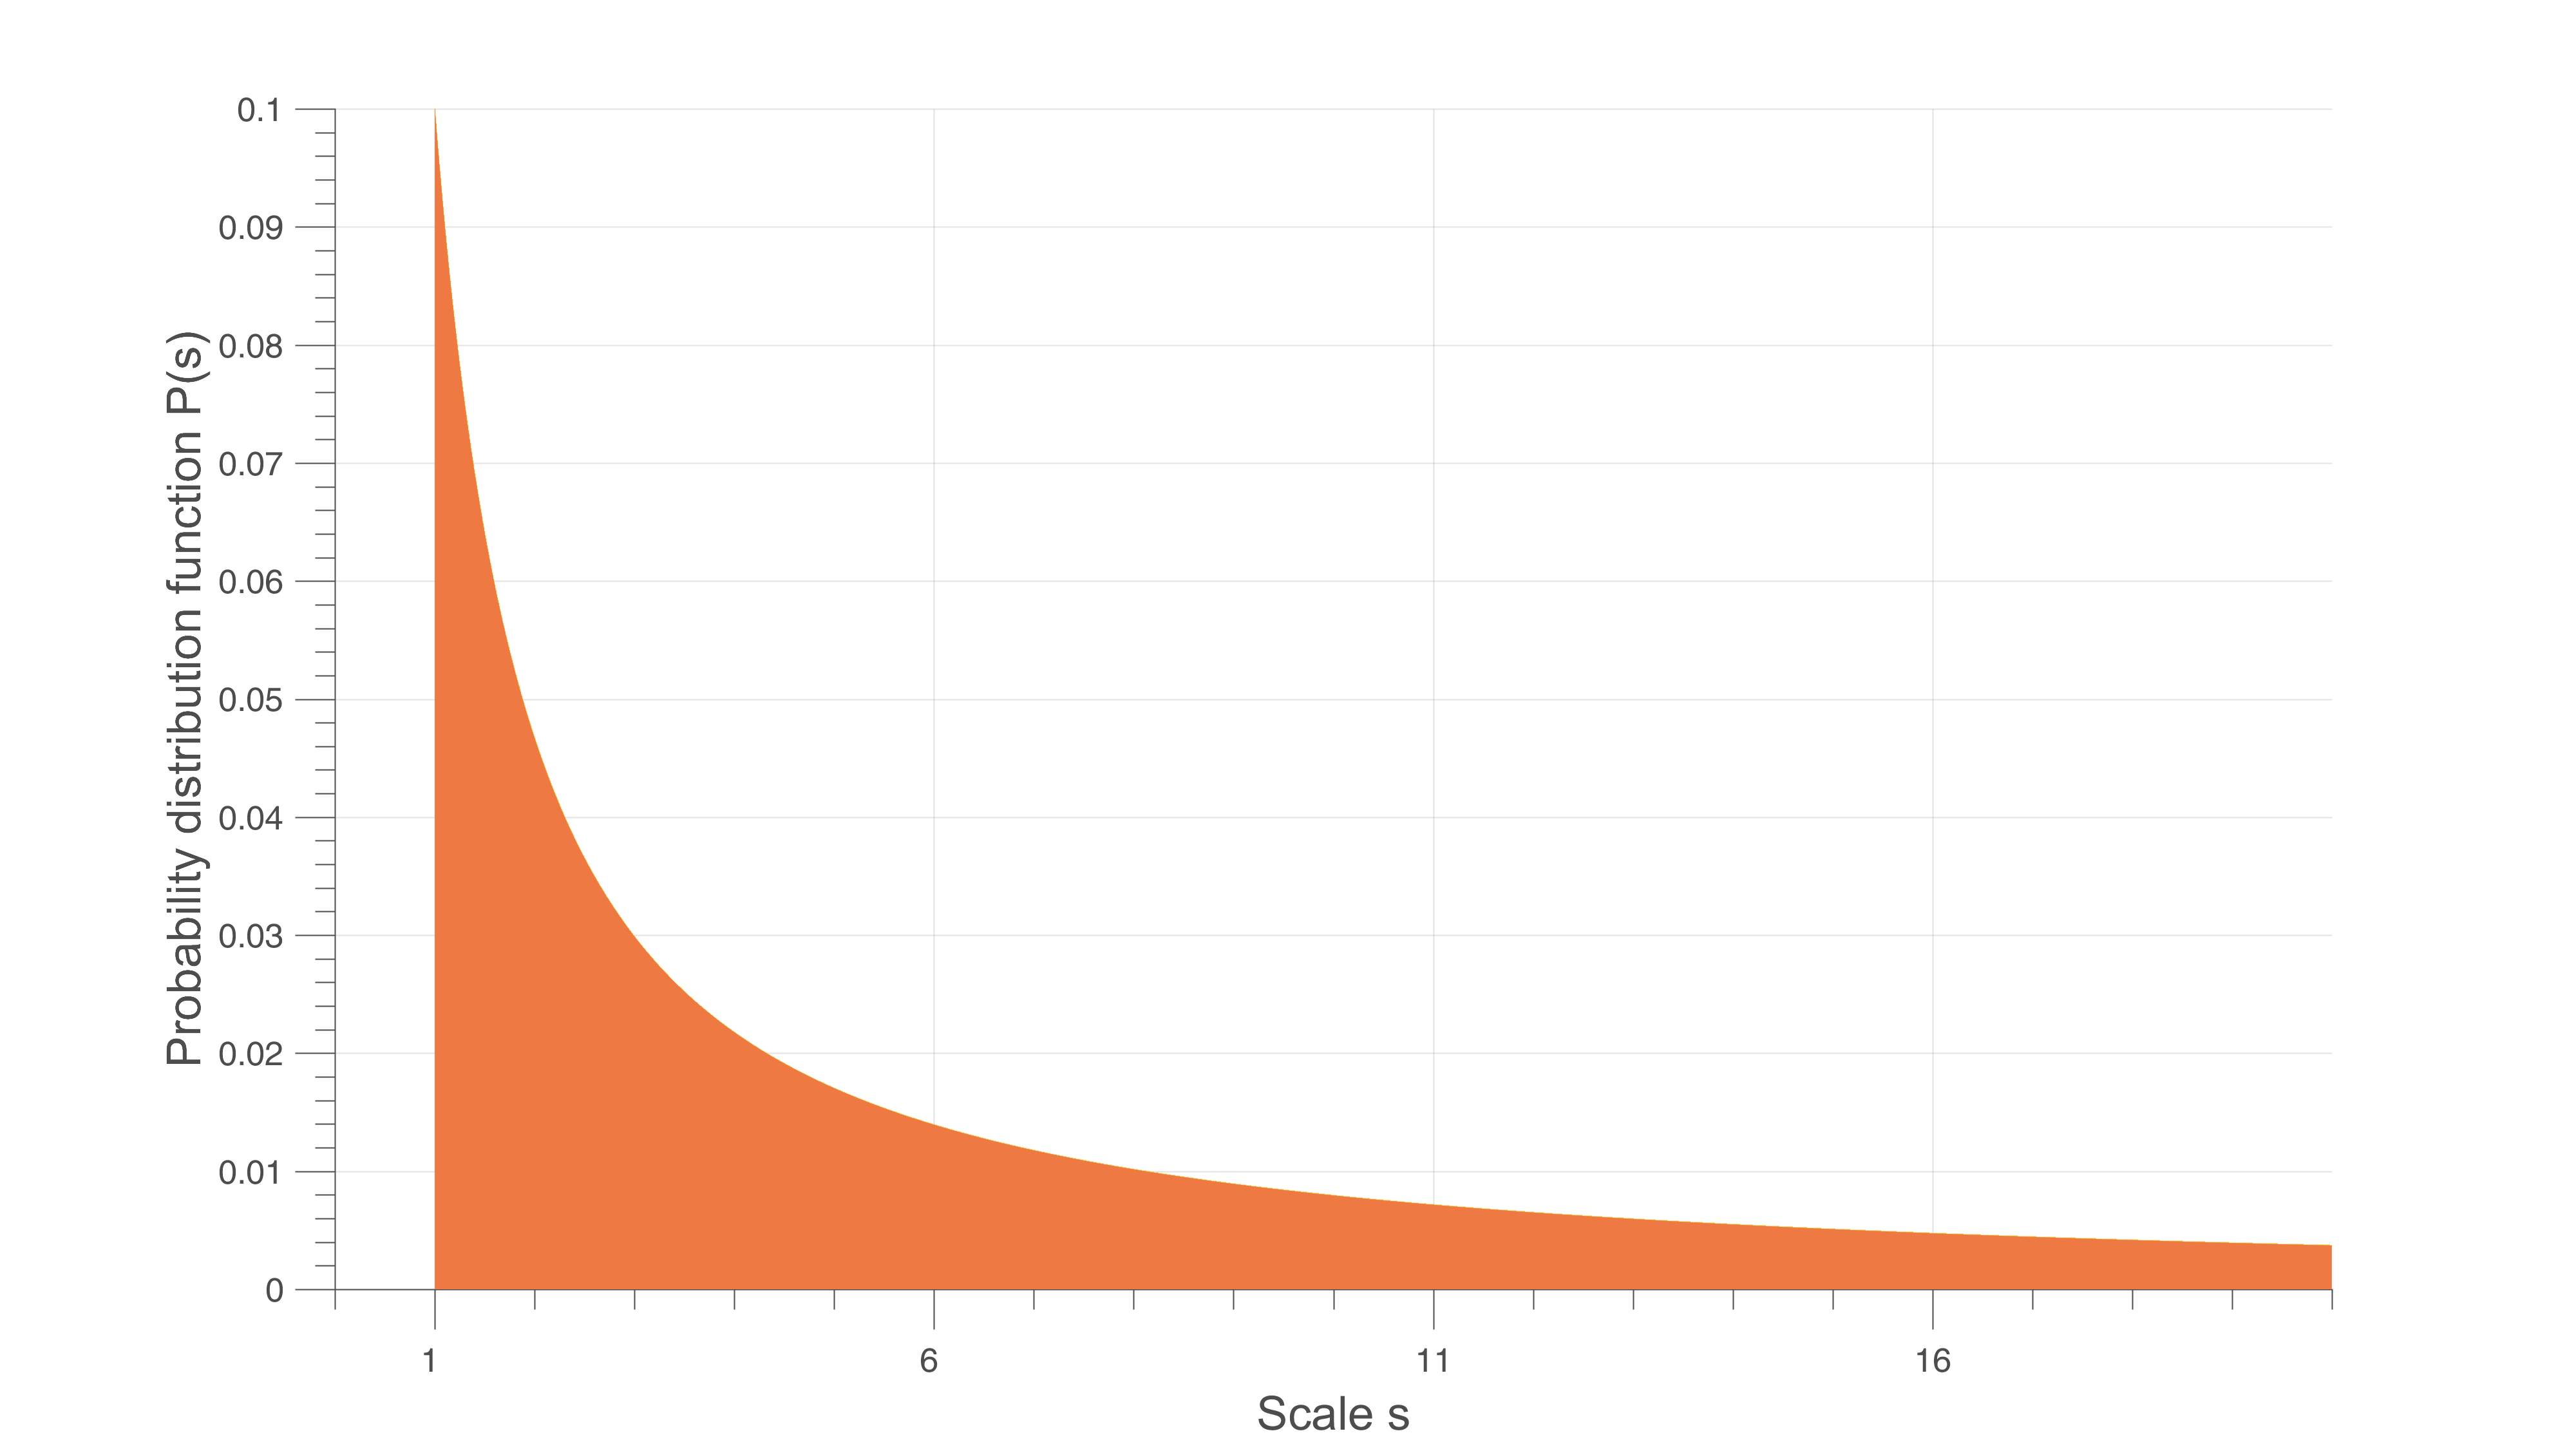
\includegraphics[width=0.9\textwidth]{figures//ps1.png} 
\caption{Weakening scales $s$ probability distribution curve when $\beta=1.5$ }
\label{ps1}
\end{figure}
\begin{figure}[!h]
\centering
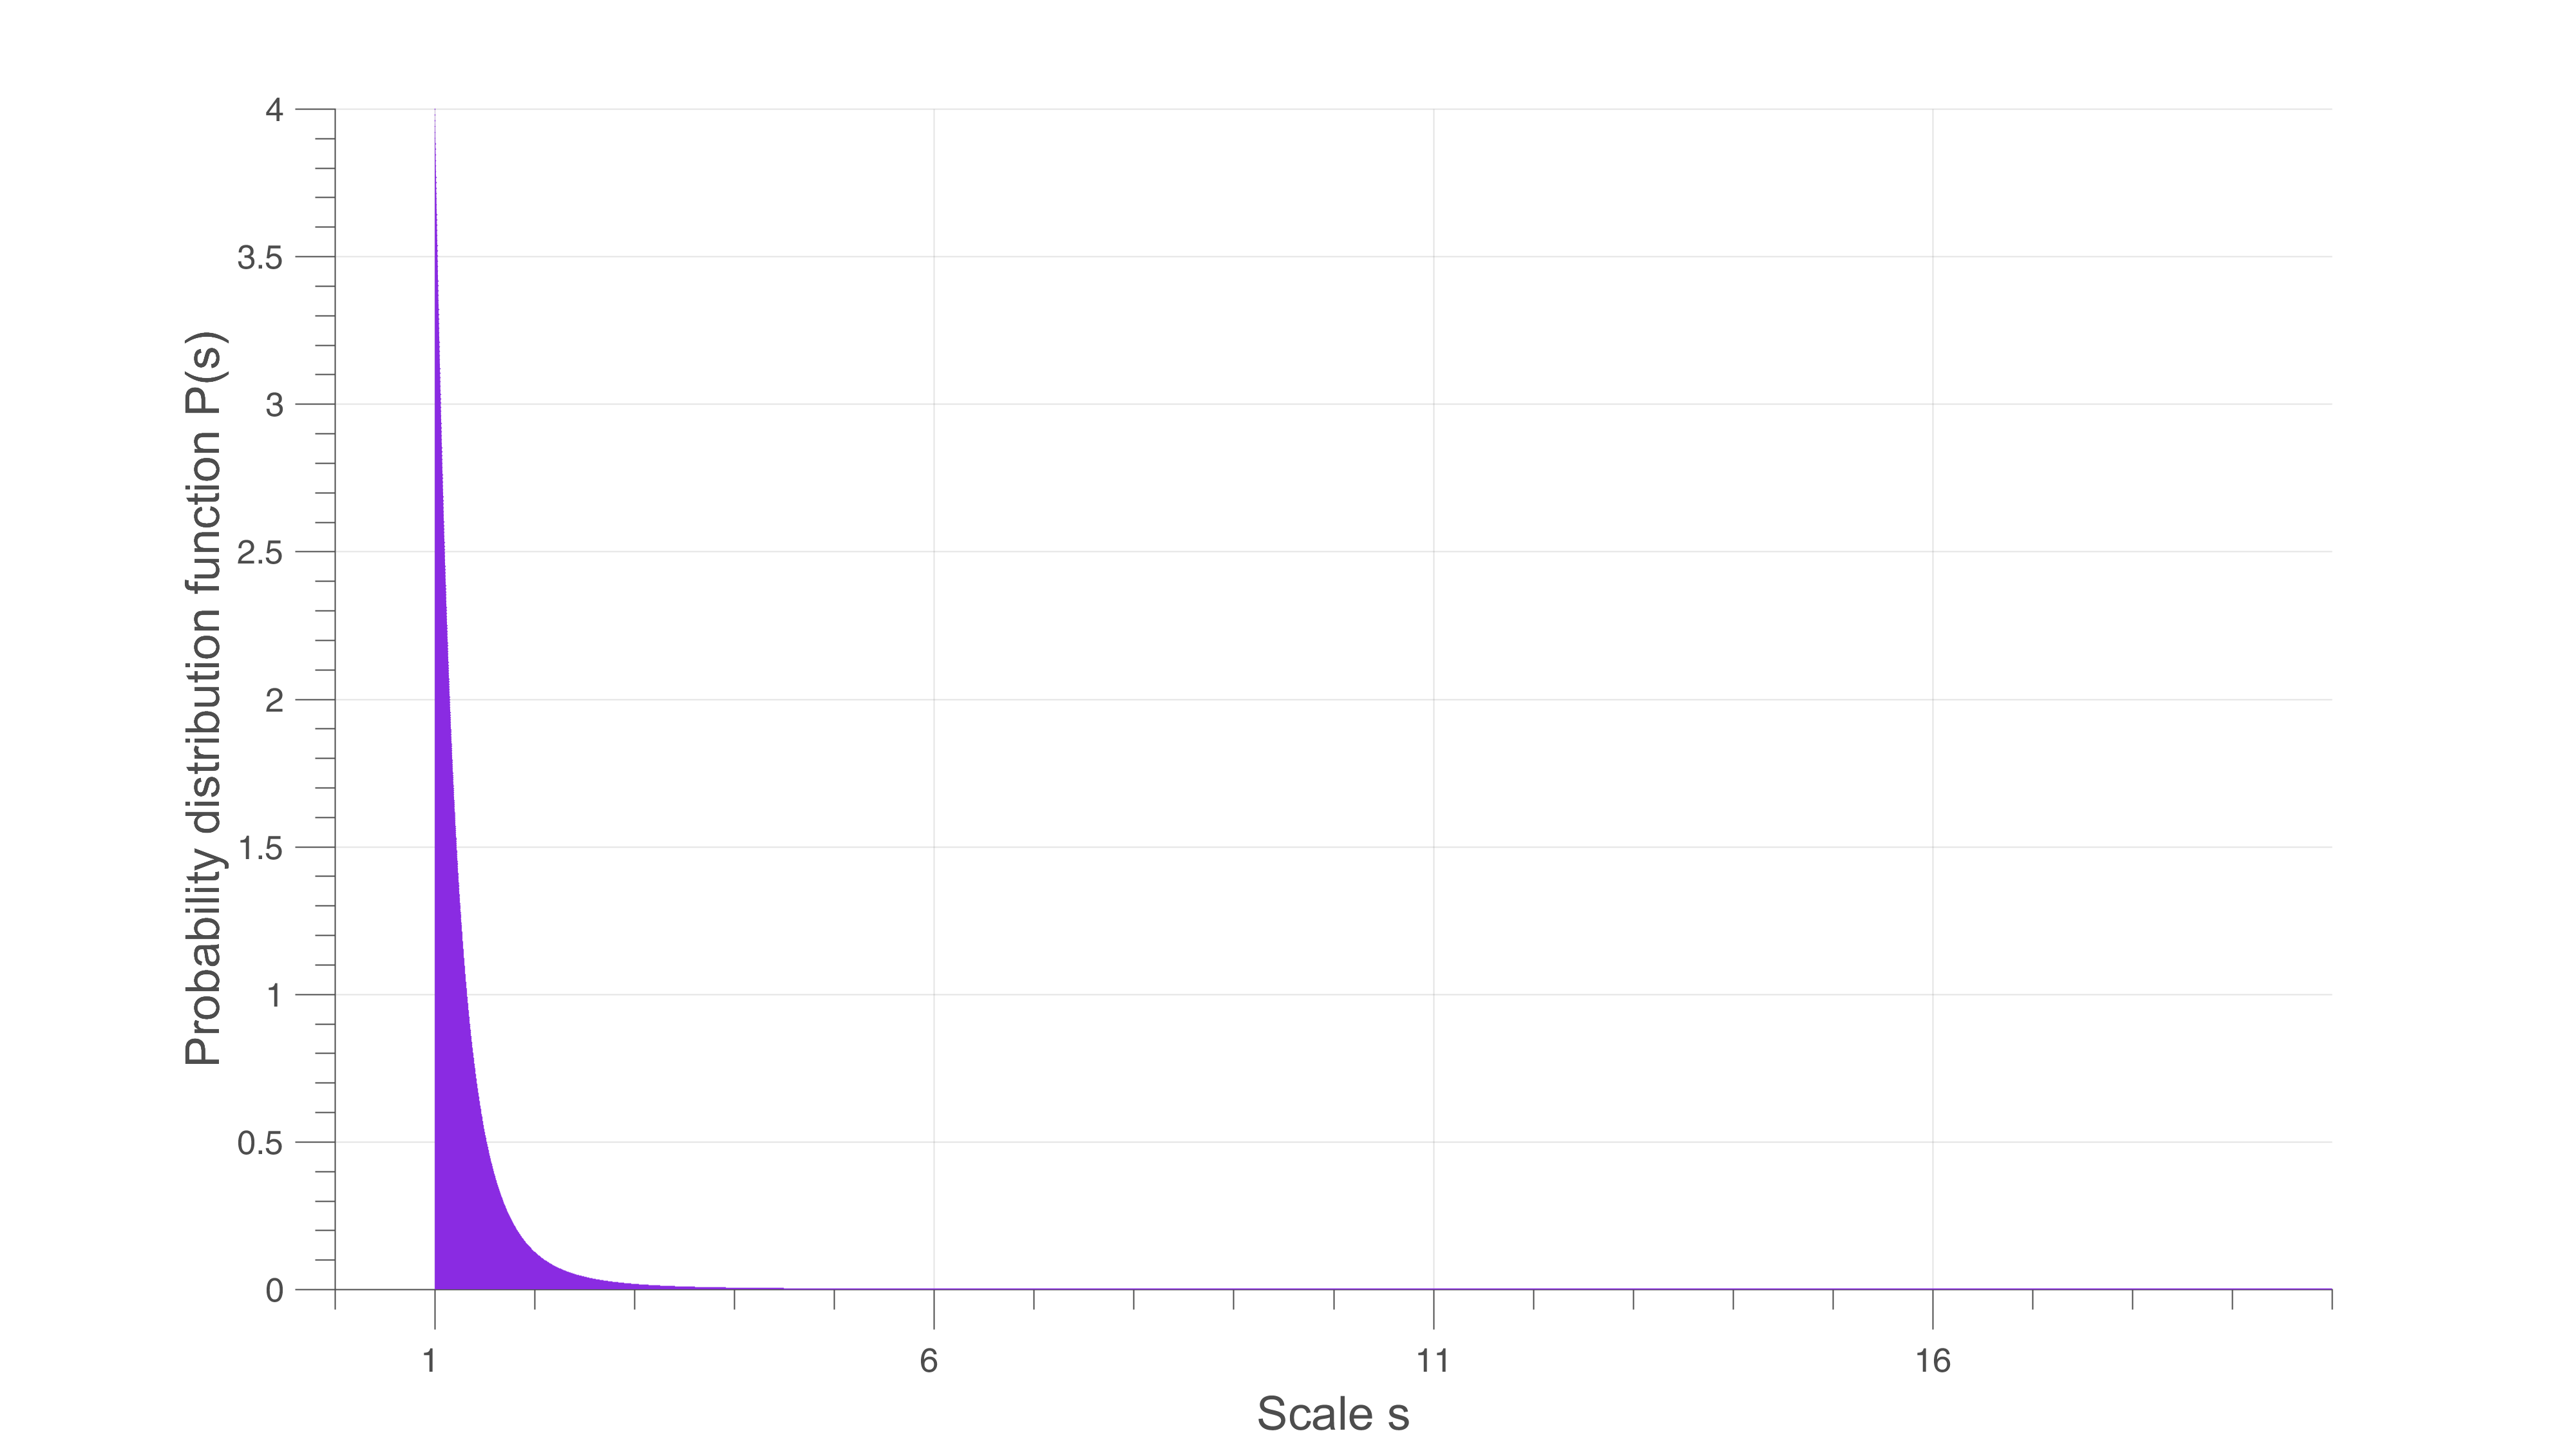
\includegraphics[width=0.9\textwidth]{figures//ps2.png} 
\caption{Weakening scales $s$ probability distribution curve when $\beta=5$ }
\label{ps2}
\end{figure}

\newpage
\subsection{Yield function with mean stress effect}
\label{sec:5.4.3}
Positive mean stress clearly reduces the fatigue life of the material. In design evaluation of multiaxial fatigue with mean stress, a simplified, conservative relation between mean stress and equivalent alternating stress is necessary. We can improve the model to come by modifying the yield function $\sigma_y$ and the localization tensor.

\vspace{6pt}
\textbf{Present choice}
\vspace{6pt}

In the model to come, our idea is to consider as in \cite{Maitournam2011232} that the yield limit $\sigma_y$ can be reduced in presence of positive mean stress. The mesoscopic yield function can therefore be written as:
\begin{equation}
f\left(s\right)=||\uline{\uline{S}}(s)-\uline{\uline{b}}(s)||+\left( \lambda \Sigma_H-\sigma_y\right) /s\leqslant 0
\label{eq.yieldfun}
\end{equation}
with $\uline{\uline{S}}$ denoting the deviatoric part of the stress tensor at microscale, and $\uline{\uline{b}}(s)$ the corresponding backstress at the same scale. The material remain in elastic regime when $f<0$ and in plastic regime when $f=0$. The parameter $\lambda$ can itself be a function of $\Sigma_H$ with a different value in traction($\lambda_+$) than in compression($\lambda_-$).


\subsection{Local plastic model}
We can now describe the mesoscopic stress state.  The model considers a plastic 
behavior at the mesoscopic scale. The mesoscopic stress evolution equations are thus:

\begin{equation}
\dot{\uline{\uline{S}}}(s,M,t)=dev\dot{\uline{\uline{\Sigma}}}(M,t)-\dfrac{E}{1+\nu}\dot{\uline{\uline{\varepsilon}}}^p(s,M,t), 
\label{eq.mesostress}
\end{equation}
which defines a Taylor-Lin scale transition model with unit localization tensor (\cite{Bosia201239}). The mesoscopic deviatoric strain rate tensor is thus equal to the macroscopic strain rate tensor $dev\dot{\uline{\uline{\Sigma}}}=\dfrac{1+\nu}{E}dev\dot{\uline{\uline{\varepsilon}}}$ with $dev\uline{\uline{\Sigma}}$ the deviatoric part of the macroscopic stress tensor. It is complemented by
\begin{equation}
\dot{\uline{\uline{b}}}(s,M,t)=\dfrac{kE}{E-k} \dot{\uline{\uline{\varepsilon}}}^p(s,M,t), 
\label{eq.backstress}
\end{equation}
which is our kinematic hardening model, and by
\begin{equation}
\dot{\uline{\uline{\varepsilon}}}^p(s,M,t)=C\dfrac{\partial f(s,M,t)}{\partial \uline{\uline{S}}}, 
\label{eq.plasticflow}
\end{equation}
which is the associated plastic flow rule assuming $C=0$ when $f<0$ and  $C\geqslant0$ when $f=0$.

Here E denotes the Young's modulus and k the hardening parameter. The local dissipated energy rate per unit volume at weakening scales $s$  is given by the local entropy dissipation:
\begin{equation}
\dot{w}(s,M,t)=(\uuline{S}-\uuline{b})(s,M,t):\uuline{\dot{\varepsilon}}^p(s,M,t).
\label{dissipated}
\end{equation}

\section{Construction of an energy based fatigue approach}
\label{sec:5.5}
In a preliminary step, we will consider a simple macroscopic loading history $\uuline{\Sigma}(M, t)$ which is uniaxial
 along direction $\uline{\uline{s}}_1$, with $\uline{\uline{s}}_1$ a given stress tensor of unit norm. In traction there is 
 $$\uline{\uline{s}}_1=\sqrt{\dfrac{3}{2}}	\left(
 \begin{array}{ccc}
2/3 & 0 & 0\\
 0 & -1/3 & 0\\ 
 0 & 0 & -1/3\\
 \end{array}\right) . $$
  Time periodic of deviatoric amplitude $S_{a}$, constant mean stress $\Sigma_{H}$ and a Von Mises flow rule are taken into account to see if we get a prediction of local failure for a number of cycles $N_F$ varying as $S_{a}^{-\gamma}.$

In uniaxial cyclic loading, there will be 3 kinds of loading patterns, as is shown in \figref{backstress}:

\vspace{6pt}
\begin{enumerate}

\item	Elastic regime, in phase 2 and 4,where we have no plastic flow $\dot{\uline{\uline{\varepsilon}}}^p(s,M,t)=\dot{\uline{\uline{b}}}=0$ ,  and where the stress is below the yield limit $|\uline{\uline{S}}-\uline{\uline{b}}|< \left( \sigma_y-\lambda \Sigma_H\right)/s$, and where we have therefore $\dot{\uline{\uline{S}}}=dev\dot{\uline{\uline{\Sigma}}}$. 
\vspace{6pt}

\item Plastic regime according to plastic flow rule, with increasing plastic deformation, in phase 5 and 1, where	$\dot{\uline{\uline{\varepsilon}}}^p(s,M,t)=\xi\dfrac{\uline{\uline{S}}(s)-\uline{\uline{b}}(s)}{||\uline{\uline{S}}(s)-\uline{\uline{b}}(s)||}> 0$ with  $\xi= \left| dev\dot{\uline{\uline{\Sigma}}}\right| \left(\dfrac{kE}{E-k}+\dfrac{E}{1+\nu} \right) ^{-1}$(detailed in annex) ,  $\uline{\uline{S}}-\uline{\uline{b}}=\uline{\uline{s}}_1 \left(\sigma_y-\lambda \Sigma_H\right)/s$ and $\dot{\uline{\uline{S}}}-\dot{\uline{\uline{b}}}=0.$ 
\vspace{6pt}

\item Plastic regime in the other direction, in phase 3, where we now have	$\dot{\uline{\uline{\varepsilon}}}^p(s,M,t)<0$,  then $\uline{\uline{S}}-\uline{\uline{b}}=-\uline{\uline{s}}_1 \left(\sigma_y-\lambda \Sigma_H\right)/s$ and $\dot{\uline{\uline{S}}}-\dot{\uline{\uline{b}}}=0$.

\end{enumerate}	

\begin{figure}[!h]
\centering
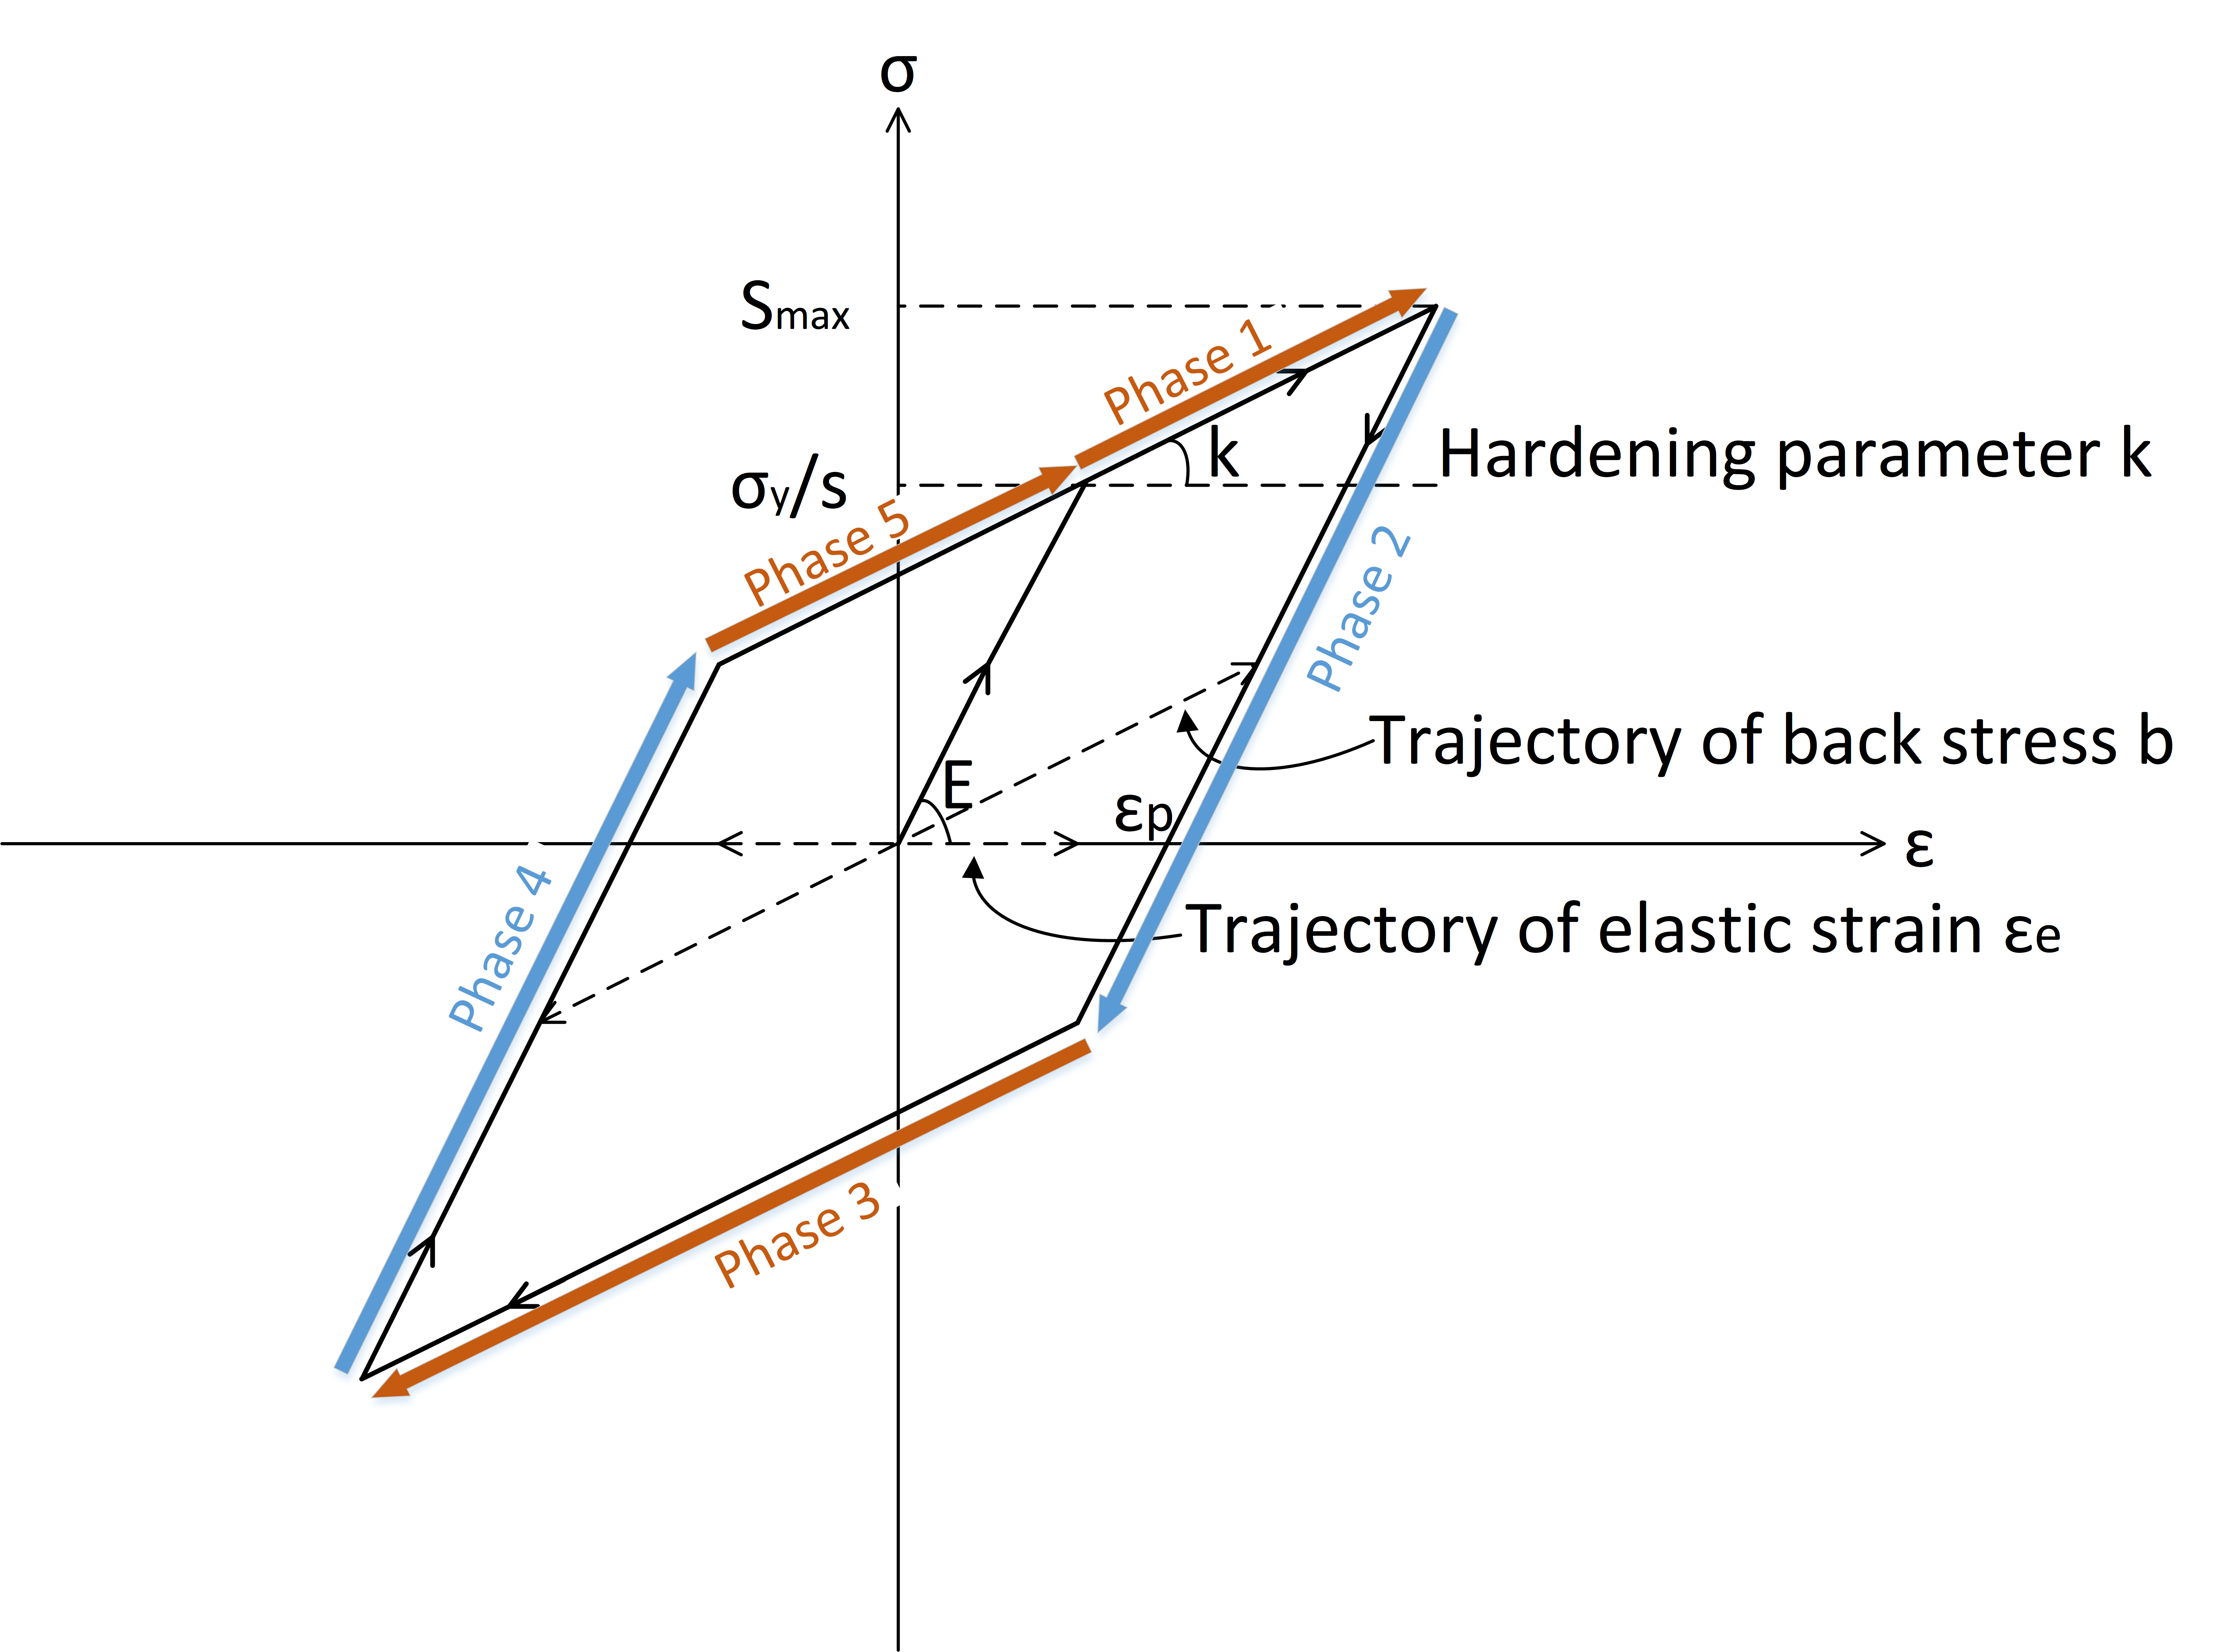
\includegraphics[width=0.9\textwidth]{figures//backstress.png} 
\caption{Uniaxial load with plastic dissipation}
\label{backstress}
\end{figure}

In phase 1, a direct analysis yields the energy dissipation at scale $s$:
\begin{equation}dW=(S-b)d\varepsilon^p=\dfrac{(E-k)(1+\nu) }{E(E+k\nu)}\dfrac{ \left(\sigma_y-\lambda \Sigma_H\right)}{s}\left(S_{a}-\dfrac{ \left(\sigma_y-\lambda \Sigma_H\right)}{s}\right).
\label{dw}
\end{equation}

A similar analysis yields $$dW(phase 1)=dW(phase 5)=\dfrac{1}{2}dW(phase 3).$$

We can then calculate  the local dissipated energy $W$  at point $M$ during one cycle by cumulating the input of all sub-scales plastic regime with their probabilities (\cite{zepeng}).
\begin{equation}
\begin{split}
W_{cyc}&=4\int_{ \left(\sigma_y-\lambda \Sigma_H\right) /S_{a}}^{\infty}dW(s,M,t)P(s)ds
\\&=4\int_{ \left(\sigma_y-\lambda \Sigma_H\right) /S_{a}}^{\infty}\dfrac{(E-k)(1+\nu) }{E(E+k\nu)}\dfrac{ \left(\sigma_y-\lambda \Sigma_H\right)}{s}\left(S_{a}-\dfrac{ \left(\sigma_y-\lambda \Sigma_H\right)}{s}\right)\left( \beta-1\right) s^{-\beta}ds
\\&=\dfrac{4(E-k)(1+\nu)\left( \beta-1\right) }{ E(E+k\nu)\beta\left( \beta+1\right) }\dfrac{S_{a}^{\beta+1}}{ \left(\sigma_y-\lambda \Sigma_H\right)^{\beta-1}}.
\end{split}
\label{eq:w}
\end{equation}

So we have a power law relationship between stress intensity and the dissipated energy per cycle.
\begin{equation}
W_{cyc}=C_1S_{a}^{\beta+1},
\label{eq.wcyc}
\end{equation}
with 
$$C_1=f(\lambda,\beta)=\dfrac{4(E-k)(1+\nu)\left( \beta-1\right) }{ E(E+k\nu)\beta\left( \beta+1\right)\left(\sigma_y-\lambda \Sigma_H\right)^{\beta-1} }.$$
If the dissipated energy accumulates until a failure value $W_0$, we can get directly the number of cycles to failure from Eq.\eqref{eq.wcyc} as:
\begin{equation}
N_{F}=\dfrac{W_0}{W_{cyc}}=\dfrac{W_0}{C_1}S_{a}^{-\beta-1}.
\label{eq.NFcyc}
\end{equation}
As for the time to failure in cyclic loading, it will be:
$$T_{F}=N_{F}t_{cyc}.$$
From Eq.\eqref{eq:w}, we then obtain that in uniaxial cyclic loading the model predicts as expected (Chapter \ref{chp:4}) a power law dependence of the number of cycles to failure in function of $S_{a}$.
However, experiments shows that the damage or the energy accumulation of a material evolves non-linearly in time and present a load dependent cycle (Chapter \ref{chp:4}). We should introduce below a method to handle such a nonlinearity.

\section{Nonlinearity of damage accumulation}
\label{sec:5.6}
\subsection{Energy approach with Chaboche law}
The Chaboche law (\cite{lemaitre1990mechanics}) is essentially a damage incremental law for cyclic loads with a deviatoric stress intensity ${A}_{\uppercase\expandafter{\romannumeral2}}$ and hydrostatic mean part $\Sigma_H$, defining the damage increase by:

\begin{equation}\delta D = \left( 1 -(1-D)^{\gamma+1}\right)^\alpha \left(\frac{{A}_{\uppercase\expandafter{\romannumeral2}} }{M(\sigma_H)\left( 1-D\right)}\right)^\gamma \delta N ,
\label{chabochemulti}
\end{equation} 

using an effective intensity ${A}_{\uppercase\expandafter{\romannumeral2}}^*={A}_{\uppercase\expandafter{\romannumeral2}}/\left( 1-D\right) $ evolving with damage $D$. And the mean stress effect is present both in exponential factor $\alpha$ and in denominator $M(\sigma_H)$.
$$\alpha=1 - a\left\langle \dfrac{\dfrac{1}{2}{A}_{\uppercase\expandafter{\romannumeral2}}-\sigma_{-1}M(\sigma_H) }{\sigma_{u} -{A}_{\uppercase\expandafter{\romannumeral2}}}\right\rangle,$$
$$M(\sigma_H) =M_0 \left(1-3c\sigma_{H,max}\right).$$

Eq.\eqref{chabochemulti} writes equivalently:
\begin{equation}\delta [1-(1-D)^{\gamma+1}]^{1-\alpha}=(1-\alpha)(\gamma+1)\left(\dfrac{{A}_{\uppercase\expandafter{\romannumeral2}} }{M(\Sigma_H)}\right)^\gamma \delta N=\dfrac{1}{N_F(\sigma)}\delta N.
\label{integration}
\end{equation}
Here $N_F(\sigma)$ denotes the number of cycles at intensity $\sigma$ to failure as obtained by integration of Eq.\eqref{integration} from $D=0$ to $D=1$. 

%
%The nonlinear damage incremental law using energy dissipation:
%\begin{equation}
%\begin{split}
%  \delta D &=\dfrac{\left( 1 -(1-D)^{\gamma+1}\right)^\alpha}{\left(1-D \right)^\gamma} \delta W
%  \\&= \dfrac{\left( 1 -(1-D)^{\gamma+1}\right)^\alpha}{\left(1-D \right)^\gamma} \dfrac{W_{cyc}\delta N}{W_0}
%  \\&= \dfrac{\left( 1 -(1-D)^{\gamma+1}\right)^\alpha}{\left(1-D \right)^\gamma} \dfrac{4(E-k)(1+\nu)\left( \beta-1\right) }{ E(E+k\nu)\beta\left( \beta+1\right) }\dfrac{S_{a}^{\beta+1}}{\left(\sigma_y-\lambda \Sigma_H\right)^{\beta-1}}\dfrac{\delta N}{W_0}.
%\end{split}
%\label{recoverchaboche}
%\end{equation} 
%
%We compare Eq.\eqref{chabochemulti} and Eq.\eqref{recoverchaboche}, in Chaboche model there is:
%$$\beta+1=\gamma. $$

Similar to Eq.\eqref{integration}, we define here the ``equivalent damage'' $\tilde{D}$(\figref{eq.Dhat}) :

\begin{equation}
\tilde{D}=1-(1-D)^{\gamma+1},
\label{eq.Dhat}
\end{equation}
with $D$ the damage variable introduced by Chaboche in its model to scale the stress intensity:
$${A}_{\uppercase\expandafter{\romannumeral2}} \longrightarrow \dfrac{{A}_{\uppercase\expandafter{\romannumeral2}}}{1-D}.$$

We have 

$\bullet$ $\tilde{D}=0$ when $D=0$ (undamaged material),

$\bullet$ $\tilde{D}=1$ when $D=1$ (failure of material),	

and a nonlinear relation in between as in \figref{fig.Dhat}:
$$\delta\tilde{D}=\left(\gamma+1 \right)\left( 1-D\right)^\gamma \delta D.$$	
\begin{figure}
\centering
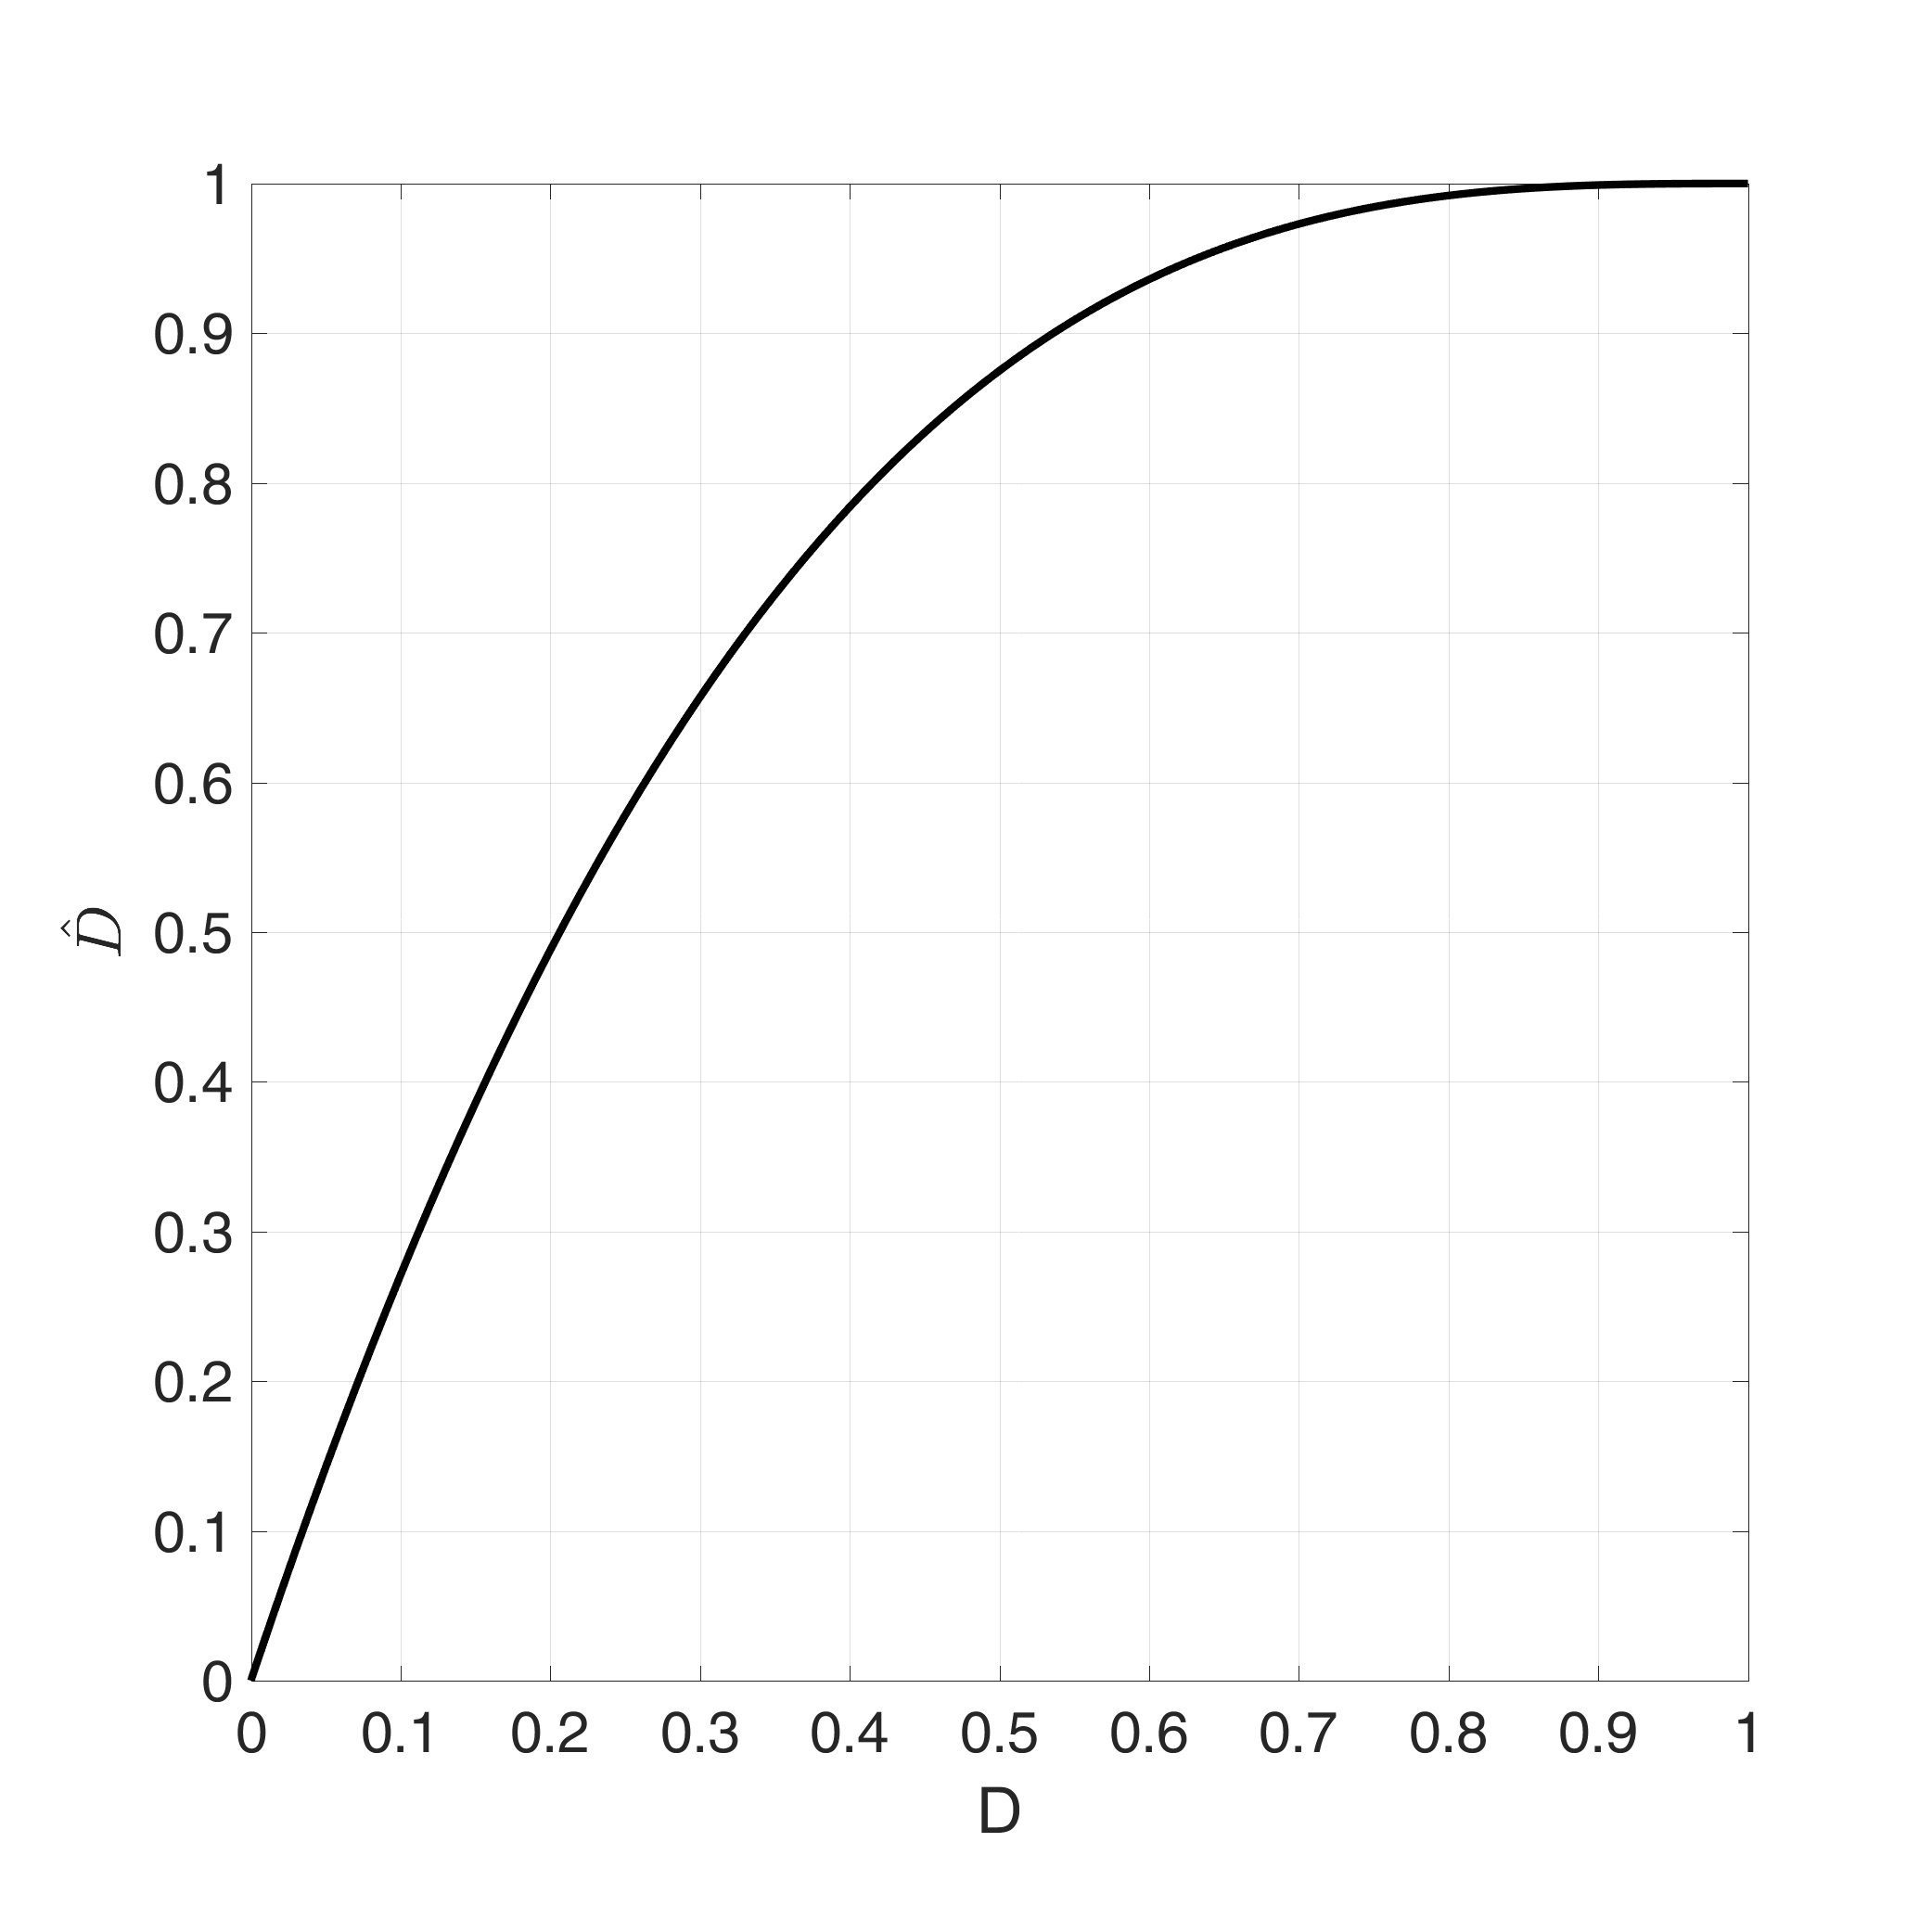
\includegraphics[width=0.6\textwidth]{figures//Dhat.png} 
\caption{The relation between $\tilde{D}$ and $D$ when $\gamma=2$}
\label{fig.Dhat}
\end{figure}

Change of damage measure $\tilde{D} = 1 - (1-D)^{\gamma+1}$ makes the evolution \eqref{chabochemulti} explicit. It writes
\begin{equation}
\dfrac{d\tilde{D}}{dN} = c_D {\tilde{D}}^\alpha \left(\dfrac{{A}_{\uppercase\expandafter{\romannumeral2}}}{M(\Sigma_{H})} \right) ^\gamma,
\label{eq.diffchaboche}
\end{equation}
yielding after integration from $\tilde{D}=0$ to $\tilde{D}=1$  a number of cycles to fatigue at constant load given by
$$
N_F =\dfrac{1}{(1-\alpha)}\left(\dfrac{{A}_{\uppercase\expandafter{\romannumeral2}}}{M(\Sigma_{H})} \right) ^{-\gamma}.
$$

This method as written requires cycle counting which is difficult and technical for complex load histories. In addition, it allows only a limited influence of multiaxiality.


Now in our model we use the same growth rule as in Chaboche in cyclic load regime, but replace stress intensity by multiscale dissipated energy  in Eq.\eqref{eq.diffchaboche}, which removes cycle counting.

The evolution \eqref{eq.diffchaboche} then writes
$$
\dfrac{d\tilde{D}}{dt} ={\tilde{D}}^\alpha \dot{W}/W_0,
$$
or in a differential form
\begin{equation}
d \tilde{D}=\tilde{D}^\alpha\dfrac{d W}{W_0}=\tilde{D}^\alpha\dfrac{W_{cyc}d N}{W_0}.
\label{eq.DWcyc}
\end{equation}

The replacement of $d W$ by $W_{cyc}dN$ is only introduced to handle cyclic loadings if they occur. The number of cycles to failure in constant loading case, obtained by integrating $\tilde{D}$ from $\tilde{D}_0$ to 1 is then:
$$N_F=\dfrac{W_0}{\left( 1-\alpha\right)W_{cyc} }\left( 1-D_0^{1-\alpha}\right) .$$
With initial damage $D_0=0$, we finally get with our proposed expression Eq.\eqref{eq.wcyc} of cyclic energy dissipation:
\begin{equation}
N_F=\dfrac{W_0}{\left( 1-\alpha\right)W_{cyc} }=\dfrac{W_0}{(1-\alpha)C_1}S_{a}^{-\beta-1}.
\label{eq.NFWcyc}
\end{equation}

From Eq.\eqref{eq.NFWcyc}, we see $(-\beta-1)=-\gamma$ is related to the slops in S-N curve and that $\dfrac{W_0}{(1-\alpha)C_1}$ defines the number of cycles to failure.
\subsection{Sequence effect}

Experiments show fatigue tests started with high stress then change to low stress has less fatigue life than the combination of high stress life proportion plus the low one. This phenomenon of sequence effect is load history dependent, so we need a stress induced parameter to describe it. 

This is done in Chaboche  with three ingredients:

\begin{enumerate} 
\vspace{6pt}
\item a damage sensitive effective stress: 
$$\sigma_D^{eff} = J_2(\uline{\uline{\Sigma}})/(1-D)={A}_{\uppercase\expandafter{\romannumeral2}}/(1-D);$$

\vspace{6pt}

\item a $(\sigma_D^{eff})^\gamma$ controlled  law for damage growth
$$\dfrac{dD}{dN} =c_\gamma {\tilde{D}}^\alpha (\sigma_D^{eff})^\gamma;$$

\vspace{6pt}

\item  a load dependence of exponent $\alpha$ (from $1$ at zero load to $0$ at large loads). In Chaboche model, the proposition of $\alpha$ is
\begin{equation}
\alpha = 1 - a\left\langle \frac{ \sigma_{eq}-\sigma_{fatigue}}{ \sigma_{u} - \sigma_{eq}}\right\rangle
\label{eq.alpchaboche}
\end{equation}
in order to recover the proper high-low sequencing effect.
\end{enumerate}

Many fatigue damage accumulation models are based on the two level loading experiments which is one of the basic random loading analysis. To facilitate the validation and interpretation of an $\alpha$ dependence on stress we will also use two-stress level loading, the specimen is firstly loaded at stress $\Sigma_1$ for $T_1$ cycles and then at stress $\Sigma_2$ for $T_2$ cycles until failure. We can then observe if the experimental results are satisfactory.

During a loading time $T_1$, we  cycle  from $\tilde{D}=0$ to $\tilde{D}= \tilde{D}_1$. By integrating Eq.\eqref{eq.DWcyc} of our proposed approach, we get:
\begin{equation}
\left( 1-\tilde{D}_1\right) ^{1-\alpha_1}=\dfrac{T_1}{T_{F1}},
\label{23a}
\end{equation}
with $T_{F1}$ the time to failure with this loading.

Then we cycle from  ${\tilde D}={\tilde D}_1$ to failure ${\tilde D}=1$, which yields
\begin{equation}
1-\left( 1-\tilde{D}_1\right)^{1-\alpha_2}=\dfrac{T_2}{T_{F2}}.
\label{23b}
\end{equation}

From Eq.\eqref{23a} and Eq.\eqref{23b}, after elimination of $\left( 1-D_1\right)$ we get:
\begin{equation} 
\dfrac{T_2}{T_{F2}} =1-\left( \dfrac{T_1}{T_{F1}}\right) ^\eta,
\label{eq.sequence}
\end{equation}
with
\begin{equation}
\eta=\dfrac{1-\alpha_2}{1-\alpha_1}.
\label{eq.eta}
\end{equation}

In the case of high-low loading sequence we have $\Sigma_1>\Sigma_2$,  which gives $\alpha_1<\alpha_2$, so it comes to:
$$\eta=\frac{1-\alpha_2}{1-\alpha_1}<1 \implies
\frac{T_2}{T_{F2}}=1-\left( \frac{T_1}{T_{F1}}\right) ^\eta<1-\frac{T_1}{T_{F1}} \implies
\frac{T_1}{T_{F1}}+\frac{T_2}{T_{F2}}<1.$$

The $\alpha$ dependence on stress intensity does therefore predict a sequencing effect where a low loading sequence following a high one will reduce the life of the structure if $\alpha$ decreases when the load increases.

To get the same effect in our construction, we propose here to introduce $s_{min}$, which is the minimum scale that experiences plastic dissipation thus causes energy loss:
\begin{equation}
s_{min}=\dfrac{\left(\sigma_y-\lambda \Sigma_H\right)}{S_{a}}.
\label{eq.smin}
\end{equation}

We propose a load dependent $\alpha$ through $s_{min}$. Possible choice
of $\alpha$ is expressed as Eq.\eqref{eq.alpha}:
\begin{equation}
\alpha=1-a\left( \dfrac{\frac{1}{s_{min}}}{1-\frac{1}{s_{min}}} \right) .
\label{eq.alpha}
\end{equation}

There is no notion of fatigue limit in our model, $\sigma_{faigue}=0$. The intensity of loading
$$\frac{ \sigma_{eq}-\sigma_{fatigue}}{ \sigma_{u} - \sigma_{eq}}= \frac{ 1}{\frac{\sigma_{u}}{\sigma_{eq}} -1}$$
is measured by 
$$\left( \dfrac{\frac{1}{s_{min}}}{1-\frac{1}{s_{min}}}\right) =\left(s_{min}-1 \right) ^{-1}.$$
This means that we measure the distance of load to ultimate failure by local variable $s_{min}$ through 

$$\frac{\sigma_{u}}{\sigma_{eq}} -1 \longrightarrow \left( s_{min}-1\right)  $$


We can see from \figref{fig.sequence} that with our proposition, cycling $1$ for fifty percent of its failure time leaves a reserve before failure to cycling $2$ of much less than fifty percent. To conclude, the cumulative damage under high-low loading sequence, as we deduced, has the addition of partial lives less than unit. Similarly, the cumulative damage under low-high loading sequence has addition of partial lives more than 1:
$$\frac{T_1}{T_{F1}}+\frac{T_2}{T_{F2}}>1.$$
The curve in both cases is depicted in \figref{fig.sequence}.
\begin{figure}[!h]
\centering
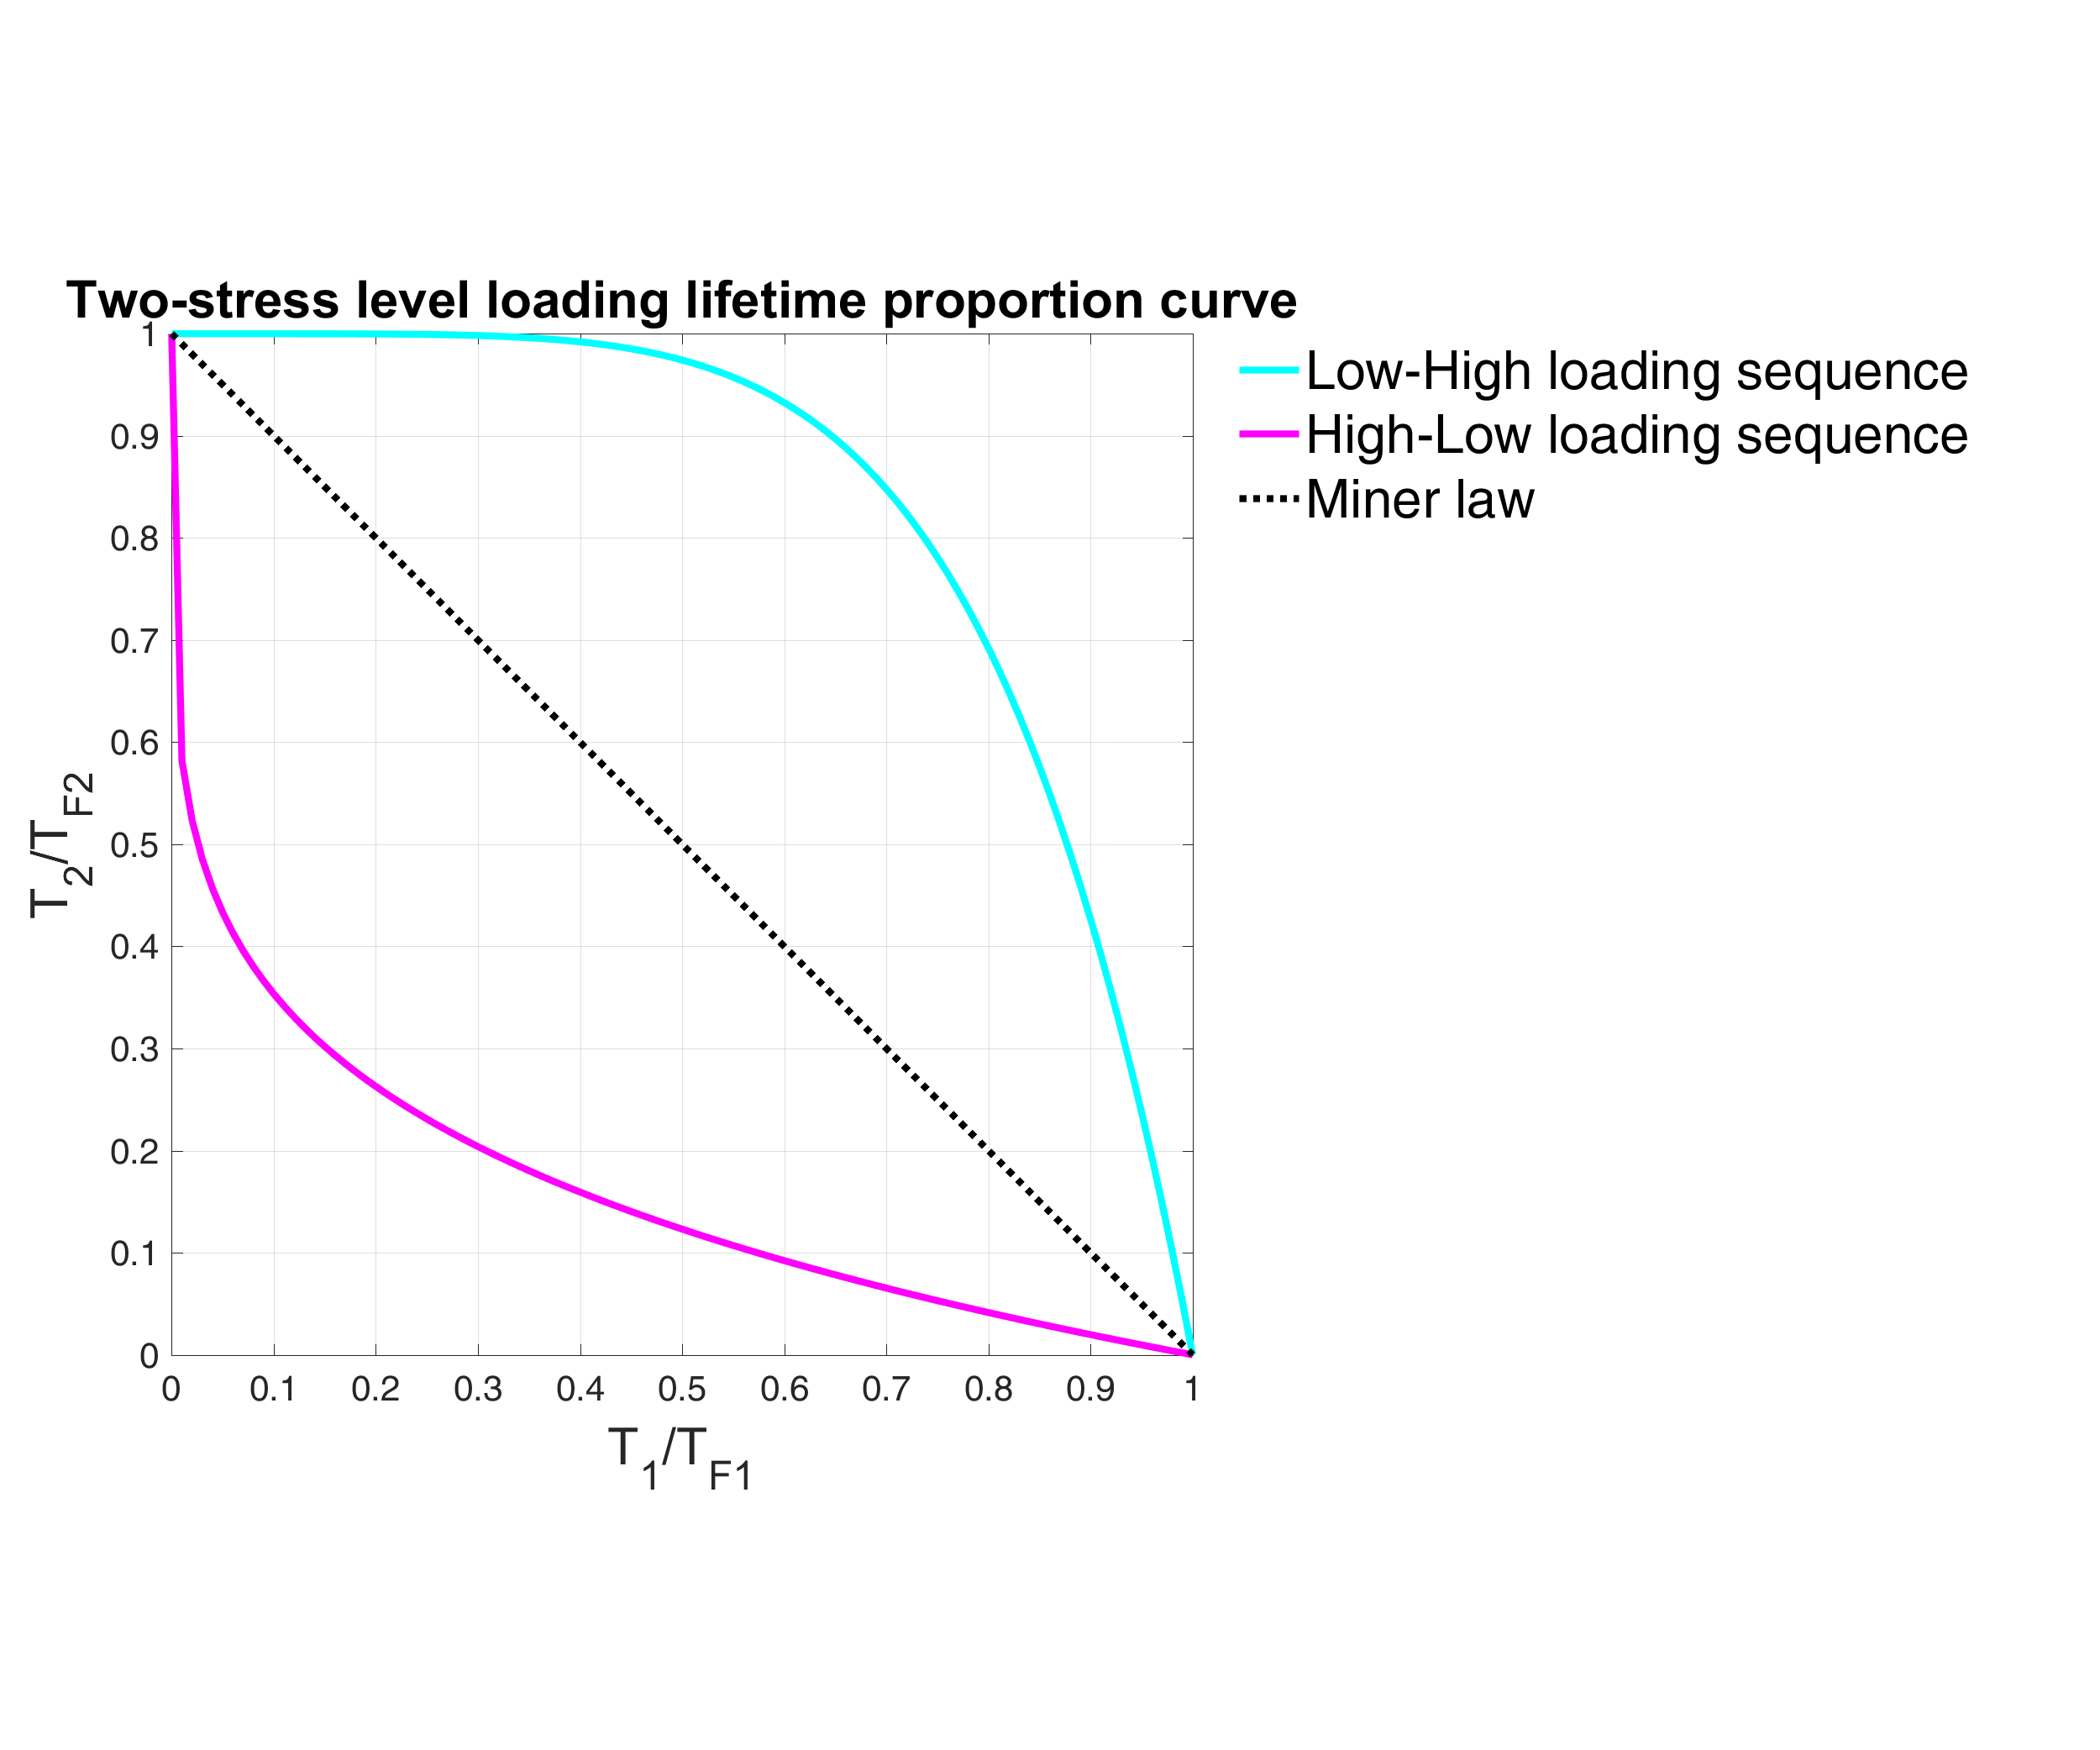
\includegraphics[width=0.8\textwidth]{figures//sequence.png} 
\caption{High to low and low to high loading sequence comparison in 4-point bending($F_{low}=5000 N, F_{high}=30000 N, Radius=0.2m, \Sigma_u=1.67E8$), with the proposed damage accumulation law (Eq.\eqref{eq.DWcyc}) induced equation Eq.\eqref{eq.sequence} and Chaboche type $\alpha$ (Eq.\eqref{eq.alpchaboche}) containing Crossland criterion}
\label{fig.sequence}
\end{figure}
For constant two-level stress loading, $\alpha_1=\alpha_2$, the Chaboche law returns to the Miner rule when $F_{low}=F_{high}$ where:
$$\frac{T_1}{T_{F1}}+\frac{T_2}{T_{F2}}=1.$$

\newpage
\subsection{The final model}
\label{sec:5.6.3}
In summary, our damage based fatigue life criterion using a damage evolution governed by a multiscale plastic energy dissipation, has four ingredients.
\begin{itemize}
\item  a scale dependent yield limit $$\frac{1}{s} (\sigma_y- \lambda \Sigma_H^{macro})$$ associated to a microscopic plastic evolution governed by the standard plastic evolution laws Eq.\eqref{eq.mesostress} - Eq.\eqref{eq.plasticflow};

\vspace{6pt}	

\item a multiscale plastic energy dissipation obtained by summing plastic dissipation across our power law scale distribution
\begin{equation}
\dot{W}(M,t)=\int_{s=1}^{\infty}\left(\uline{\uline{S}}-\uline{\uline{b}} \right) (s,M,t):\uline{\uline{\dot{\varepsilon}}}^p(s,M,t) s^{-\beta}ds;
\label{eq.final2}
\end{equation}

\vspace{6pt}	

\item a load intensity sequencing effect that we have represented by the formula : 
\begin{equation}
1 - \alpha = a (s_{min}-1)^{-f};
\label{eq.final3}
\end{equation}

\vspace{6pt}	

\item a exponential damage evolution law with load dependent exponent $\alpha$ given by the above formula and coefficient $\dot{W}/W_0$ governed by the multiscale plastic dissipation rate: 
\begin{equation}
\dfrac{d\tilde{D}}{dt} ={\tilde{D}}^\alpha \dot{W}/W_0.
\label{eq.final4}
\end{equation}
\end{itemize}

In this model we have five independent coefficients in addition to the construction of the local plastic model Eq.\eqref{eq.mesostress} - Eq.\eqref{eq.plasticflow} :

\begin{enumerate}
\item reference density of damage energy : $W_0$ (in MPa)

\item mean stress effect coefficient : $\lambda$
\item slope of SN curve : $\beta+1$

\item sensitivity to load intensity $a$. 
\item exponent in the load sequence effect $f$. 
\end{enumerate}

\newpage
\section{Numerical strategy}
\label{sec:5.7}
\subsection{Scale discretization}
We now need to propose a practical implementation strategy for our final model of section \ref{sec:5.6.3}.Our first approach takes one cycle as unit time. We compute analytically by Eq.\eqref{eq:w} the energy dissipation at each scale during this cycle. The method is valid for simple loading history and which includes the integration on all weakening scales. The damage $\tilde{D}$ is then accumulated after each cycle by numerical integration of Eq.\eqref{eq.final4} until we get to the fatigue limit of $\tilde{D}=1$.

However, there are certain limitations of this method. Firstly we need a load history decomposition in cycles. Secondly in real life the perfect close loop cycle is hardly applicable. Finally, we need to approximate $\alpha$  by its average value per cycle which is computed numerically and can not be done analytically.

Thus we propose in a more general method which can be integrated by a step by step strategy. We compute numerically the dissipation at different scales using an implicit Euler time integration of the constitutive laws of section \ref{sec:5.4.4}. After which we make a numerical integration on different scales. Then we can update the damage and go to next time step. 

Instead of doing the scale integration directly which can be difficult for complex loading, the Gaussian Quadrature rule with Legendre points is used to give the value of local dissipated energy rate. To use the Gaussian quadrature rule the limit range of integral must be from $-1$ to $1$, while the total dissipated energy  is expressed by integrating all the weakening scale $s$ ranging from 1 to infinity with their occurrence probabilities:
$$\dot{W}=\int_{1}^{\infty}\dot{w}(s) (\beta-1)(s)^{-\beta}ds.$$

\noindent
To change the limit range of integral from $[1,\infty]$ to $[1,0]$ we take as new integration variable
$u(s)= s^{1-\beta}$. Therefore the dissipated energy summed on all scales is:
\begin{equation}
\begin{split}
\dot{W}&=\int_{1}^{\infty}\dot{w}(s) (\beta-1)(s)^{-\beta}ds
\\&=\int_{0}^{1}\dot{w}\left( u^{\frac{1}{1-\beta}}\right)du
\\&=\frac{1}{2}\int_{-1}^{1}\dot{w}\left[  \left( \frac{x+1}{2}\right) ^{\frac{1}{1-\beta}}\right] dx
\end{split}
\label{allscale}
\end{equation}
given $u=\dfrac{x+1}{2}$. So the dissipated energy rate integrated over all scales takes the form of Eq.\eqref{allscalerate}:
\begin{equation}
\dot{W}=\frac{1}{2}\int_{-1}^{1}\dot{w}\left[  \left( \frac{x+1}{2}\right) ^{\frac{1}{1-\beta}},t\right] dx\approx\frac{1}{2}\sum_{i}\omega_i\dot{w}\left[  \left( \frac{x_i+1}{2}\right) ^{\frac{1}{1-\beta}},t\right],
\label{allscalerate}
\end{equation}
where $\omega_i$ and $x_i$ are respectively the weights and nodes of the Gauss Legendre integration rule used for the numerical integration.  In this work, we used a 64 points Gaussian Legendre integration rule (\cite{Legendre}) with $s_i=\left( \dfrac{x_i+1}{2}\right) ^{\frac{1}{1-\beta}}$ being the associated scale.

\subsection{Calculation of local plastic dissipation}
\label{sec:5.4.4}
The material could be both in elastic and plastic regime depending on the considered scale. To be more elaborate, we reuse the fundamental equations in different regimes. At scale $s$, we have a dissipation rate given by:
$$\dot{w}(s)=\left( \uline{\uline{S}}-\uline{\uline{b}}\right):\dot{\uline{\uline{\varepsilon}}}^p, $$
which differs between plastic and elastic regime.

\vspace{6pt}
\noindent
\textbf{Elastic regime:}

\vspace{6pt}
\noindent
There we have
plastic strain rate
$\dot{\uline{\uline{\varepsilon}}}^p=0$, back stress rate $\dot{\uline{\uline{b}}}=0$ and deviatoric stress rate $\dot{\uline{\uline{S}}}=dev\dot{\uline{\uline{\Sigma}}}$, leading to
$$\dot{\uline{\uline{S}}}-\dot{\uline{\uline{b}}}=dev\dot{\uline{\uline{\Sigma}}},$$ 
meaning
$$\left( \uline{\uline{S}}-\uline{\uline{b}}\right) (t+dt)=\left( \uline{\uline{S}}-\uline{\uline{b}}\right) (t)+dev\dot{\uline{\uline{\Sigma}}}dt.$$
At each time step we define a trial stress:
\begin{equation}
\left( \uline{\uline{S}}-\uline{\uline{b}}\right)_{trial}:=\left( \uline{\uline{S}}-\uline{\uline{b}}\right)(t+dt).
\label{trial}
\end{equation}
We are in elastic regime at scale $s$ as long as we satisfy

\begin{equation}
\left| \left|  \uline{\uline{S}}-\uline{\uline{b}}\right| \right| _{trial}\leqslant\left( \sigma_y-\lambda \Sigma_H\right)/s.
\label{eq.trialelastic}
\end{equation}

\vspace{6pt}
\noindent
\textbf{Plastic regime:}
\vspace{6pt}

\noindent
When we leave elastic regime at scale s, i.e. when the above inequality Eq.\eqref{eq.trialelastic} is violated, we have:
\begin{numcases}{}
\dot{\uline{\uline{\varepsilon}}}^p=\xi\dfrac{\uline{\uline{S}}-\uline{\uline{b}}}{\left| \left|\uline{\uline{S}}-\uline{\uline{b}}\right| \right|}, \xi>0, & plastic   flow, \label{plasticflow}
\\
\left| \left|\uline{\uline{S}}-\uline{\uline{b}}\right| \right|= \left(\sigma_y-\lambda \Sigma_H\right)/s, & yield   limit,\label{yieldlimit}
\\
\left( \uline{\uline{S}}-\uline{\uline{b}}\right) :\left( \dot{\uline{\uline{S}}}-\dot{\uline{\uline{b}}}\right) =0, & yield   limit   time invariance,
\\
\dot{\uline{\uline{b}}}=\dfrac{kE}{E-k}\dot{\uline{\uline{\varepsilon}}}^p, & kinematic   hardening  rule, \label{kinematichardening}
\\
\dot{\uline{\uline{S}}}=dev\dot{\uline{\uline{\Sigma}}}-\dfrac{E}{1+\nu} \dot{\uline{\uline{\varepsilon}}}^p, & localisation  rule. \label{localisation}
\end{numcases}

In all cases, we get by integrating Eq.\ref{localisation}, Eq.\ref{kinematichardening} with the use of Eq.\ref{plasticflow}.
\begin{equation}
\left( \uline{\uline{S}}-\uline{\uline{b}}\right) (s,t+dt)=\dfrac{\left( \uline{\uline{S}}-\uline{\uline{b}}\right)_{trial} (s,t+dt)}{1+\eta},
\end{equation}

and because of the yield condition Eq.\ref{yieldlimit}, we have
 $$\eta=max\left\lbrace \underbrace{0}_{elastic\; regime}, \underbrace{\dfrac{\left| \left|\uline{\uline{S}}-\uline{\uline{b}}\right| \right|_{trial}}{ \left(\sigma_y-\lambda \Sigma_H\right)/s}-1}_{plastic \; regime\; when\; this\; number\; is\; positive}\right\rbrace, $$

That is to say, when the structure is in elastic regime at time $t$ and scale $s$, we have $\left( \uline{\uline{S}}-\uline{\uline{b}}\right)(s,t)=\left( \uline{\uline{S}}-\uline{\uline{b}}\right)_{trial} (s,t)$. Otherwise, if  the norm of $\left( \uline{\uline{S}}-\uline{\uline{b}}\right)_{trial} (s,t)$ is greater than the local yield limit $ \left(\sigma_y-\lambda \Sigma_H\right)/s$, $\left( \uline{\uline{S}}-\uline{\uline{b}}\right)(s,t)$ will be projected on the yield limit. 

Knowing the distinction between elastic and plastic regime under multiple scales, we compute the general expression of the dissipated energy rate at scale $s$.
\begin{equation}
\dot{w}(s)=\left( \uline{\uline{S}}-\uline{\uline{b}}\right) :\dot{\uline{\uline{\varepsilon}}}^p=\gamma\dfrac{  \left(\sigma_y-\lambda \Sigma_H\right)}{s}.
\label{w}
\end{equation}

From Eq.\eqref{eta} and Eq.\eqref{eta2} in annex, we get:

\begin{equation}
	\begin{split}
		E\gamma dt&=\left\langle \left| \left|\uline{\uline{S}}-\uline{\uline{b}}\right| \right|_{trial}-\dfrac{ \left(\sigma_y-\lambda \Sigma_H\right)}{s}\right\rangle /\left(\dfrac{1}{1+\nu}+\dfrac{k}{E-k} \right)
		\\&=\left\langle \left| \left|\uline{\uline{S}}-\uline{\uline{b}}\right| \right|_{trial}-\dfrac{ \left(\sigma_y-\lambda \Sigma_H\right)}{s}\right\rangle\dfrac{(E-k)(1+\nu) }{(E+k\nu)},
	\end{split}
	\label{gamma}
\end{equation}
where $\langle$ $\rangle$ is Macaulay bracket symbol defined as $\langle m\rangle=0$ if $m\leqslant0$, otherwise $\langle m\rangle=m$. Thus the dissipated energy rate only depends on the evolution of the variable $\left( \uline{\uline{S}}-\uline{\uline{b}}\right)$, which must therefore be mentioned during the whole cycle under study.

We replace $\gamma$ deduced from Eq.\eqref{gamma} in Eq.\eqref{w} to give the expression of local energy dissipation rate at scale $s$:
\begin{equation}
\dot{w}(s)dt=\dfrac{(E-k)(1+\nu) }{E(E+k\nu)}\left\langle  \left| \left|\uline{\uline{S}}-\uline{\uline{b}}\right| \right|_{trial}-\dfrac{ \left(\sigma_y-\lambda \Sigma_H\right)}{s}\right\rangle \dfrac{ \left(\sigma_y-\lambda \Sigma_H\right)}{s}.
\label{dW}
\end{equation}

With Eq.\eqref{allscalerate}, the final expression of energy dissipation $W$ during time step $dt$ writes:

\begin{equation}
\begin{split}
W&=\dot{W}dt
\\&=\frac{1}{2}\sum_{i}\omega_i\dot{w}\left[  \left( \frac{x+1}{2}\right) ^{\frac{1}{1-\beta}}\right]dt
\\&=\dfrac{(E-k)(1+\nu) }{2E(E+k\nu)}\sum_{i}\omega_i\left\langle  \left| \left|\uline{\uline{S}}-\uline{\uline{b}}\right| \right|_{trial}-\dfrac{\left(\sigma_y-\lambda \Sigma_H\right) }{\left( \dfrac{x_i+1}{2}\right) ^{\frac{1}{1-\beta}}}\right\rangle \dfrac{\left(\sigma_y-\lambda \Sigma_H\right) }{\left( \dfrac{x_i+1}{2}\right)^{\frac{1}{1-\beta}}}.
\end{split}
\label{finaldw}
\end{equation}

The mean stress effect term in Chaboche model is $s_{-1}\left(1-3\dfrac{\sigma_H}{\sigma_u} \right)$, where the fatigue limit at zero mean stress $s_{-1}$ is reduced in the presence of $\sigma_H$. In our model, the yield limit decreases with positive mean stress. Because of the presence of the term $\lambda \Sigma_H$ which will be positive when $\Sigma_H$ is positive. In Eq.\ref{finaldw}, the coefficient $\lambda$ can change values if $\Sigma_H$ changes sign (see section \ref{sec:5.4.3}).


\subsection{Damage integration algorithm}

Numerically the  change of $\alpha$ is extremely nonlinear with time. From \figref{fig.alpmean} we can see the mean value of $\alpha$ depends on loading pattern. 

\begin{figure}[!h]
	\centering
	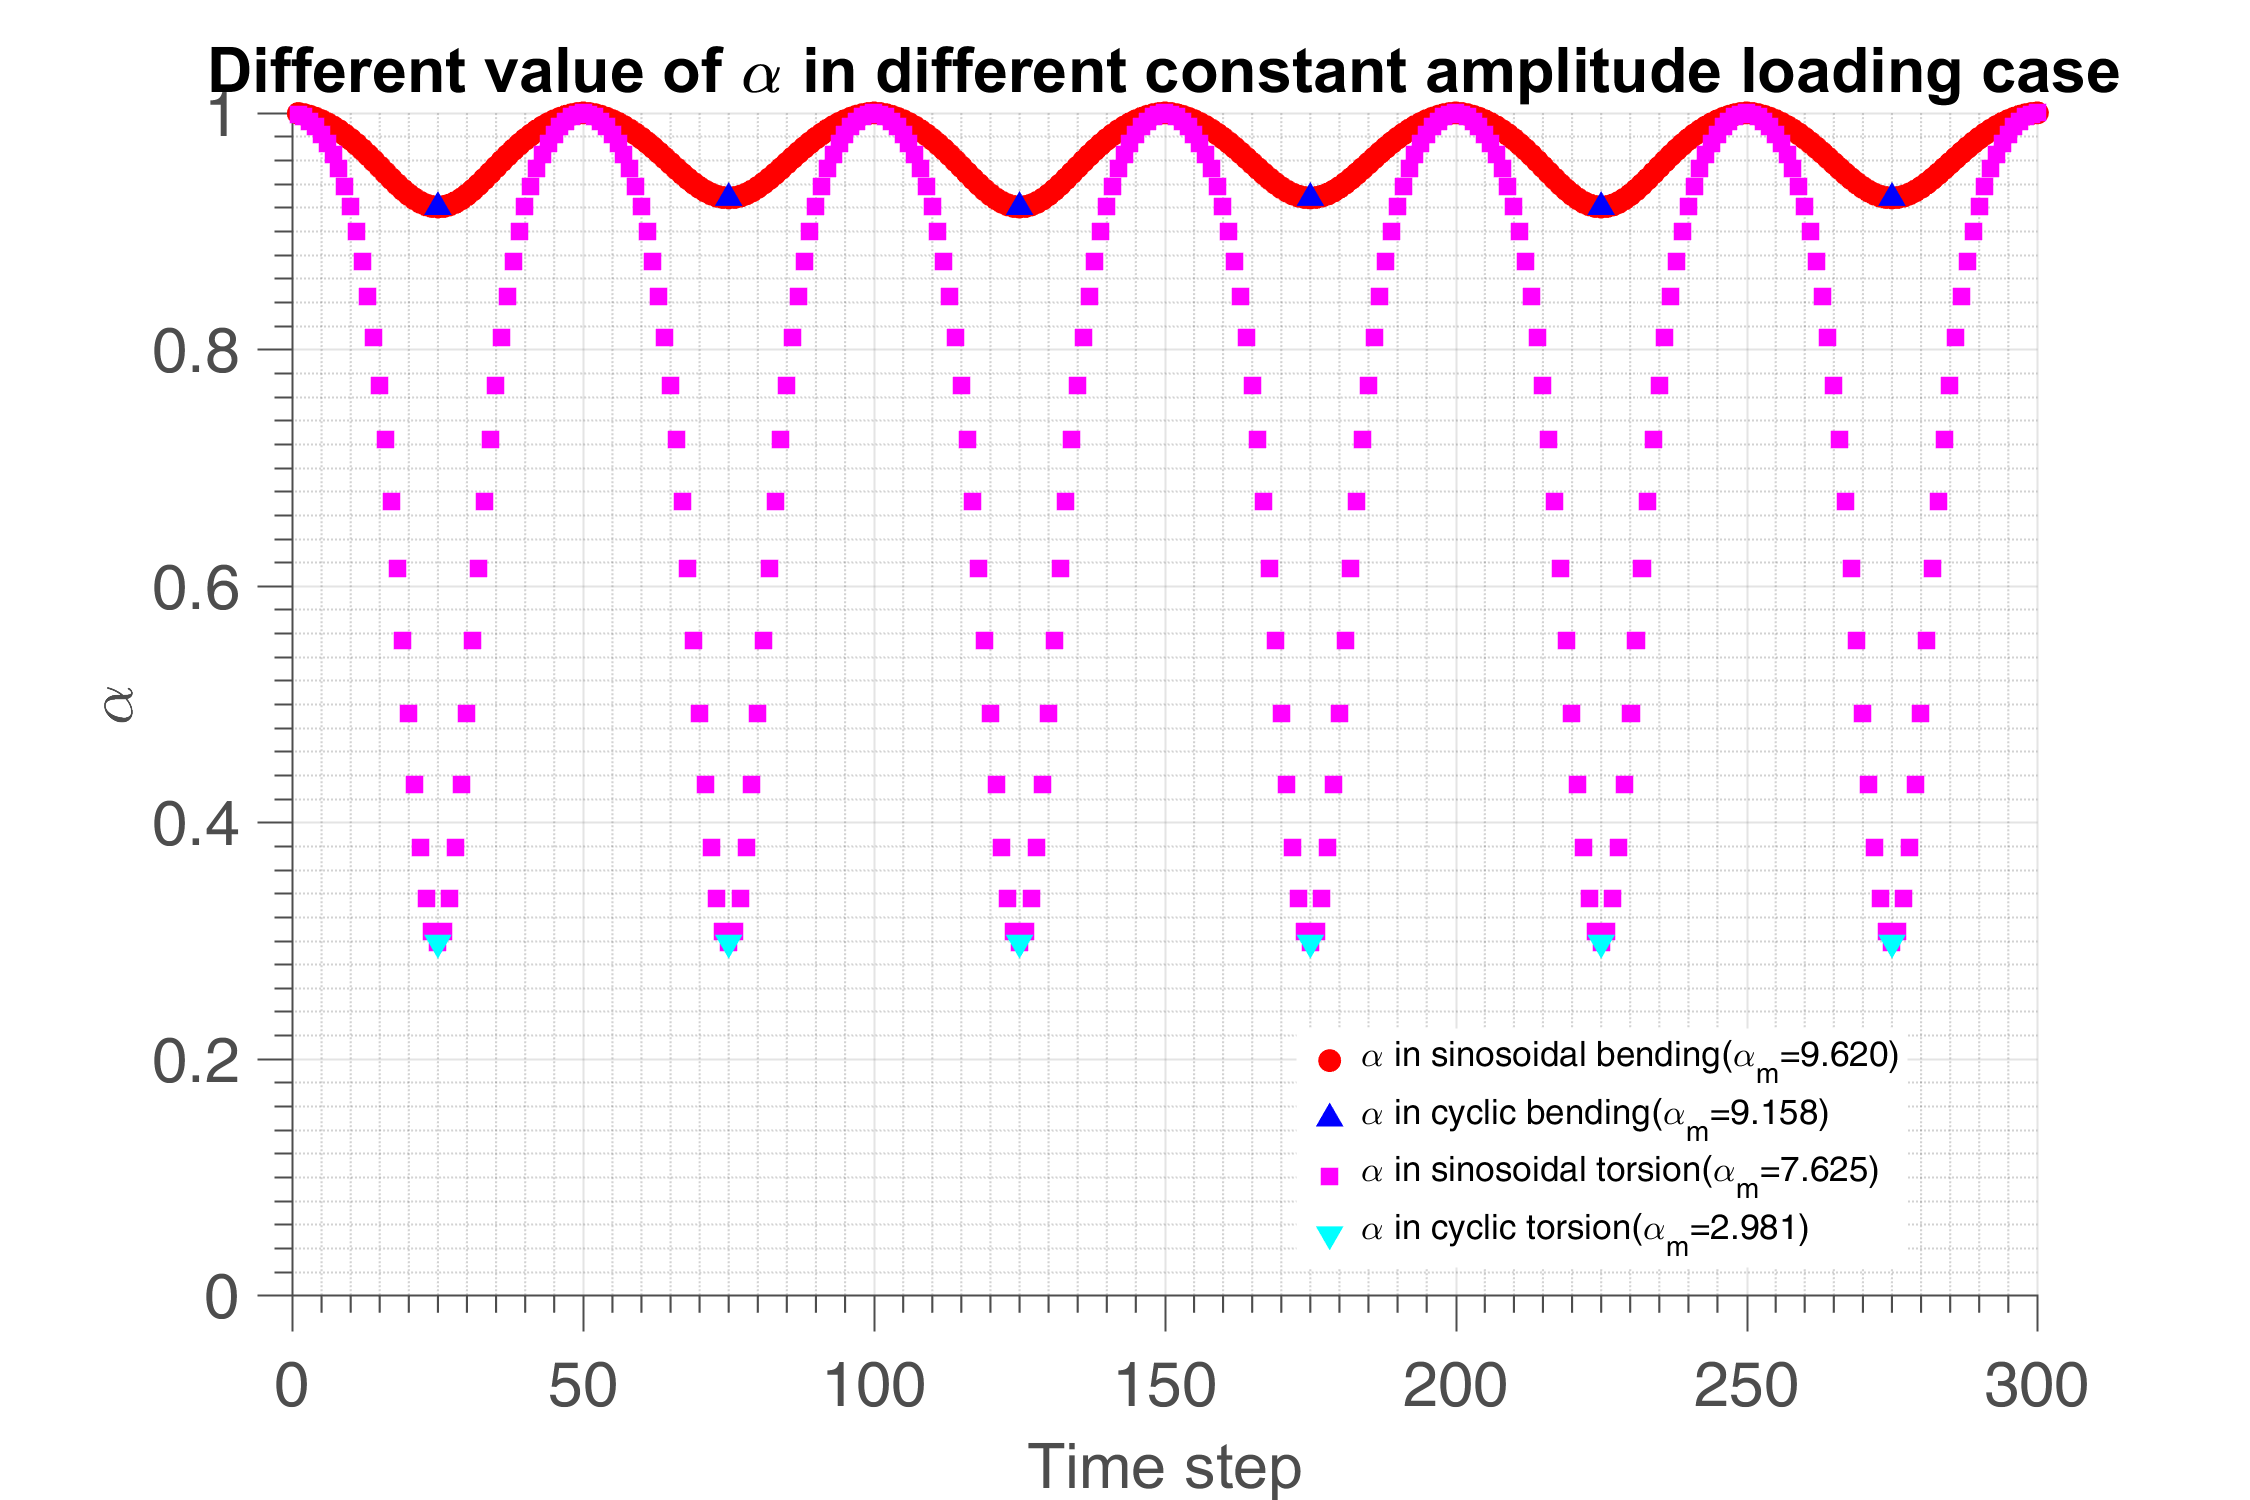
\includegraphics[width=0.8\textwidth]{figures//alp_mean_methods.png} 
	\caption{The evolution of $\alpha$ in bending and torsion with $\Sigma_y=1080 MPa$, $\Sigma_{bending}=\Sigma_{torsion}=500 MPa$, $a=0.3$ and $200$ time steps in one cycle}
	\label{fig.alpmean}
\end{figure}


Because of the possible large variations in time  of $\alpha$, the evolution problem in damage is very nonlinear and thus, one needs to develop and validate an improved numerical time integration strategy at least  for two specific cases: the constant amplitude case and the random load case.

We propose in constant amplitude load with very small evolution of damage per cycle to numerically calculate $W_{cyc}$ and the mean values of $\alpha$ through one cycle or several cycles(out-of-phase condition) and apply the result to life prediction by using  Eq.\eqref{eq.NFWcyc}:
\begin{equation}
N_F= \dfrac{W_0}{\left( 1-\alpha_m\right) W_{cyc}},
\label{eq.cycNF}
\end{equation}
which is obtained by direct integration of our damage law assuming time uniform dissipation in one cycle and frozen $\alpha$.
In this way the numerical cost is not as high as for the numerical implementation of all the loading points in random loading case. Because of the symmetrical shape of the evolution of $\alpha$, numerically the mean value of $\alpha$ does not strongly depend on the number of steps per cycle. In the verification process we have compared $100\sim1000$ time steps per cycle (\figref{fig.sn-num-ana}). 

For complex cyclic load cases, the idea is to accurately compute the history of plastic dissipation during one cycle (multiscale calculation with time refinement), and to use this precomputed result in the time integration of the scalar damage evolution law with a time stepping which is adapted to the time variation of $\alpha$. 

\begin{figure}[!h]
	\centering
	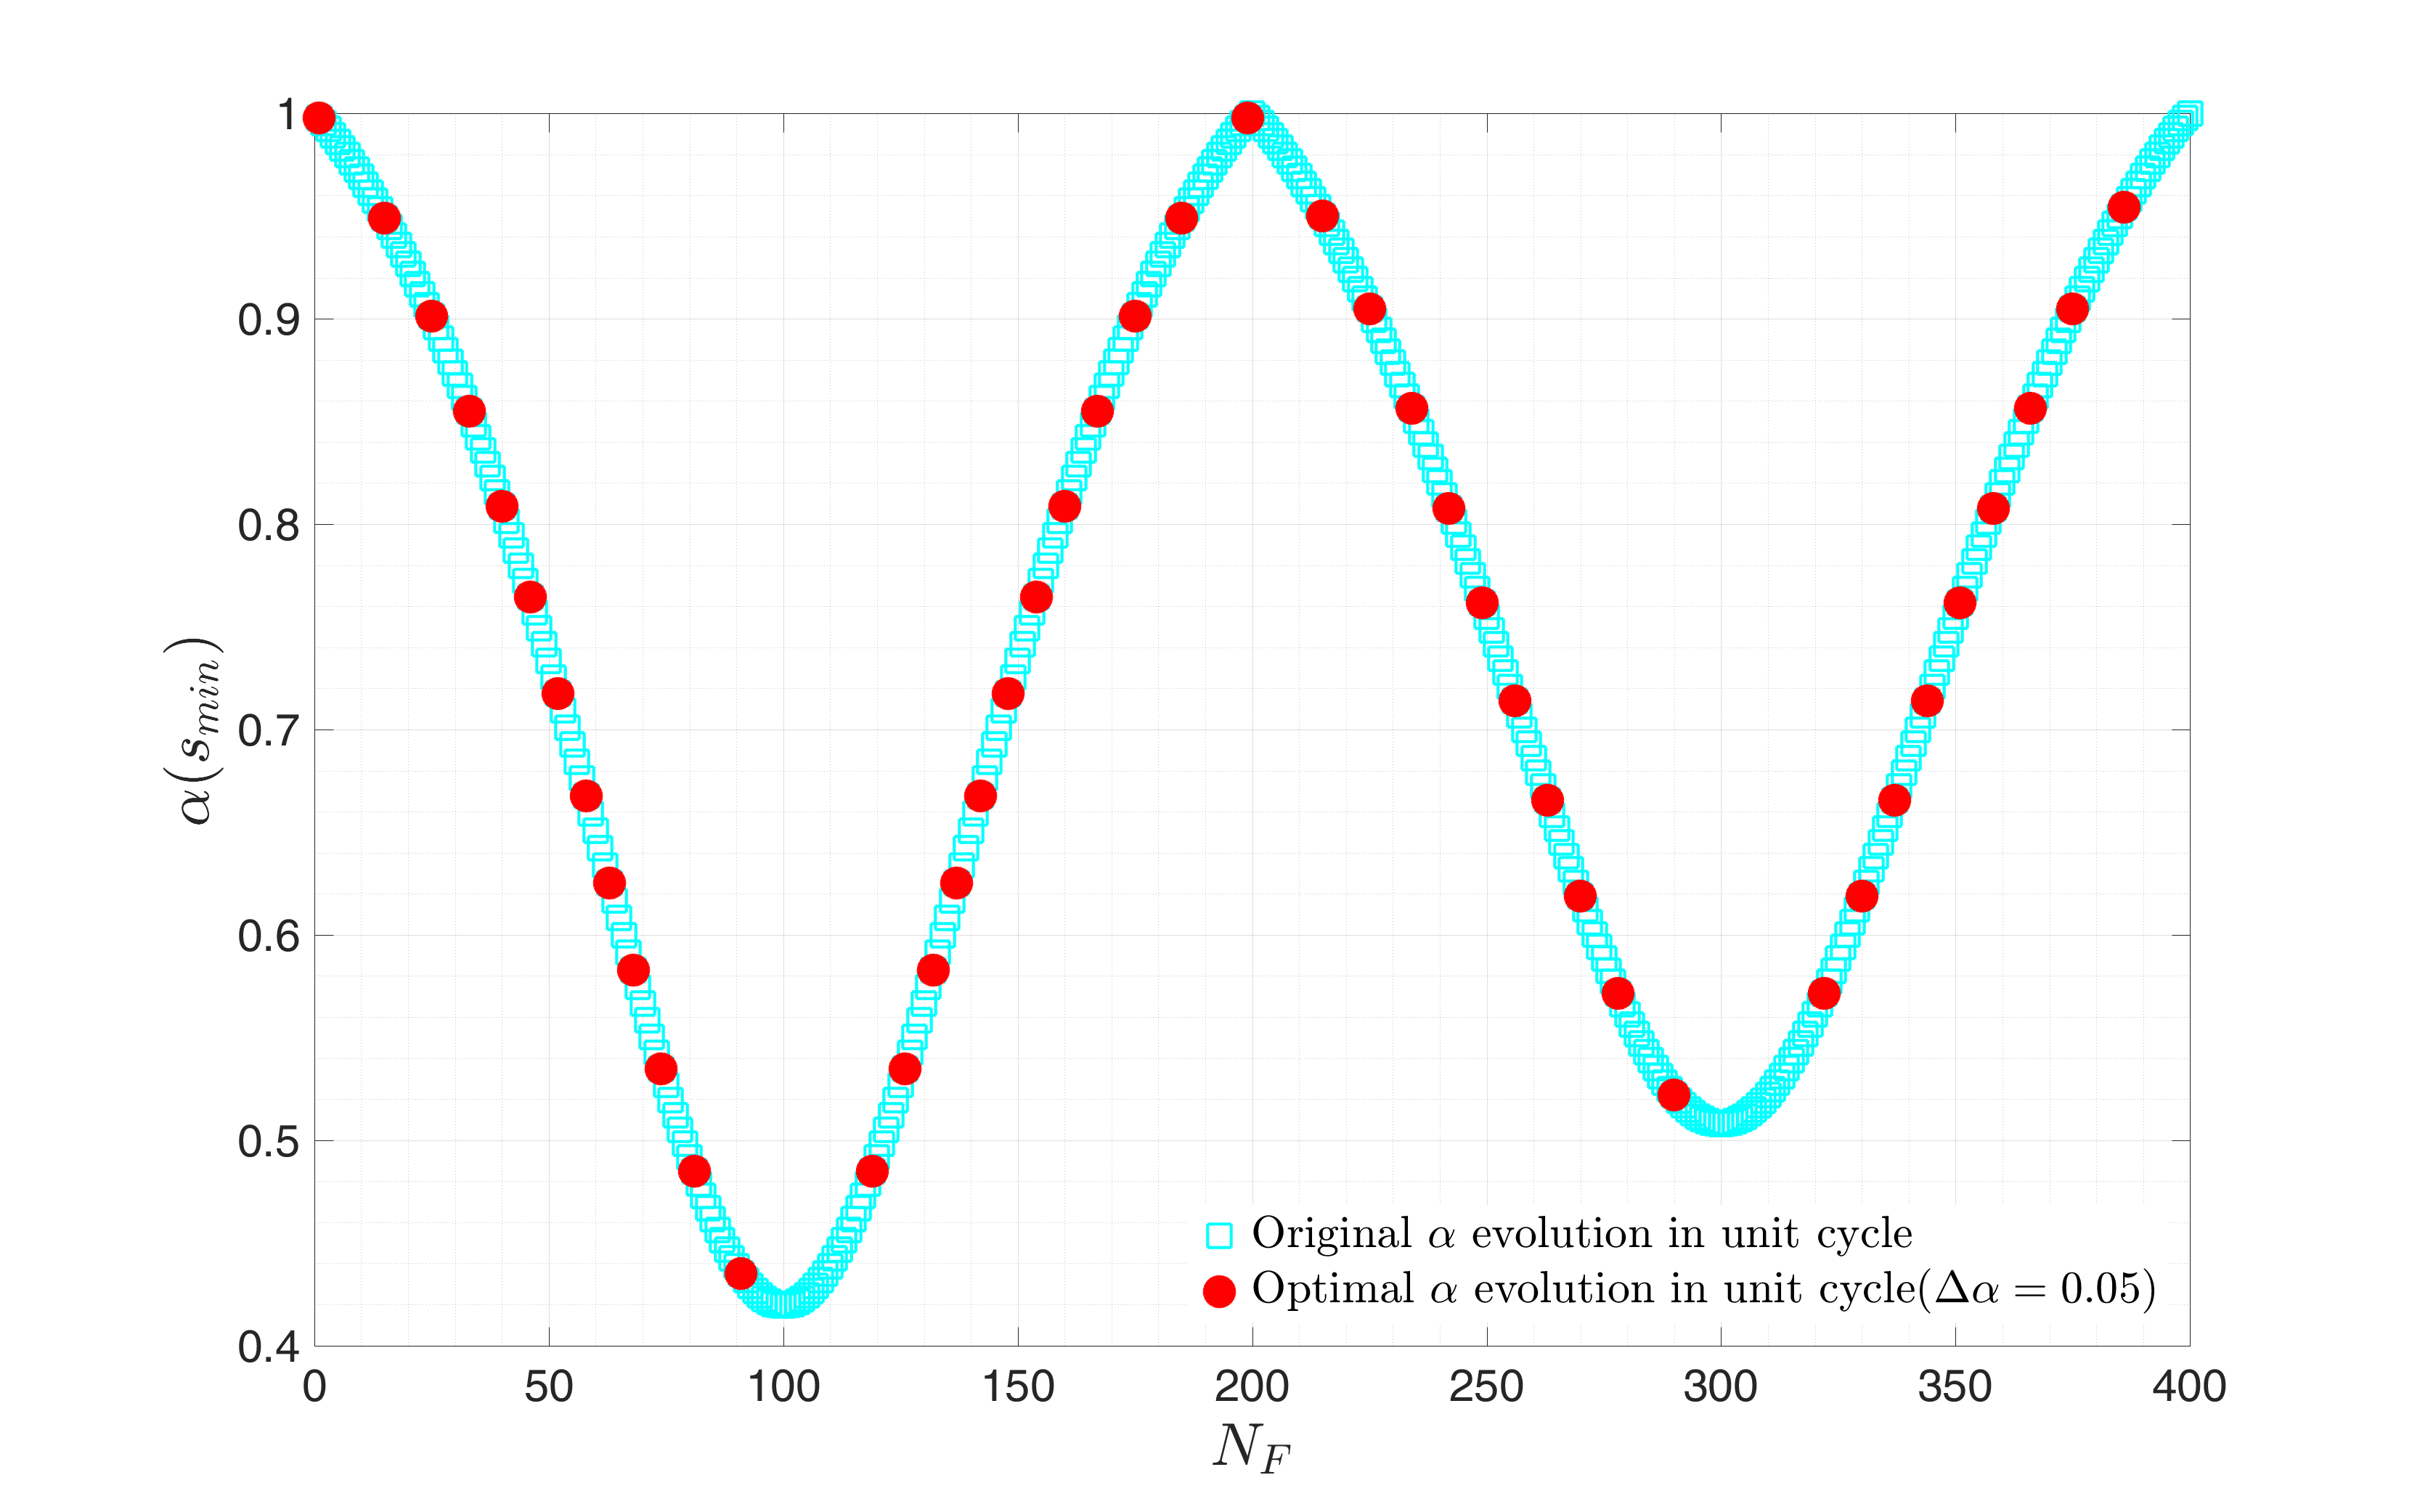
\includegraphics[width=0.8\textwidth]{figures//alpha_opt_vs_alpha_stepnumber.png} 
	\caption{Comparing numerical strategy with optimal time steps in one cycle with the old one, in this way the number of steps in unit cycle is reduced from 400 to 35, meaning a cost reduction factor of 0.0875 (with $\Delta\alpha=0.05$, $a=0.4$, $\lambda=0.1$, $\Sigma_y=230 MPa$, $\Sigma_{bending}=225 MPa$)}
	\label{fig.alpha_opt_vs_alpha_stepnumber}
\end{figure}

If $\alpha$ varies significantly, we use optimal time step numerical method to update $D$ during one time step. In more details, let us suppose that our first few cycles calculation with fine time steps $\Delta t$ has produced a sequence $\alpha(i)$ and $W_{cyc}(i)$ of exponent and dissipation at time $i\Delta t$. We then construct an adaptive time stepping strategy with variable time steps $\Delta t_{ref}(j)$, reference exponent $\alpha_{ref}(j)$ and dissipated energy $W_{ref}(j)$ by regrouping together adjacent time steps $\Delta t(i)$ with similar exponents $\alpha(i)$. This sequence is incremented as follows.


For $t_{ref}(j)$ and $\alpha_{ref}(j)=\alpha(t_{ref}(j))$ given, we set
$$\Delta t_{ref}(j)=\sum_{\substack{t(i)\geqslant t_{ref}(j)\\\left\| \alpha(i)-\alpha_{ref}(j)\right\|\leqslant \Delta\alpha }}\Delta t, \quad t_{ref}(j+1)=t_{ref}(j)+\Delta t_{ref}(j).$$
The same goes for the dissipated energy:
$$\Delta W_{ref}(j)=\sum_{\substack{t(i)\geqslant t_{ref}(j)\\\left\| \alpha(i)-\alpha_{ref}(j)\right\|\leqslant \Delta\alpha} }W_{cyc}(i) , \quad W_{ref}(j+1)=W_{ref}(j)+\Delta W_{ref}(j).$$

We finally use these new time steps with corresponding $\alpha_{ref}$ and $W_{ref}$ to update the damage by looping on all the following cycles with the new optimal time steps $j$ and cycles $N$, and updating damage in each cycle by:
\begin{equation}
D=D+D^{\alpha_{ref}(j)}\dfrac{\Delta W_{ref}(j)}{W_0},
\label{eq.optimal}
\end{equation}

with values $\alpha_{ref}(j)$ and $\Delta W_{ref}(j)$ precomputed in the first few cycles. This strategy is validated in \figref{fig.alpha_opt_vs_alpha_stepnumber}.

\vspace{6pt}
\textbf{Complexity analysis}
\vspace{6pt}

The optimal time step method clearly reduces the numerical cost. Typically, we assume the material has fatigue life of $1\times10^{6}$ cycles to failure and we implement $1000$ time steps in unit cycle. The reduction factor of points in unit cycle for example as in \figref{fig.alpha_opt_vs_alpha_stepnumber} equals $35/400=0.0875$. We can then compare the cost between full numerical strategy and the new one.

\begin{table}[!h]
\centering
\begin{tabular}{l|l}
\hline
Full numerical strategy: & $1000$ time steps $\times$ $64$ scales $\times$  $1\times10^{6}$ cycles       \\ \hline
Optimal cyclic strategy: & \begin{tabular}[l]{@{}l@{}} $1000$ time steps $\times$ $64$ scales $\times$  $5$ cycles until stabilization  \\$+$ $1\times10^{6}$ cycles $\times$ ($1000$ time steps $\times$ reduction factor)      \end{tabular}  \\ \hline
Ratio between optimal and full: & $\approx \dfrac{reduction \; factor}{64 \; scales}=\dfrac{1}{731}$       \\ \hline
\end{tabular}
\end{table}

The same strategy is applied to random loading situations which are made of repeated sequence of random loads:

\begin{itemize}
	\item calculation of dissipated energy and exponent on one sequence;
	
	\vspace{6pt}	
	
	\item time coarsening;
	
	\vspace{6pt}	
	
	\item repeated integration of damage through the different sequences.
		
	\vspace{6pt}
\end{itemize}
                          
In such a strategy, the extra cost of introducing multiple scales in the calculation becomes negligible as compared to the time integration of damage in the evolution process.

\begin{Figure}[]{S-N curve of bending test on 30NCD16 steel using numerical and analytical method (Eq.\eqref{eq.cycNF}) with different time steps. Data are those of table.\ref{tab:Sin}}[fig.sn-num-ana]
	\centerline{
		\graphfile*[38]{figures//SN_num_ana_stepnumber=30.png}[30 time steps in unit cycle($\beta=1.1$, $a=0.001$).]
		\graphfile*[38]{figures//SN_num_ana_stepnumber=100.png}[100 time steps in unit cycle($\beta=1.1$, $a=0.001$).]}
	\\
	\centerline{
		\graphfile*[38]{figures//SN_num_ana_stepnumber=30_err.png}[Relative error$\left( \dfrac{NF_{num}-NF_{analytical}}{NF_{analytical}}\right)$  with 30 time \protect \\ steps in unit cycle  ($\beta=1.1$, $a=0.001$)]
		\graphfile*[38]{figures//SN_num_ana_stepnumber=100_err.png}[Relative error$\left( \dfrac{NF_{num}-NF_{analytical}}{NF_{analytical}}\right)$   with 100 time \protect \\ steps in unit cycle  ($\beta=1.1$, $a=0.001$)]}
	\label{fig.sn-num-ana}
\end{Figure}

\newpage

Altogether, we have three numerical approaches for integrating damage.

\begin{enumerate}
	\item  Numerical results with varying $\alpha$(equally divide time in unit cycle), and do the scale integration all along the fatigue life time, which can be of high numerical cost$$\delta D=D^\alpha\frac{\dot{W}}{W_0}\delta t.$$
	This method only serves for qualification purposes.
	\vspace{6pt}
	
	\item  Numerical results with optimal time steps(equally divide $\alpha$in unit cycle), here we have $\Delta\alpha=0.01$, to reduce time steps needed, after several cycles adaptation we iterate using the recorded scalar values of $\alpha_{ref}$, $W_{ref}$ and $t_{ref}$ to decide fatigue life time.
	$$\delta D=D^{\alpha_{ref}}\frac{W_{ref}}{W_0}\delta t_{ref}.$$
	\vspace{6pt}
	
	\item  Analytical results after integration of D (with mean alpha from numerical strategy)$$N_F=\frac{W_0}{( 1-\alpha_m)W_{cyc}},$$ 
	which is derived from the differential equation
	$$\delta D=D^{\alpha_m}\frac{W_{cyc}}{W_0}\delta N.$$
\end{enumerate}	

Although method 2 is much more numerically efficient than the original numerical method 1, it is still not cheap in the experimental fitting process. We need the analytical formula method 3 to do the fitting process. To validate the feasibility, we now compare only the analytical(method 3) one and optimal time steps(method 2) one. The results are shown in \figref{fig.SNnumerical2methods} and \figref{fig.SNnumerical2methods2}, the relation ship between relative error and $\Delta \alpha$ with 2000 time steps in unit cycle is shown in  \figref{fig.errorNumAna0.02} and \figref{fig.errorNumAna0.01}.
\begin{figure}[!h]
	\centering
	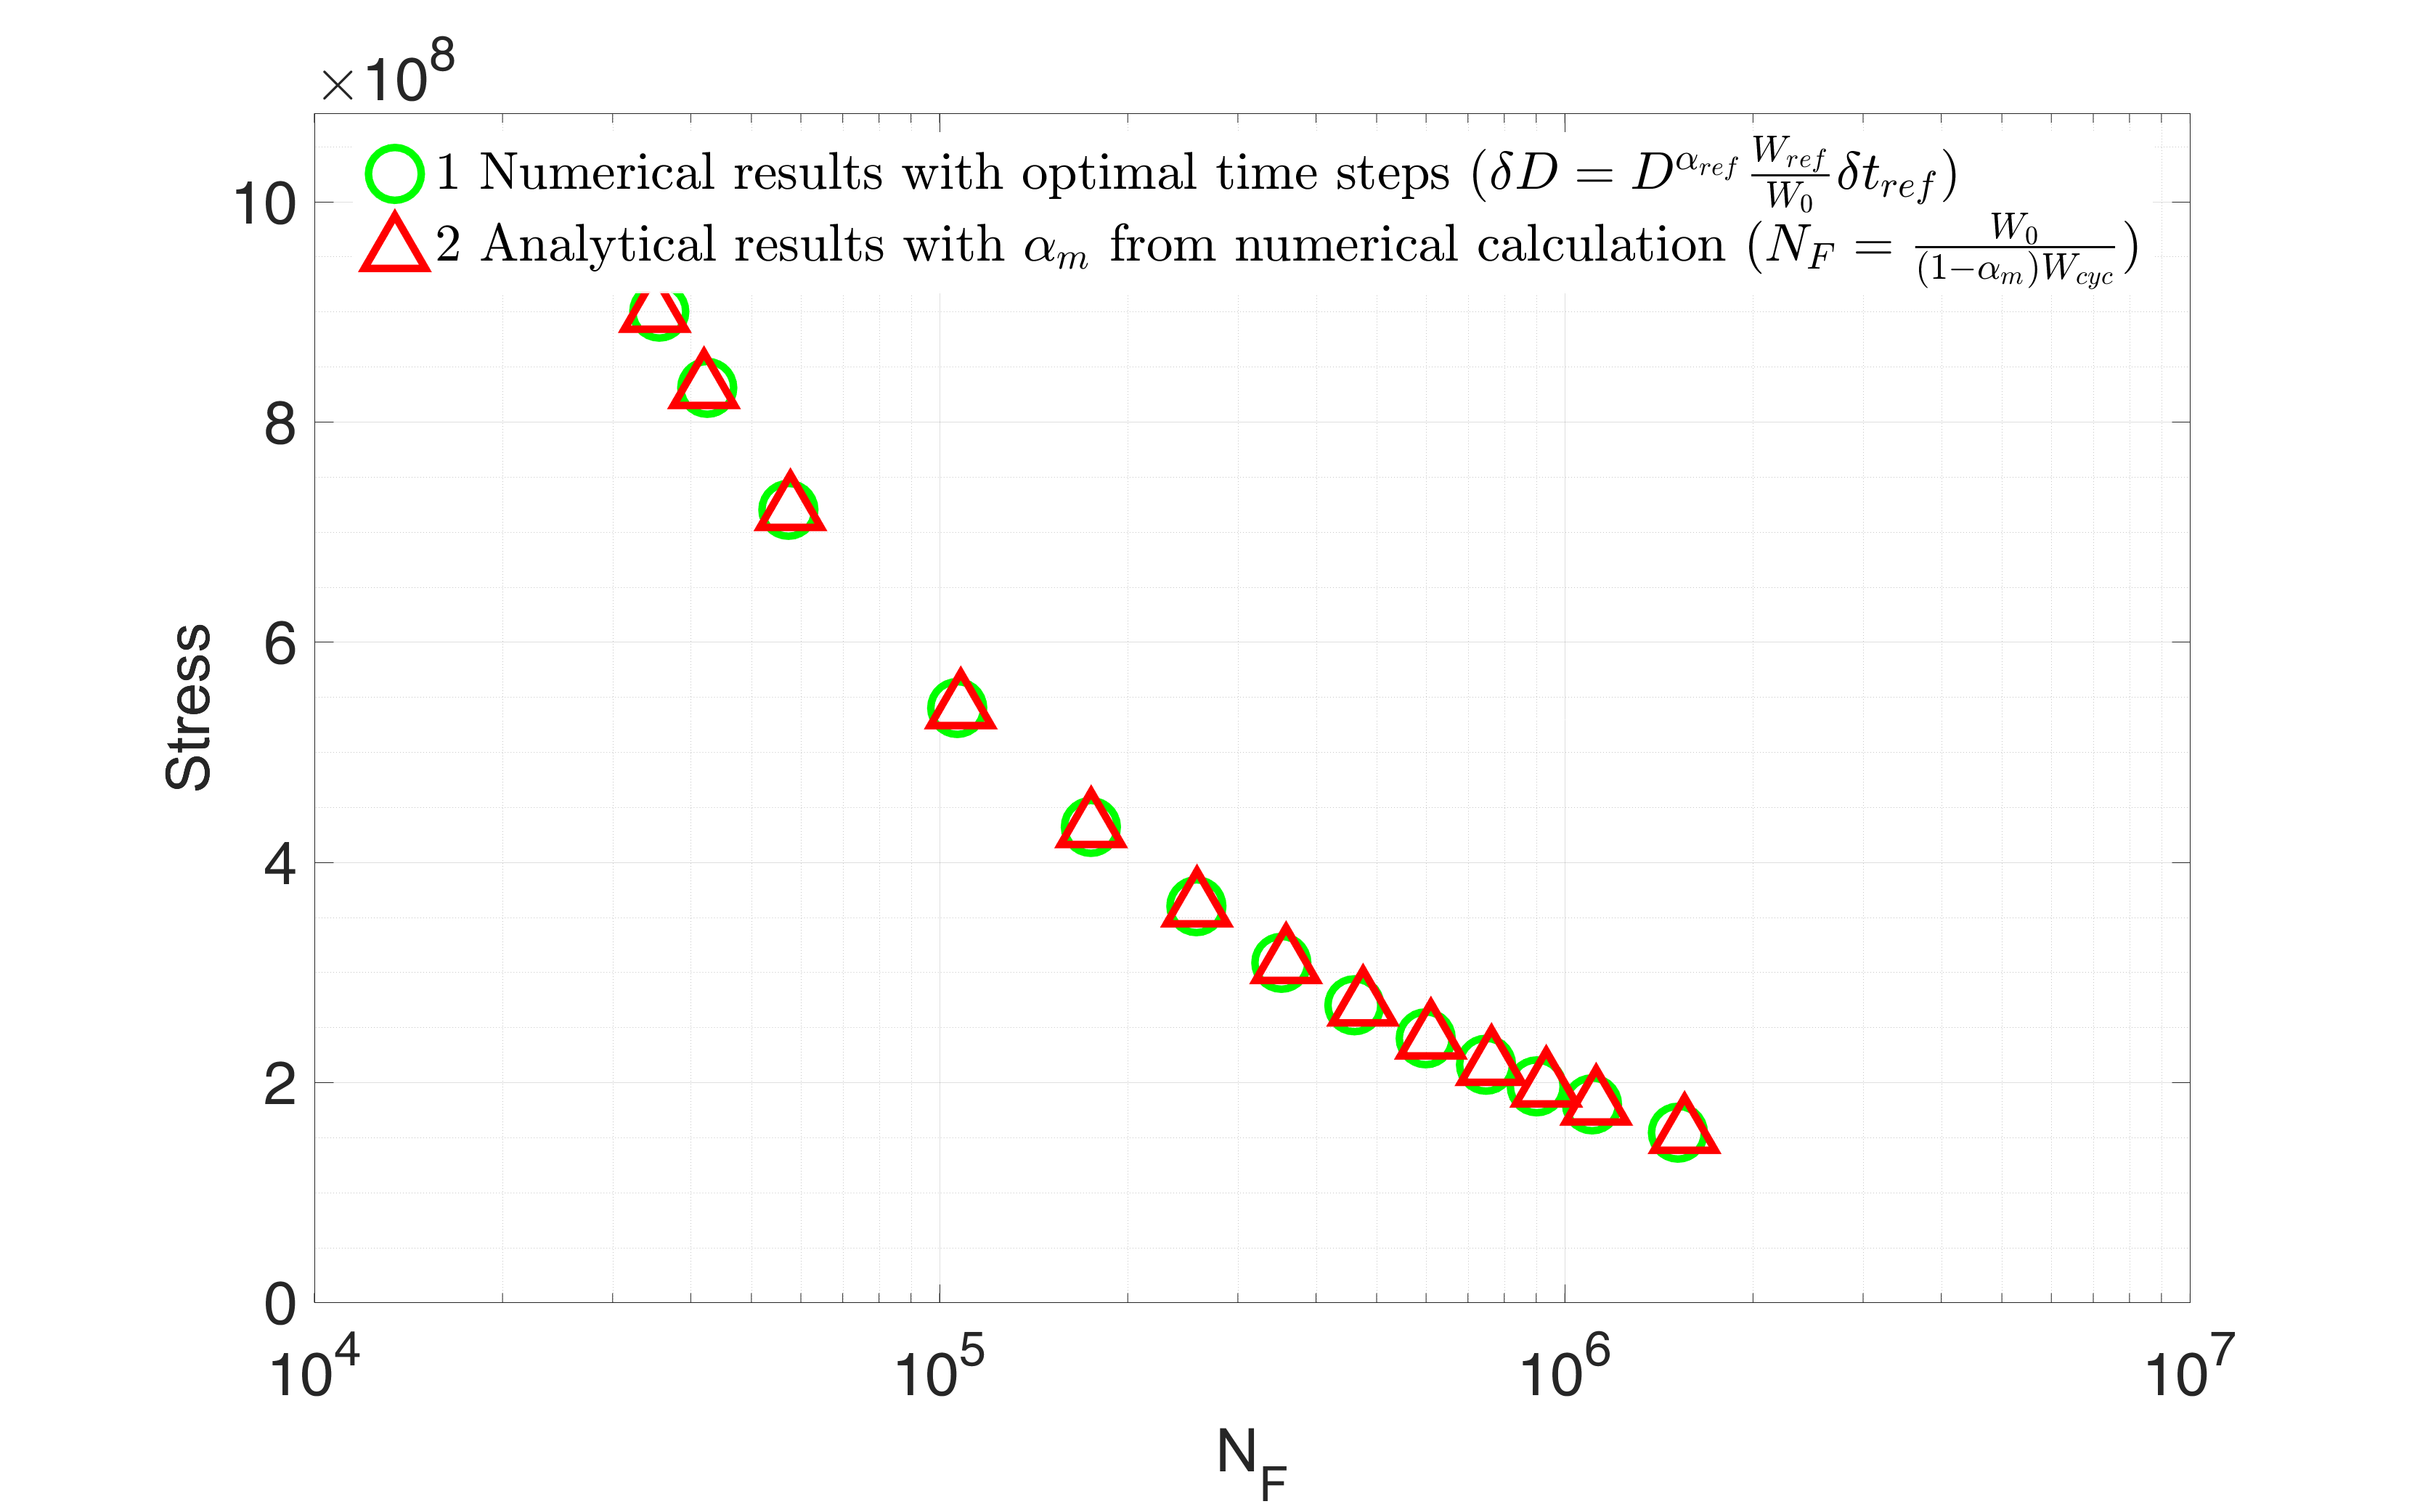
\includegraphics[width=\textwidth]{figures//SN_opt_ana_200_delta_alp=0.00002.png} 
	\caption{S-N curve using analytical and numerical results with optimal time steps methods ($\beta=1.1$, $a=0.01$, $\Delta \alpha=2E-5$ in unit cycle), yielding 200 full time steps reduced to 197 optimal time steps}
	\label{fig.SNnumerical2methods}
\end{figure}
\begin{figure}[!h]
	\centering
	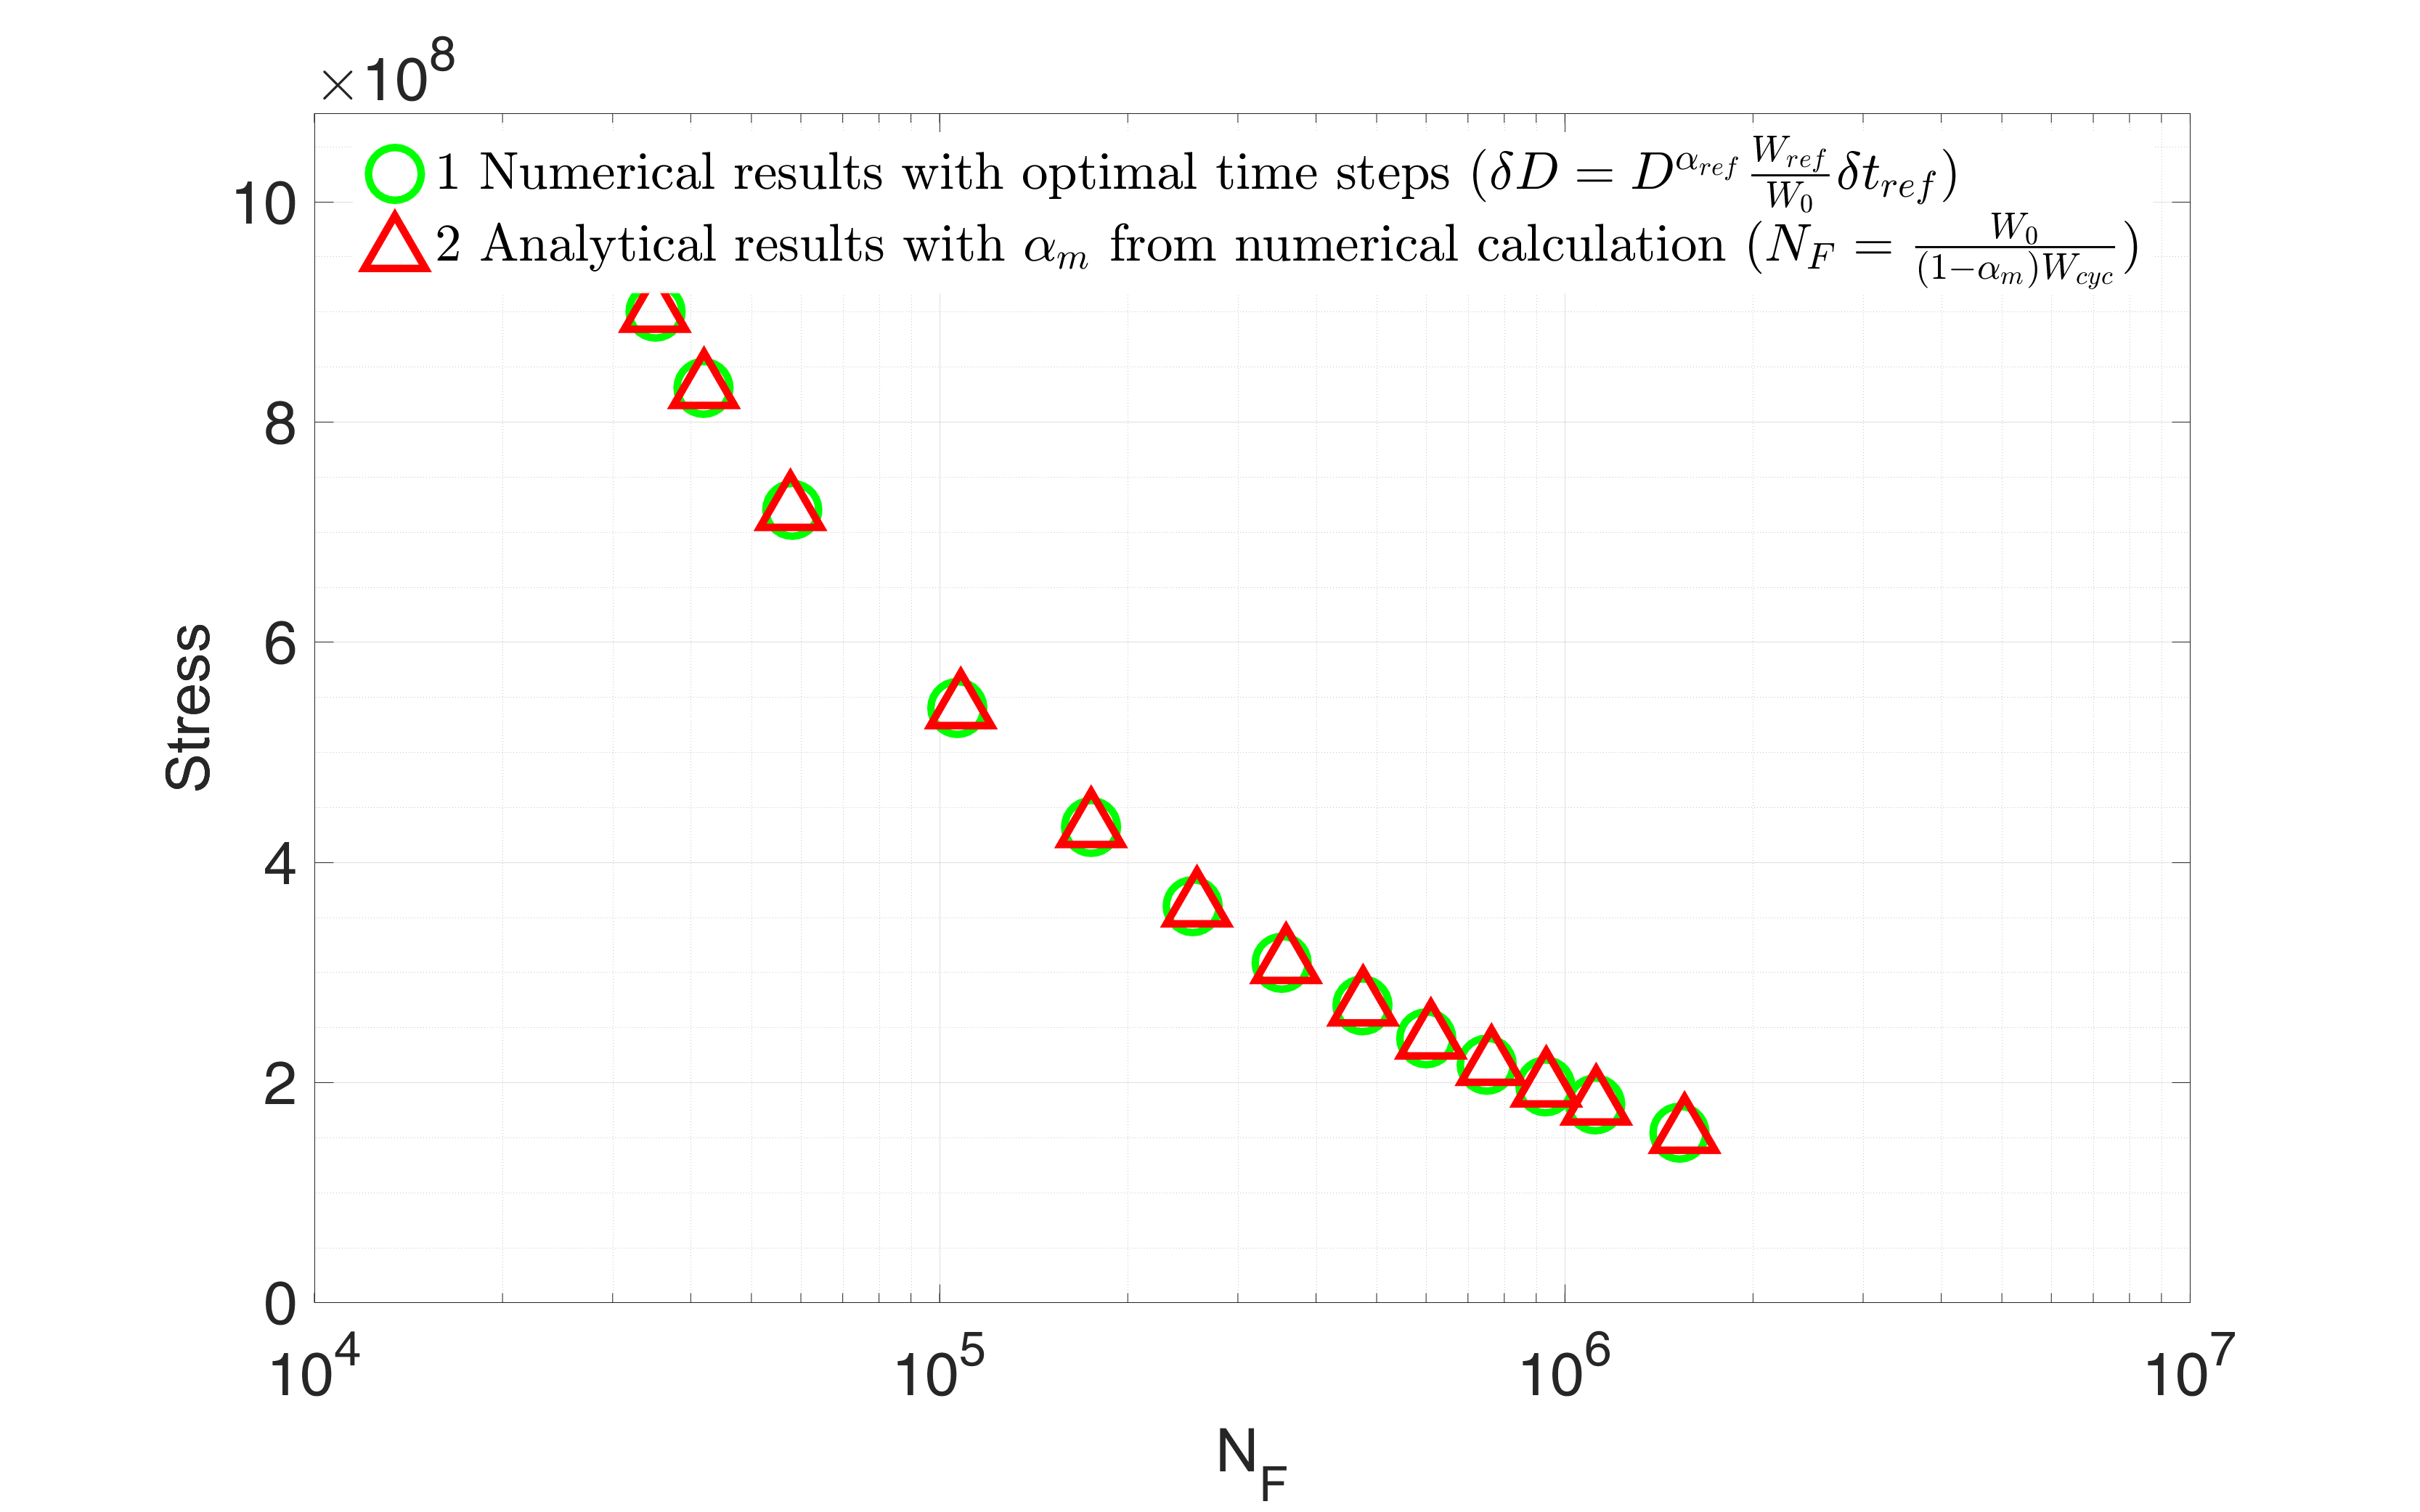
\includegraphics[width=\textwidth]{figures//SN_opt_ana_200_delta_alp=0.00001.png} 
	\caption{S-N curve using analytical and numerical results with optimal time steps methods ($\beta=1.1$, $a=0.01$, $\Delta \alpha=1E-5$ in unit cycle), yielding 200 full time steps reduced to 199 optimal time steps}
	\label{fig.SNnumerical2methods2}
\end{figure}
\begin{figure}[!h]
	\centering
	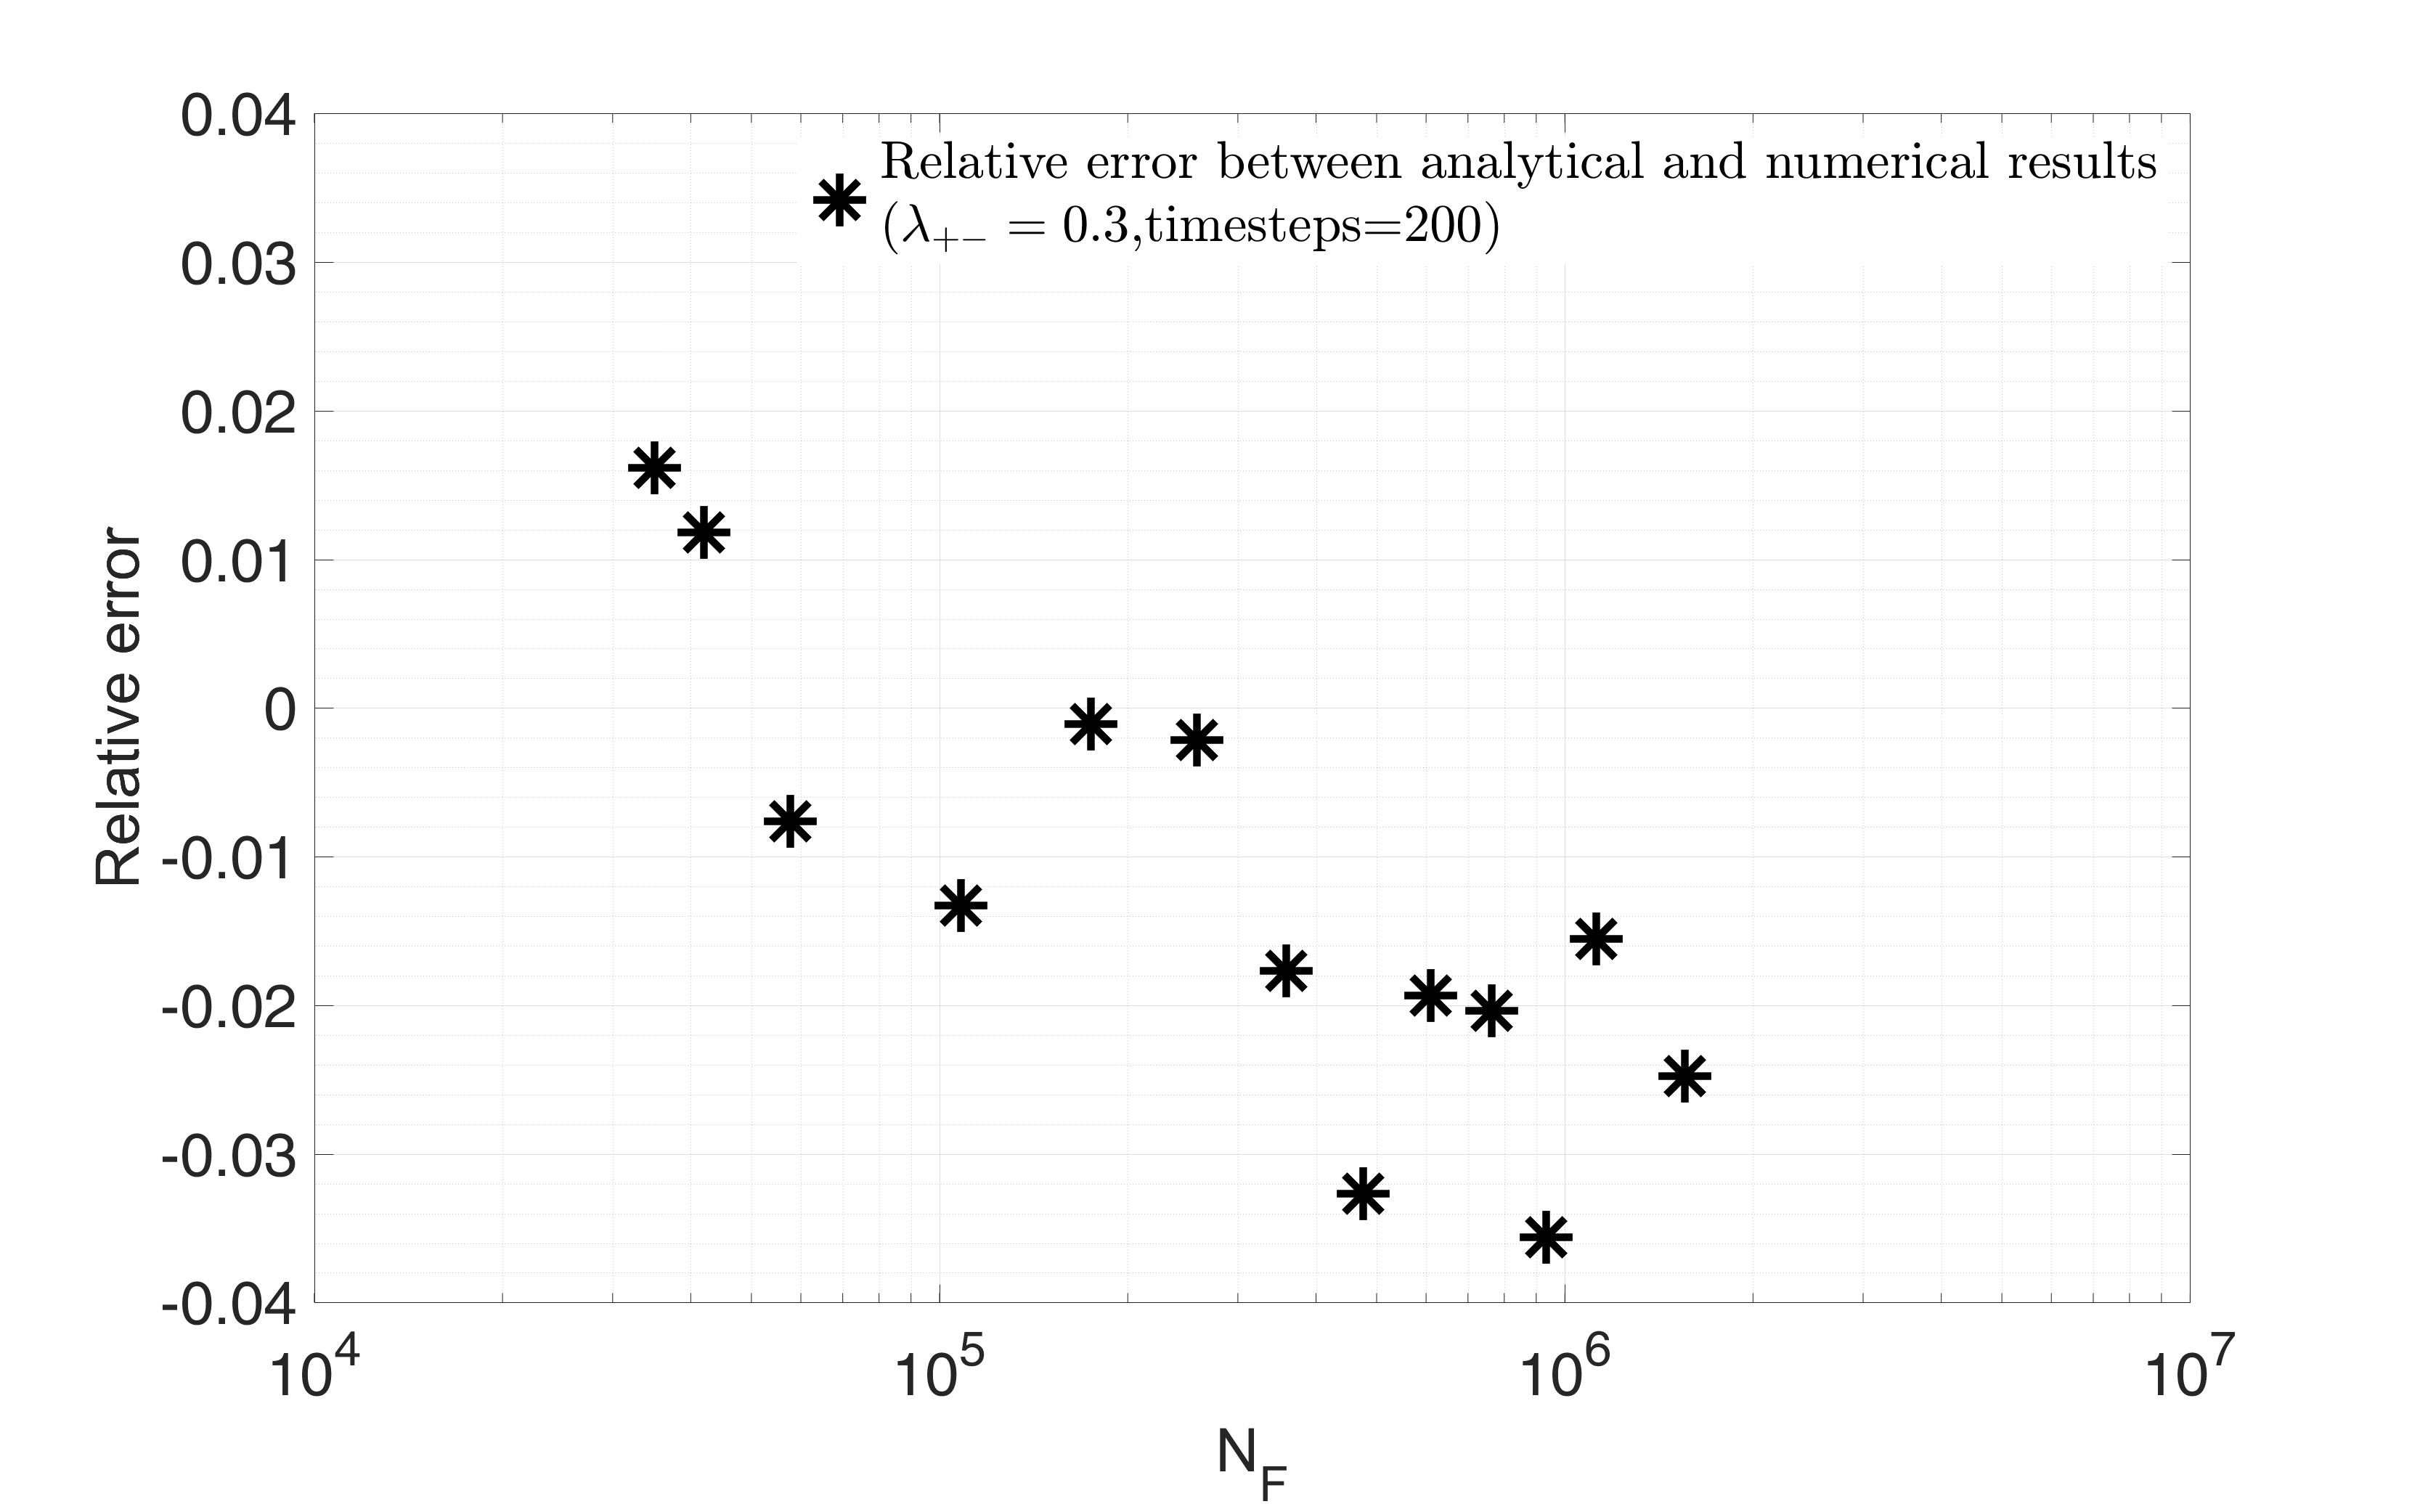
\includegraphics[width=\textwidth]{figures//SN_opt_ana_200_delta_alp=0.00002_err.png} 
	\caption{Relative error $\left( \dfrac{NF_{opt}-NF_{analytical}}{NF_{analytical}}\right)$  between analytical and numerical results with optimal time steps methods ($\beta=1.1$, $a=0.01$, $\Delta \alpha=2\times10^{-5}$ in unit cycle)}	
	\label{fig.errorNumAna0.02}
\end{figure}
\begin{figure}[!h]
	\centering
	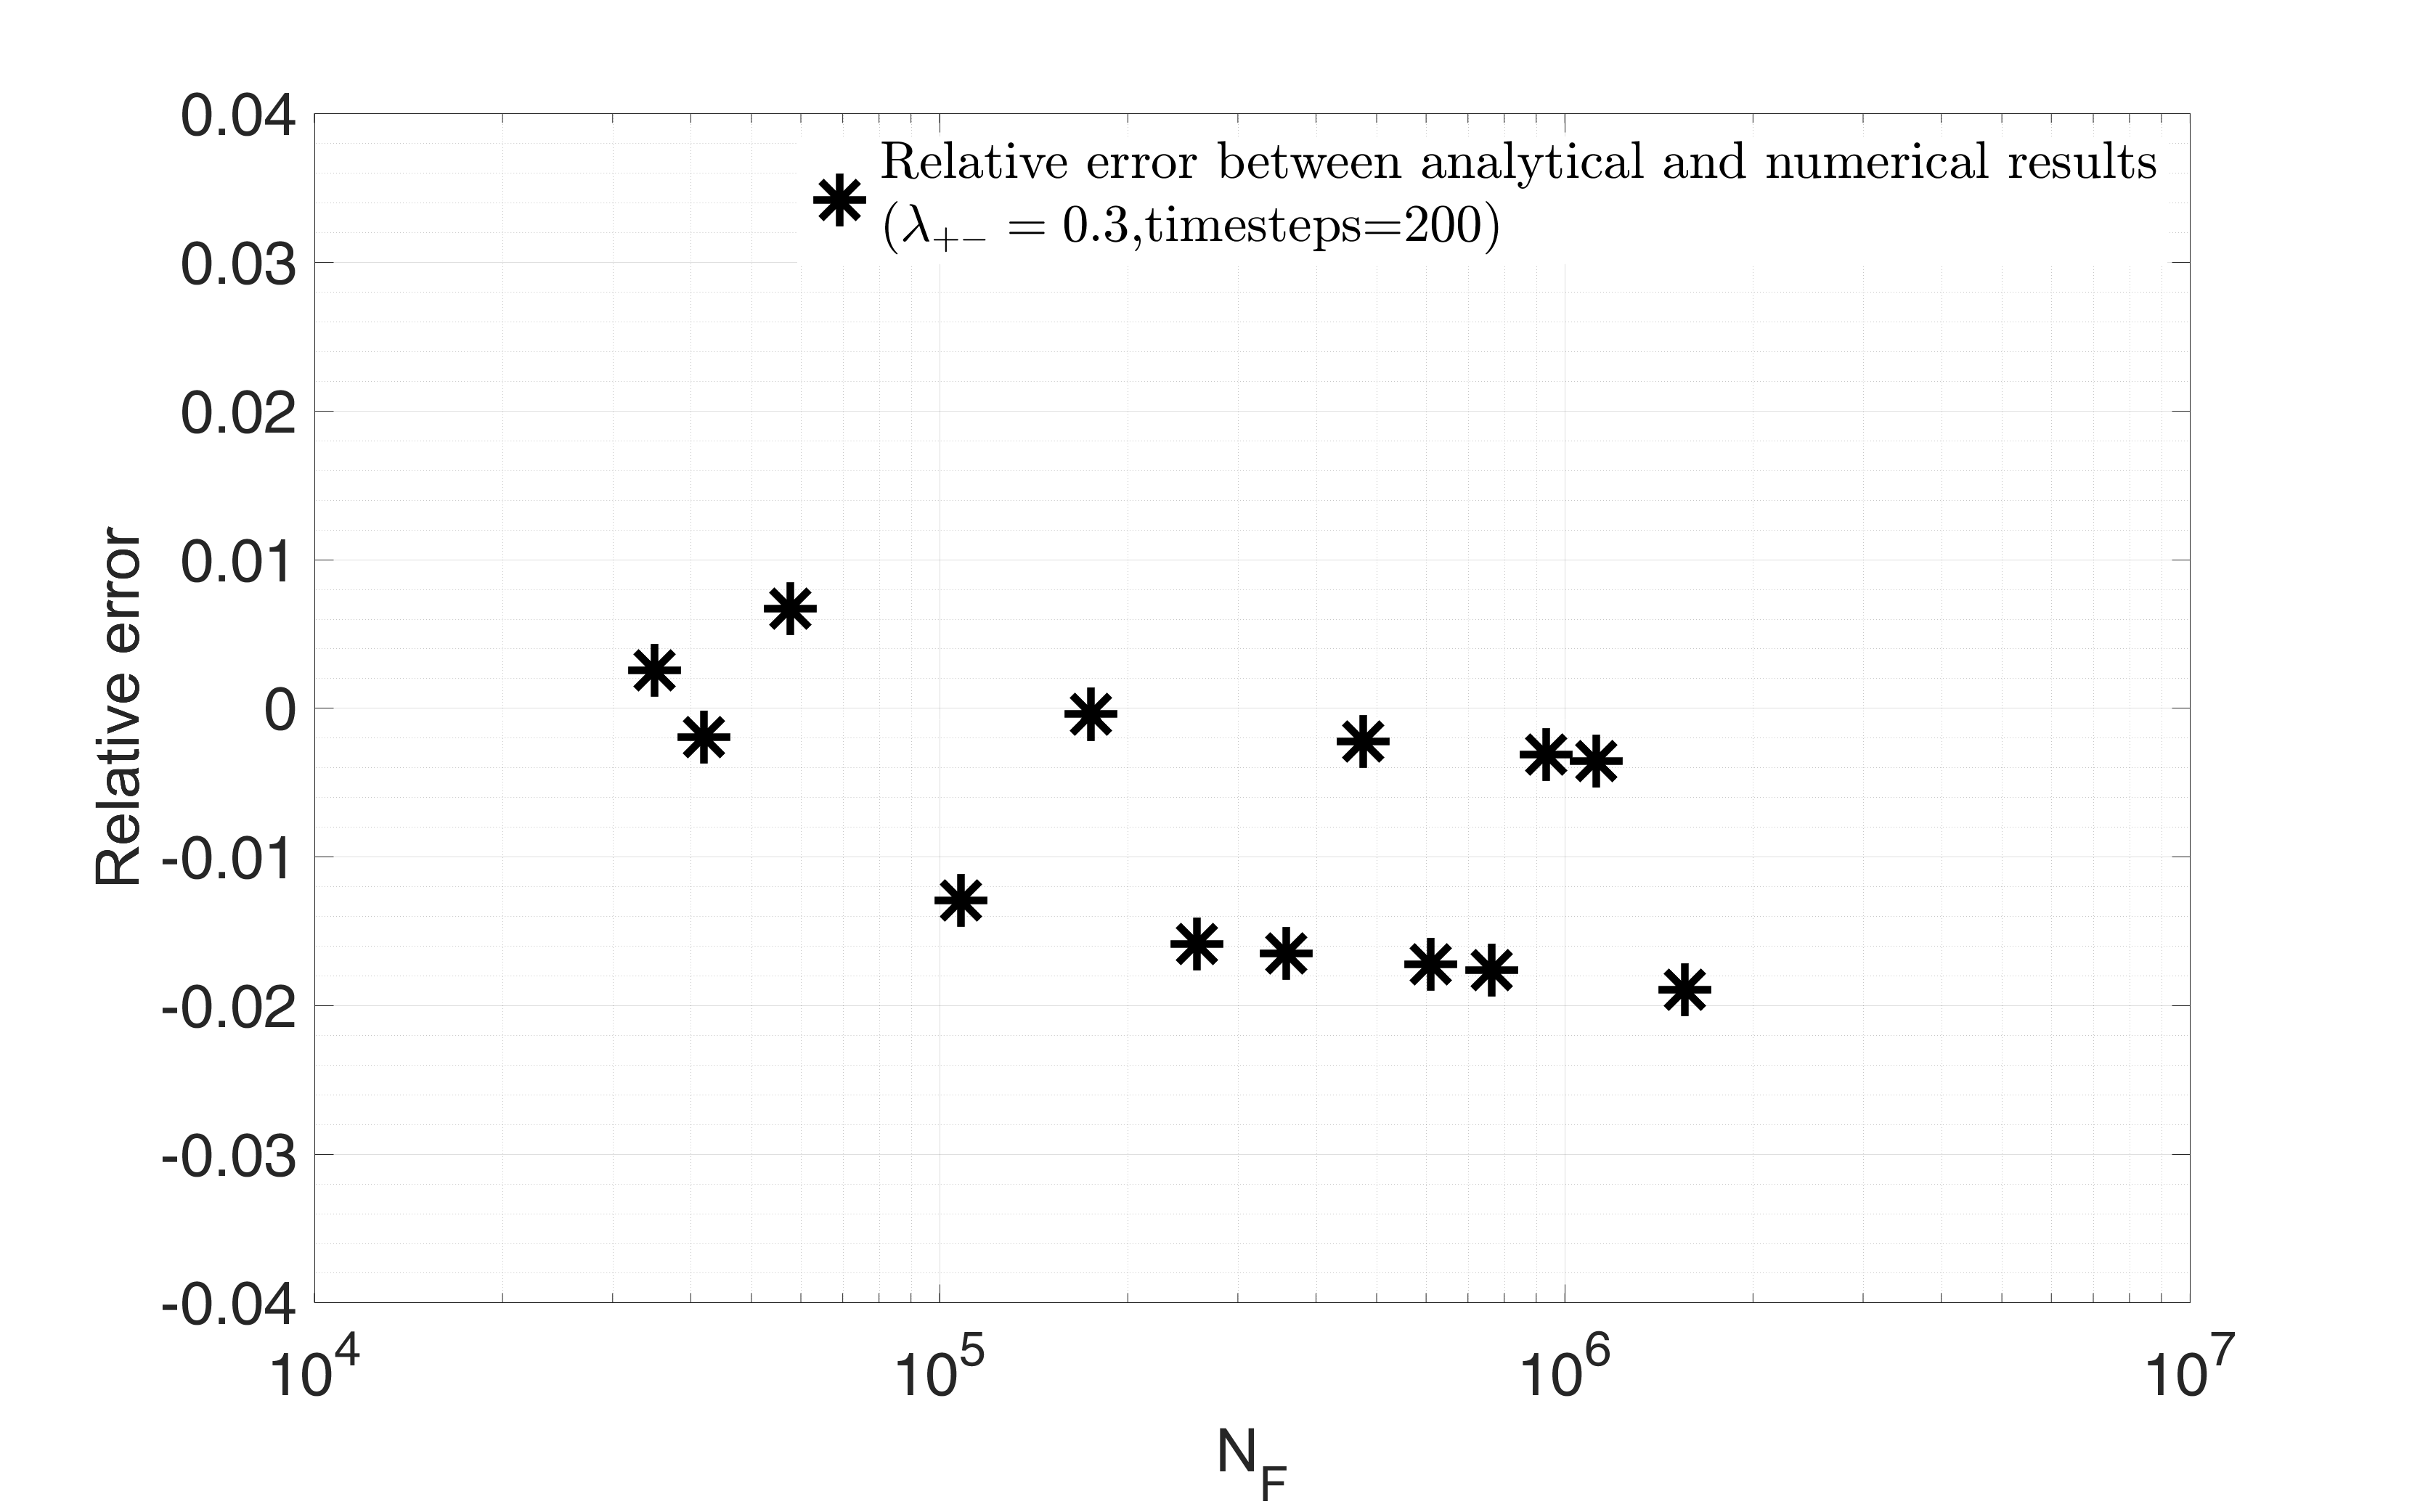
\includegraphics[width=\textwidth]{figures//SN_opt_ana_200_delta_alp=0.00001_err.png} 
	\caption{Relative error $\left(\dfrac{NF_{opt}-NF_{analytical}}{NF_{analytical}}\right)$  between analytical and numerical results with optimal time steps methods ($\beta=1.1$, $a=0.01$, $\Delta \alpha=1\times10^{-5}$ in unit cycle)}
	\label{fig.errorNumAna0.01}
\end{figure}

Now we can conclude that with more time steps in unit cycle, we get closer results with the original numerical method(method 2) in HCF regime. With smaller $\Delta \alpha$ value, we get less relative error between numerical(method 3) and analytical(method 1) results. This indicates that in constant amplitude cyclic loading, with moderate values of $\beta$ it is feasible to use the analytical formula, given $\alpha_m$ is calculated using sufficient large time steps and small $\Delta \alpha$ in the first several cycles.

\clearpage
\section{Validation on recovery tests}
\label{sec:5.8}
\subsection{Recovery of Chaboche law on cyclic loading}
The test is first performed on a sinusoidal uniaxial load $\Sigma_{11}(t)=Asin(t)$, giving a deviatoric amplitude$S_{a}(t)=\sqrt{J_{2,a}(dev\uuline{\Sigma(t)})}$  so that $S_{a}(t)=\left\| \sqrt{\dfrac{1}{3}}\Sigma_{11}(t)\right\| $. We use parameters in Table.\ref{tab:Sin} to recover the classic Chaboche law in cyclic loading.
\begin{table}[!h]
	\centering
	\begin{tabular}{ll}
		\hline
		\textbf{Parameters}                                         & \textbf{Value}                    \\ \hline
		Young's modulus                                             & $E=191$ GPa                       \\
		Hardening parameter                                         &  $k=1$ GPa \\
		Weakening scales distribution exponent                      & $\beta=1.5$                             \\
		Hydrostatic pressure sensitivity                            & $\lambda_{+-}=0.6$                     \\
		Macroscopic yield stress                                    & $\sigma_y=1080$ MPa              \\
		Sequencing effect sensitivity                               & $a=0.1$                        \\
		Dissipated energy to failure per unit volume                & $W_0=5$ MJ(MPa)                       \\ \hline
	\end{tabular}
	\caption{Material parameters in a simple cyclic load }
	\label{tab:Sin}
\end{table}

We use matlab to numerically realize our method. The plot of $\left\|  \uline{\uline{S}}-\uline{\uline{b}}\right\|_{trial}$ and $\left\|  \uline{\uline{S}}-\uline{\uline{b}}\right\|$ during the first cycles at two different scales($s_{3}=1.21$ and $s_{10}=1.13$) are shown in \figref{fig.trialsin0} and \figref{fig.trialsinm}. We use here a fixed value of $\lambda$($\lambda_+=\lambda_-$), thus the local yield limit is reduced in traction and increased
in compression.

\begin{figure}[!h]
	\centering
	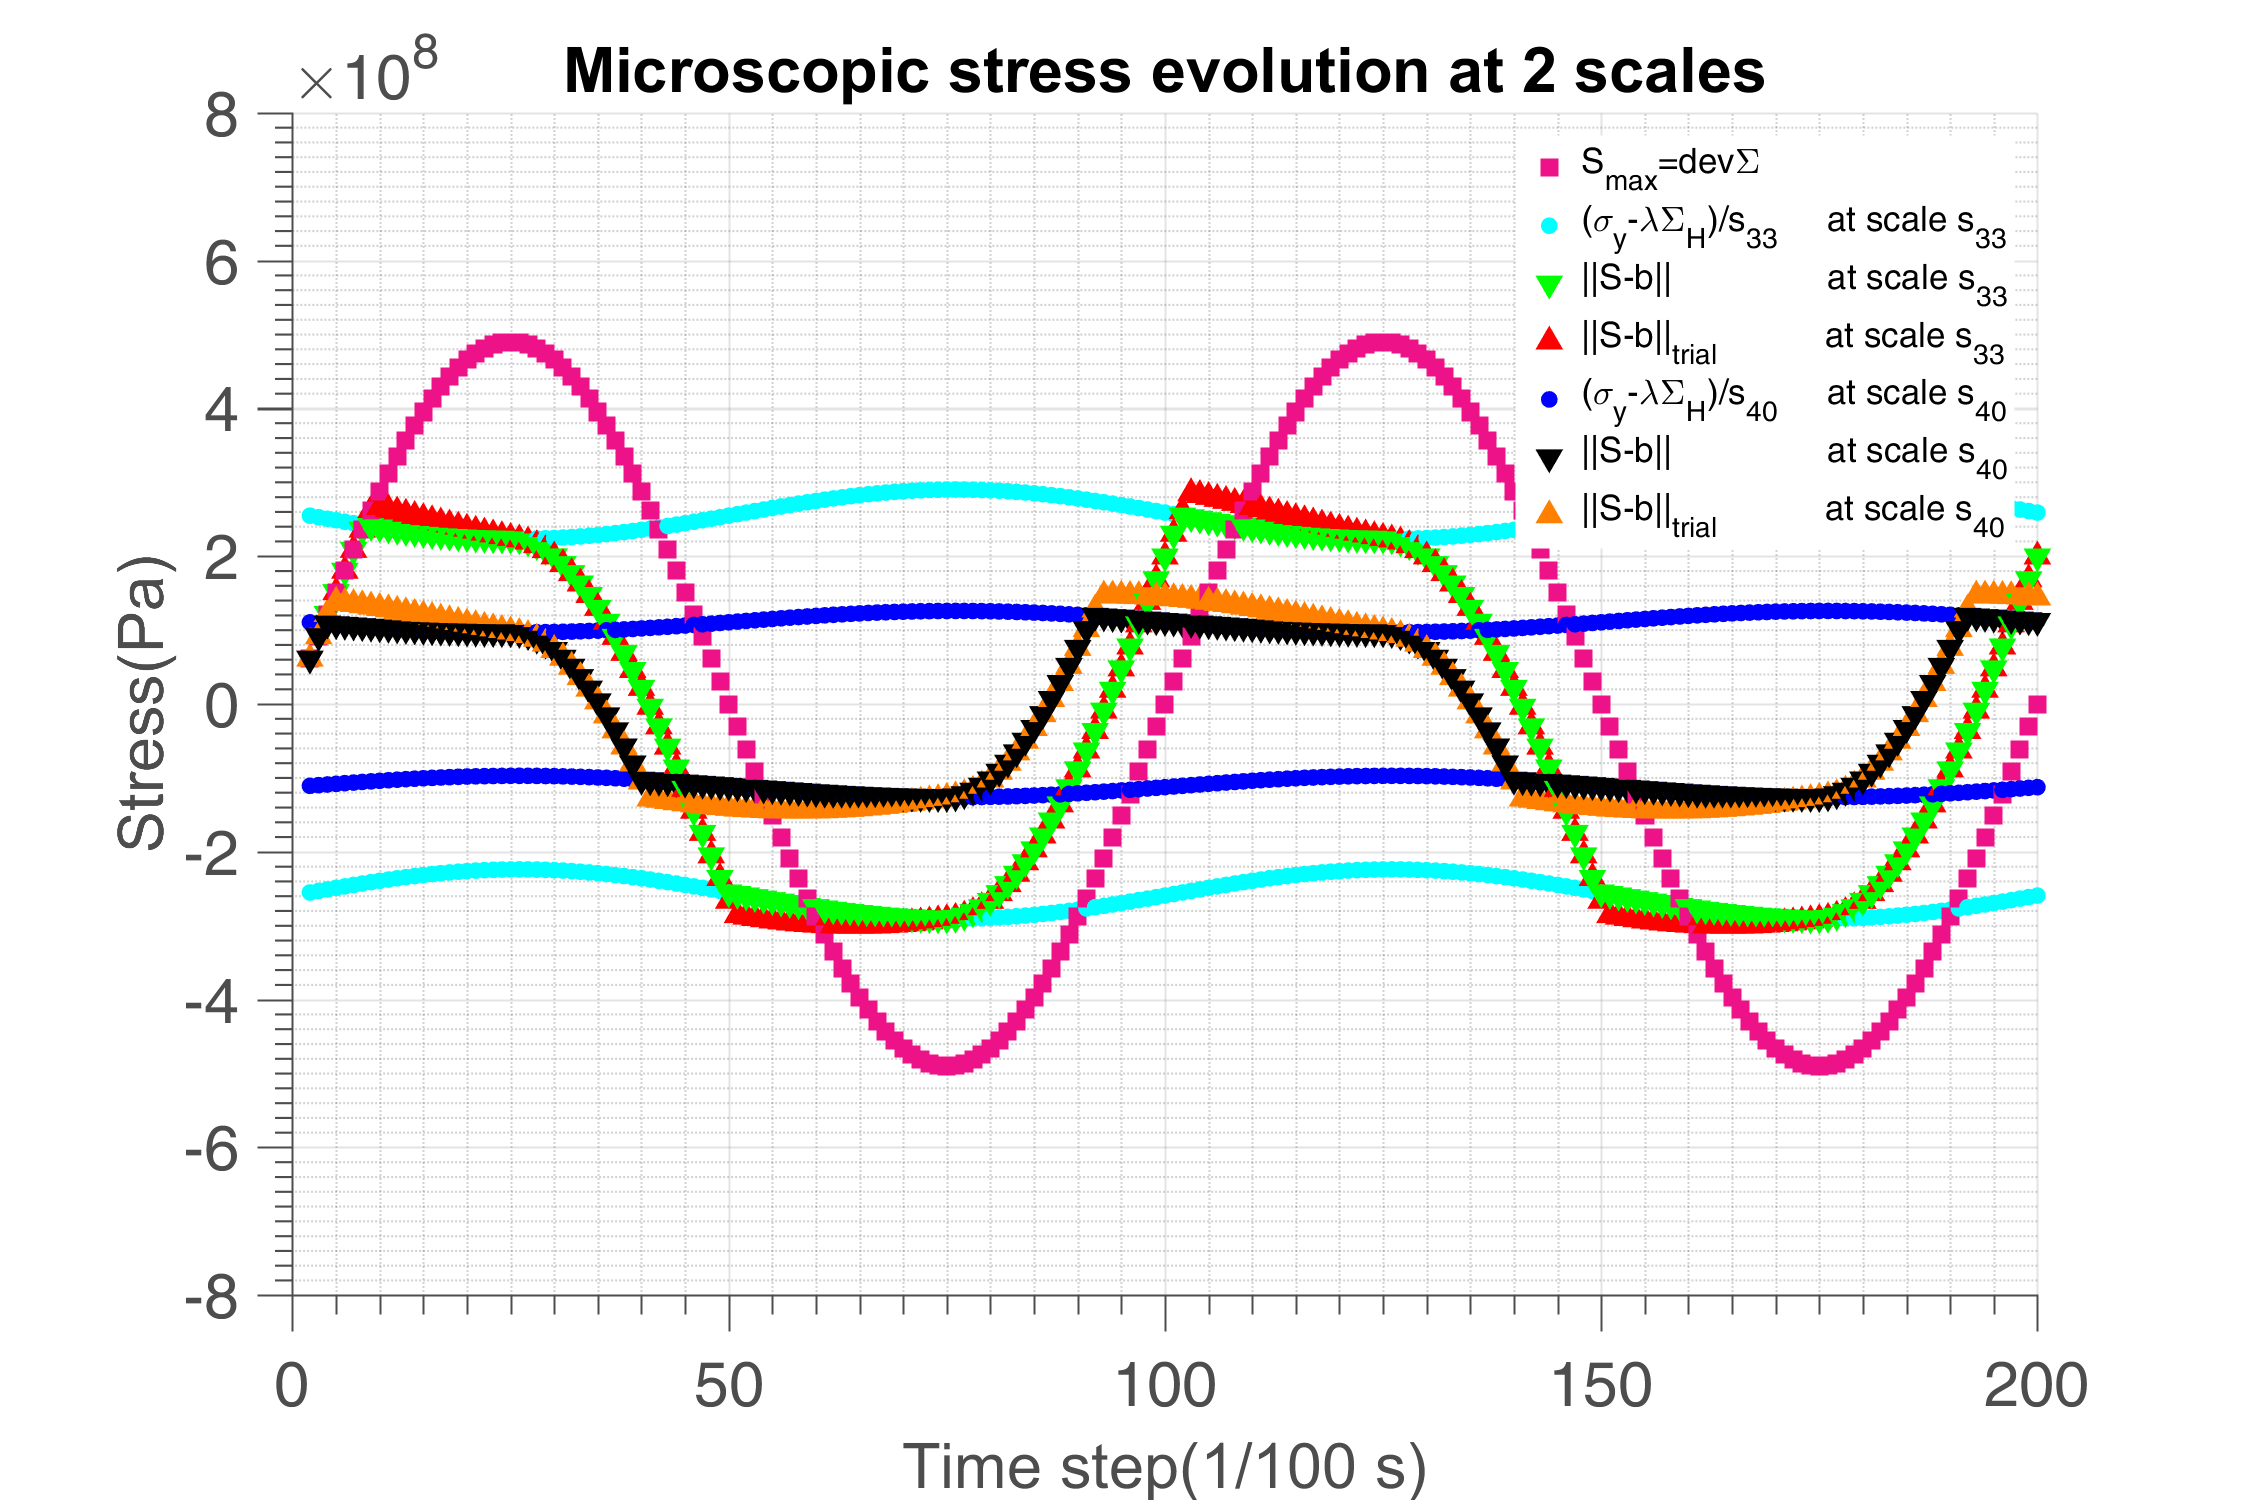
\includegraphics[width=\textwidth]{figures//trialsin_0.png} 
	\caption{Microscopic $\left(  \uline{\uline{S}}-\uline{\uline{b}}\right)_{trial}$ and $\left( \uline{\uline{S}}-\uline{\uline{b}}\right)$ evolution with time under different weakening scales($s_{3}=1.21$ and $s_{10}=1.13$) in sinusoidal load with zero mean stress}
	\label{fig.trialsin0}
\end{figure}
\begin{figure}[!h]
	\centering
	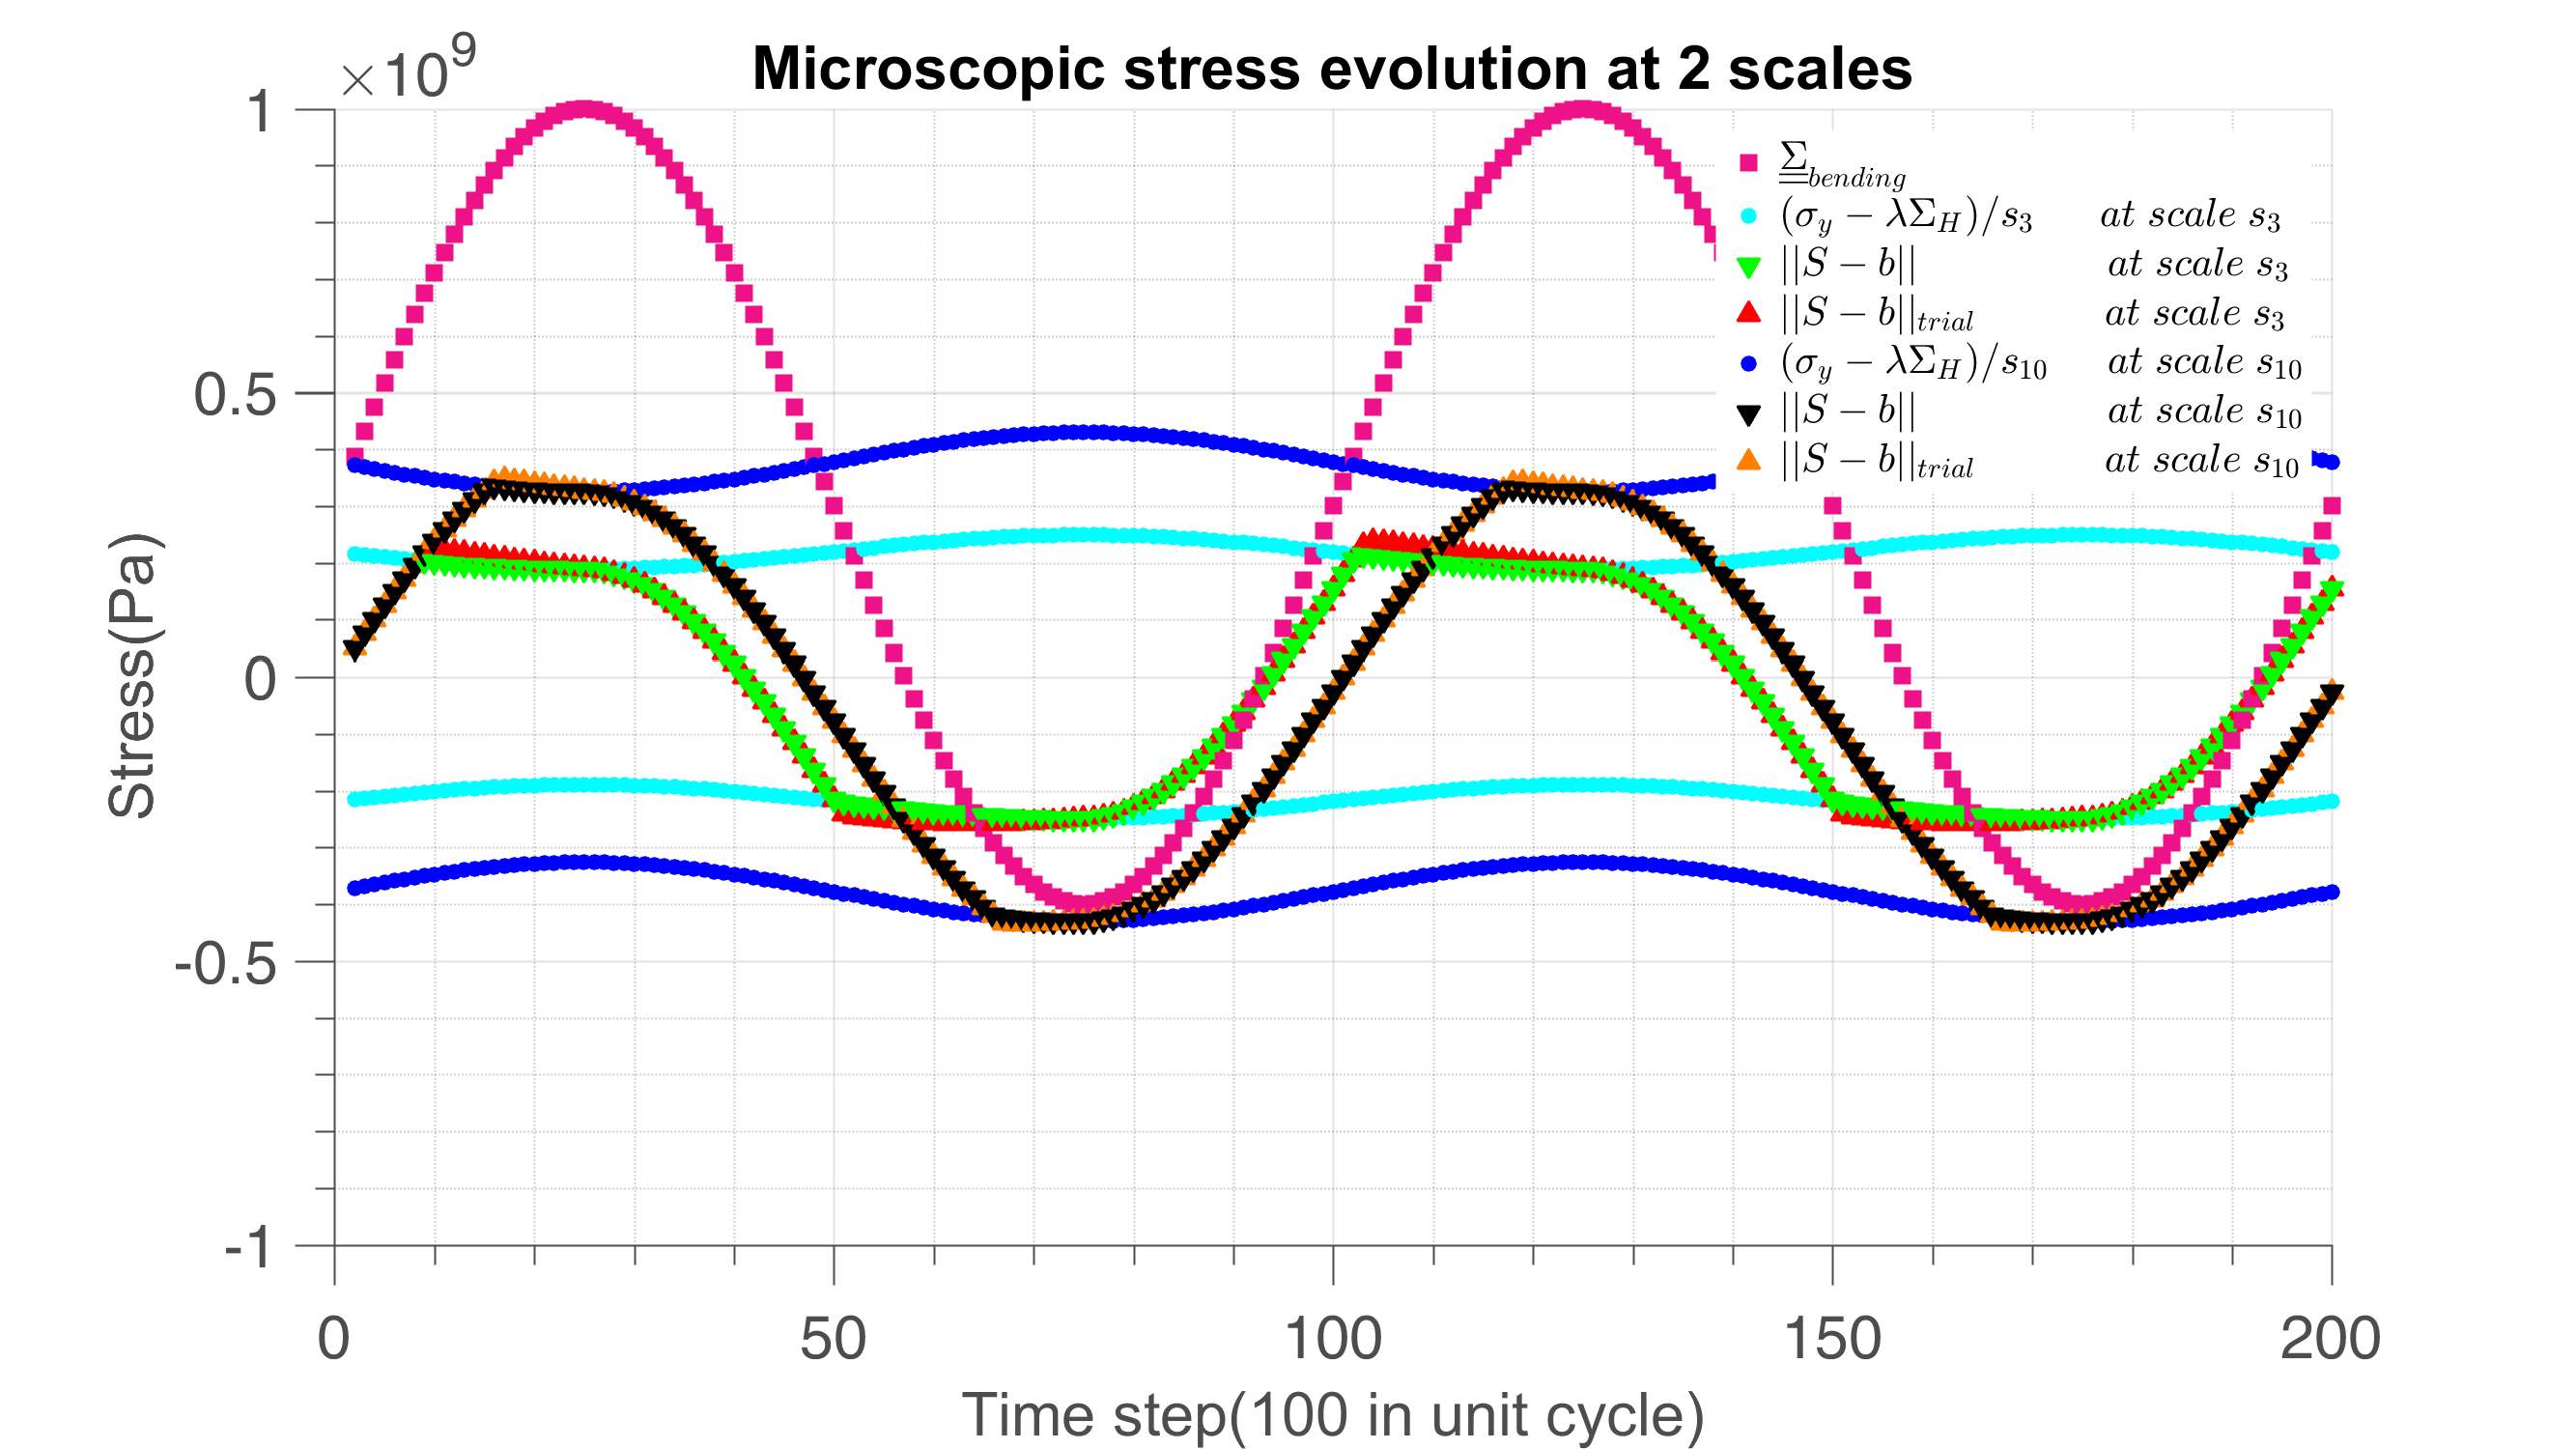
\includegraphics[width=\textwidth]{figures//trialsin_m.png} 
	\caption{Microscopic $\left(  \uline{\uline{S}}-\uline{\uline{b}}\right)_{trial}$ and $\left( \uline{\uline{S}}-\uline{\uline{b}}\right)$ evolution with time under different weakening scales($s_{3}=1.21$ and $s_{10}=1.13$) in sinusoidal load with mean stress=300 MPa}
	\label{fig.trialsinm}
\end{figure}

The time history of dissipated energy is depicted in \figref{fig.W3methods}. We scale $S_{a}$ in the plot to see more clearly the relation between energy dissipation and stress intensity. The choice of $\alpha$ does not affect $W$; it only concerns damage accumulation rate. Smaller $\alpha$ causes faster accumulation.

The ``jump'' in energy evolution is due to activation of new scales while in-between two scales the dissipated energy follows the stress increment at each time step. In other words, because in our method the dissipated energy $W$(\figref{fig.W3methods}), sums energy dissipation at all scales, any additional violation of $\left\|S-b \right\|_{trial}$ at local yield limit(\figref{fig.trialsin0}) introduces an additional dissipation. 

\begin{figure}[!h]
	\centering
	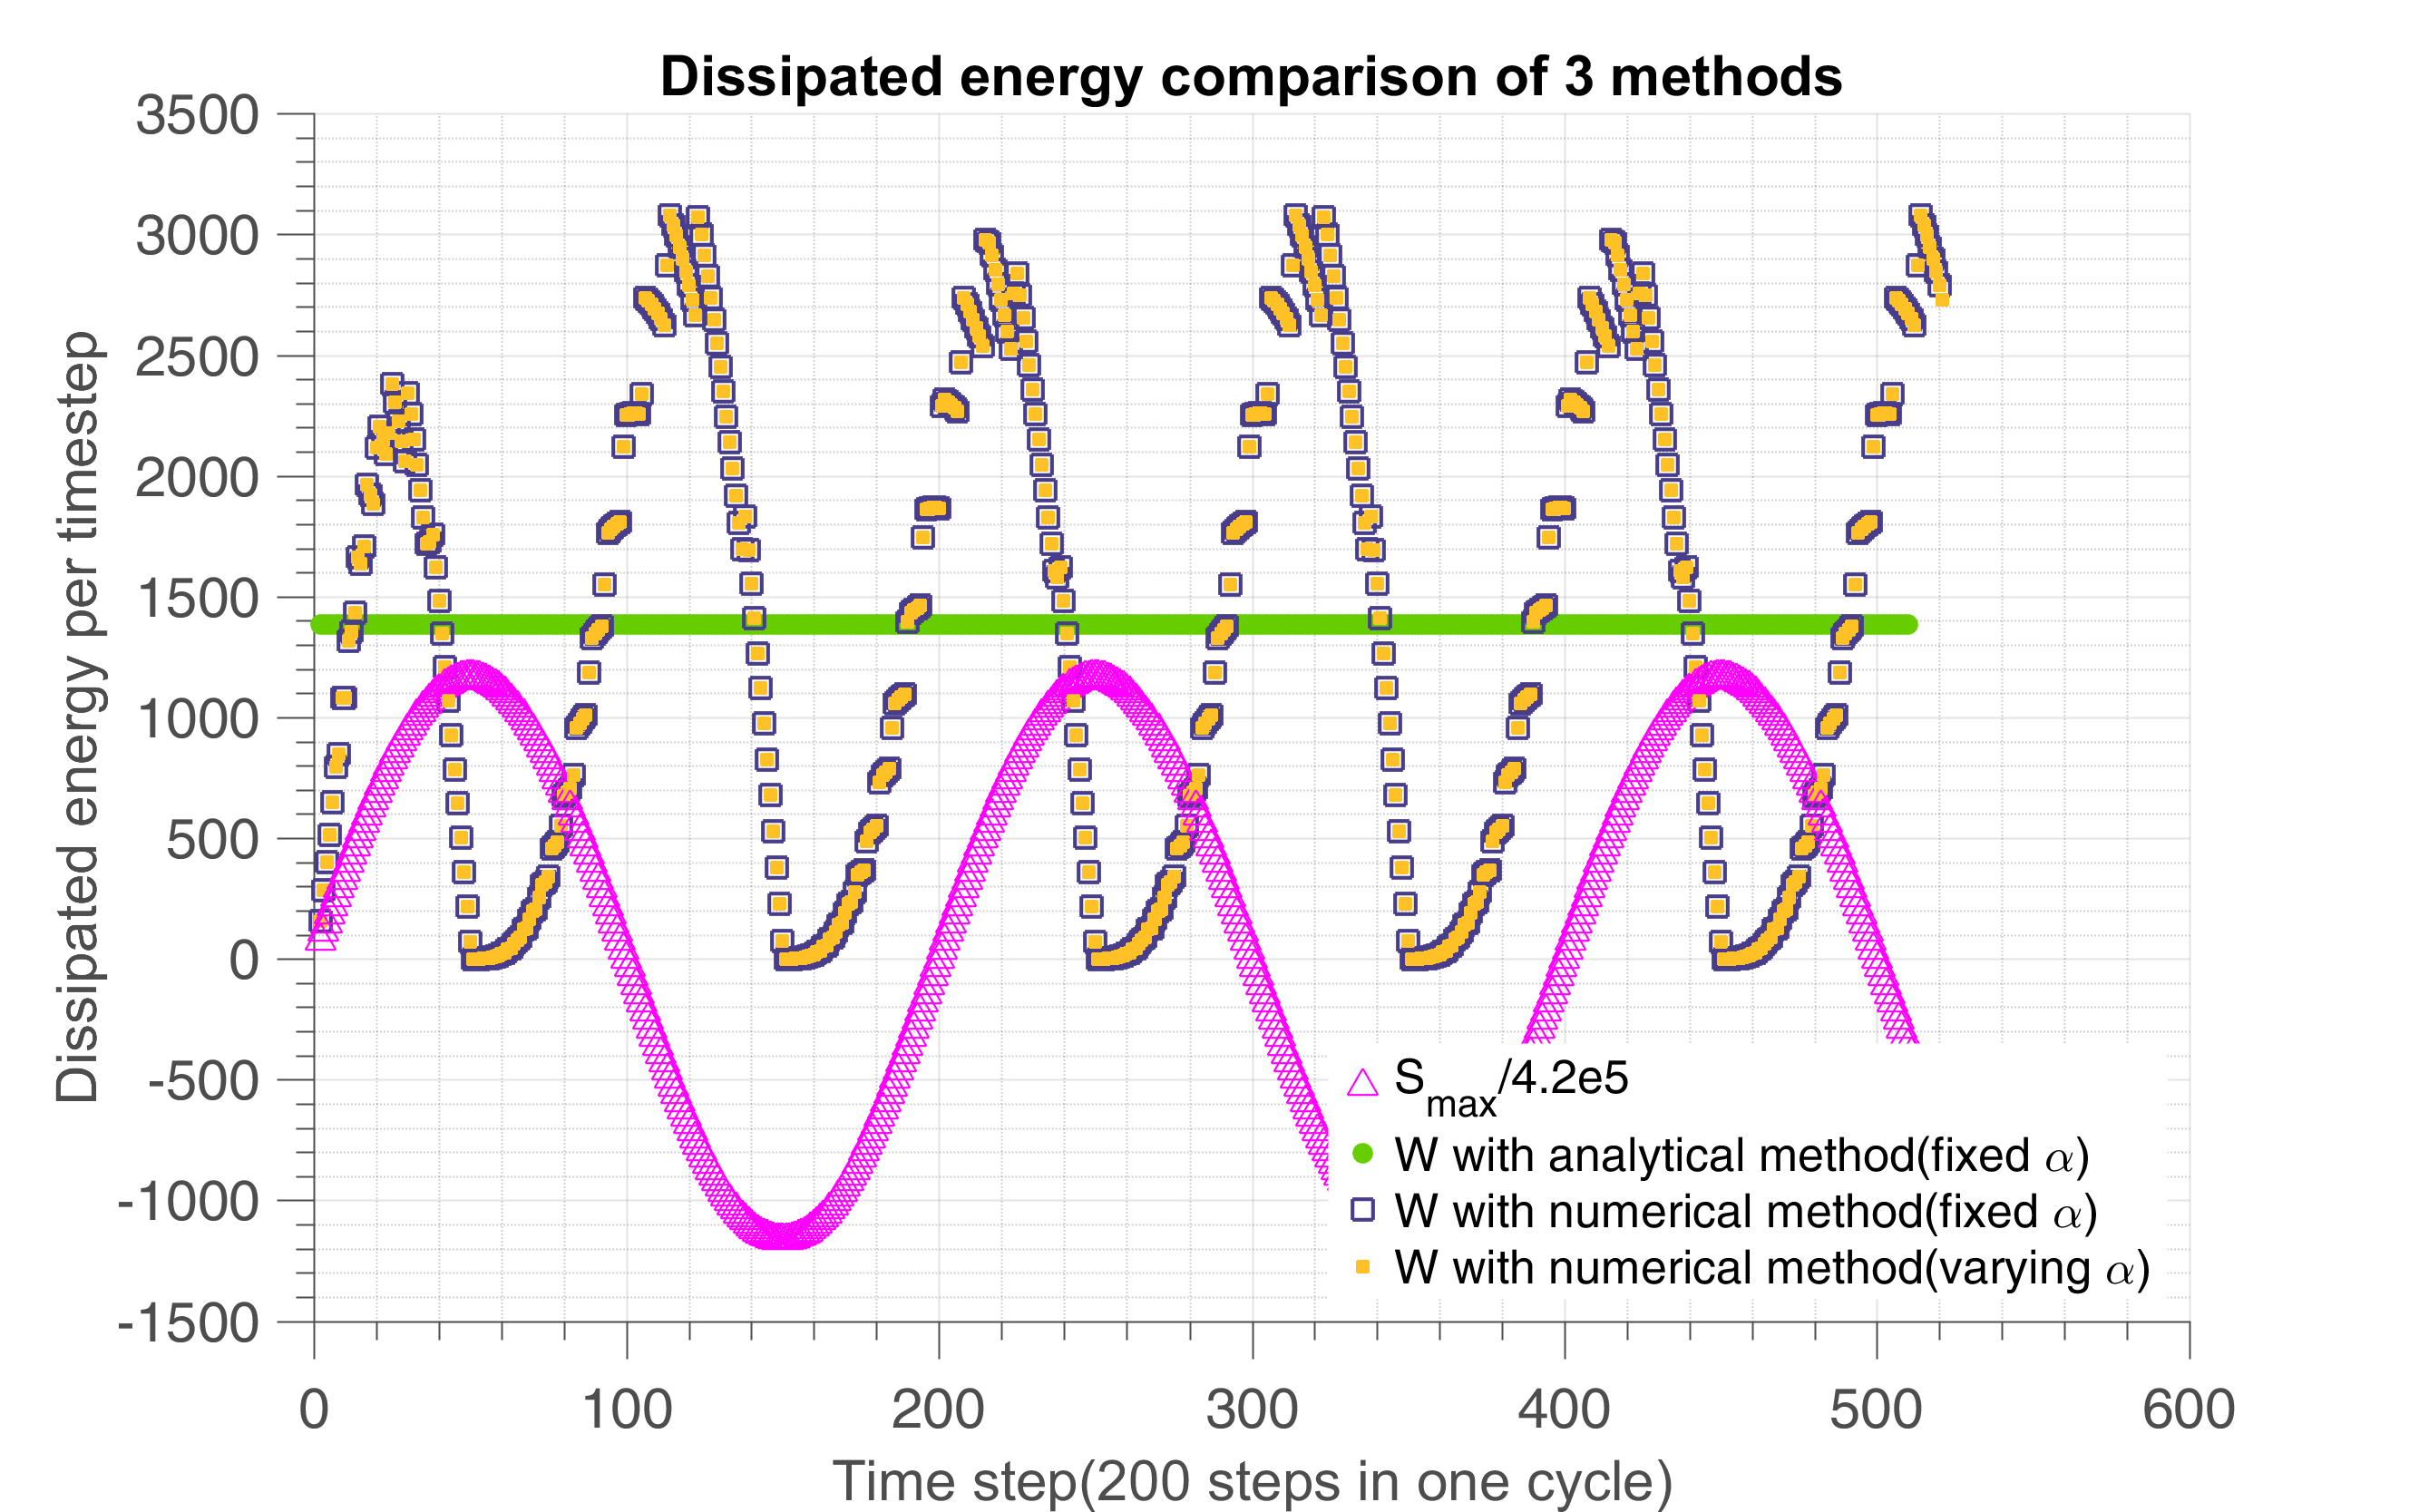
\includegraphics[width=0.95\textwidth]{figures//W_3methods.png} 
	\caption{Validation of dissipated energy in all scales with analytical(method 3) and numerical method(method 1) with $\beta=1.1$,$\Sigma=0.85\sigma_y$. The time evolution of $\alpha$ does not play a role in the dissipation calculation which is normal since $\alpha$ does not enter in the dissipation calculation }
	\label{fig.W3methods}
\end{figure}
\begin{figure}[!h]
	\centering
	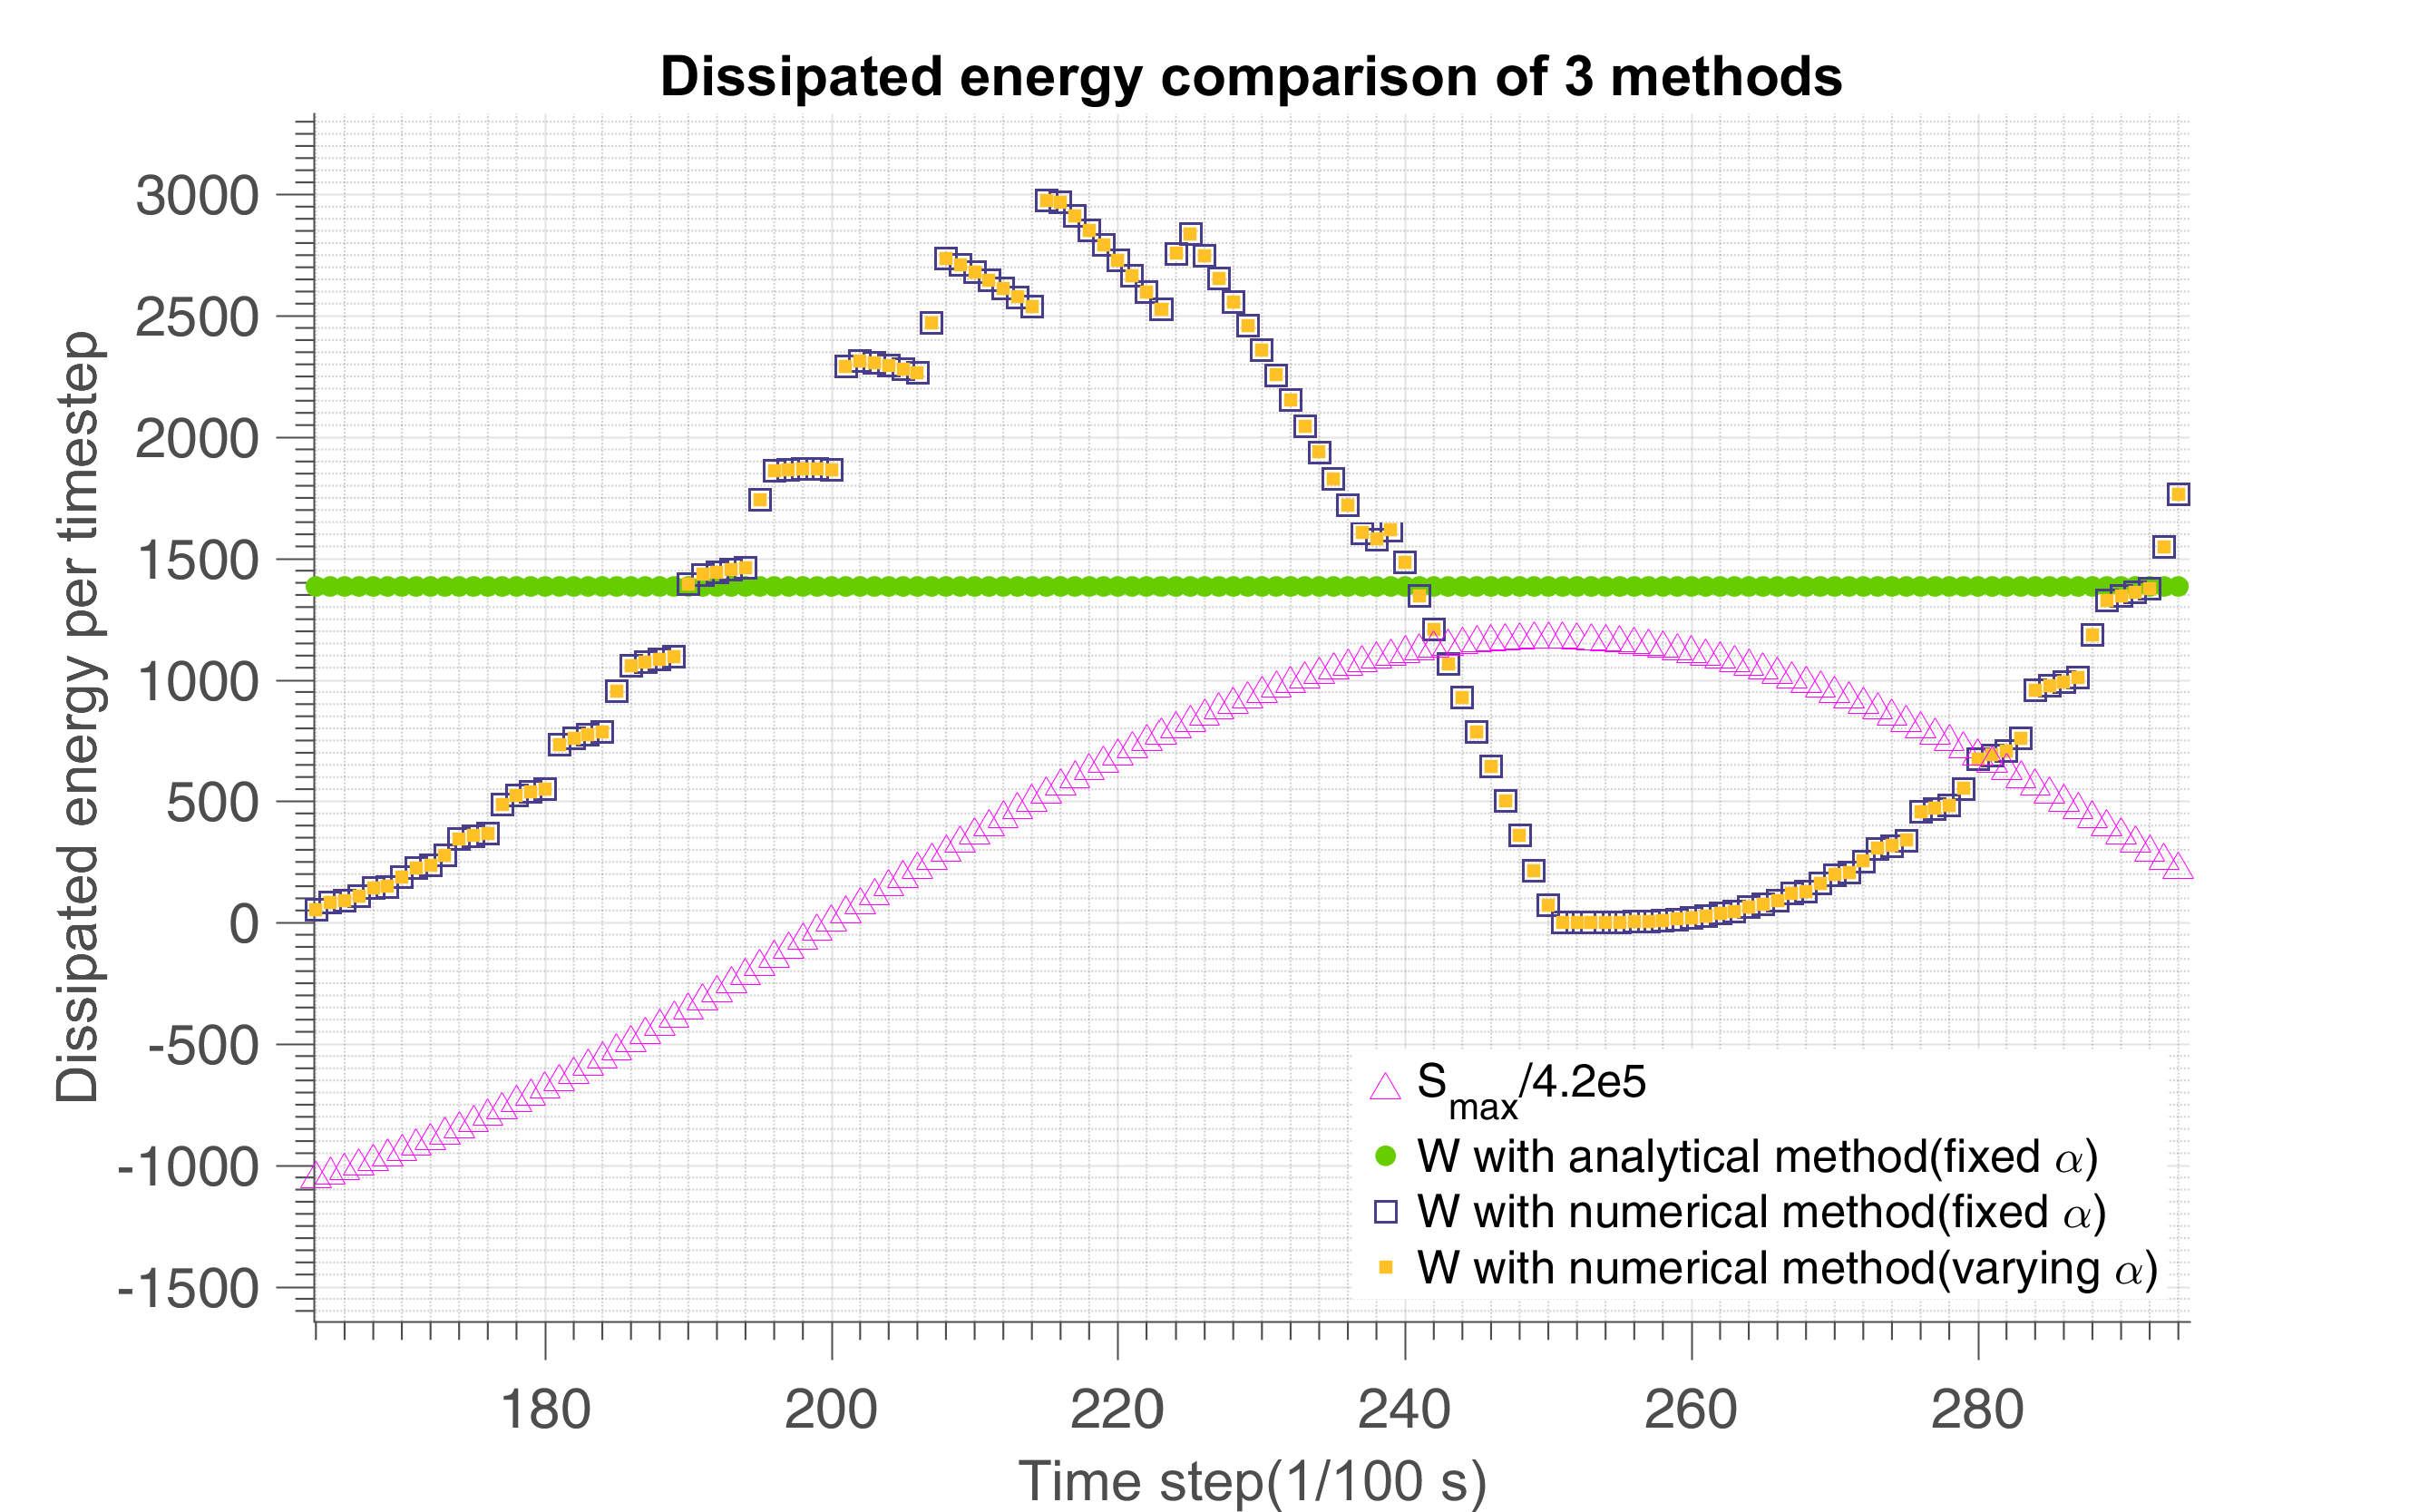
\includegraphics[width=0.95\textwidth]{figures//W_3methods_enlarge.png} 
	\caption{Validation of dissipated energy in all scales with analytical and numerical method(enlargement of \figref{fig.W3methods})}
	\label{fig.W3methodsenlarge}
\end{figure}
\begin{figure}[!h]
	\centering
	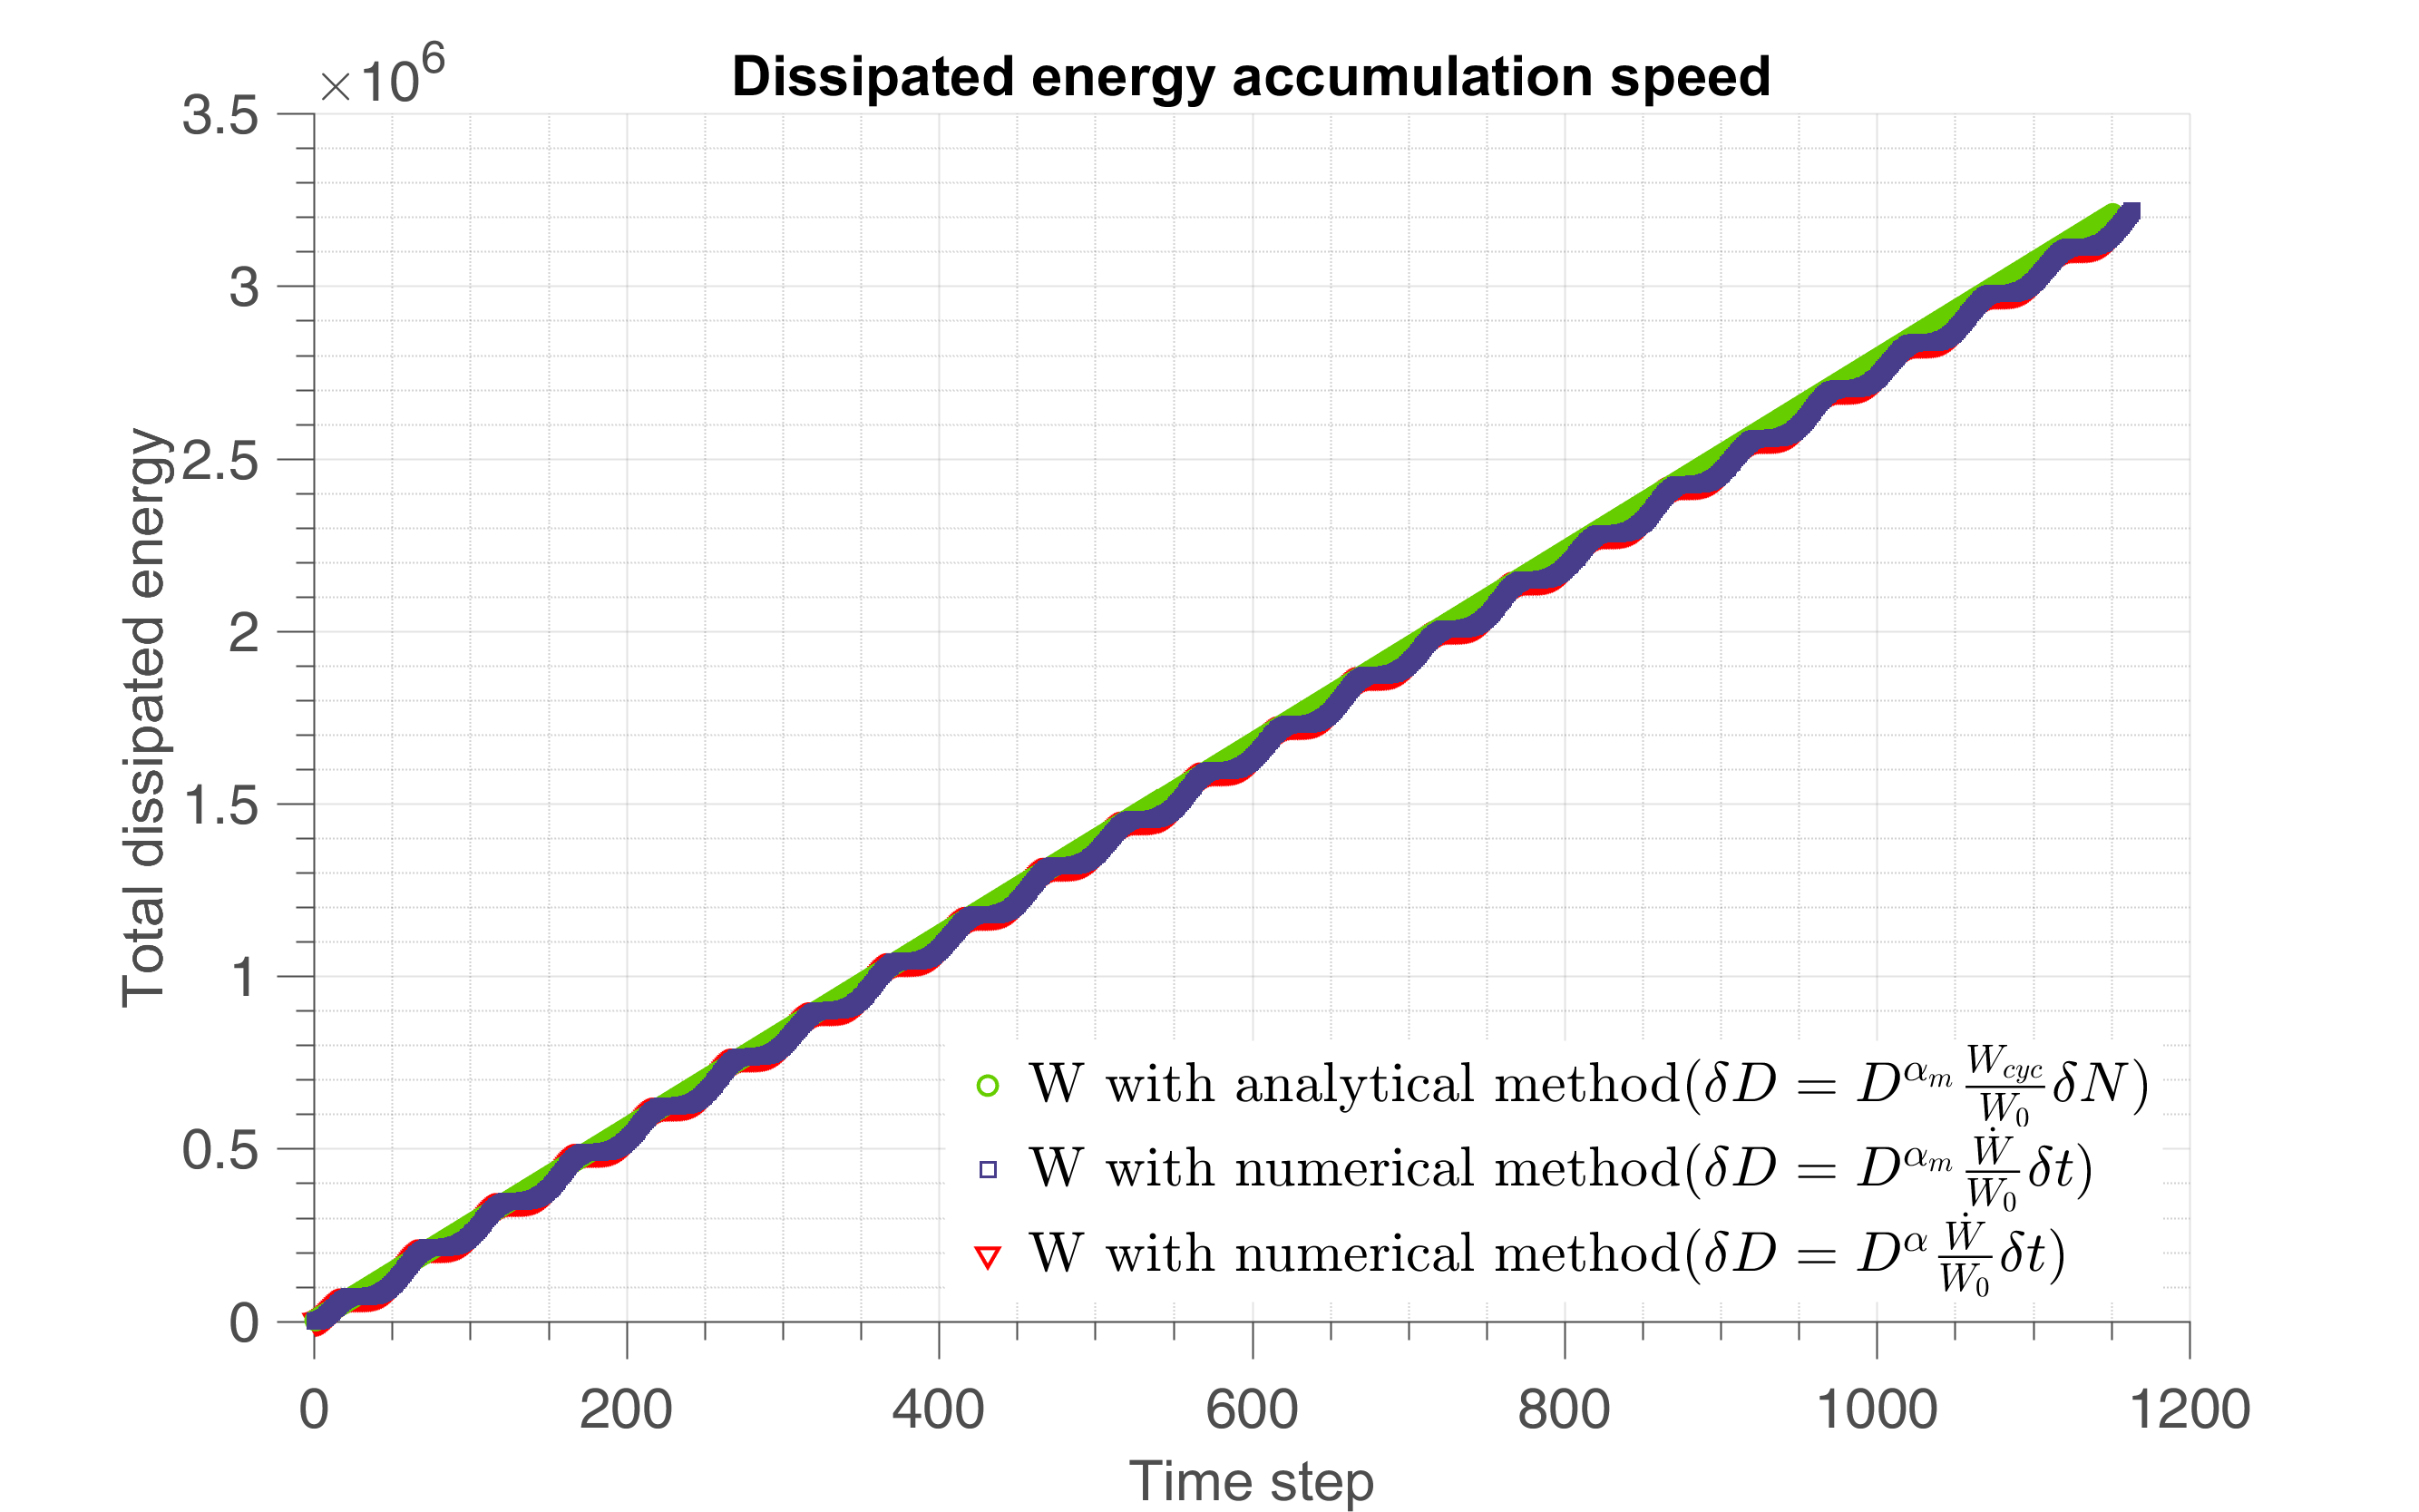
\includegraphics[width=0.95\textwidth]{figures//W_3methods2_100steps.png} 
	\caption{Dissipated energy accumulation through time with different methods, there are 100 time steps in unit cycle}
	\label{fig.W3methods100}
\end{figure}
\begin{figure}[!h]
	\centering
	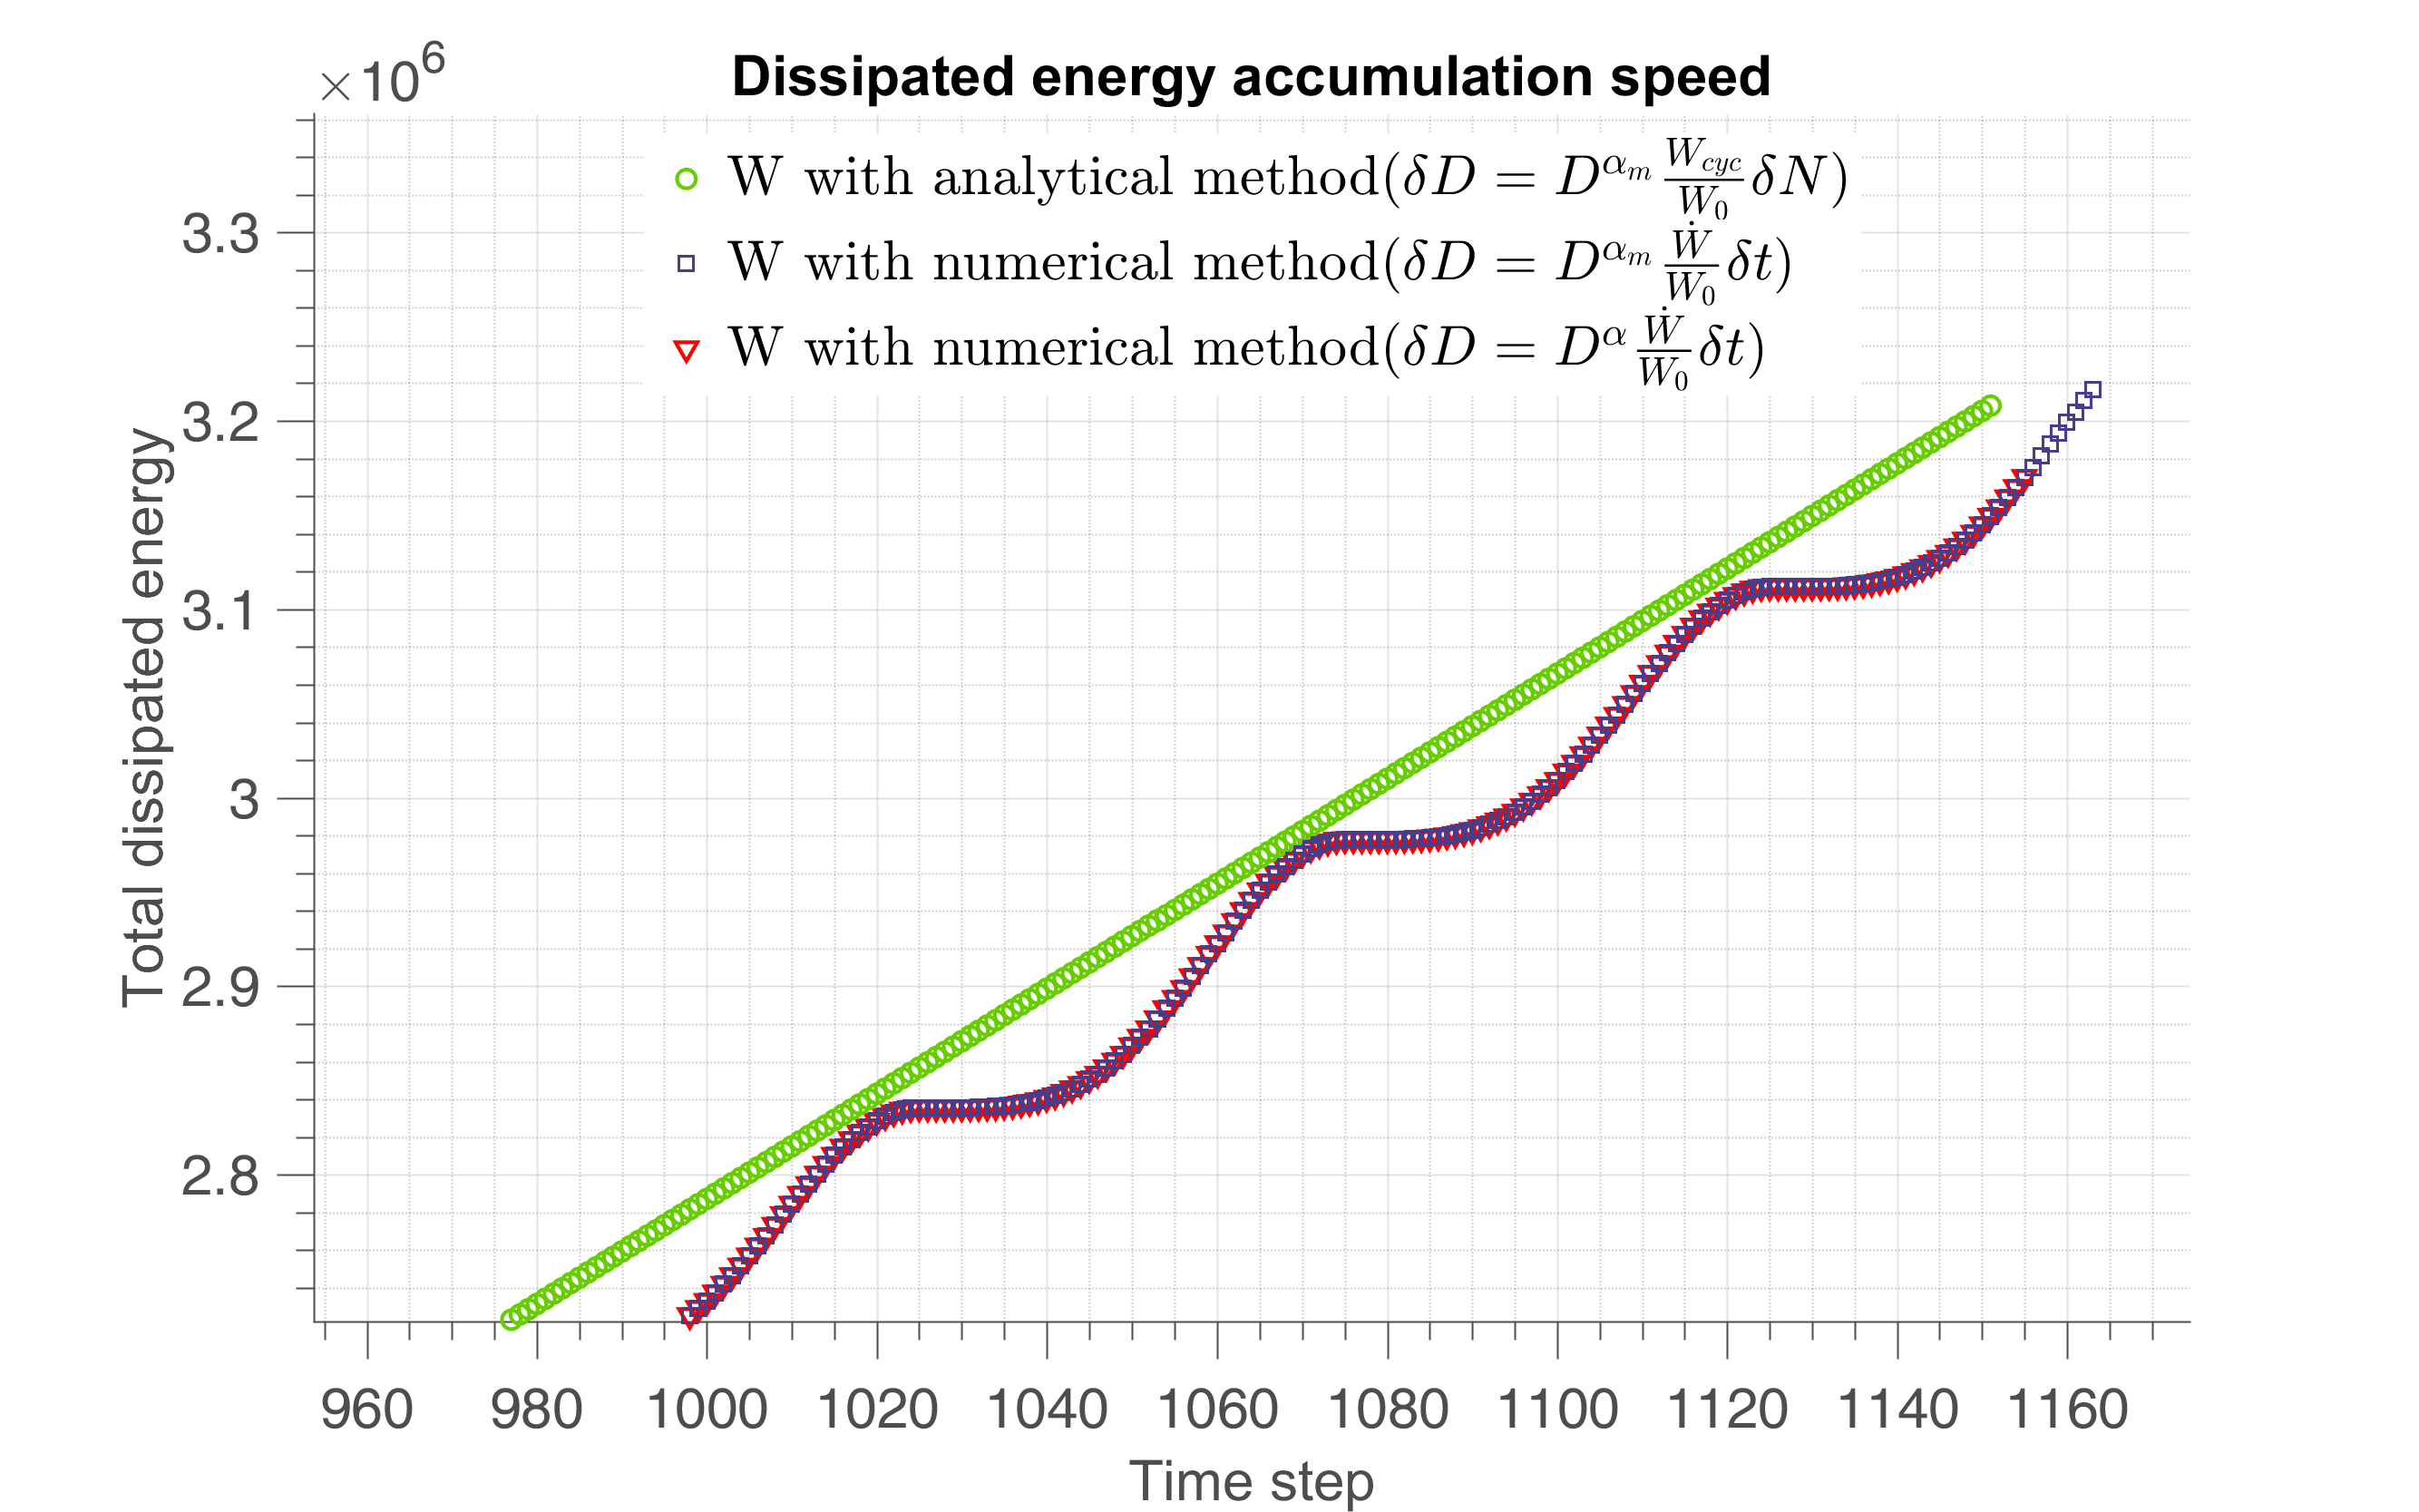
\includegraphics[width=0.95\textwidth]{figures//W_3methods_100steps_enlarge.png} 
	\caption{Dissipated energy accumulation through time with of 3 methods(enlargement of \figref{fig.W3methods100})}
	\label{fig.W3methods2enlarge}
\end{figure}
\begin{figure}[!h]
	\centering
	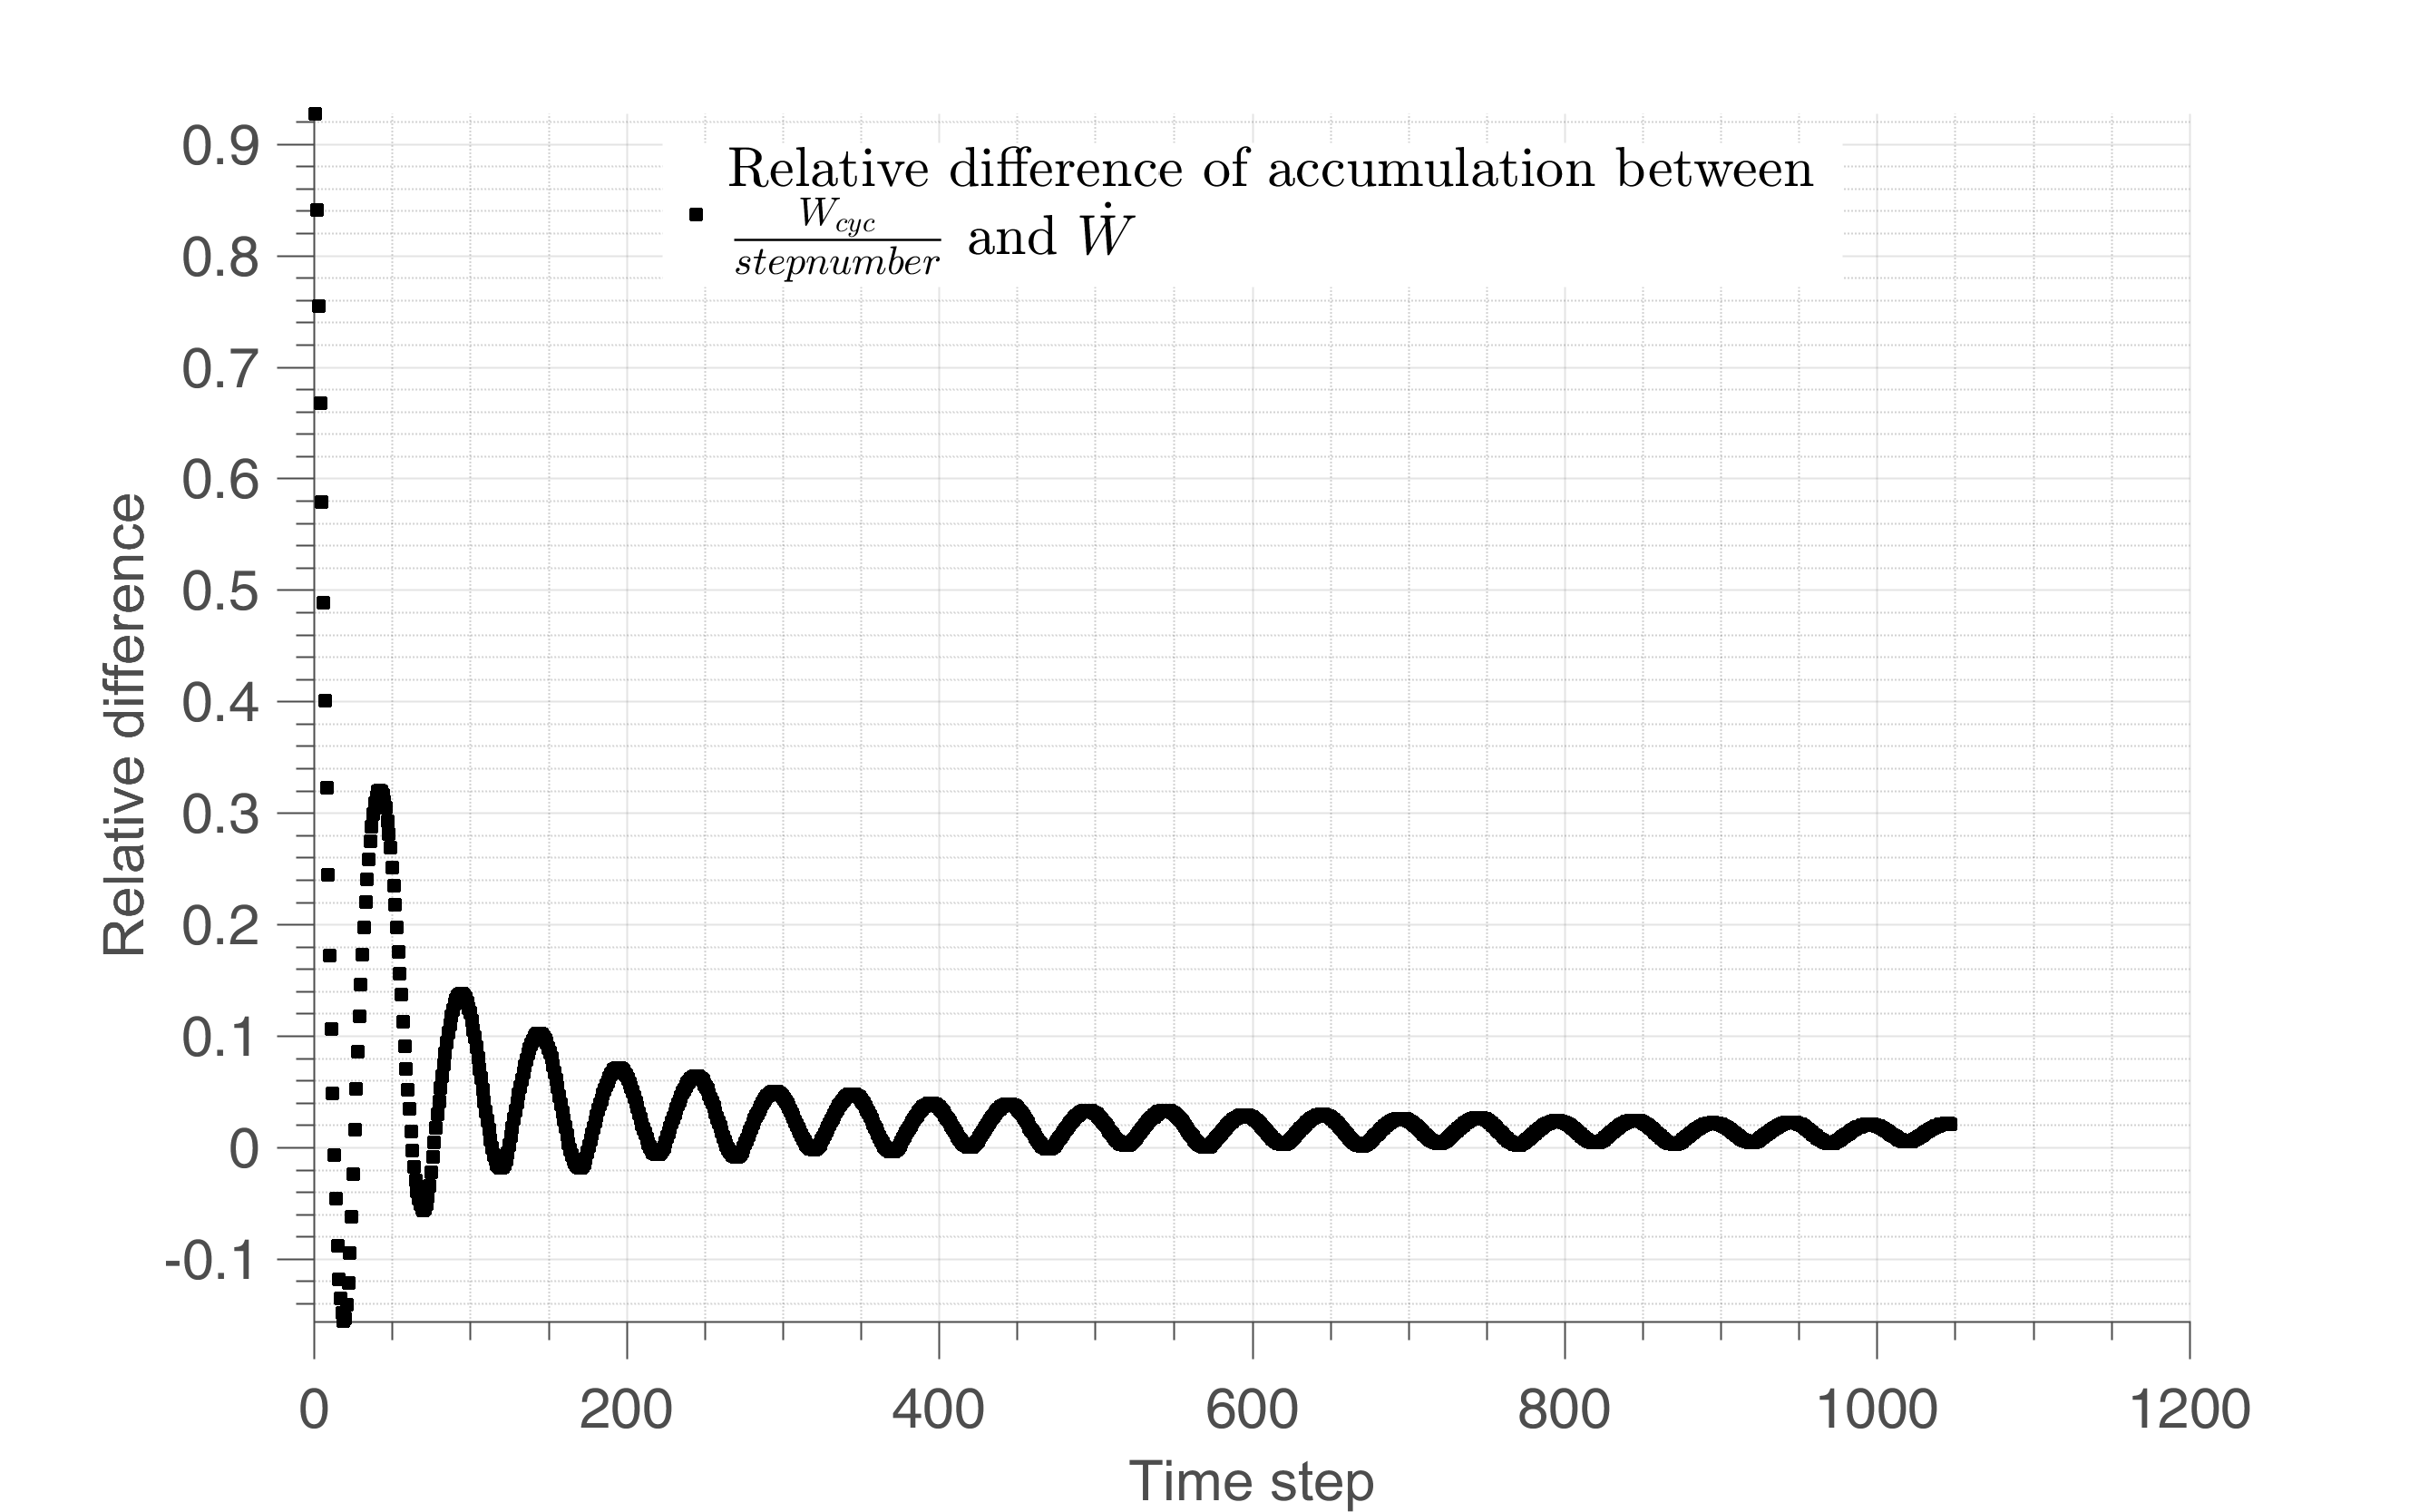
\includegraphics[width=0.95\textwidth]{figures//W_3methods_diff_100steps.png} 
	\caption{Relative difference $\dfrac{W_{analytical}-W_{numerical}}{W_{analytical}}$ between analytical energy loss and numerical one with $\alpha$ varying with time of \figref{fig.W3methods100}}
	\label{fig.W3methodsdiff}
\end{figure}
\begin{figure}[!h]
	\centering
	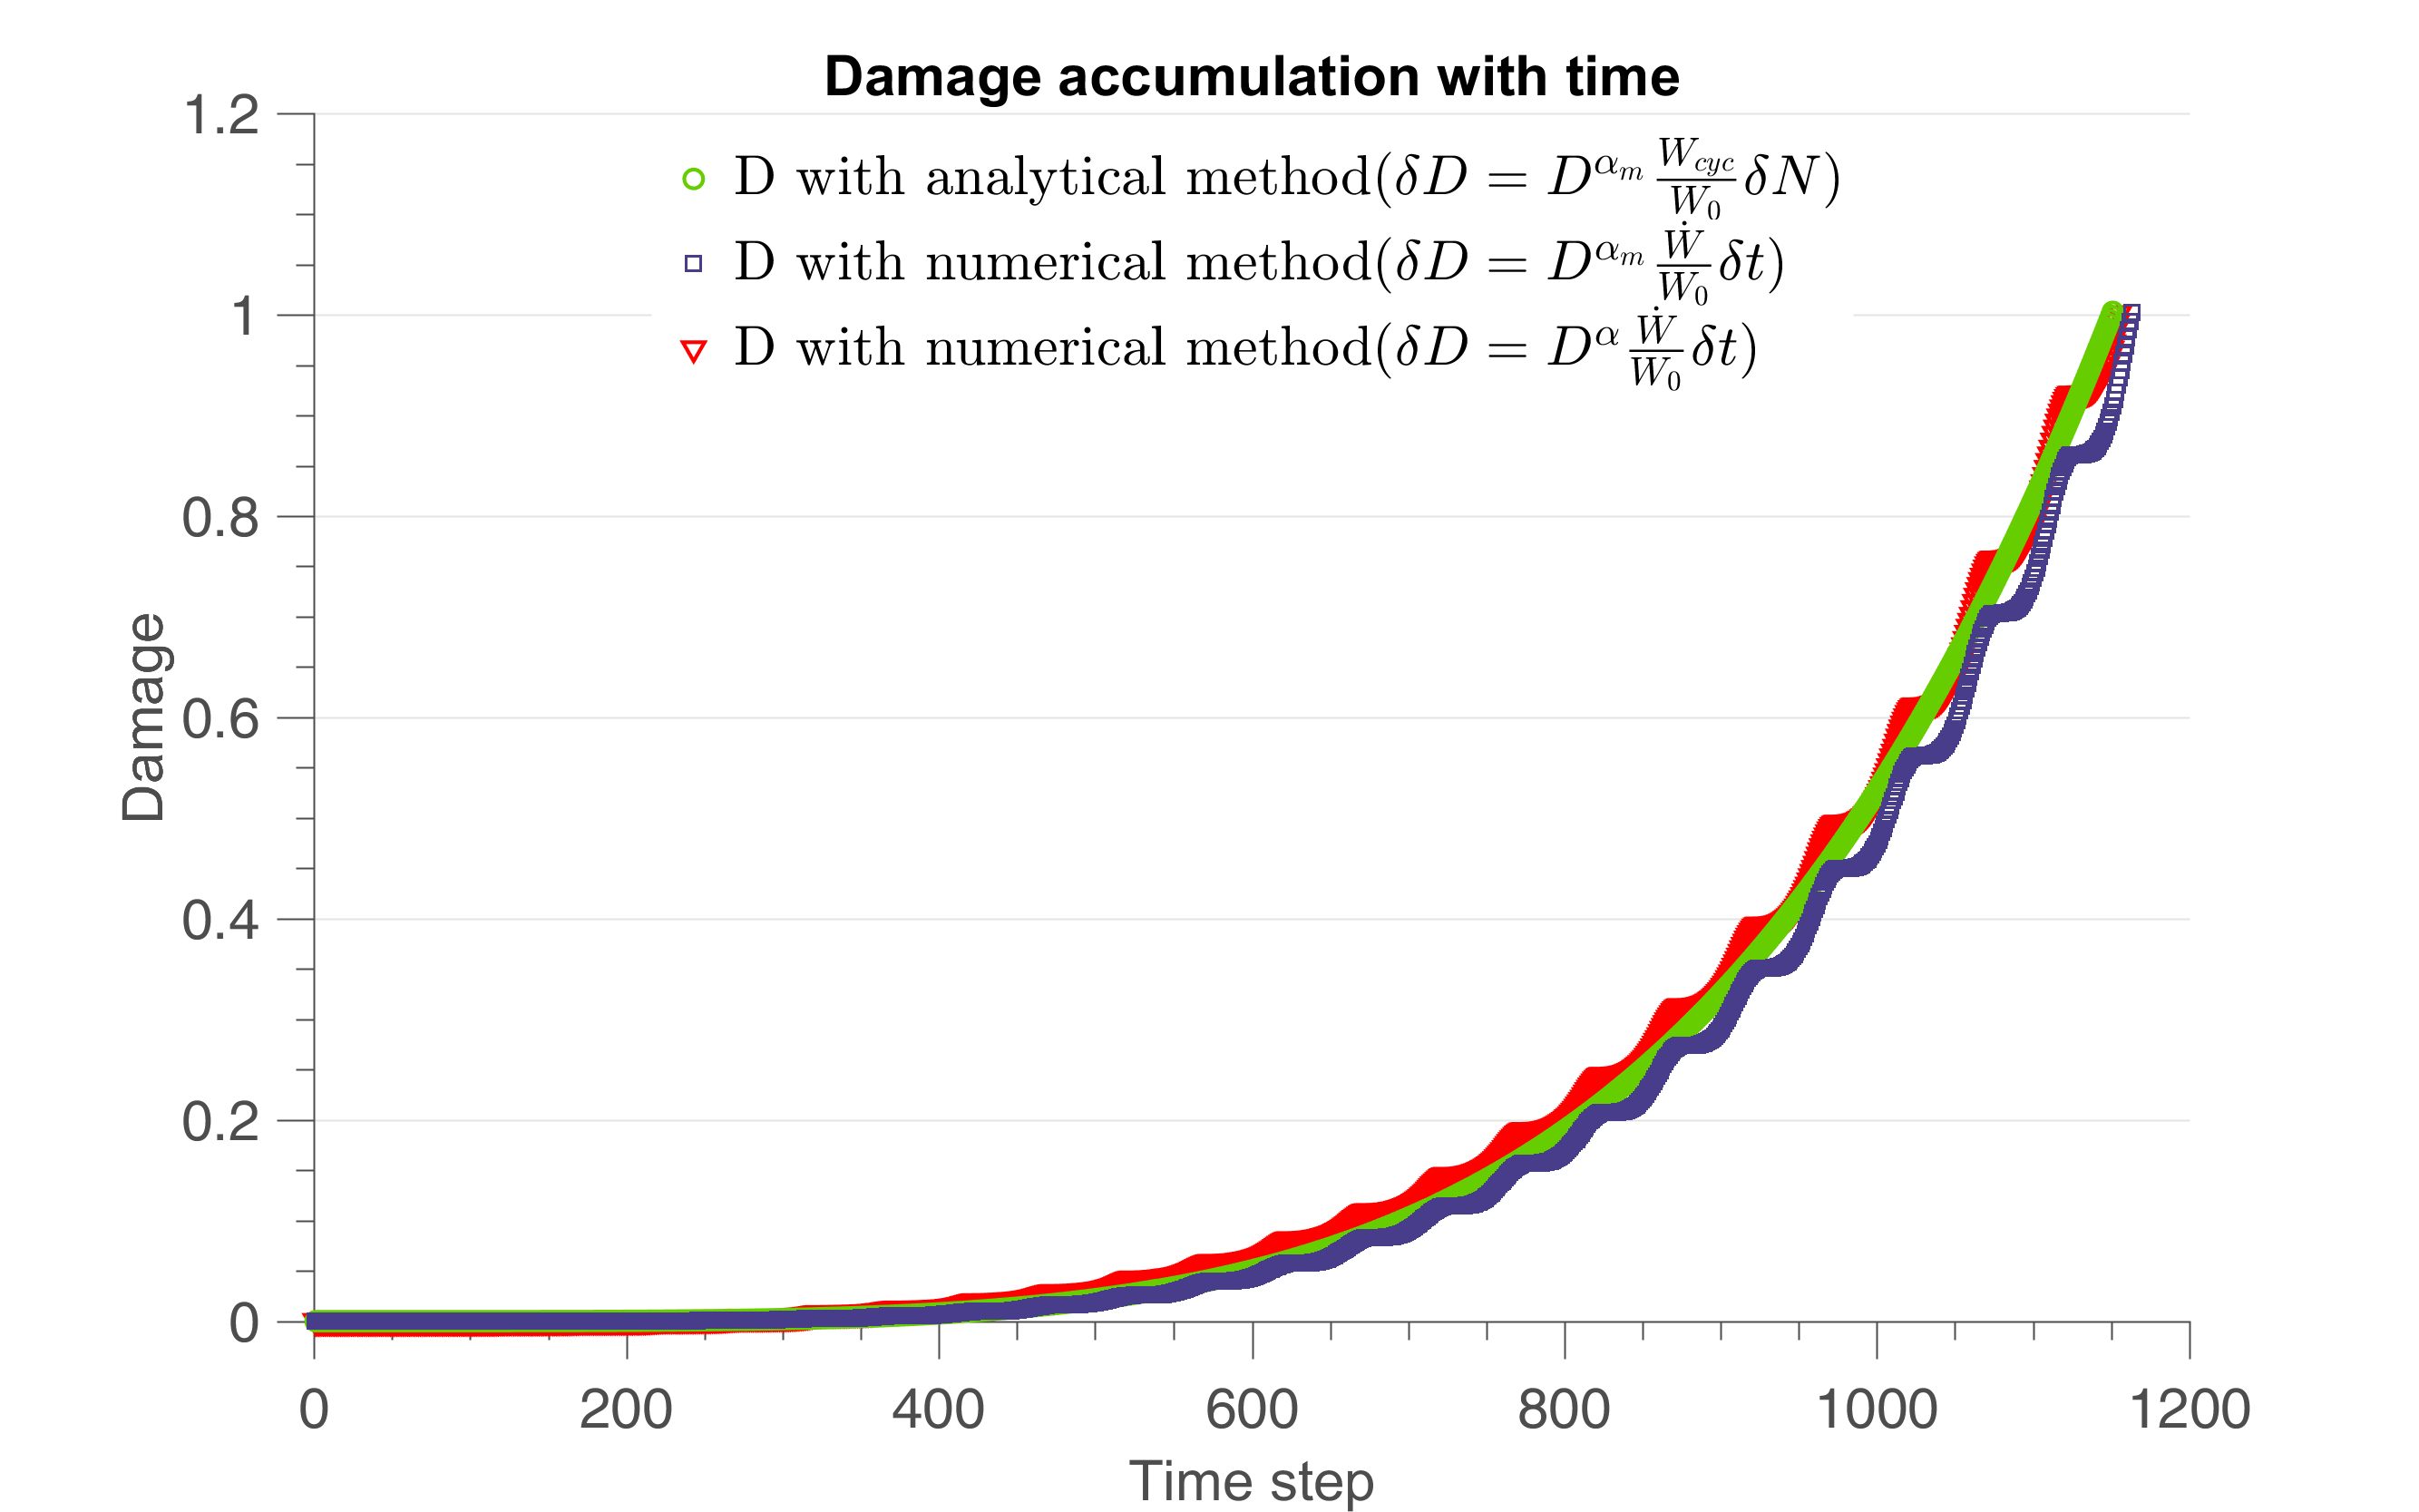
\includegraphics[width=\textwidth]{figures//D_3methods2_100steps.png} 
	\caption{Damage evolution with time under sinusoidal load with different methods, there are 100 time steps in unit cycle($\beta=1.1$,$\Sigma=0.85\sigma_y$)}
	\label{fig.damsin100}
\end{figure}

\begin{figure}[!h]
	\centering
	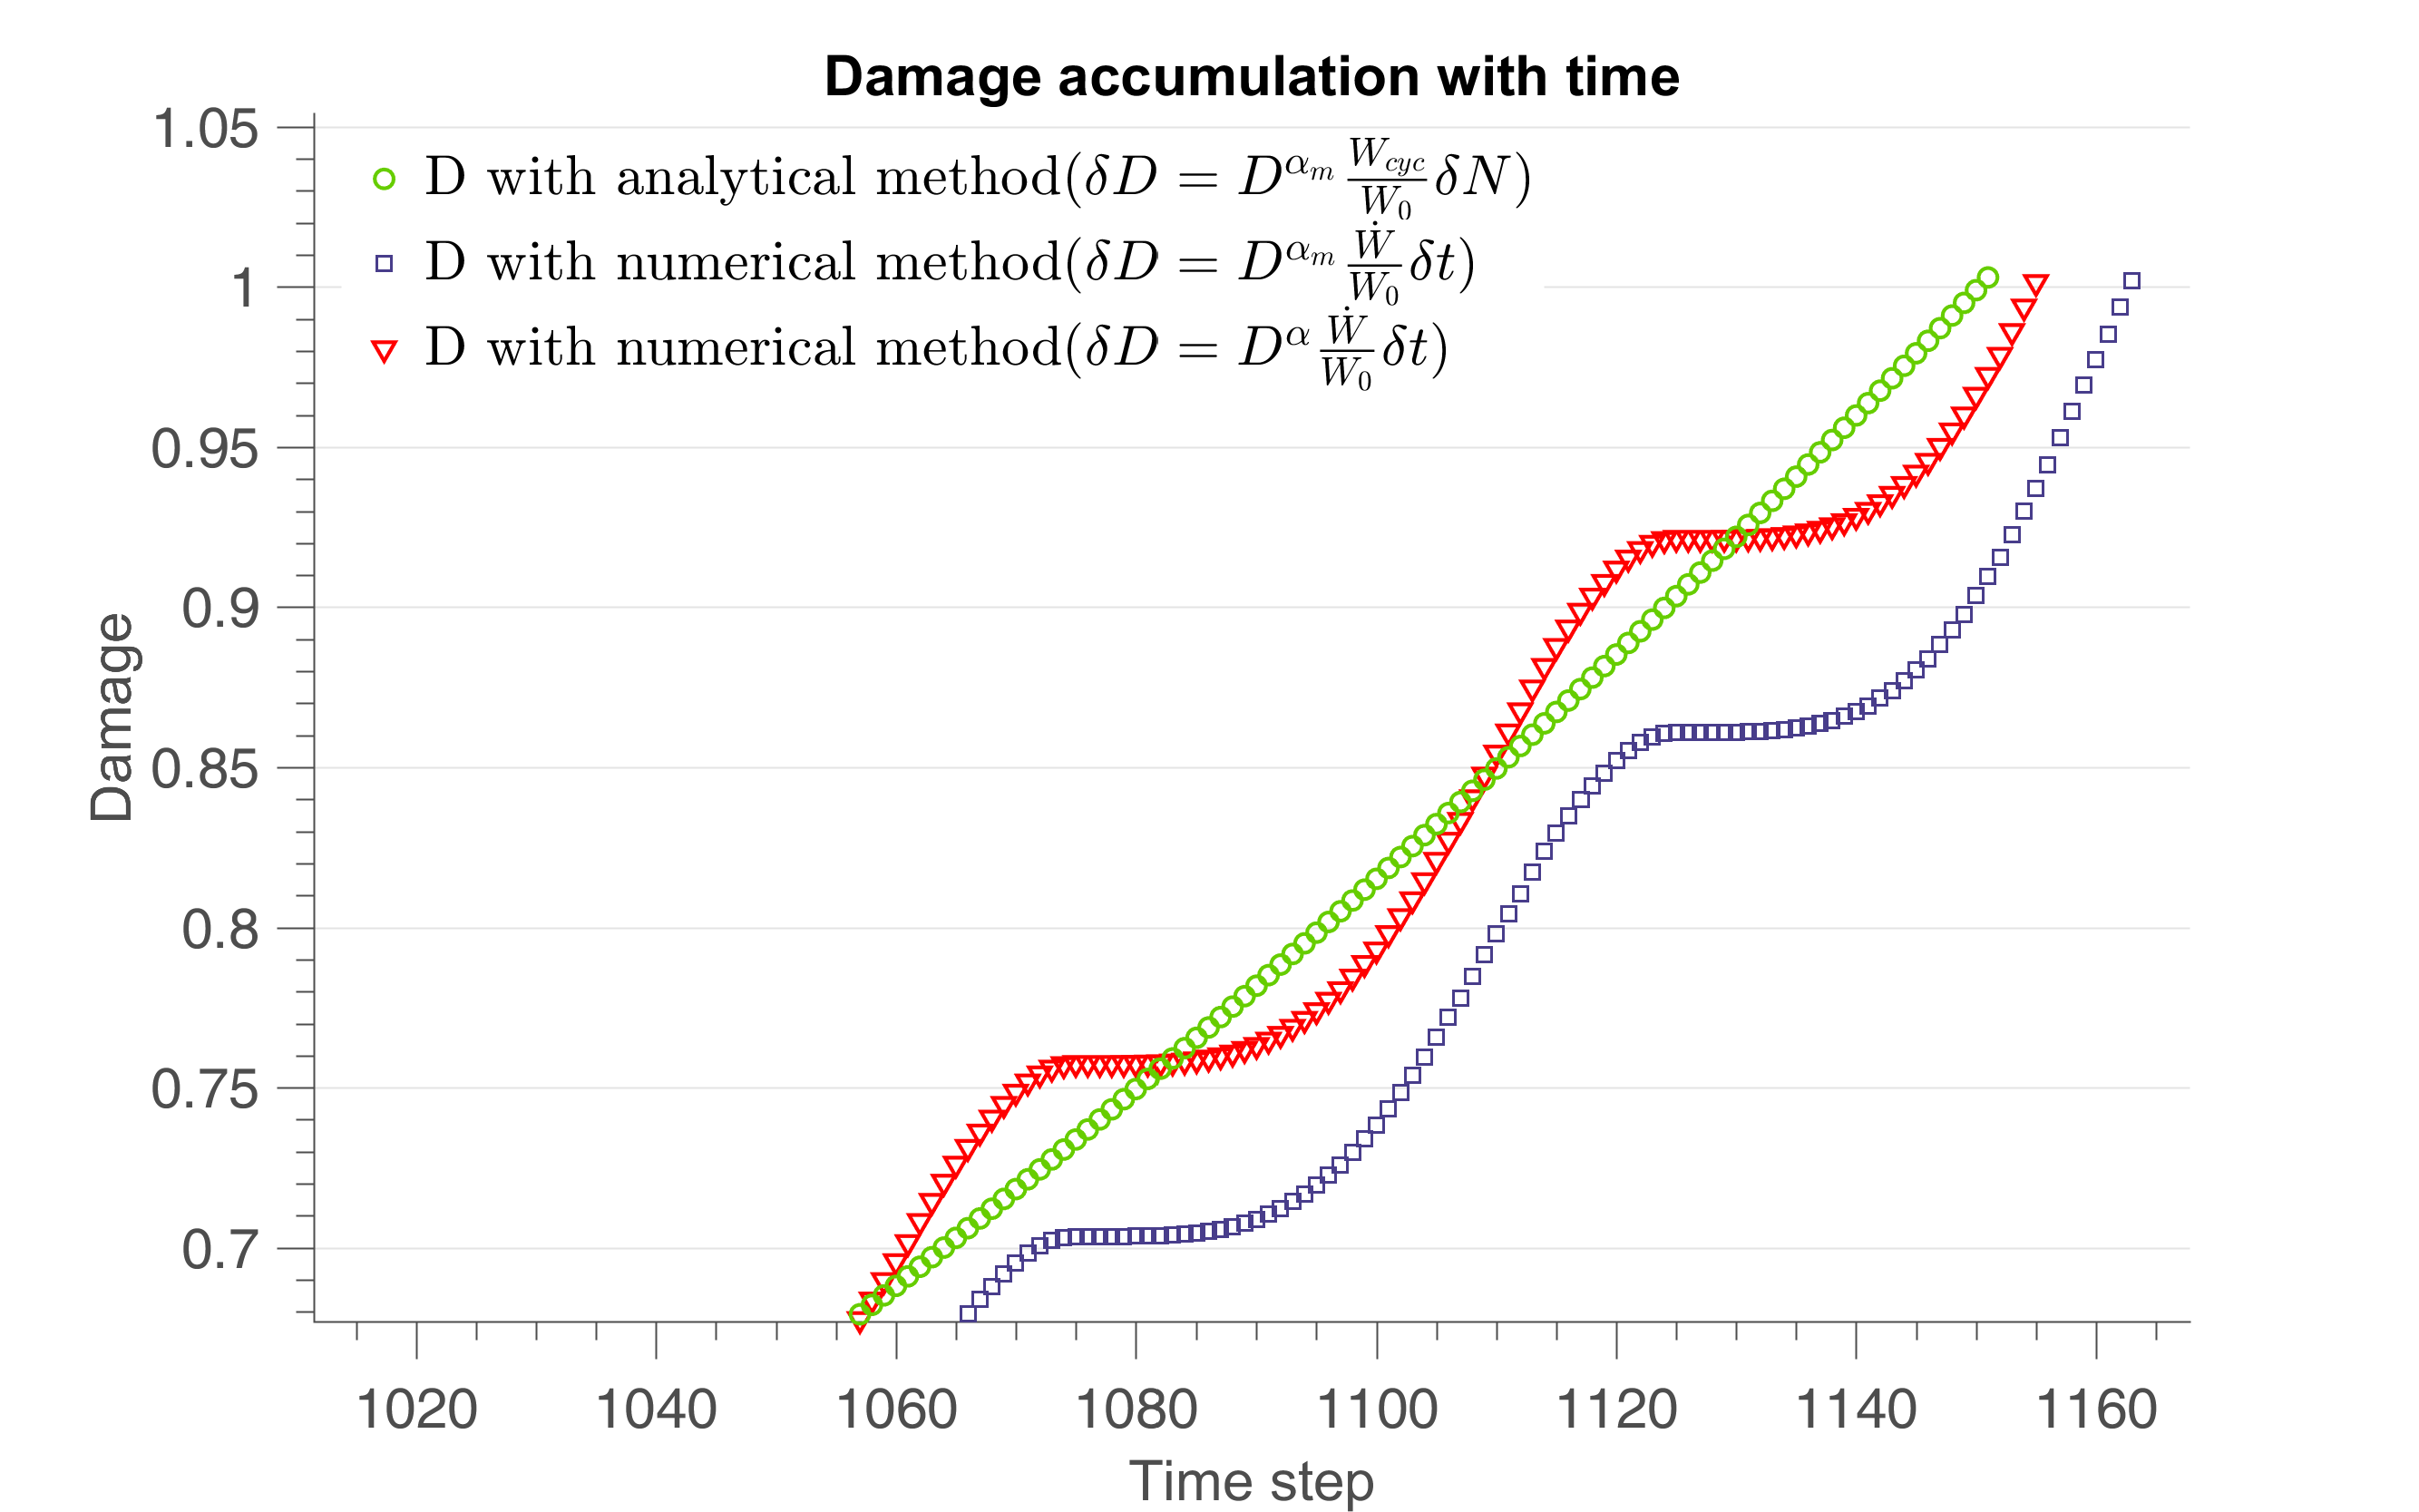
\includegraphics[width=\textwidth]{figures//D_3methods_100steps_enlarge.png} 
	\caption{Damage evolution with time under sinusoidal load with two different methods(enlargement of \figref{fig.damsin100})}
	\label{damsinenglarge}
\end{figure}

\begin{figure}[!h]
	\centering
	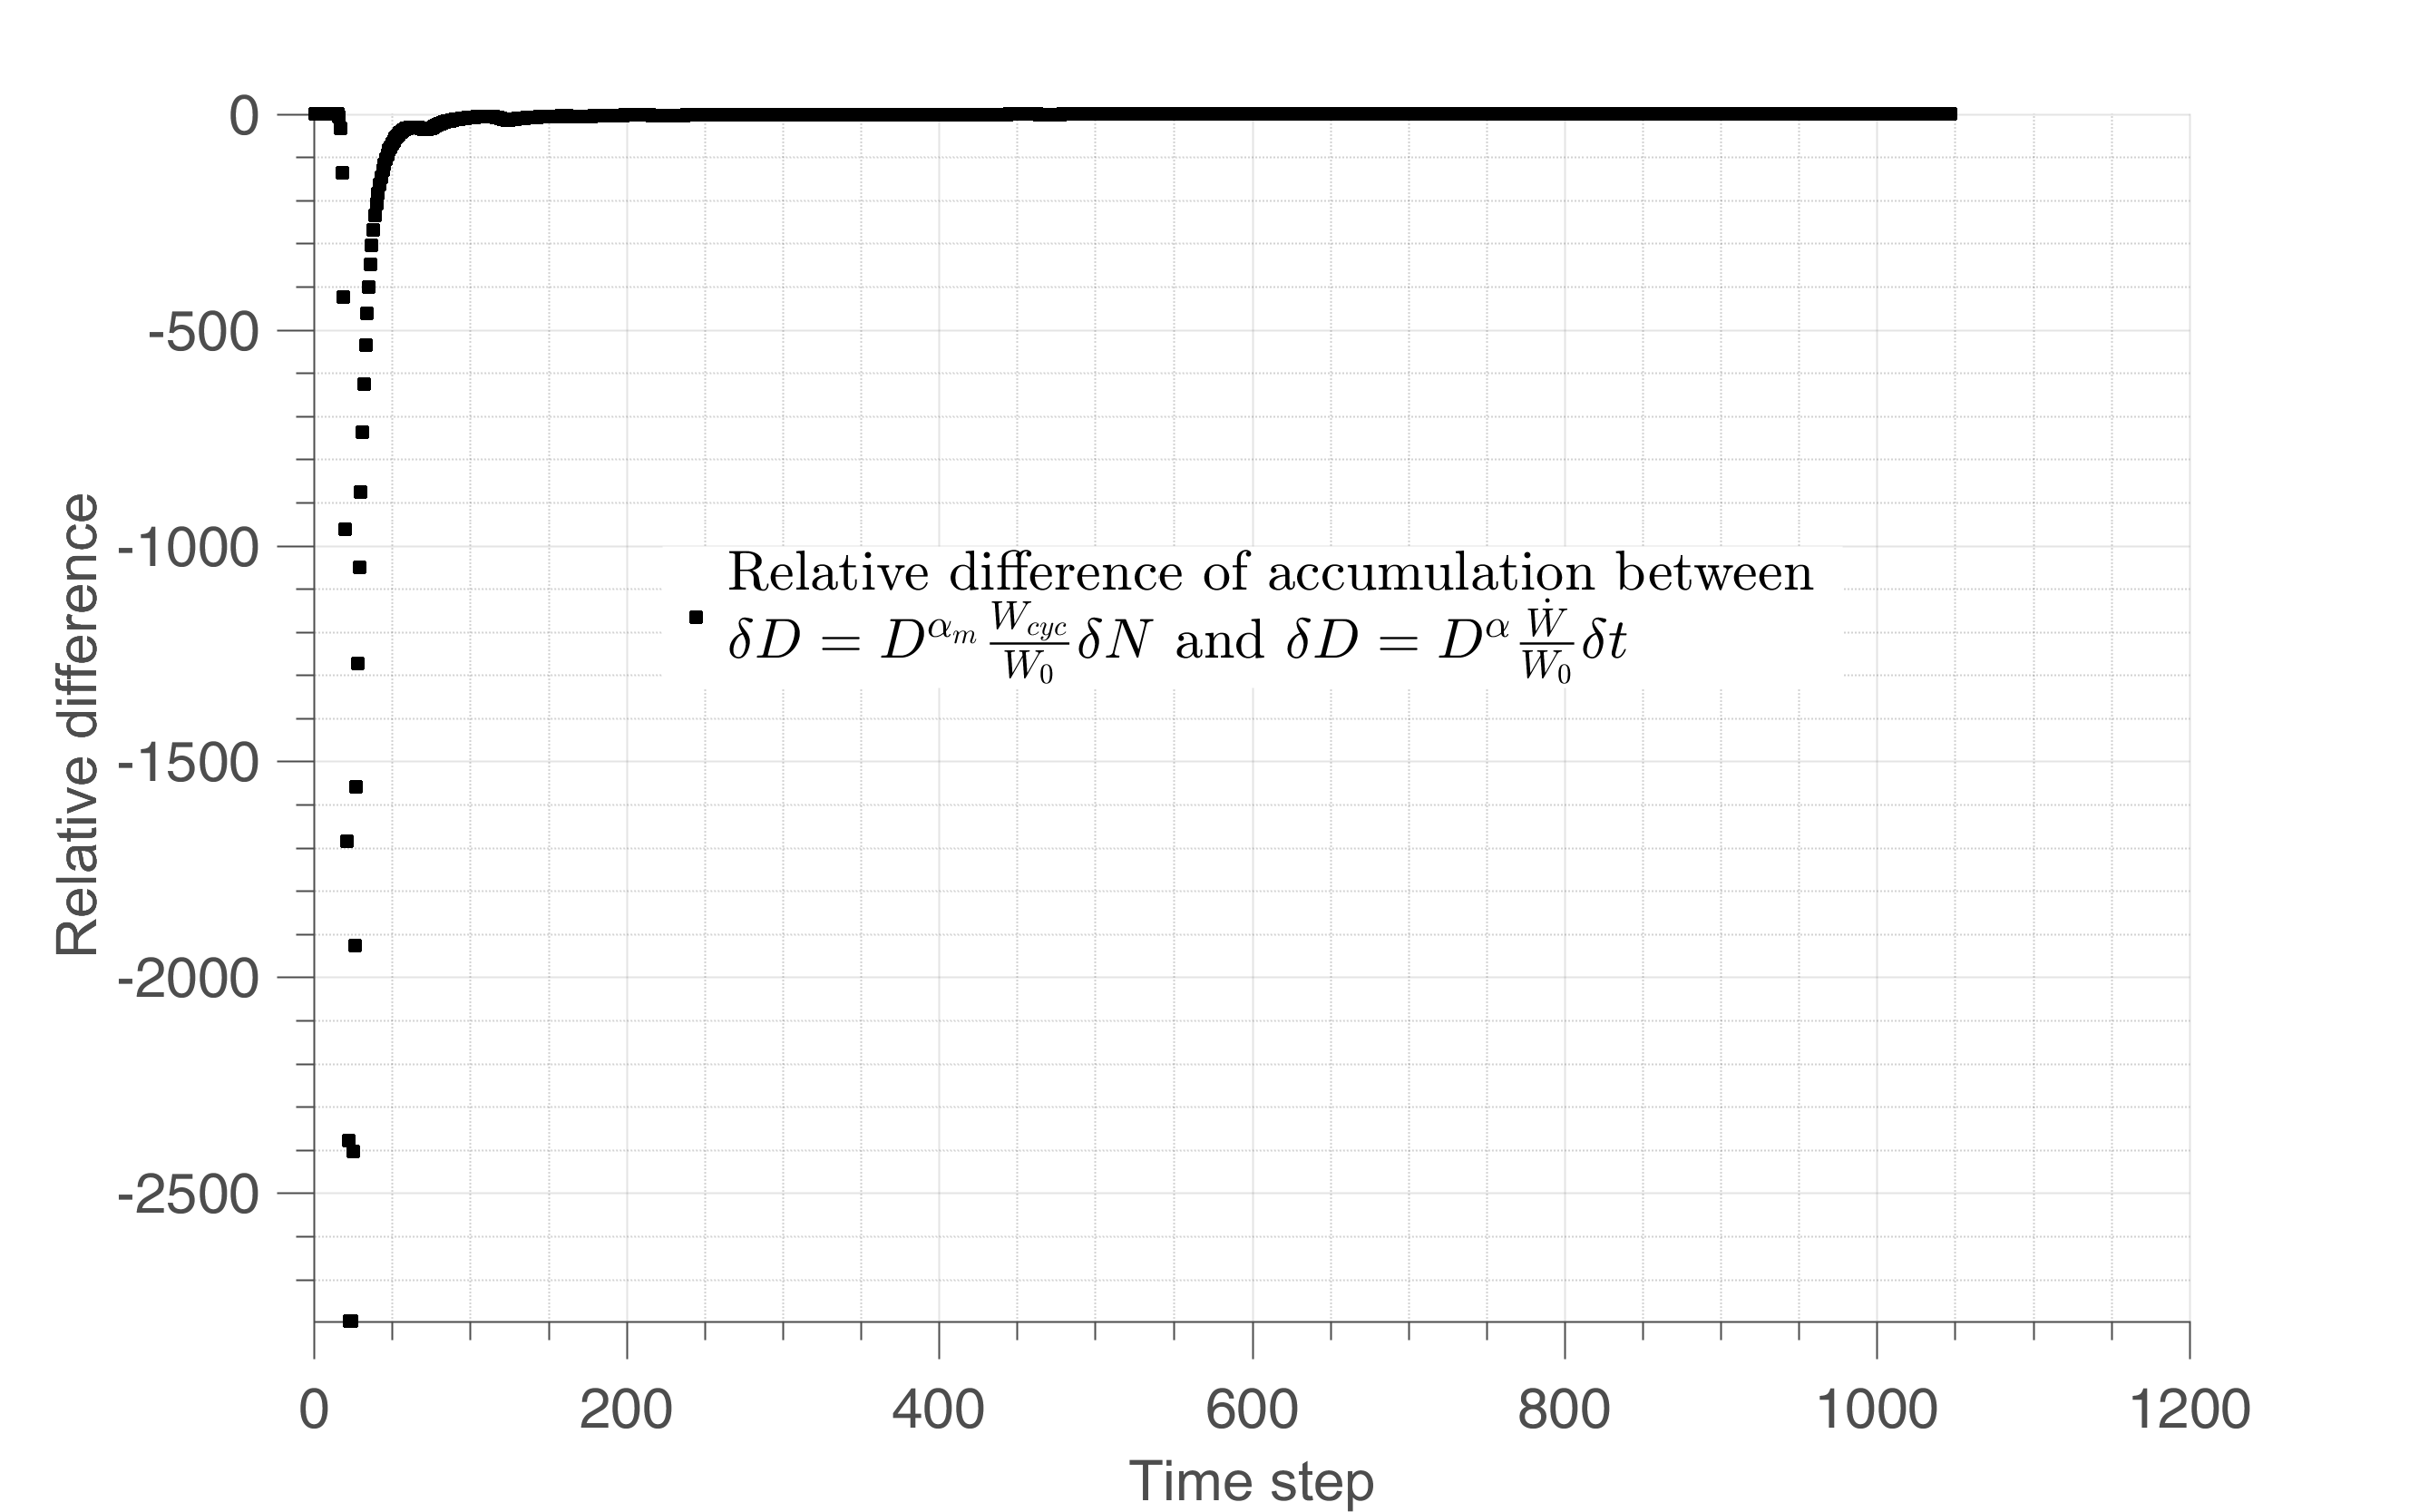
\includegraphics[width=\textwidth]{figures//D_3methods_diff_100steps.png} 
	\caption{Relative difference $\dfrac{D_{analytical}-D_{numerical}}{D_{analytical}}$ evolution with time of \figref{fig.damsin100}}
	\label{Damagediff}
\end{figure}
We take the mean value of $\alpha$ during all the iteration process of numerical method as $\alpha_{m}$. The energy and damage accumulation is shown in \figref{fig.W3methods100} and \figref{fig.damsin100}. Here we give 100 time steps in one cycle to see the relative difference between changing $\alpha$ and $\alpha_{m}$, also $\dot{W}$ and $W_{cyc}/stepnumber$  method. The more time steps we give, the more precision we get. The relative difference between analytical energy loss and numerical one is shown in \figref{fig.W3methodsdiff} from which we conclude that the three methods converge in terms of elastic energy dissipation, but due to nonlinear effects the damage evolution does not have the same history per cycle. The frozen $\alpha$ delays damage, the varying $\alpha$ increases damage during the phase of strong loading. The difference has a significant impact if damage occurs with very few cycles. It will not when computing on a large number of cycles.

The cyclic load calculation is only valid for very simple such as proportional loading in fatigue. However, the convergence of the two methods is based on the small value of $\beta$(close to 1), in case of large values of $\beta$(typically around 5), the numerical strategy gives shorter life than the analytical one due to extreme non-linearity in the energy dissipation history per cycle. The relative error is around 20\% as shown in \figref{fig.W3methods_bigbeta_04y} and \figref{fig.W3methods_bigbeta_08y}. Nevertheless the analytical formula can still be used as a comparison group to verify the numerical results. And in the identification process we need the analytical form to fit the $S-N$ curve of a certain material. The outcome is satisfactory. Hence, to be more general for any loading history, we adopt the numerical method after identification of $\beta$. 

\begin{figure}[!h]
	\centering
	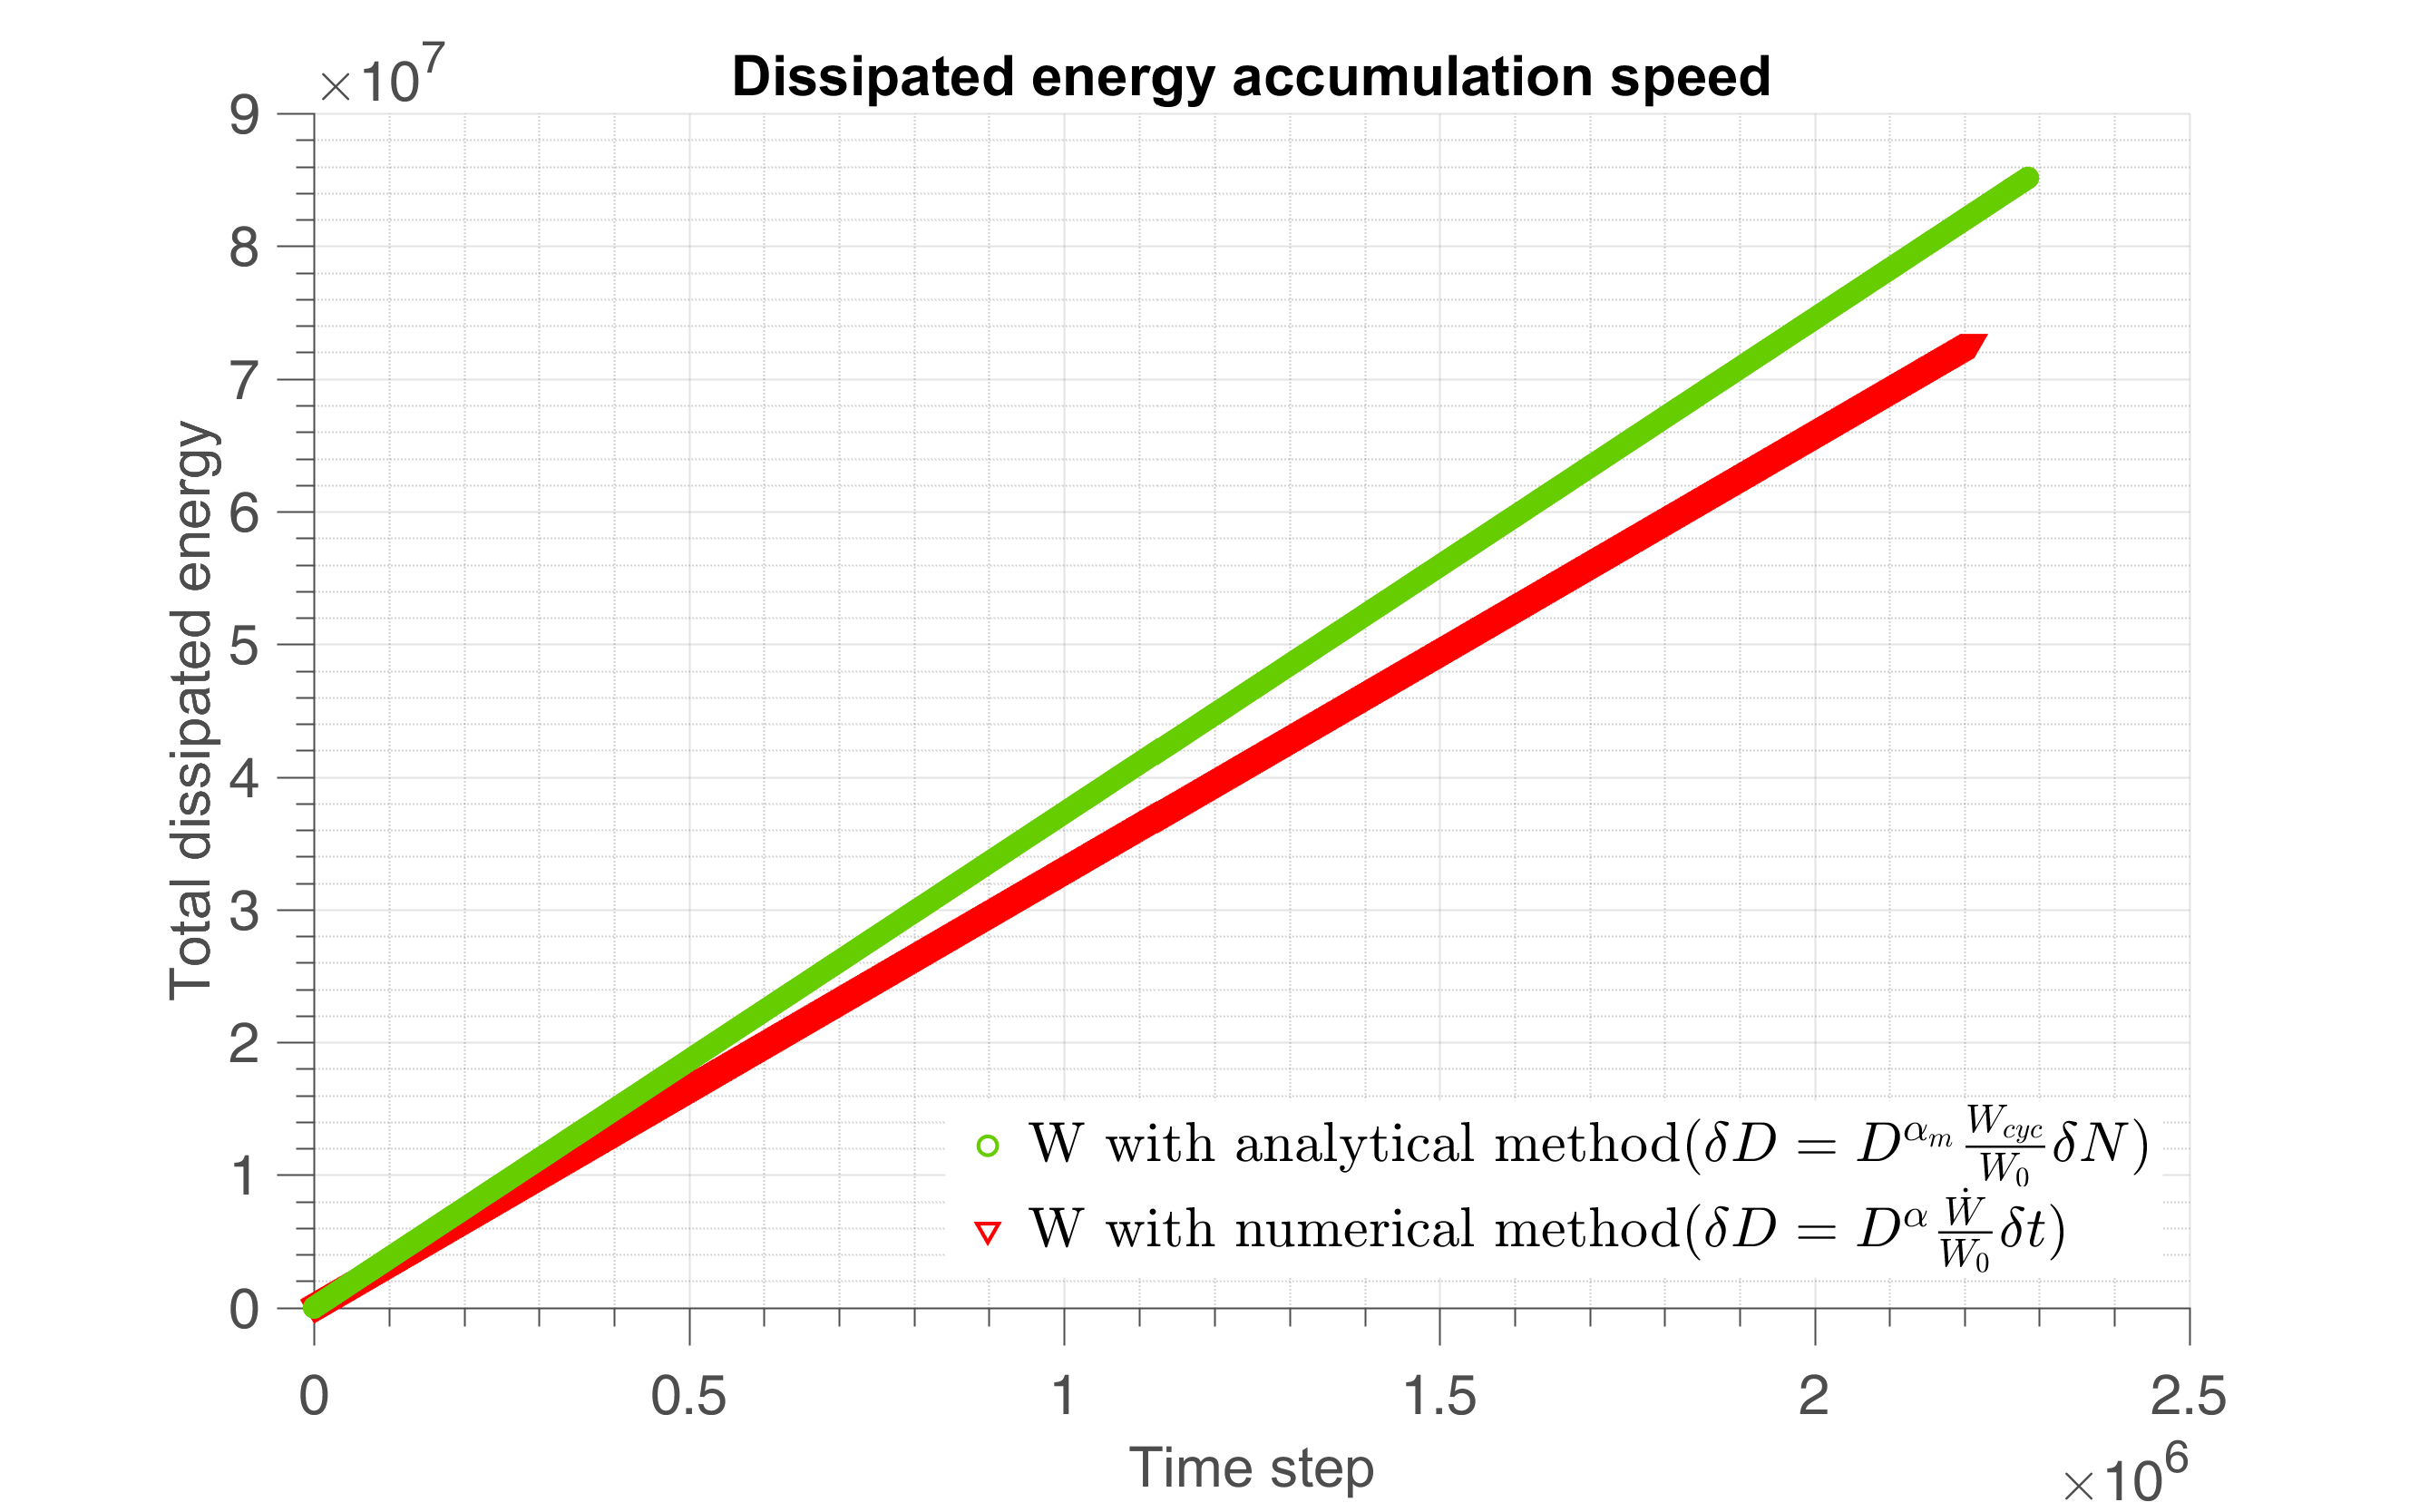
\includegraphics[width=0.95\textwidth]{figures//W3methods_bigbeta_04y.png} 
	\caption{Validation of dissipated energy in all scales with analytical and numerical method with $\beta=5$, $\Sigma=0.4\sigma_y$ }
	\label{fig.W3methods_bigbeta_04y}
\end{figure}
\begin{figure}[!h]
	\centering
	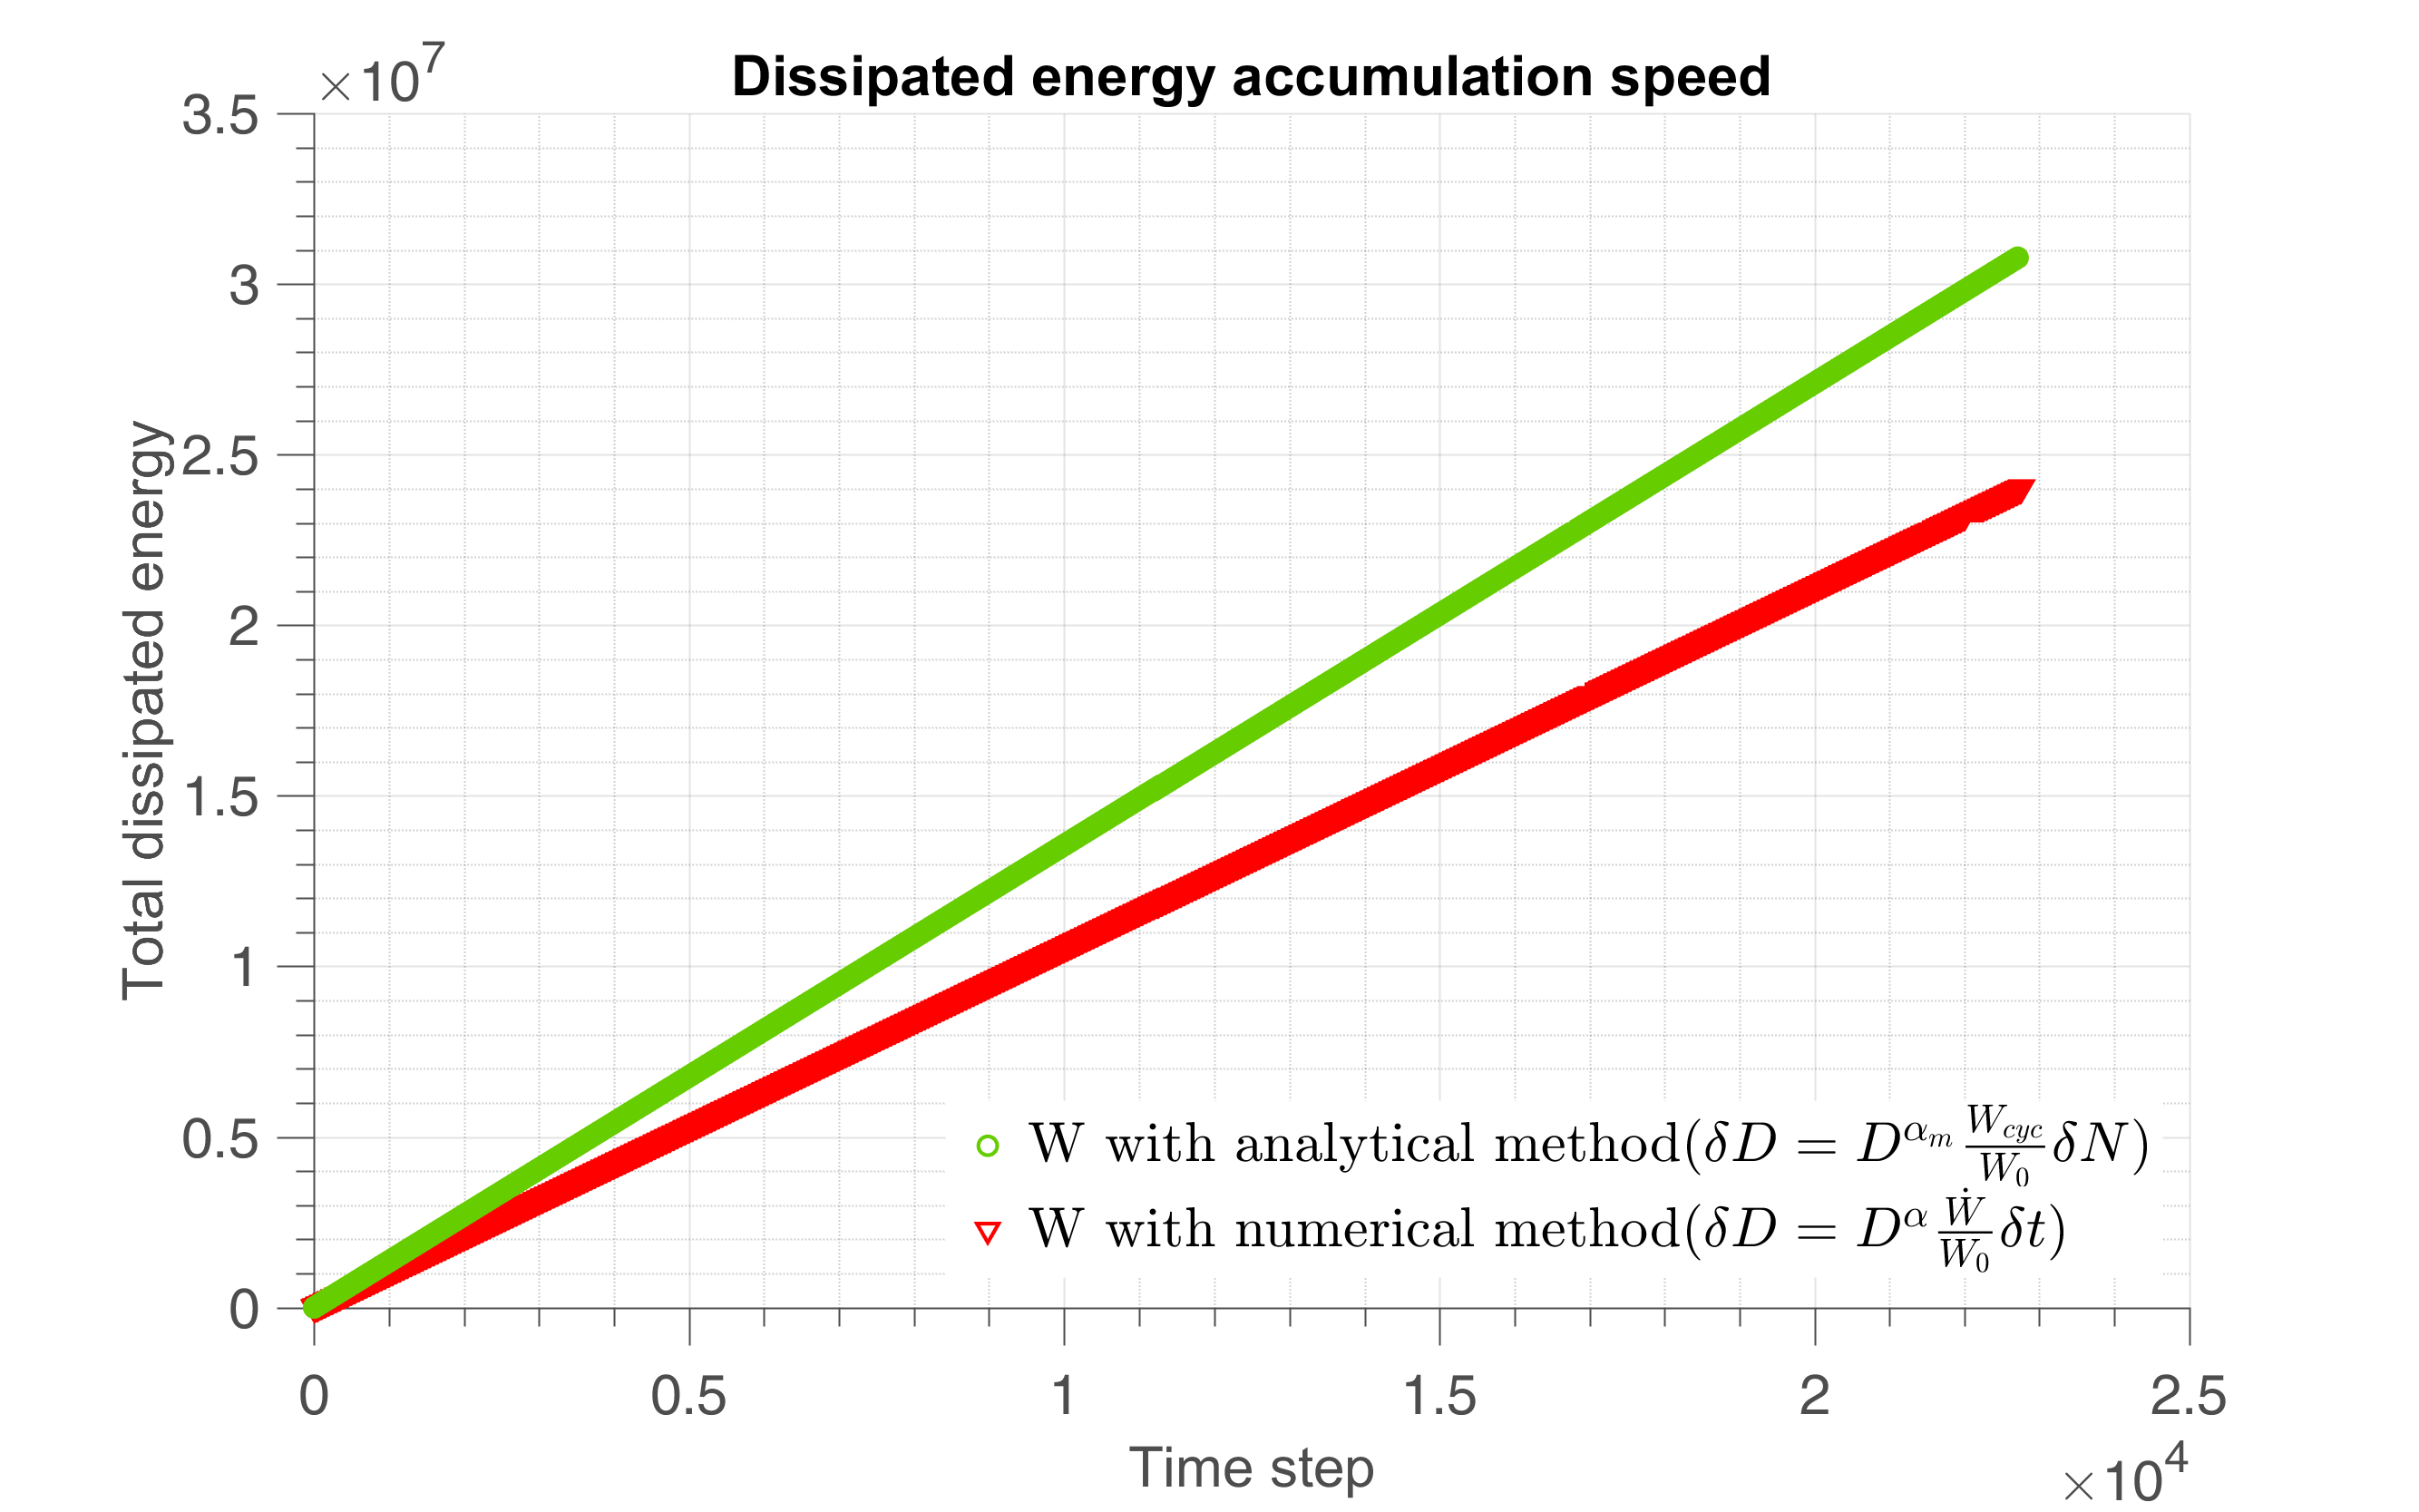
\includegraphics[width=0.95\textwidth]{figures//W3methods_bigbeta_08y.png} 
	\caption{Validation of dissipated energy in all scales with analytical and numerical method with $\beta=5$, $\Sigma=0.8\sigma_y$ }
	\label{fig.W3methods_bigbeta_08y}
\end{figure}
\begin{figure}[!h]
	\centering
	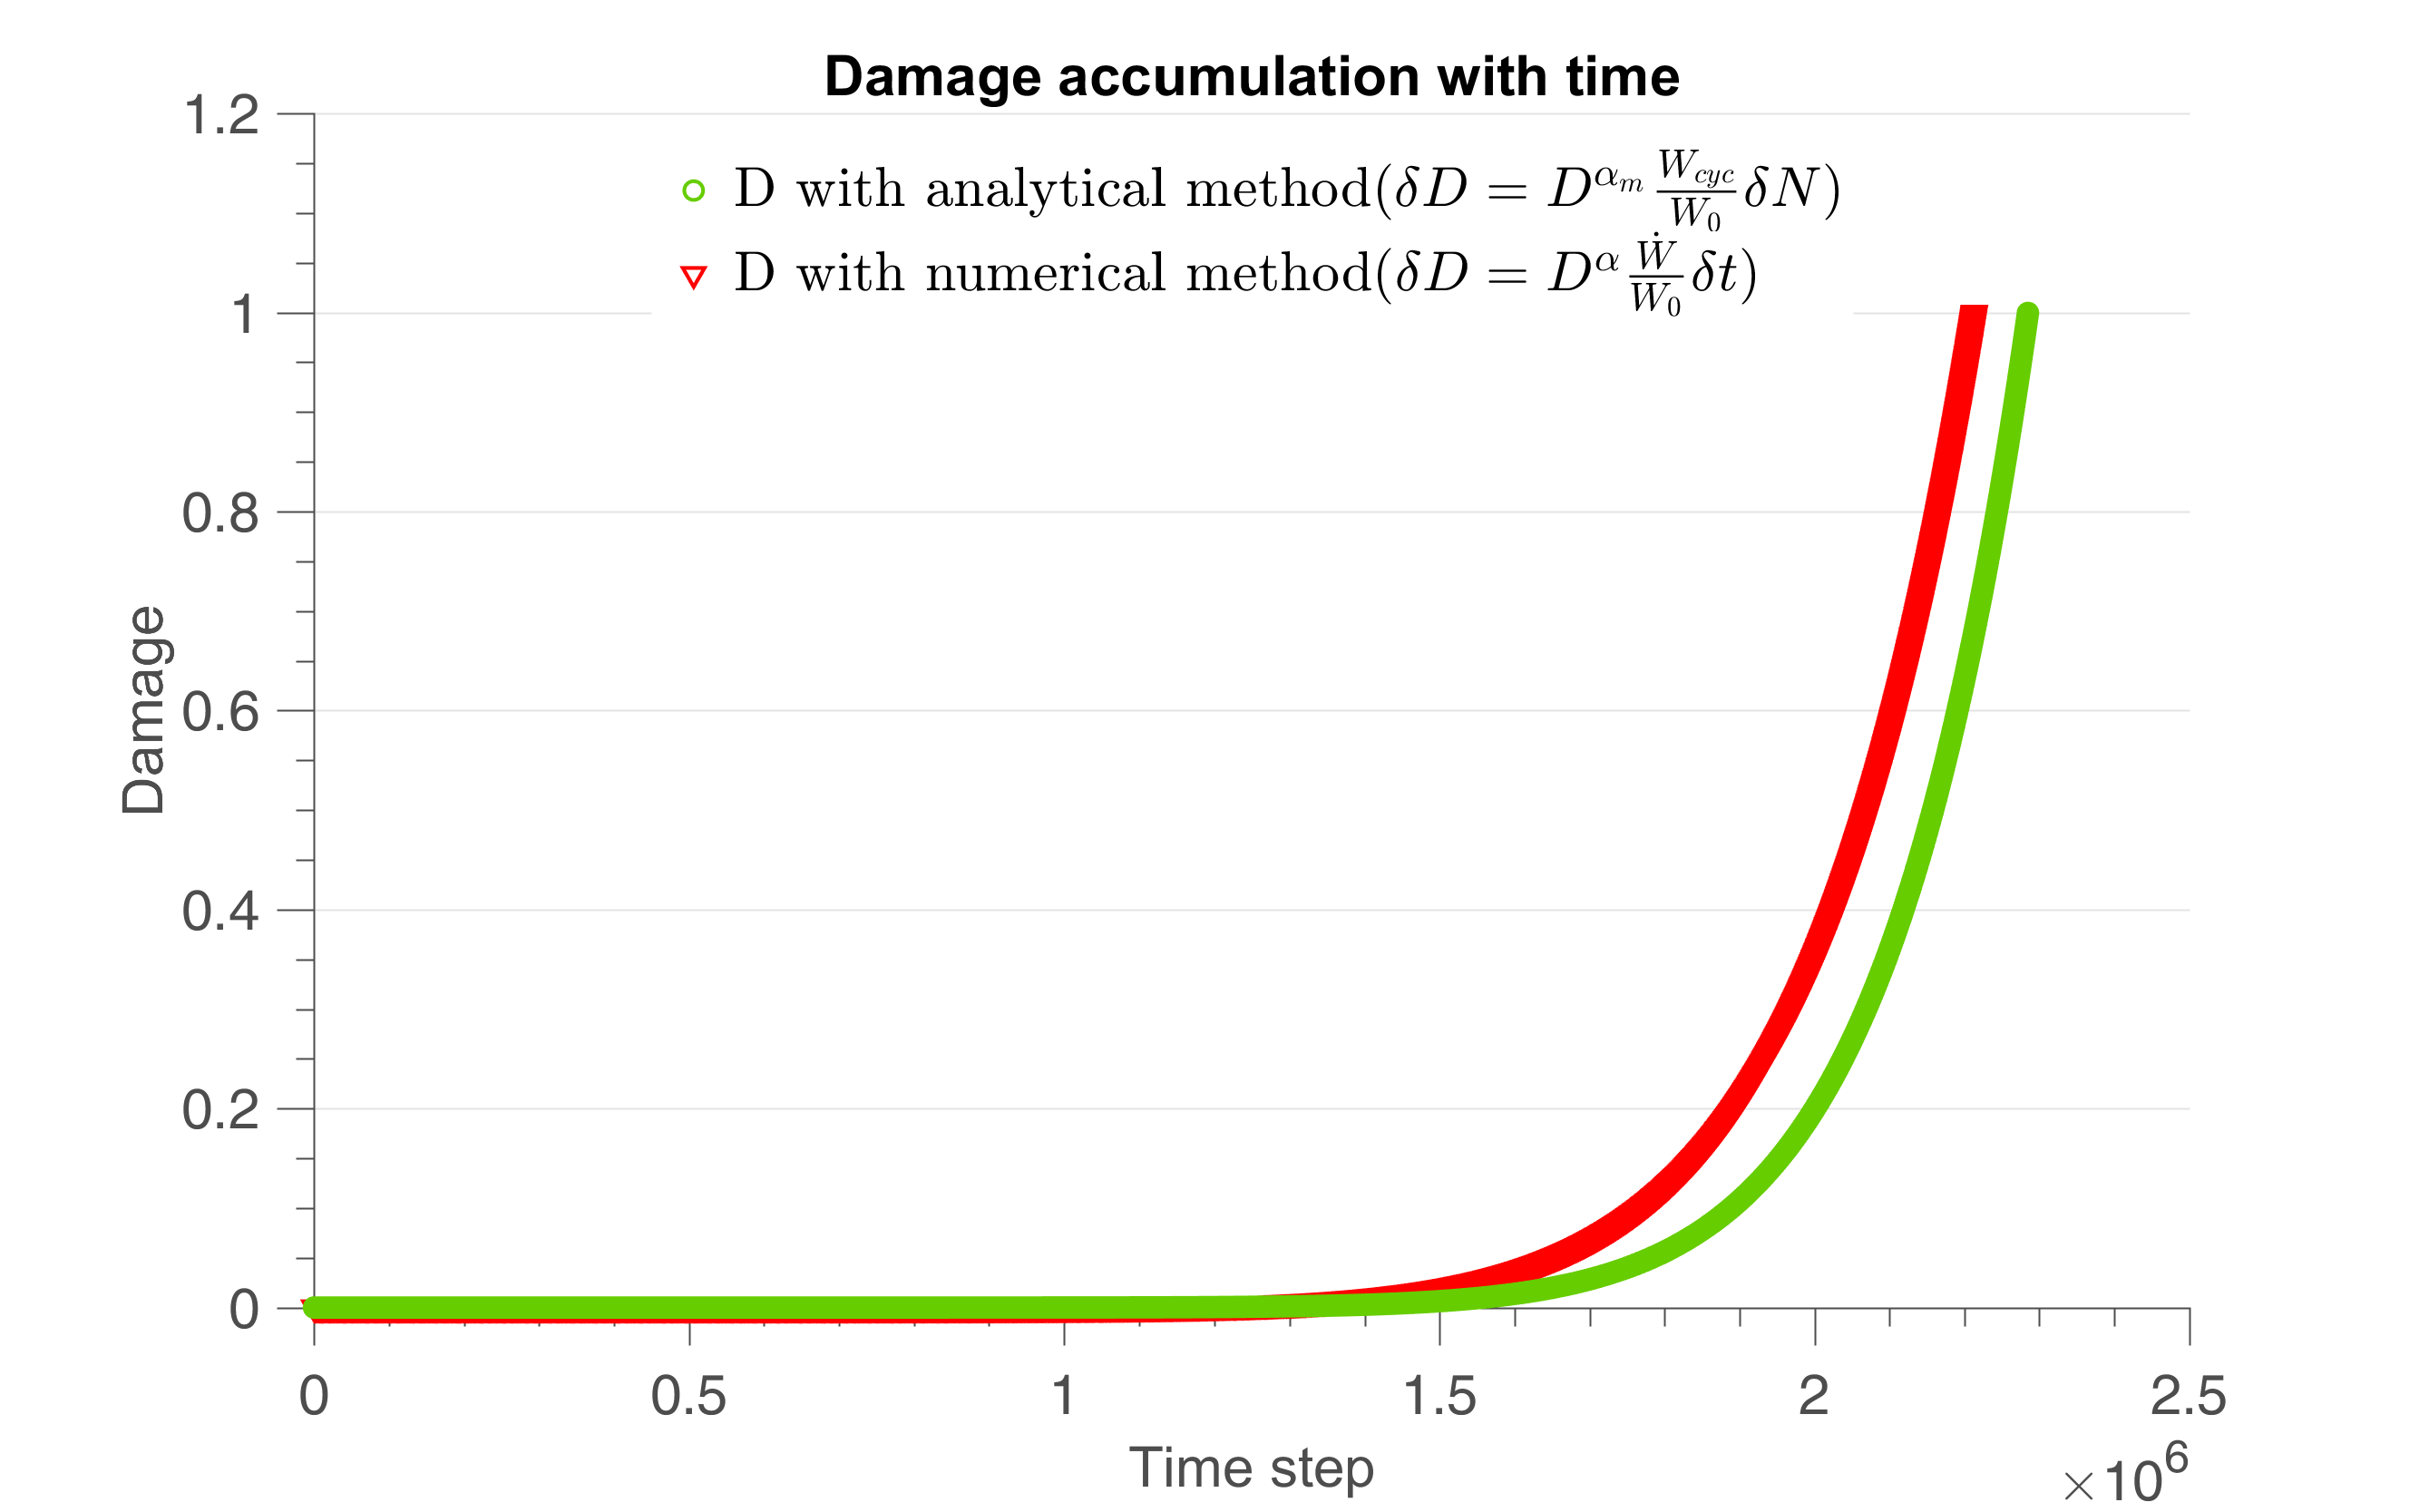
\includegraphics[width=\textwidth]{figures//damsin_bigbeta_04y.png} 
	\caption{Damage evolution with time under sinusoidal load with $\beta=5$, $\Sigma=0.4\sigma_y$. In such a severe loading and with extreme non-linearity, the simple Chaboche like formula with frozen $\alpha$ departs from the outcome of the full numerical model}
	\label{fig.damsin_bigbeta_04y}
\end{figure}
\begin{figure}[!h]
	\centering
	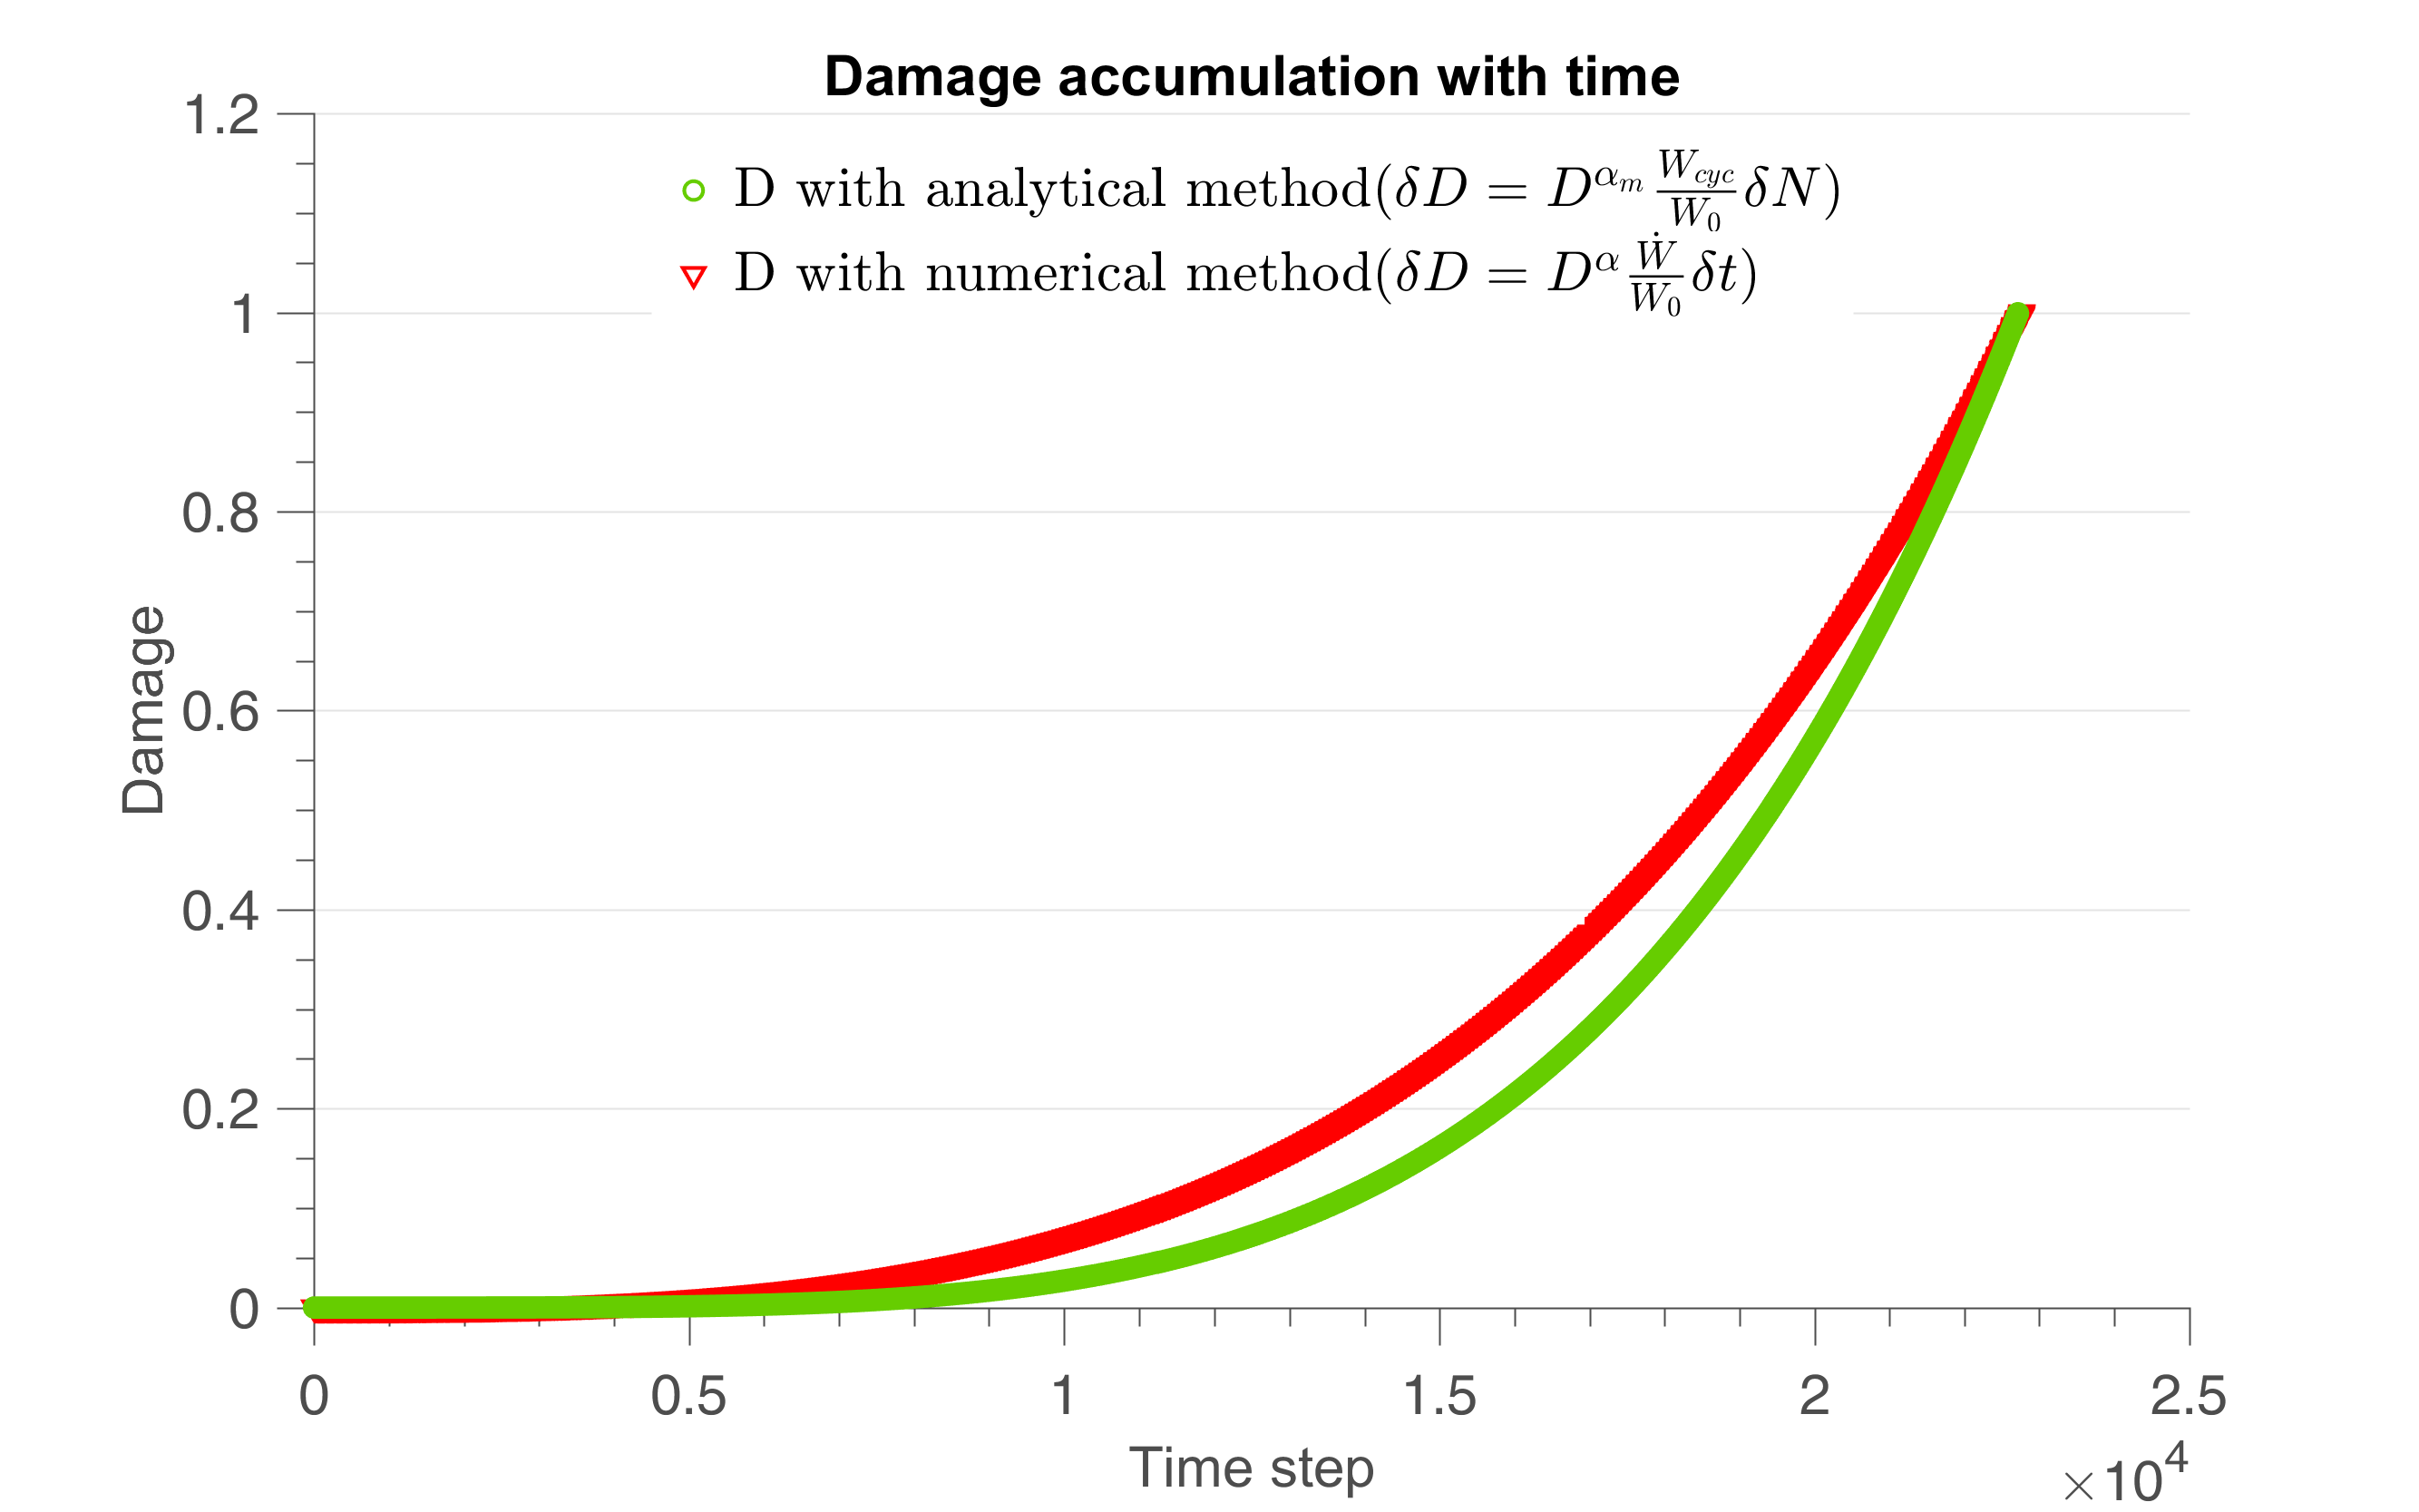
\includegraphics[width=\textwidth]{figures//damsin_bigbeta_08y.png} 
	\caption{Damage evolution with time under sinusoidal load with $\beta=5$, $\Sigma=0.8\sigma_y$}
	\label{fig.damsin_bigbeta_08y}
\end{figure}

\clearpage
\subsection{Numerical recovery of sequence effect}
We adopt the parameter $\alpha$ to take into account the sequence effect. The high-low loading sequence clearly reduces the fatigue life, as depicted in \figref{fig.sequencesigalpd}. In order to cover this phenomenon, we let $\alpha$ change with time($\alpha=1-a\left( s_{min}(t)-1\right)^{-f}$). Here $a$ is the sequence effect sensitivity. According to Eq.\eqref{eq.smin}, we have:
$$
s_{min}(t)=\dfrac{\Sigma_y-\lambda \Sigma_H(t)}{S_{a}(t)},
$$
which is the minimum weakening scale that activates energy loss.  We use a general law for $\alpha$ of the type $\alpha = \alpha (s_{min})$ with the idea that for us $s_{min}$ is a measure of present intensity of macroscopic stress. It is therefore a mechanical based stress norm. The impact of this construction of $\alpha$ can be seen on \figref{fig.randomdispersion}, on a test case specifically built to illustrate such a sequence effect.

\begin{Figure}[]{Two level sequence effect. By comparing the vertical figures we can see high stress gives high $(1-\alpha)$ value which causes fast damage accumulation speed. The evolution of $(1-\alpha)$ is highly nonlinear and follows the value of stress at each time step.}[fig.sequencesigalpd]
	\centerline{
		\graphfile*[40]{figures//high-low-Smax.png}[]
		\graphfile*[40]{figures//low-high-Smax.png}[]}
	\\
	\centerline{
		\graphfile*[40]{figures//high-low-alp.png}[]
		\graphfile*[40]{figures//low-high-alp.png}[]}
	\\
	\centerline{
		\graphfile*[40]{figures//high-low-D.png}[]
		\graphfile*[40]{figures//low-high-D.png}[]}
	\label{fig.sequencesigalpd}
\end{Figure}


\clearpage
\subsubsection{Major damage effect}

To see the influence of sequence effect factor of $\alpha$, we first fix $\alpha$ for all tests to see the results. When $\alpha$ is fixed, it becomes denominator in the final expression of $N_F$ (Eq.\eqref{eq.NFWcyc}) and has the same impact as $W_0$. We find  that the fatigue life of random loading is widely dispersed (\figref{fig.randomdispersion}). In this case we need to use $\alpha=f(s_{min})$ which evolves with time to make large stress intensity bring more damage.

\begin{figure}[!h]
	\centering
	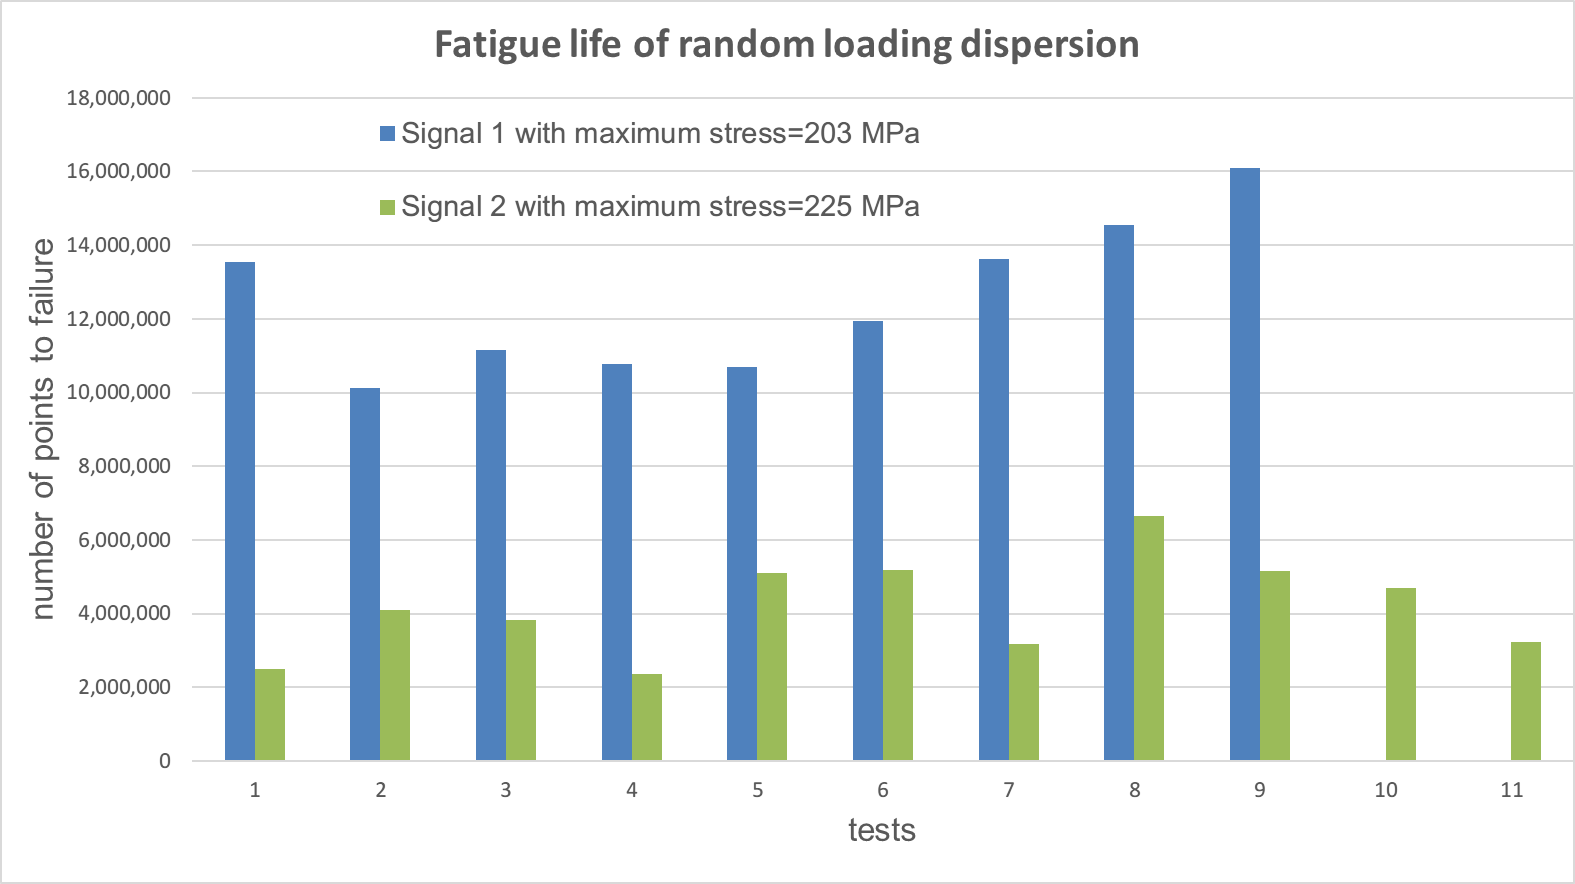
\includegraphics[width=\textwidth]{figures//randomdispersion.png} 
	\caption{Fatigue life of random loading dispersion}
	\label{fig.randomdispersion}
\end{figure}

After comparison with the experimental data we find out that large stresses cause much more damage than the smaller ones. It is necessary to include this major stress induced damage to our stress intensity parameter $\alpha$. With the new $\alpha$ used in Eq.\eqref{eq.final3} compared to Eq.\eqref{eq.alpha} we are able to calibrate our model better with the experimental results by using 
\begin{equation}
\alpha=1-a\left(  \dfrac{\frac{1}{s_{min}}}{1-\frac{1}{s_{min}}} \right) ^{f}.
\label{eq.majoralp}
\end{equation}


With $f=1.1$, we use the power to magnify large stress impact and minify lower stress damage.  The demonstration of major damage effect using magnification power is depicted in \figref{fig.sequenceours}. With larger value of power, the sequence effect is more significant(bigger dispersion between high-low and low-high sequence).

\begin{figure}[!h]
	\centering
	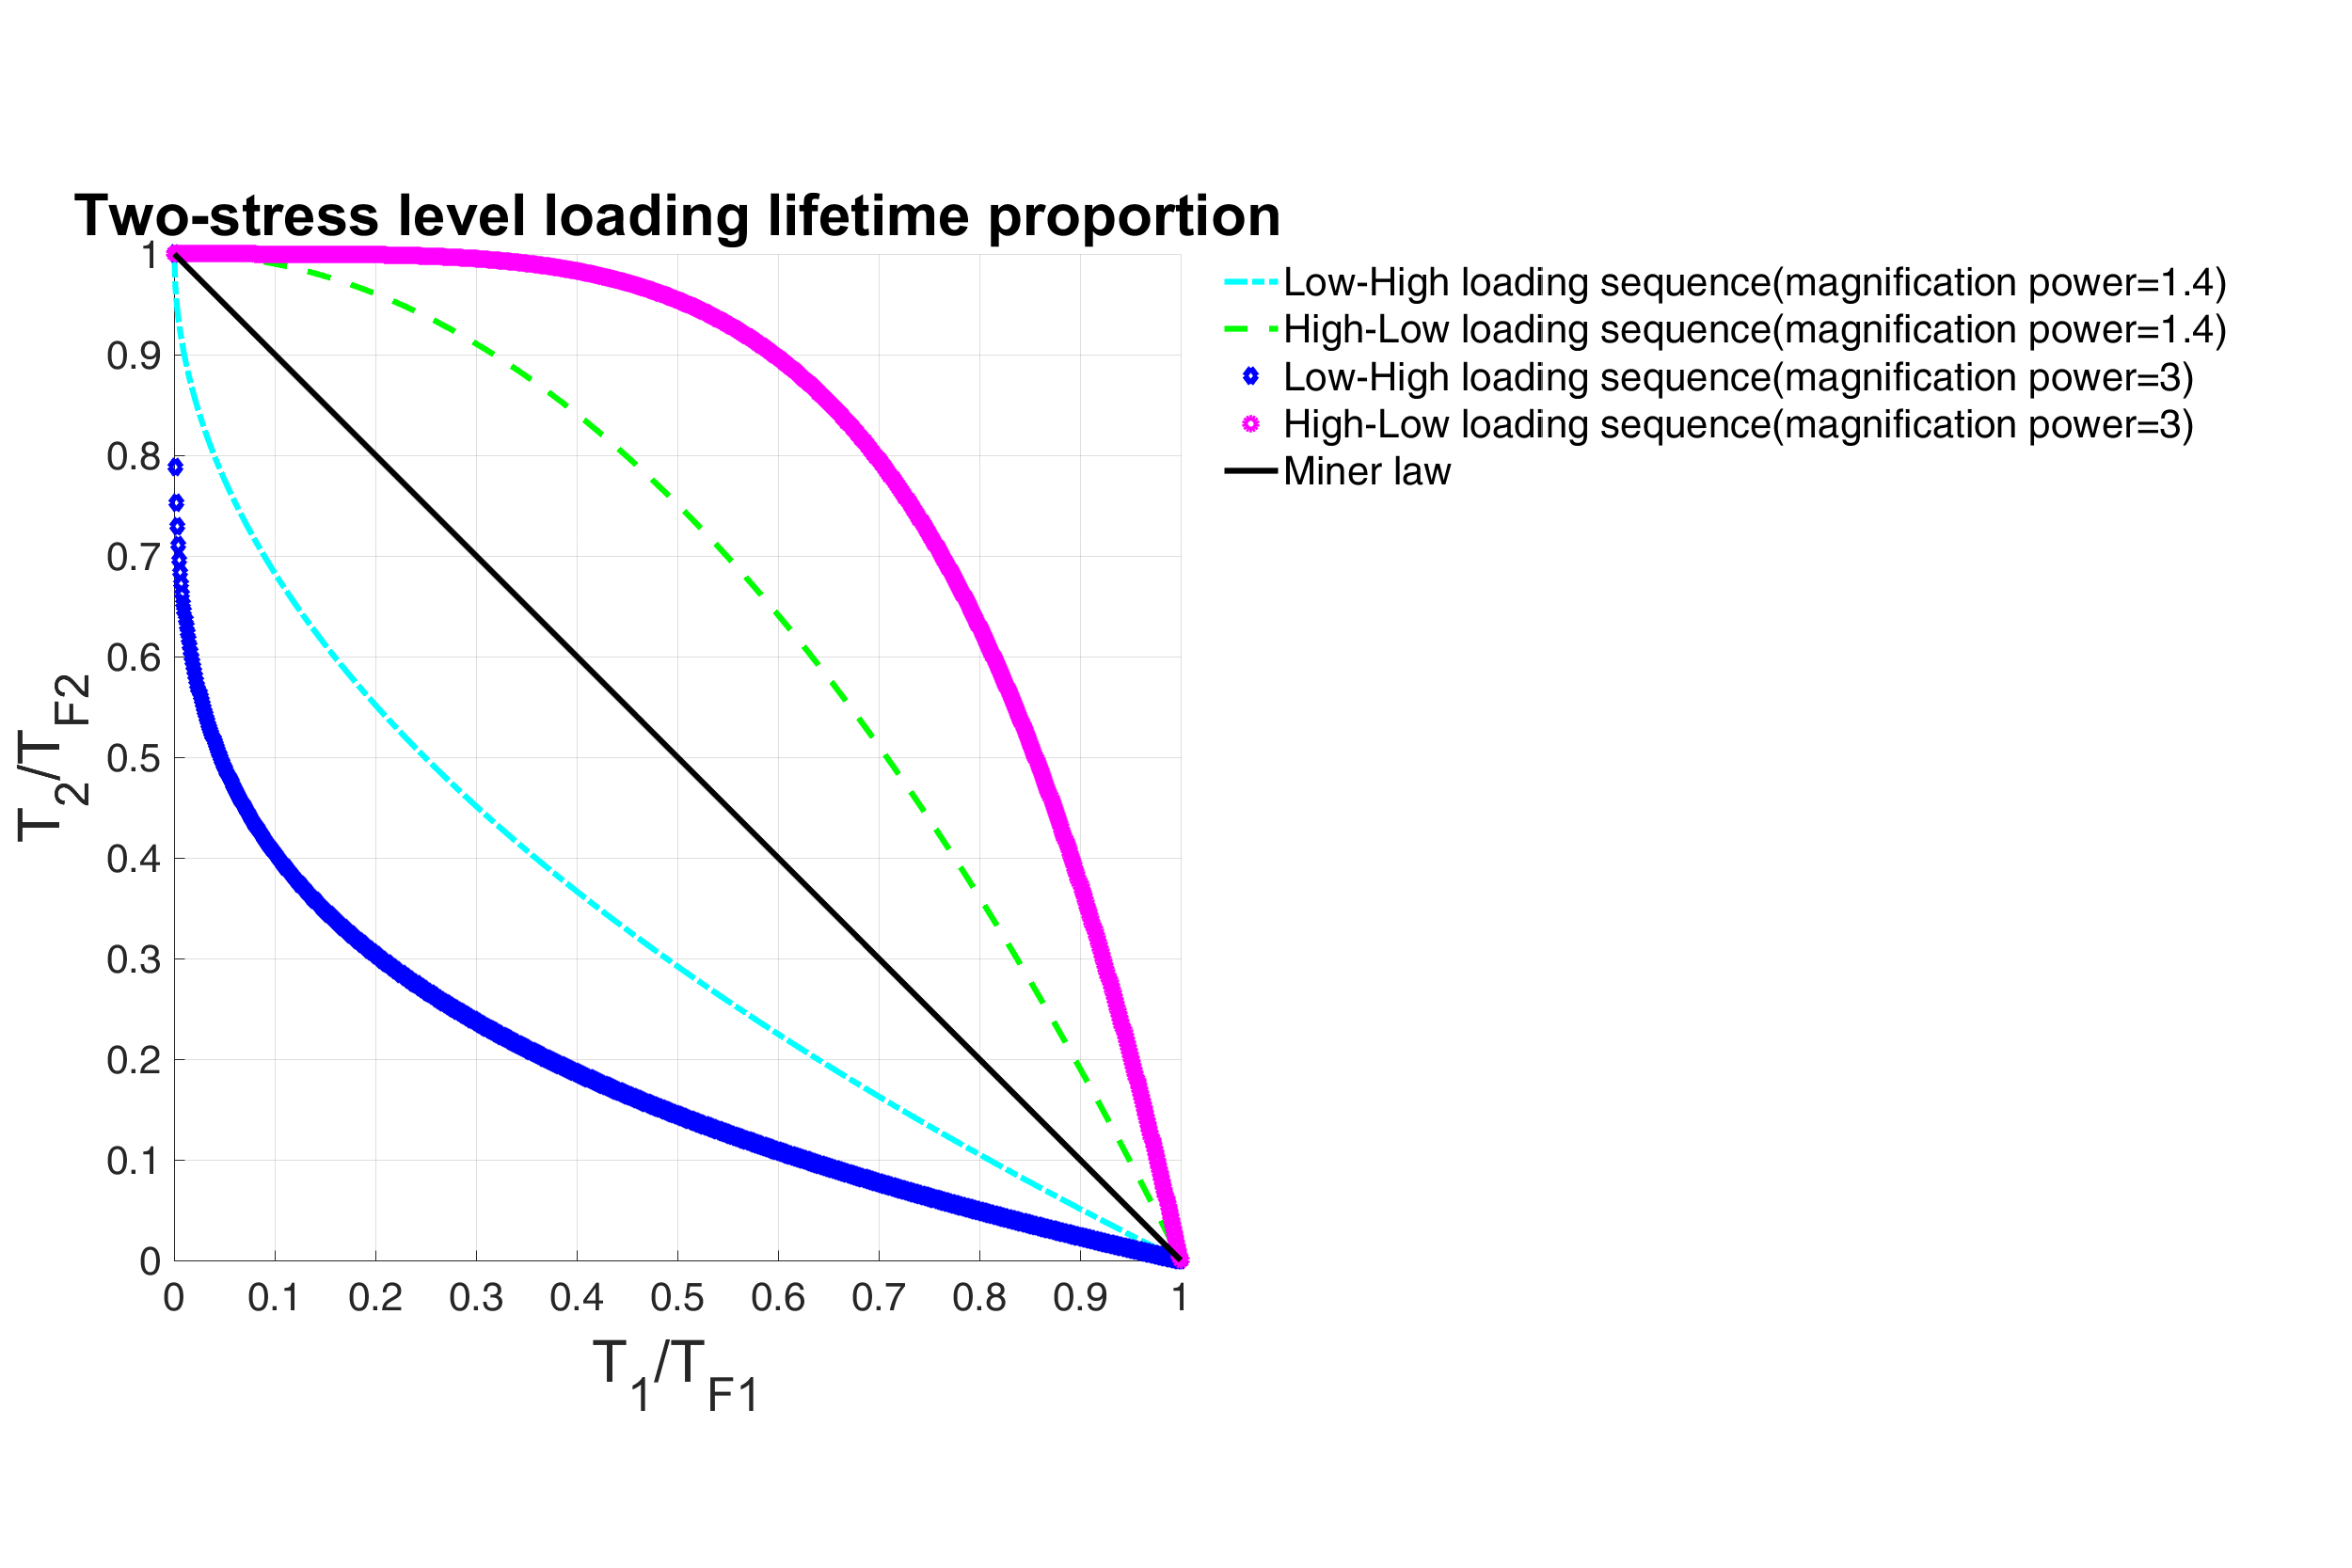
\includegraphics[width=\textwidth]{figures//sequence_ours.png} 
	\caption{Major damage effect using different magnification power of Eq.\eqref{eq.majoralp} on sequence effect. Here high stress is 1MPa and low stress is 0.8MPa. We see that using a large power $f$ in Eq.\eqref{eq.majoralp} induces a stronger sequence effect.}
	\label{fig.sequenceours}
\end{figure}

The larger value of $S_{a}$ causes more damage in the presence of the power $\beta$, leading to faster increase of 
$$(1-\alpha)=a\left(  \dfrac{\frac{1}{s_{min}}}{1-\frac{1}{s_{min}}} \right) ^{f}=a(s_{min}-1)^{-f}.$$ 
which causes faster damage accumulation. We can also see this effect in \figref{fig.SmaxSequence}. 

To assess large stress correctly we define the larger stress intensity as the value of stress which makes expression in the bracket in the second term of $\alpha$ greater than 1($ \dfrac{1}{ s_{min}(t)-1 }>1$), then we use power $\beta$ to magnify this term. In this way the damage is accelerated for large stresses. The deviatoric stress $S_{a}$, above which the damage is magnified,  is determined from: 
$$\alpha(t)=1-a\left( \dfrac{1}{ s_{min}(t)-1 } \right)^{1.1},$$
$$s_{min}(t)=\dfrac{\Sigma_y-\lambda \Sigma_H(t)}{S_{a}(t)}<2,$$
$$S_{large}(t)>\dfrac{\Sigma_y-\lambda \Sigma_H(t)}{2}.$$ 

The major damage effect can be seen in \figref{fig.SmaxSequence}, which occurs when $S$ is more than half the macroscopic yield stress of the material.

\begin{figure}[!h]
	\centering
	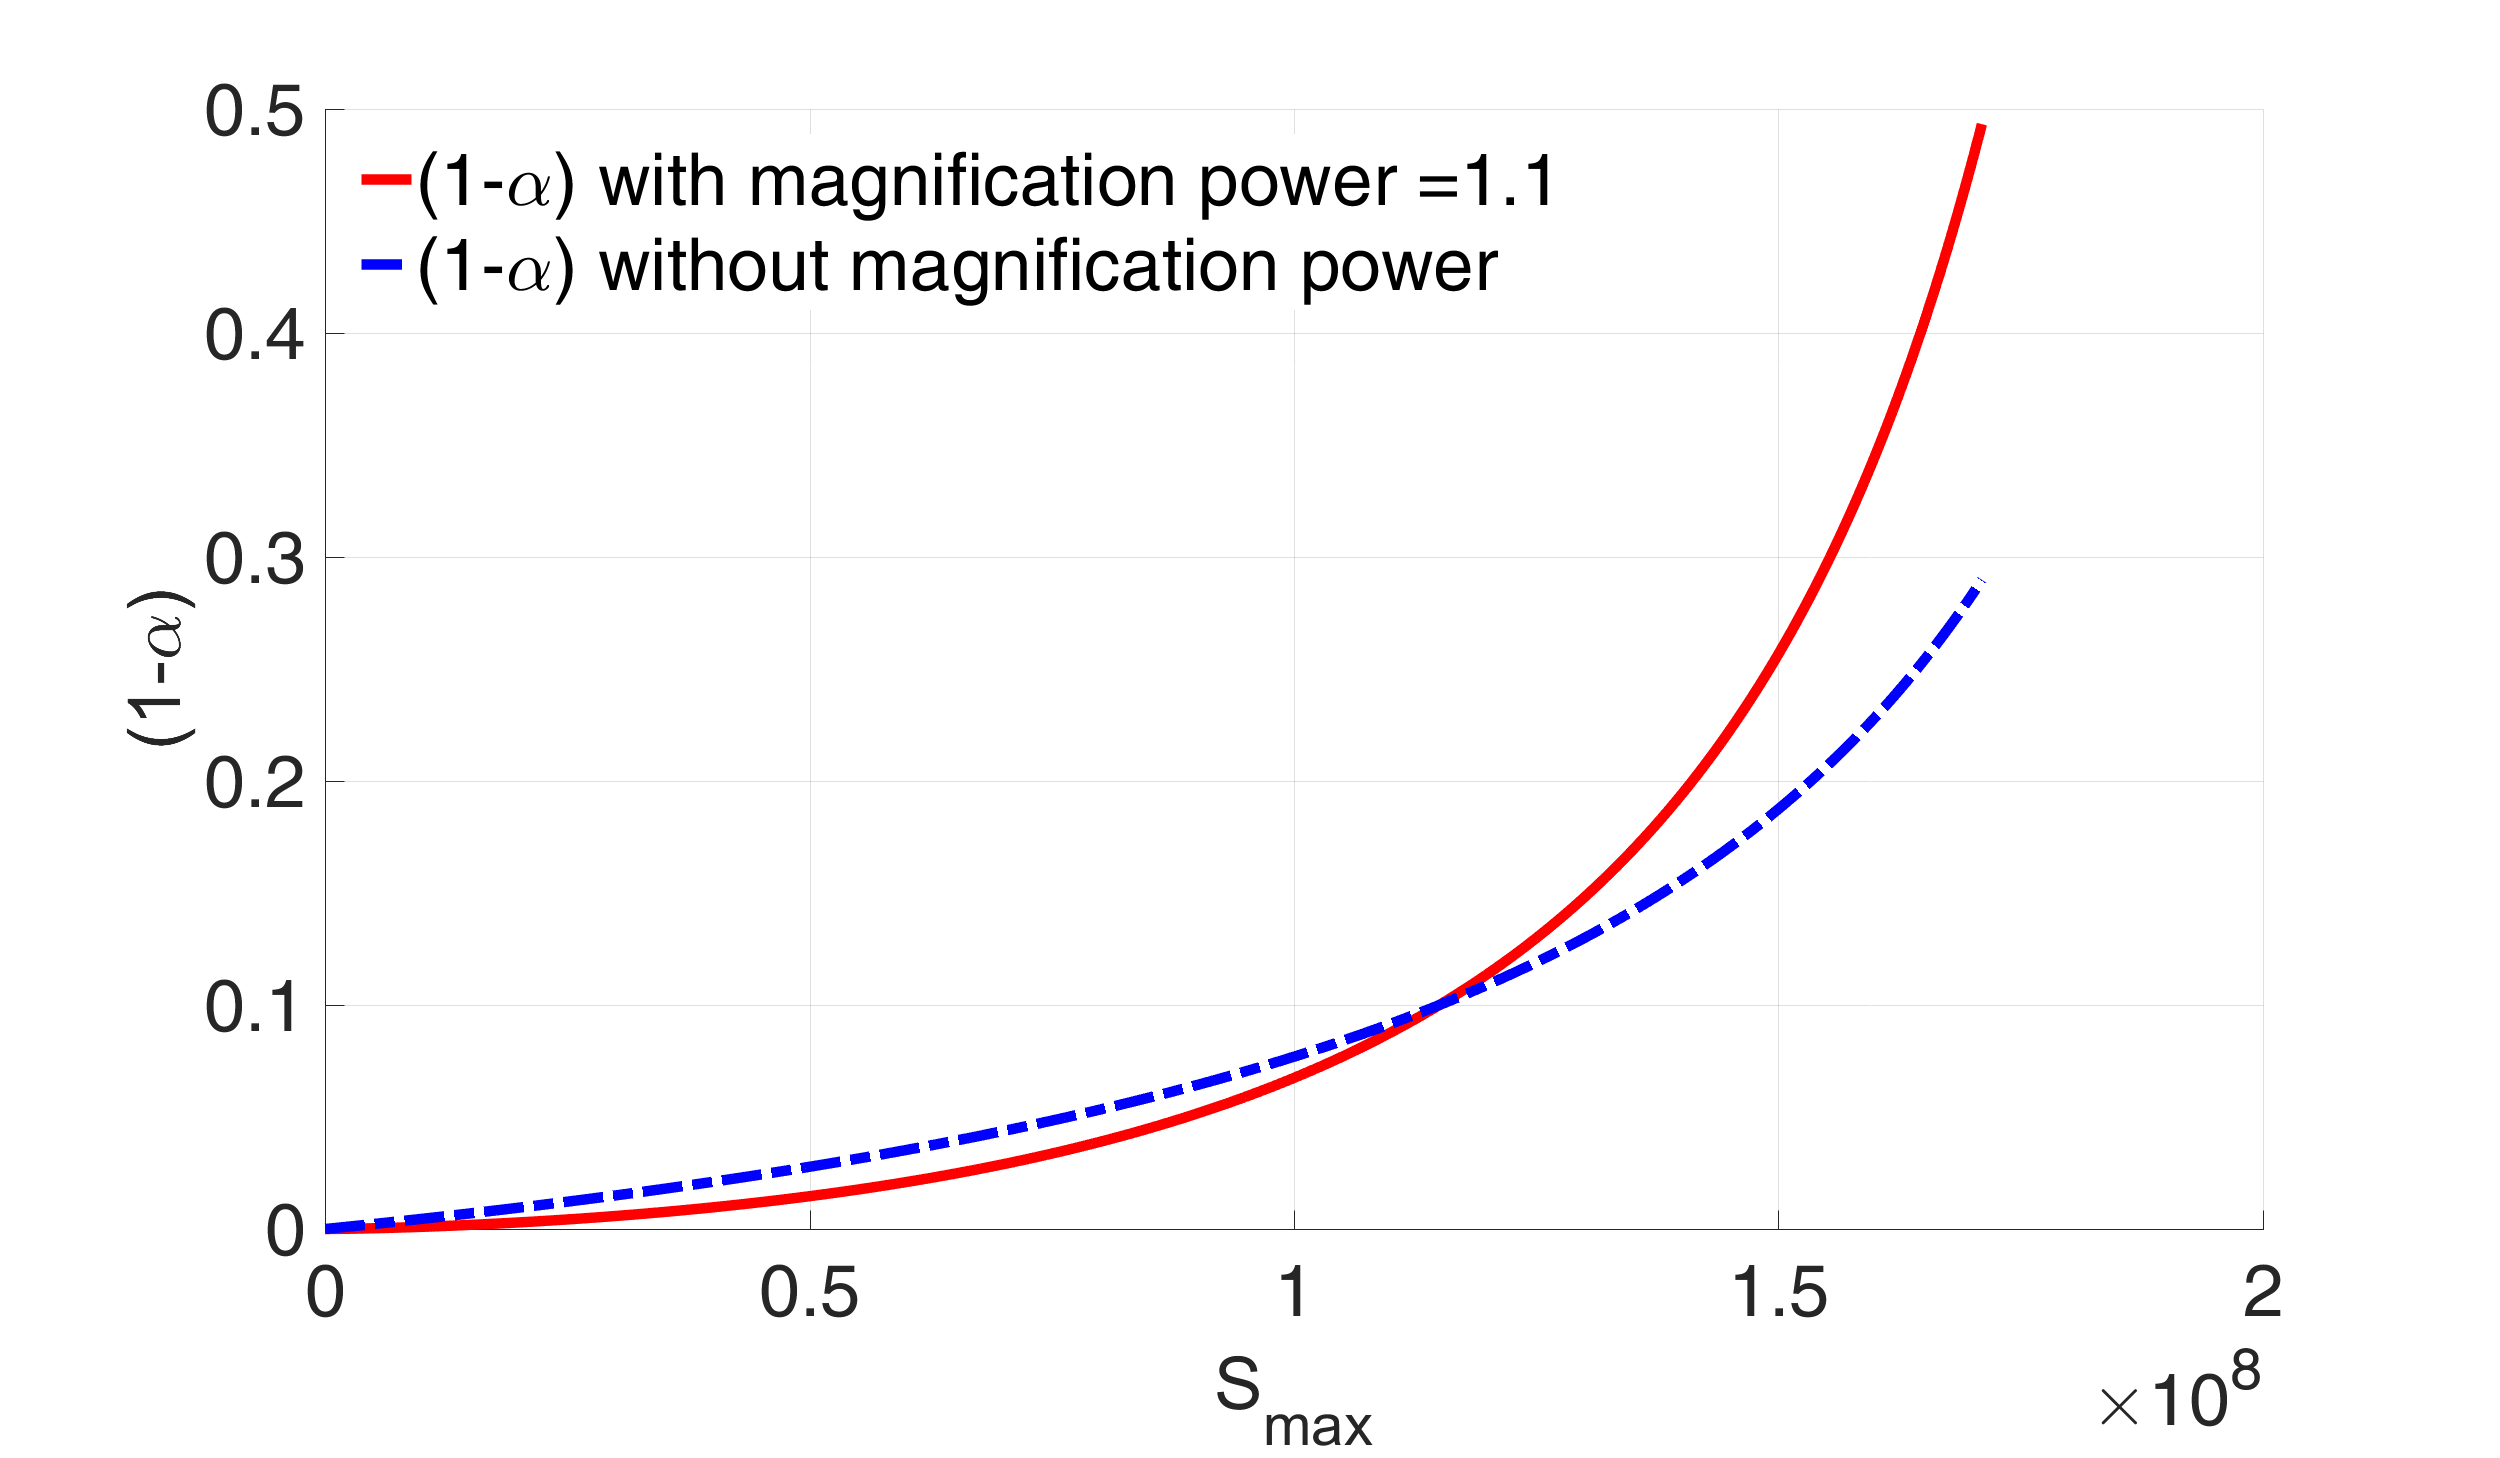
\includegraphics[width=\textwidth]{figures//alp_Smax_fb.png} 
	\caption{(1-$\alpha$) term which stands for the load intensity evolution, both with and without the magnification power $f$}
	\label{fig.SmaxSequence}
\end{figure}

\clearpage
\section{Identification strategy}
\label{sec:5.9}
In our tests we keep $f=1.1$(justified in Chapter \ref{chp:6} by \figref{fig.Cetimerralpfix} and \figref{fig.Cetimerr}). The positive hydrostatic stress and negative one have different effect on the yield limit. It is necessary to adopt 2 parameters to describe this behavior. So we divide the hydrostatic sensitivity $\lambda$ into 2 parts. $\lambda_+$ and $\lambda_-$. In the analytical formula, the amplitude of the stress intensity is adopted and the average value of tension hydrostatic stress(+) and compressive hydrostatic stress(-) is introduced.

For a good lifetime prediction, it is necessary to first identify the appropriate parameters of the model. For this purpose, we use the analytical formula Eq.\eqref{eq.cycNF} obtained in uniaxial cyclic loading case. With distinction of the hydrostatic stress in the presence of non-zero mean stress and since in fully reversed uniaxial loading we spend an equal time in compression and in traction, Eq.\eqref{eq:w} now writes:

\begin{equation}
W_{cyc}=\dfrac{2(E-k)(1+\nu)\left( \beta-1\right) }{ E(E+k\nu)\beta\left( \beta+1\right) }\left[ \dfrac{S_{a}^{\beta+1}}{ \left(\sigma_y-\lambda_+ \overline{\Sigma}_{H+}(t)\right)^{\beta-1}}+\dfrac{S_{a}^{\beta+1}}{ \left(\sigma_y-\lambda_- \overline{\Sigma}_{H-}(t)\right)^{\beta-1}}\right] .
\label{eq:wcycnew}
\end{equation}

\begin{equation}N_{Fnum}=\dfrac{W_0}{\left( 1-\alpha\right) }\dfrac{E(E+k\nu)\beta\left( \beta+1\right) }{ 2(E-k)(1+\nu)\left( \beta-1\right) }\dfrac{1}{\dfrac{S_{a}^{\beta+1}}{\left(\sigma_y-\lambda_+\overline{\Sigma}_{H+}(t)\right)^{\beta-1}}+\dfrac{S_{a}^{\beta+1}}{\left(\sigma_y-\lambda_-\overline{\Sigma}_{H-}(t)\right)^{\beta-1}}}.\label{eq:NFnew}
\end{equation}


To use our analytical model Eq.\eqref{eq:NFnew} to fit the experiments, we employ matlab Least-Squares (model fitting) algorithm. 

The best fitted parameters in uniaxial cyclic loading case are deduced from the minimization of the sum of square of difference between uniaxial numerical and experimental results:
\begin{equation}
\min_{\beta,\lambda,W_0}\left\lbrace \sum_{i}\left(N_{Fnum}-N_{Fexp} \right)^2\right\rbrace 
\label{eq.leastsquares}
\end{equation}

Assume there are $i$ sets of experimental data. To clarify the identification process, let us separate the parameters into:
\begin{itemize}
	\item Experimental data: $S_{a(i)}$, $\Sigma_{H(i)}$, $N_{Fexp(i)}$, $\sigma_y$, $E$, $k$, $\nu$.
	\item Material constants: $\beta$, $\lambda_{+-}$, $W_0$ (to be fitted)
	\item Input data from experimental data: $S_{max(i)}$, $\Sigma_{H(i)}$
	\item Input data from experimental data and parameter constants: $\alpha_{(i)}$
	\item Output data: $N_{Fnum(i)}$
\end{itemize}

In this process, $\sigma_y$, $E$, $k$ and $\nu$ are given elastoplastic material constants. For each test (i), the load parameters are maximum amplitude $S_{a(i)}$, mean hydrostatic stress $\overline{\Sigma}_{H(i)}$, and the experimental number of cycles to failure is given by $N_{Fexp(i)}$.

The exponent $\alpha_{(i)}$ is cycle average obtained by
\begin{equation}
\alpha_{(i)}=mean\left[1-a\left( \dfrac{1}{\dfrac{\Sigma_y-\lambda_{+-} \Sigma_{H}(t)}{S_{a}(t)}-1 } \right)^{1.1}\right] (i).
\label{eq.meanalp}
\end{equation}

The parameters to be calibrated are $W_0$, $\beta$ and $\lambda$. Since the exponent $\alpha_{(i)}$ depends on $\beta$ and $\lambda$, we proceed iteratively by:

\begin{enumerate}
	\item We first identify the S-N curve slope $\beta$ and the energy scale $W_0$ using the analytical formula with torsion tests because there is no $\lambda_{+-}$ impact in this kind of loading. We start from an initial guess $\beta$ from which we can deduce $\alpha_{(i)}$ by  numerical calculation of Eq.\ref{eq.meanalp} and identify $\beta$ and $W_0$ by least squares. Because our analytical formula is not derivable in all ranges, when the identified value of $\beta$ or $W_0$ get stuck in local minimum value, we regenerate a random $\beta$ or $W_0$ in their range so as to get the global least square value.
	\item Then, the parameter $\lambda_{+}$ are identified from numerical bending tests and we keep $\lambda_-=0$. The final parameters correspond to the $\lambda$ leading to the lowest identification error in $\beta$ and $W_0$. This strategy handles the nonlinearity in $\beta$ and is well adapted to the low sensitivity in $\lambda$.
\end{enumerate}



The analytical formula Eq.\eqref{eq:NFnew} with mean stress effect converges with the numerical method very well in the case of small $\beta$ and $\lambda_{+-}$. 


\textbf{Parameter sensitivity analysis}

The parameters we introduced during the deduction need to be calibrated. The source of the parameter identification are listed in Table.\ref{paras}.
We perform a sensitivity analysis to see the influence of each parameter by comparing the results obtained respectively for the reference value, an upper bound and a lower bound of each parameter.

\begin{table}[!h]
	\centering
	\begin{tabular}{l|c}
		\hline
		\textbf{Parameters}                                  & \multicolumn{1}{c}{\textbf{Strategy}} \\ \hline
		Hydrostatic pressure sensitivity $\lambda_+$           & hydrostatic stress sensitivity (identified)         \\
		Non-linearity of damage accumulation  $a$        & amplification factor of load intensity (guessed)     \\
		Weakening scales distribution exponent  $\beta$      & to be calibrated (identified)                   \\
		Dissipated energy to failure per defect  $W_0$ & energy scaling (identified)              \\ \hline
	\end{tabular}
	\caption{Parameters concerned}
	\label{paras}
\end{table}

We analyze the sensitivity of parameters separately as in Table.\ref{tab.sensitivity_const1}(uniaxial) and Table.\ref{tab.sensitivity_random1}(random loading). The parameter $\beta$ has more influence on the random loading case because it acts not only as the S-N curve slope but also the power magnification factor of large stress intensity. The $\lambda$ has little influence because both tests are conducted on very small or zero mean stress load history.


In Miner's law the parameter $\alpha$ is zero, the maximum value is below 1. For $\alpha=1$ the damage accumulation line becomes flat and there will be unlimited lifetime. To keep $\alpha$ in the range of $[0,1]$ where in random amplitude tests there is $S_{a}=163.3MPa$; we set the sensitivity of load intensity  $a$  to a maximum value of $0.29$ to keep $\alpha$ positive. 

The weakening scale distribution exponent(also the slope of S-N curve of the material) $\beta$ ranges from $1$ to $5$. The hydrostatic pressure sensitivity $\lambda$ is from positive mean stress test, which has the range of $0\sim0.8$. In constant amplitude cyclic loading, the dissipated energy to failure per defect $W_0$(in MPa) is related to fatigue lifetime of the material.

\begin{table}[!h]
	\centering
	\begin{tabular}{lrrrrrrr}
		\hline
		\multicolumn{8}{c}{\textbf{Constant amplitude sensitivity test with $f(\beta)=\beta$}}                                                                                                                                                                                                                                           \\ \hline
		& \multicolumn{1}{r}{\textbf{Ref}} & \multicolumn{1}{r}{\textbf{Min}} & \multicolumn{1}{r}{\textbf{Max}} & \multicolumn{1}{r}{\textbf{Ref\_n}} & \multicolumn{1}{r}{\textbf{Min\_n}} & \multicolumn{1}{r}{\textbf{Max\_n}} & \multicolumn{1}{r}{\textbf{Sensitivity}} \\ \hline
		\textbf{$\beta$}   & 1.1                                          & 1.05                             & 1.50                             & 414233                                     & 
		783723 	                              & 243300 
		&-3.19 
		\\
		\textbf{$\lambda_+$} & 0.1                                          & 0.05                             & 0.50                             & 414233                                    & 449598 
		& 443376 
		& 0.00                                    \\
		\textbf{$W_0$}     & 3.27e8                                     & 1.00e8                         & 5.00e8                         & 414233                                     & 137498 
		& 687209 
		& 1.08                                    \\
		\textbf{$a$}       & 0.1                                          & 0.05                             & 0.15                             & 414233                                  & 672869 
		& 324754 
		& -0.84                                   \\ \hline
	\end{tabular}
	\caption{Example of parameters sensitivity at cyclic loading of BATCH\_A\_02 on AW-6106 T6 aluminum (table.\ref{tab:Cetim})}
	\label{tab.sensitivity_const1}
\end{table}

\clearpage

\section{Experimental verification}

\subsection{Introduction}
The aim of this chapter is to validate the predictive model proposed. This consists in simulating tests available in the literature to determine the lifetime at initiation of crack by the application of the model and to compare these with the experimental lifetimes. The validation of the model involves a wide variety of metallic materials. The loads tested are of two types: cyclic loading of multiaxial stress of constant amplitude and repeated sequences of uniaxial stresses of variable amplitudes. The fatigue data of the materials used and the loads tested are taken from laboratory experiments or the literature.

\subsection{Random amplitude 1D tests from Cetim on AW-6106 T6 aluminum}

What makes automobile fatigue so difficult to predict is that, unlike standard tests done in a laboratory, an automobile's structure has to endure a complex, mostly random, set of static as well as cyclical stresses when in service. For example in \figref{complexloading} which could represent load data from testing or measurement, extracting the cyclic information can be challenging. 
\begin{figure}[!h]
	\centering
	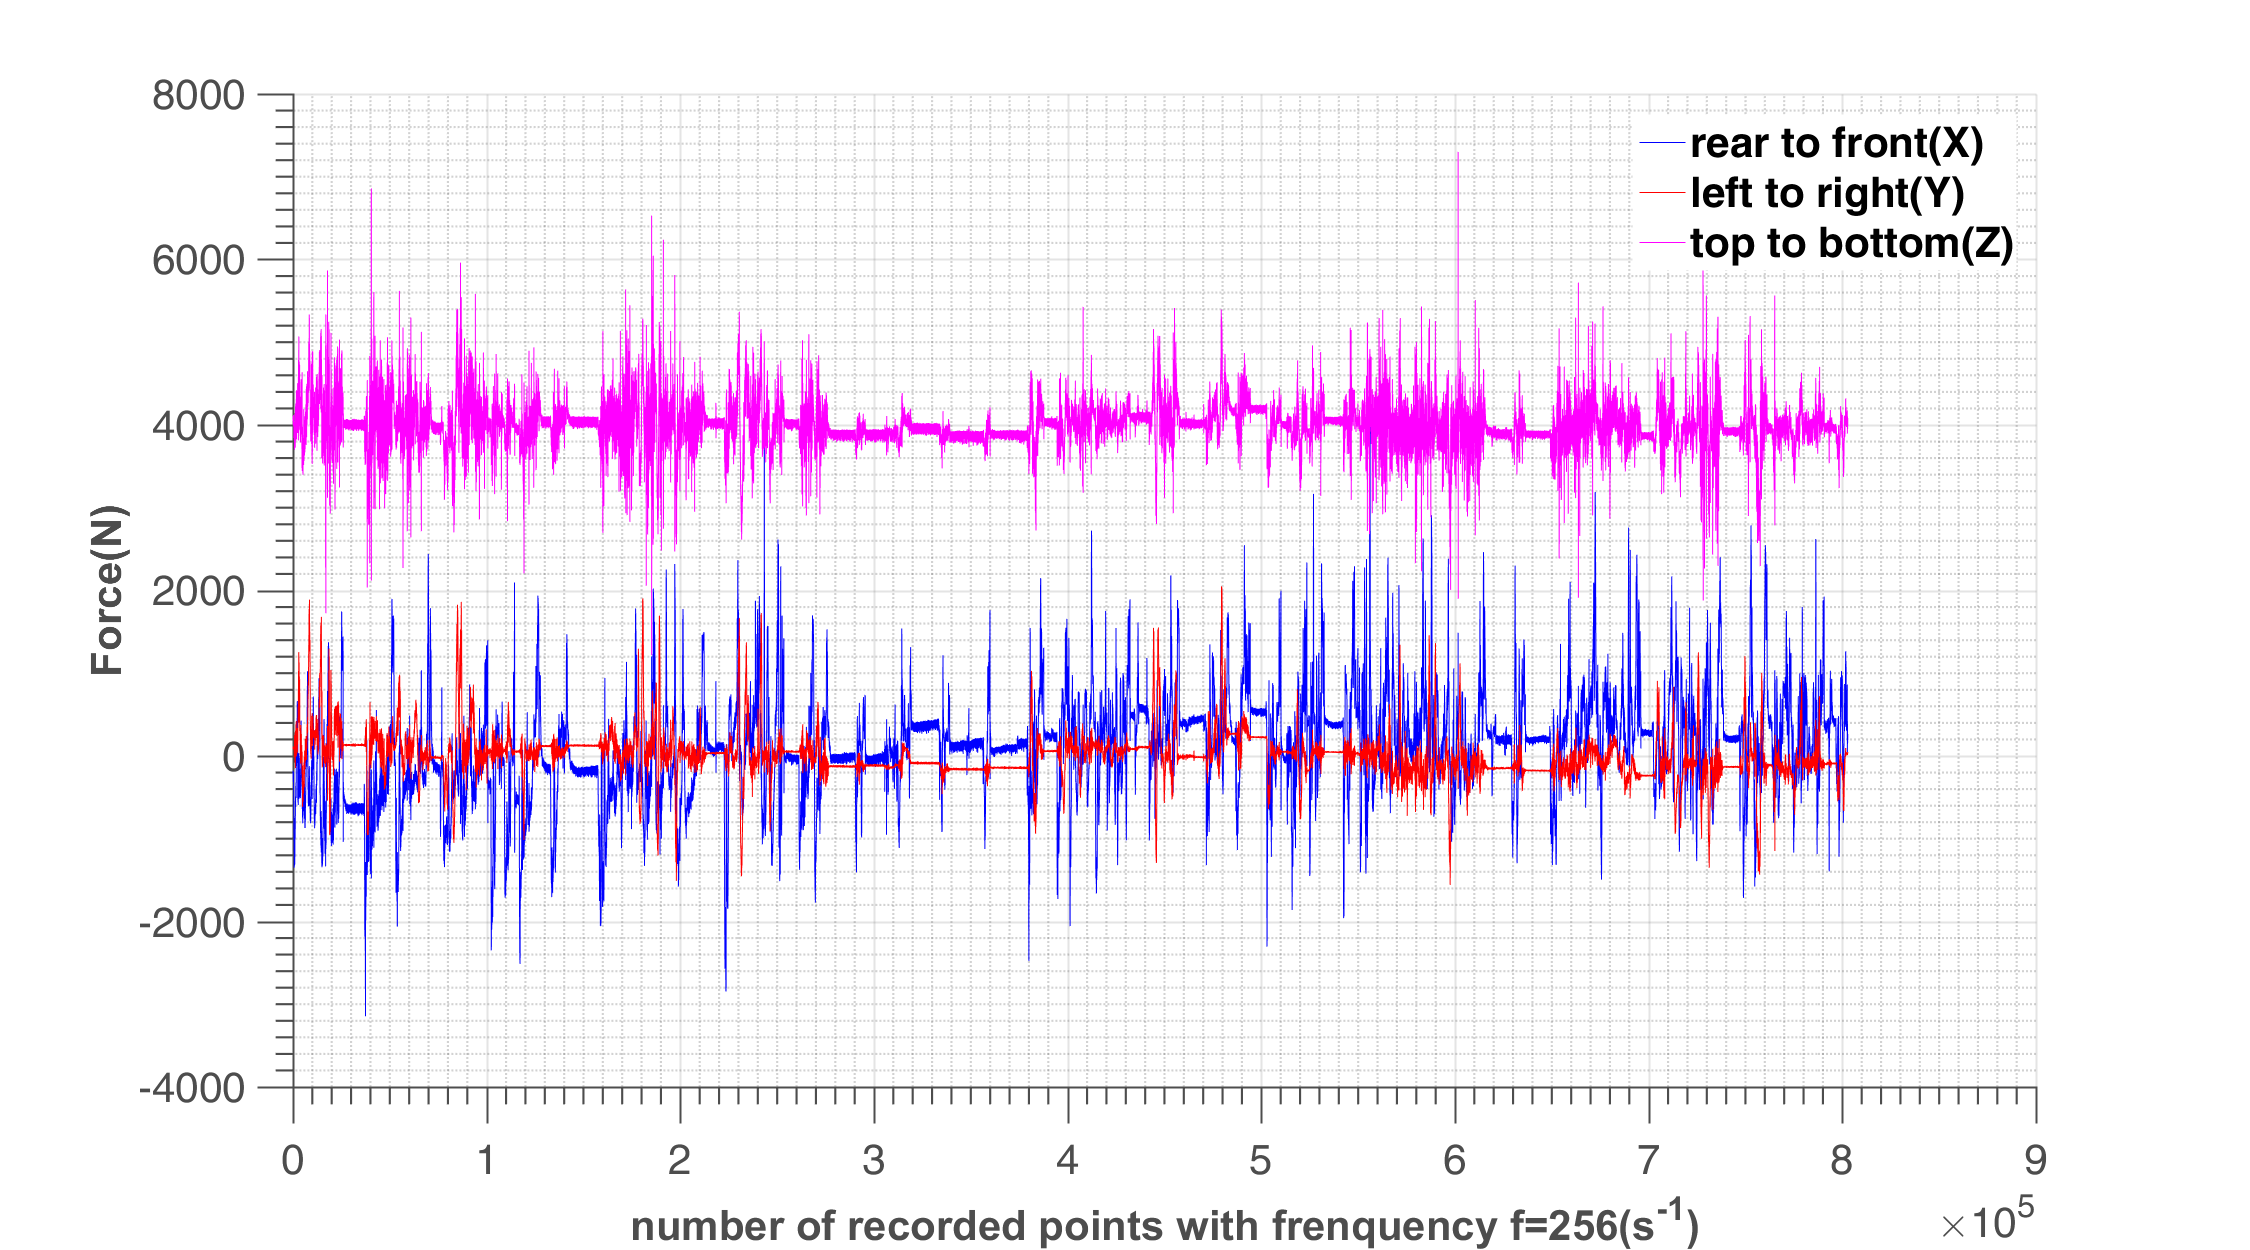
\includegraphics[width=\textwidth]{figures//xyz_suspension.png} 
	\caption{Complex loading of a car suspension arm (data from PSA tests)}
	\label{complexloading}
\end{figure}

As we mentioned before, the mean value of $\alpha$ depends on the loading pattern(sinusoidal, linear division points between max and min stresses in unit cycle,...), but our optimal time step numerical strategy is not loading pattern dependent because it equally divides the range of $\alpha$ during the load history, which means the variation amplitude of stress intensity. So in random loading case with only recorded maximum and minimum load history, we first divide linearly between every 2 recorded points into $100$ time steps, and then perform numerical tests with optimal time step method.

The first tests are performed on aluminum batches, the characteristics of the sample are shown in Tab.\ref{tab:cetim}.
\begin{figure}[!h]
	\centering
	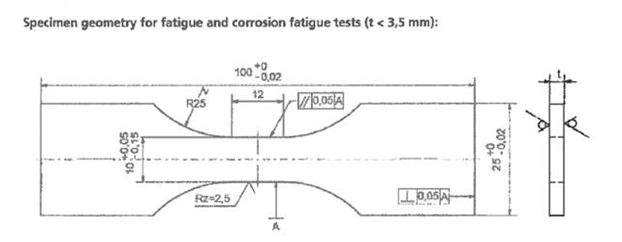
\includegraphics[width=\textwidth]{figures//aluminum_cetim.png} 
	\caption{Specimen geometry for fatigue tests of AW-6106 T6 aluminum(sample given by PSA)}
	\label{fig:aluminum}
\end{figure}
\begin{table}[!h]
	\centering
	\begin{tabular}{ll}
		\hline
		\textbf{Parameters}                                         & \textbf{Value}                    \\ \hline
		Young's modulus                                             & $E=72$ GPa                       \\
		Hardening parameter                                         &  $k=8.5$ MPa \\
		Macroscopic yield stress                                    & $\sigma_y=230$ MPa              \\
		Thickness & $e=2.9mm$                        \\
		Width		 & $l= 9.95mm$                        \\ \hline
	\end{tabular}
	\caption{Material parameters of AW-6106 T6 aluminum}
	\label{tab:cetim}
\end{table}

There are 12 validated uniaxial fatigue tests on the AW-6106 T6 aluminum sample, in which 2 are of constant amplitude load case and 10 involve random  load case. 
The cyclic stress of test number 1(ep01) and test number 2(ep02) are respectively $131.9MPa$ and $97.0MPa$. We first identify the parameters from these two tests. 

\begin{figure}[!h]
	\centering
	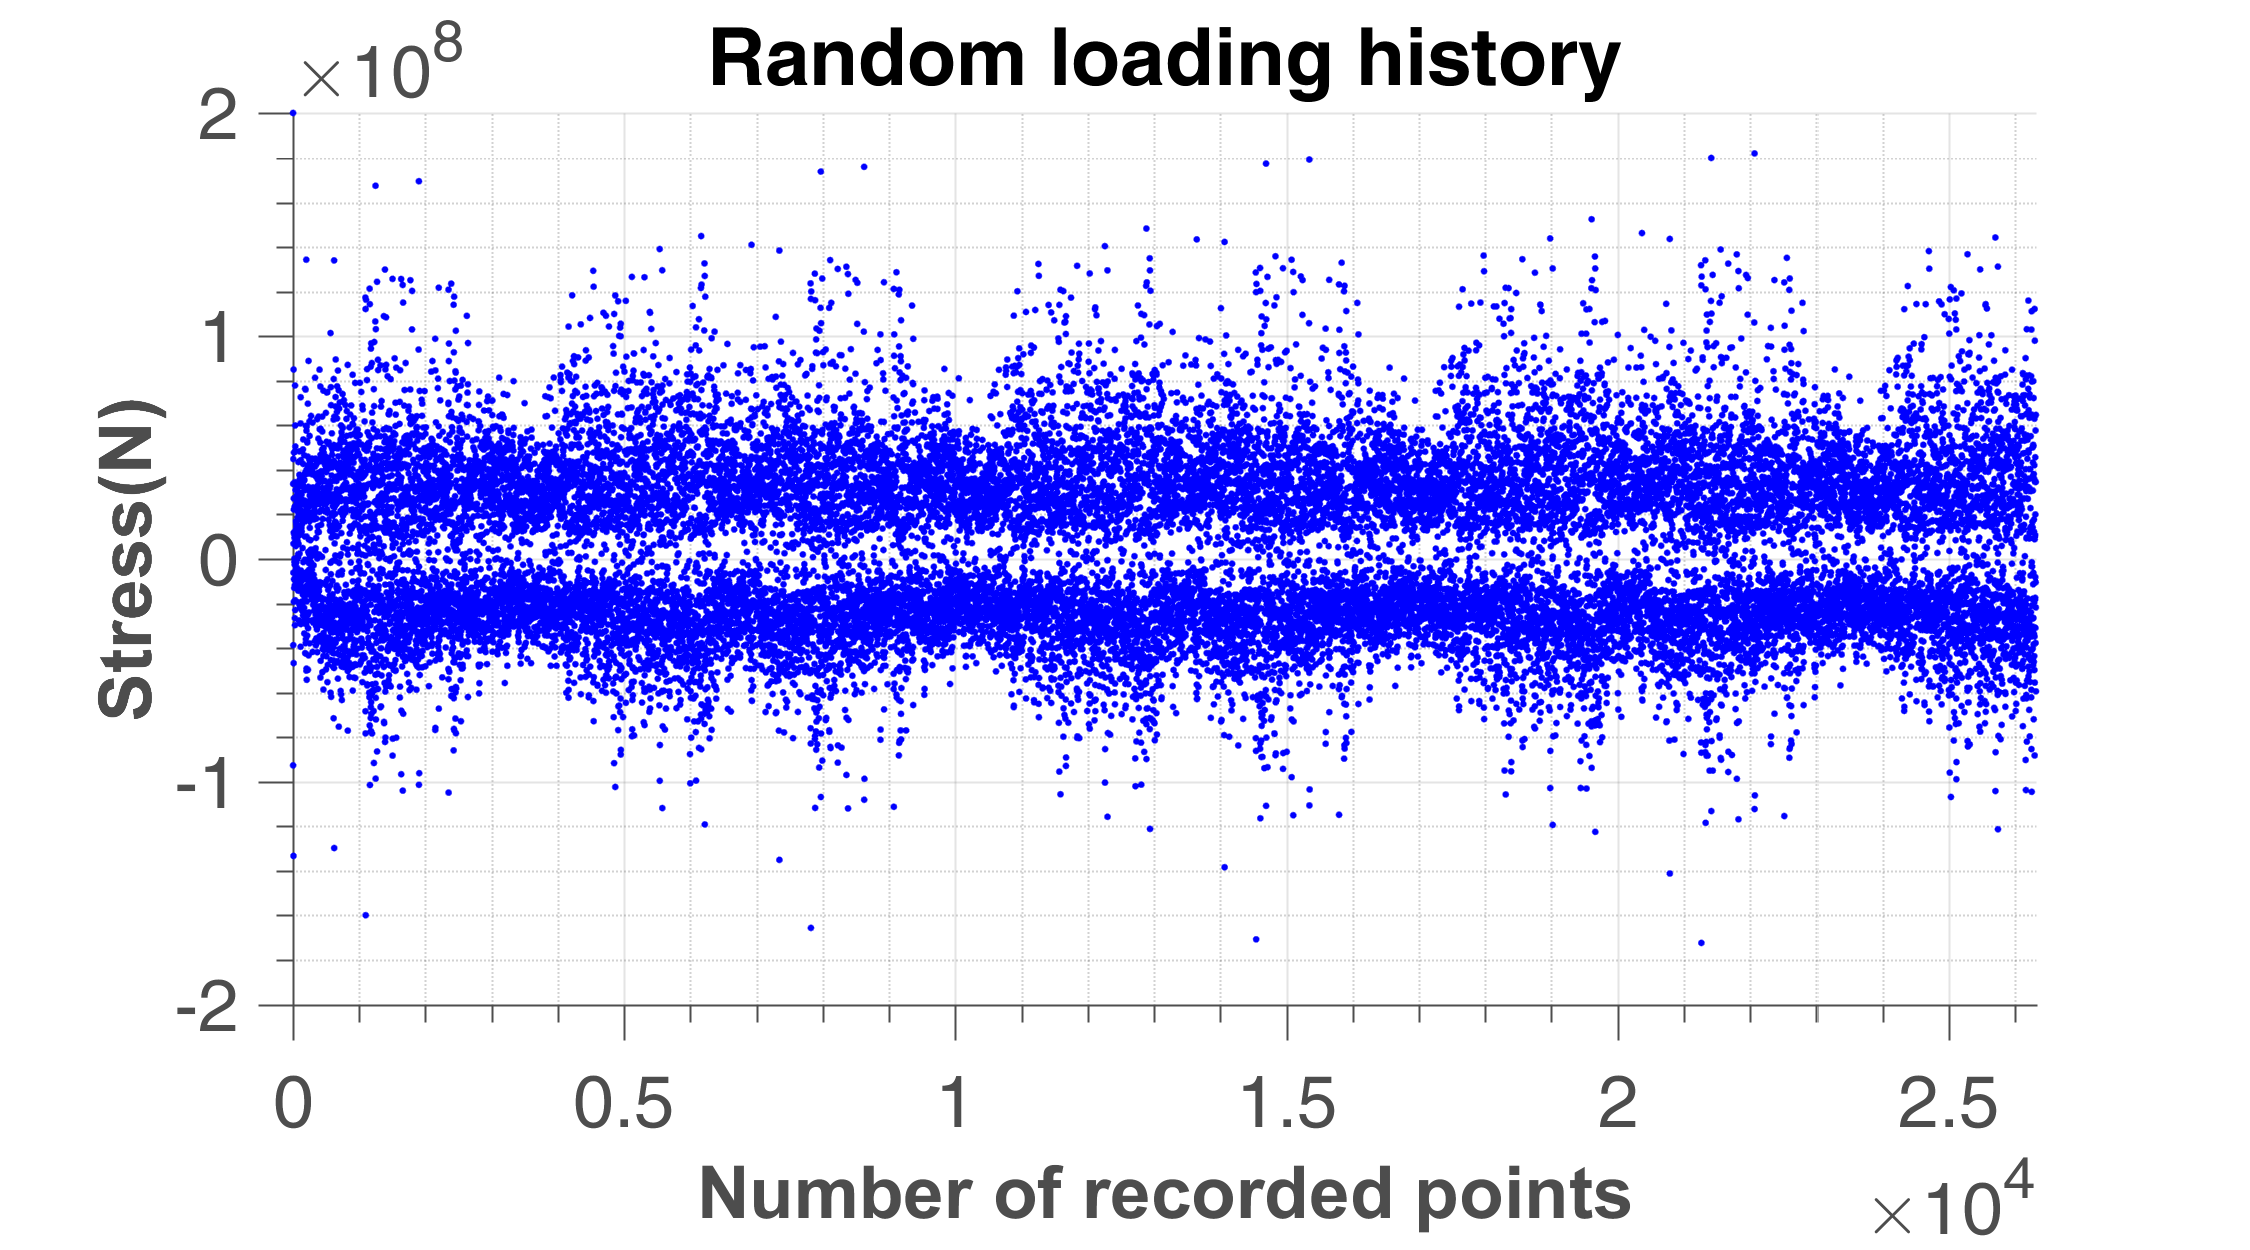
\includegraphics[width=\textwidth]{figures//EP_a_06_random.png} 
	\caption{Random loading history on BATCH\_A\_06 of AW-6106 T6 aluminum (see Tab.\ref{tab:Cetim})}
\end{figure}	
The detailed tests information are shown in Tab.\ref{tab:Cetim}. There are 27000($\pm 2.4\%$) recorded points per repetition. 

\begin{table}[!h]
	\centering
	\begin{tabular}{lllll}
		\hline
		\textbf{Specimen} & \textbf{Fmax (kN)} & \textbf{$\Sigma_{max}$ in the block} & \textbf{Number of repetition} & \textbf{Number of points} \\ \hline
		BATCH\_A\_01      & 3.375              &                                      &                                          & 99892                                \\
		BATCH\_A\_02      & 2.475              &                                      &                                          & 414298                               \\
		BATCH\_A\_04      & nom                & 225.88                               & 95                                       & 2500000                              \\
		BATCH\_A\_05      & nom                & 225.88                               & 156                                      & 4105263                              \\
		BATCH\_A\_06      & nom                & 225.88                               & 145                                      & 3815789                              \\
		BATCH\_A\_07      & nom                & 225.88                               & 90                                       & 2368421                              \\
		BATCH\_A\_08      & nom                & 225.88                               & 194                                      & 5105263                              \\
		BATCH\_A\_09      & nom                & 225.88                               & 197                                      & 5184211                              \\
		BATCH\_A\_10      & nom x 0,9          & 203.292                              & 515                                      & 13552632                             \\
		BATCH\_A\_11      & nom x 0,9          & 203.292                              & 385                                      & 10131579                             \\
		BATCH\_A\_12      & nom x 0,9          & 203.292                              & 424                                      & 11157895                             \\
		BATCH\_A\_13      & nom x 0,9          & 203.292                              & 409                                      & 10763158                             \\ \hline
		BATCH\_B\_01      & nom                & 225.88                               & 121                                      & 3184211                              \\
		BATCH\_B\_02      & nom x 0,8          & 180.704                              & 380                                      & 10000000                             \\
		BATCH\_B\_03      & nom x 0,8          & 180.704                              & 380                                      & 10000000                             \\
		BATCH\_B\_04      & nom x 0,9          & 203.292                              & 406                                      & 10684211                             \\
		BATCH\_B\_05      & nom x 0,9          & 203.292                              & 454                                      & 11947368                             \\
		BATCH\_B\_06      & nom x 0,9          & 203.292                              & 518                                      & 13631579                             \\
		BATCH\_B\_07      & nom x 0,9          & 203.292                              & 553                                      & 14552632                             \\
		BATCH\_B\_08      & nom x 0,9          & 203.292                              & 612                                      & 16105263                             \\
		BATCH\_B\_09      & nom                & 225.88                               & 253                                      & 6657895                              \\
		BATCH\_B\_10      & nom                & 225.88                               & 196                                      & 5157895                              \\
		BATCH\_B\_11      & nom                & 225.88                               & 178                                      & 4684211                              \\
		BATCH\_B\_12      & nom                & 225.88                               & 123                                      & 3236842                              \\ \hline
	\end{tabular}
	\caption{Fatigue tests result on AW-6106 T6 aluminum, test data provided by CETIM}
	\label{tab:Cetim}
\end{table}

We assume the material parameters like Young's modulus $E$, hardening parameter $k$, hydrostatic pressure sensitivity $\lambda_+$(for $\overline{\Sigma}_H=0$ in all cases), macroscopic yield stress $\sigma_y$ and sequence effect sensitivity $a$ are known. We first identify the weakening scales distribution $\beta$, and dissipated energy to failure $W_0$ from cyclic tests ep01 and ep02. Then fit the major damage effect parameter $f$ to see if our assumption is correct or need to be changed. 


The numerical fitting process show that the damage is caused mainly by large stresses (see later). The definition of major stress which affects the value of $\alpha$ now needs to be specified according to the material. To take into account this effect we first find out the proportion stress above a certain value in the repetition signal of random loading, as shown in Tab.\ref{tab.majordamage}.  Here ep\_a and ep\_b are the same material. Since the samples were extracted from aluminum profiles of industrial products,  the two batches correspond to two different times of sampling in the production. The variation is supposed to be representative of the regular tolerances you might have in the production. ep\_a\_01 and ep\_a\_02 are constant amplitude loading which helps identify the power of weakening scale distribution $\beta$. ep\_a\_03 is low cycle fatigue data.  ep\_b\_02 and ep\_b\_03 have infinite life time. The data in the table are grabbed from random signal high cycle fatigue loading history.

\begin{table}[!h]
	\centering
	\begin{tabular}{llllllll}
		\hline
		\textbf{Stress(MPa)\textgreater}  & \textbf{70}    & \textbf{90}    & \textbf{110}   & \textbf{130}    & \textbf{150}    & \textbf{170}    & \textbf{190}    \\
		\textbf{$S_{a}$(MPa)\textgreater} & \textbf{57.15} & \textbf{73.48} & \textbf{89.81} & \textbf{106.14} & \textbf{122.47} & \textbf{138.80} & \textbf{155.13} \\ \hline
		\textbf{ep\_a\_04}           &                & 1.962\%        & 0.904\%        & 0.077\%         & 0.037\%         & 0.018\%         & 0.007\%         \\
		\textbf{ep\_a\_05}           &                & 1.604\%        & 0.784\%        & 0.044\%         & 0.030\%         & 0.007\%         & 0.007\%         \\
		\textbf{ep\_a\_06}           &                & 1.645\%        & 0.784\%        & 0.045\%         & 0.030\%         & 0.007\%         & 0.007\%         \\
		\textbf{ep\_a\_07}           &                & 1.632\%        & 0.788\%        & 0.048\%         & 0.029\%         & 0.007\%         & 0.007\%         \\
		\textbf{ep\_a\_08}           &                & 1.644\%        & 0.787\%        & 0.048\%         & 0.037\%         & 0.007\%         & 0.007\%         \\
		\textbf{ep\_a\_09}           &                & 1.655\%        & 0.800\%        & 0.048\%         & 0.037\%         & 0.007\%         & 0.007\%         \\
		\textbf{ep\_a\_10}           &                & 0.768\%        & 0.134\%        & 0.007\%         & 0.000\%         & 0.000\%         & 0.000\%         \\
		\textbf{ep\_a\_11}           &                & 0.772\%        & 0.145\%        & 0.007\%         & 0.000\%         & 0.000\%         & 0.000\%         \\
		\textbf{ep\_a\_12}           &                & 0.779\%        & 0.133\%        & 0.011\%         & 0.000\%         & 0.000\%         & 0.000\%         \\
		\textbf{ep\_a\_13}           &                & 0.775\%        & 0.141\%        & 0.007\%         & 0.000\%         & 0.000\%         & 0.000\%         \\ \hline
		\textbf{ep\_b\_01}           & 4.739\%        & 1.737\%        & 0.840\%        & 0.224\%         & 0.049\%         & 0.034\%         & 0.004\%         \\
		\textbf{ep\_b\_04}           & 1.999\%        & 0.745\%        & 0.156\%        & 0.034\%         & 0.004\%         & 0.000\%         & 0.000\%         \\
		\textbf{ep\_b\_05}           & 2.010\%        & 0.749\%        & 0.148\%        & 0.034\%         & 0.008\%         & 0.000\%         & 0.000\%         \\
		\textbf{ep\_b\_06}           & 1.999\%        & 0.790\%        & 0.118\%        & 0.034\%         & 0.008\%         & 0.000\%         & 0.000\%         \\
		\textbf{ep\_b\_07}           & 2.029\%        & 0.756\%        & 0.152\%        & 0.034\%         & 0.008\%         & 0.000\%         & 0.000\%         \\
		\textbf{ep\_b\_08}           & 1.999\%        & 0.737\%        & 0.137\%        & 0.034\%         & 0.008\%         & 0.000\%         & 0.000\%         \\
		\textbf{ep\_b\_09}           & 4.663\%        & 1.687\%        & 0.798\%        & 0.205\%         & 0.049\%         & 0.034\%         & 0.004\%         \\
		\textbf{ep\_b\_10}           & 4.712\%        & 1.744\%        & 0.809\%        & 0.224\%         & 0.046\%         & 0.034\%         & 0.004\%         \\
		\textbf{ep\_b\_11}           & 4.636\%        & 1.664\%        & 0.790\%        & 0.209\%         & 0.049\%         & 0.034\%         & 0.004\%         \\
		\textbf{ep\_b\_12}           & 0.775\%        & 0.141\%        & 0.007\%        & 0.000\%         & 0.000\%         & 0.000\%         & 0.000\%         \\ \hline
	\end{tabular}
	\caption{Proportion of stress(MPa) above different threshold with $\Sigma_y$=230MPa, test data provided by CETIM on AW-6106 T6 aluminum.}
	\label{tab.majordamage}
\end{table}

\begin{table}[!h]
	\centering
	\begin{tabular}{lrrrrrrr}
		\hline
		\multicolumn{8}{c}{\textbf{Random amplitude sensitivity test with $f(\beta)=\beta$}}                                                                                                                                                                                                                                             \\ \hline
		& \multicolumn{1}{r}{\textbf{Ref}} & \multicolumn{1}{r}{\textbf{Min}} & \multicolumn{1}{r}{\textbf{Max}} & \multicolumn{1}{r}{\textbf{Ref\_n}} & \multicolumn{1}{r}{\textbf{Min\_n}} & \multicolumn{1}{r}{\textbf{Max\_n}} & \multicolumn{1}{r}{\textbf{Sensitivity}} \\ \hline
		\textbf{$\beta$}   & 1.1                                          & 1.05                             & 1.50                             & 4220452                                    & 7469257                             & 1799585                             & -3.28 
		\\
		\textbf{$\lambda$} & 0.1                                          & 0.05                             & 0.50                             & 4220452                                   & 4566335                             & 2175991                             & -0.13                                    \\
		\textbf{$W_0$}     & 3.27e8                                     & 1.00e8                         & 5.00e8                         & 4220452                                    & 1321761                             & 6420810                             & 0.99                                    \\
		\textbf{$a$}       & 0.1                                          & 0.05                             & 0.15                             & 4220452                                   & 7156622                             & 2827894                             & -1.03                                   \\ \hline
	\end{tabular}
	\caption{Parameters sensitivity at random loading of ep05 on AW-6106 T6 aluminum}
	\label{tab.sensitivity_random1}
\end{table}

From Tab.\ref{tab.sensitivity_const2} and Tab.\ref{tab.sensitivity_random2} we can see $f$ has positive correlation with $\beta$ in high cycle fatigue which is the regime we focus on.  However, very large value of $f$ may ignore the small stress variations in the loading history, which goes against our assumption that small stresses also contribute to material damage. So we give $f=1.1$ in high cycle random loading case to minimize the relative error.
\begin{table}[!h]
	\centering
	\begin{tabular}{lrrrrrrr}
		\hline
		\multicolumn{8}{c}{\textbf{Constant amplitude sensitivity test with $f(\beta)\neq\beta$}}                                                                                                                                                                                                 \\ \hline
		& \multicolumn{1}{l}{\textbf{Ref}} & \multicolumn{1}{l}{\textbf{Min}} & \multicolumn{1}{l}{\textbf{Max}} & \multicolumn{1}{l}{\textbf{Ref\_n}} & \multicolumn{1}{l}{\textbf{Min\_n}} & \multicolumn{1}{l}{\textbf{Max\_n}} & \multicolumn{1}{l}{\textbf{Sensitivity}} \\ \hline
		\textbf{$\beta$}    & 1.1                              & 1.05                             & 1.50                             & 414233                              & 797377                              & 213682                              & -3.44                                    \\
		\textbf{$\lambda$}  & 0.1                              & 0.05                             & 0.50                             & 414233                              & 449598                              & 443376                              & 0.00                                     \\
		\textbf{$W_0$}      & 3.27e8                         & 1.00e8                         & 5.00e8                         & 414233                              & 137498                              & 687209                              & 1.08                                     \\
		\textbf{$a$}        & 0.1                              & 0.05                             & 0.15                             & 414233                              & 672869                              & 324754                              & -0.84                                    \\
		\textbf{$f(\beta)$} & 1.1                              & 1.05                             & 1.5                              & 414233                              & 441661          &511644          & 0.41                                     \\ \hline
	\end{tabular}
	\caption{Parameters sensitivity at cyclic loading of ep02 on AW-6106 T6 aluminum}
	\label{tab.sensitivity_const2}
\end{table}
\begin{table}[!h]
	\centering
	\begin{tabular}{lrrrrrrr}
		\hline
		\multicolumn{8}{c}{\textbf{Random amplitude sensitivity test with $f(\beta)\neq\beta$}}                                                                                                                                                                                                   \\ \hline
		\textbf{}           & \multicolumn{1}{l}{\textbf{Ref}} & \multicolumn{1}{l}{\textbf{Min}} & \multicolumn{1}{l}{\textbf{Max}} & \multicolumn{1}{l}{\textbf{Ref\_n}} & \multicolumn{1}{l}{\textbf{Min\_n}} & \multicolumn{1}{l}{\textbf{Max\_n}} & \multicolumn{1}{l}{\textbf{Sensitivity}} \\ \hline
		\textbf{$\beta$}    & 1.1                              & 1.05                             & 1.50                             & 4220452                             & 7254554                             & 2472791                             & -2.77                                    \\
		\textbf{$\lambda$}  & 0.1                              & 0.05                             & 0.50                             & 4220452                             & 4566335                             & 2175991                             & -0.13                                    \\
		\textbf{$W_0$}      & 3.27e8                         & 1.00e8                         & 5.00e8                         & 4220452                             & 1321761                             & 6420810                             & 0.99                                     \\
		\textbf{$a$}        & 0.1                              & 0.05                             & 0.15                             & 4220452                             & 7156622                             & 2827894                             & -1.03                                    \\
		\textbf{$f(\beta)$} & 1.1                              & 1.05                             & 1.5                              & 4220452                             & 4341560                             & 3052299                             & -0.75                                    \\ \hline
	\end{tabular}
	\caption{Parameters sensitivity at random loading of ep05 on AW-6106 T6 aluminum}
	\label{tab.sensitivity_random2}
\end{table}
The sensitivity of parameters is calculated by dividing the percentage of variation of  number of points to failure with respect to the reference number of points to failure, by the percentage of variation of parameter with respect to the reference parameter, as shown in Eq.\eqref{eq.sensitivity}.
\begin{equation}
sensitivity = \dfrac{\left( Max_n-Min_n\right)/Ref_n}{\left( Max-Min\right)/Ref}.
\label{eq.sensitivity}
\end{equation}



%The standard S-N curve is fitted with fatigue data provided by Cetim(the red line). Analytical calculation of mean dissipated energy and of the average value of $\alpha$ on one cycle, and  integration of the differential equation in D with these mean values is provided. The comparison with numerical method where we have changing $\alpha$ and $W$ at each time step in standard $S-N$ curve is shown in \figref{fig.para}:a. This analytical strategy is proposed to give a much cheaper way to treat cyclic loadings for high cycle fatigue. However, we find that there is a constant relative error between the analytical result and numerical one and the analytical one is more conservative. The relative error is due to integration of damage $D$ from Eq.\eqref{eq.DWcyc} to Eq.\eqref{eq.NFWcyc}. We assumed $\alpha$ is constant during damage accumulation which in step by step method is not the case.

%The influence of all the parameters on constant amplitude cyclic load using Eq.\eqref{eq.nf}  are shown in \figref{fig.para}.
%\begin{Figure}[!h]{The influence of parameters on the shape and limit of S-N curve}[fig.para]
%	\graphfile*[42]{figures//SNnumerical.png}[S-N curve using numerical and analytical method]
%	\graphfile*[42]{figures//SNlam.png}[The $\lambda$ influence on S-N curve]
%	\\
%    \graphfile*[42]{figures//SNa.png}[The $a$ influence on S-N curve]
%	\graphfile*[42]{figures//SNWF.png}[The $W_F$ influence on S-N curve]
%	\\
%	\graphfile*[42]{figures//SNb.png}[The $\beta$ influence on S-N curve]
%	\graphfile*[42]{figures//SNpb.png}[The $f(\beta)$ influence on S-N curve]
%\end{Figure}
%The different parameters impacts are shown in purple curves. We can see the weakening scale $\beta$ changes the inclination of S-N curve. $\beta$ is also the magnification factor which magnify large stress damage as well as minify small stress damage.  Not surprisingly the hydrostatic stress sensitivity $\lambda$ has more influence on large stress. The amplification factor of load intensity in damage accumulation $a$ and  energy scaling in damage accumulation law $W_0$ adapts to fatigue life without changing the shape the S-N curve.

After the fitting process, the reference parameters value we use are in Tab.\ref{tab.cetim.alp}.
\begin{table}[!h]
	\centering
	\begin{tabular}{lrrrrr}
		\hline
		\textbf{Constant $\alpha$} & \textbf{$W_0$(MPa)} & \textbf{$\lambda_+=\lambda_-$} & \textbf{$\beta$}  & \textbf{$\alpha$}& \textbf{$f$}\\
		& 326.9         & 0.1               & 1.1            & 0.7      & 1.1                    \\ \hline
		\textbf{Changing $\alpha$} & \textbf{$W_0$(MPa)} & \textbf{$\lambda_+=\lambda_-$} & \textbf{$\beta$}  & \textbf{$a$} & \textbf{$f$}\\
		& 326.9         & 0.1               & 1.1            & 0.1         & 1.1                \\ \hline
	\end{tabular}
	\caption{The parameters in 1D cyclic and random loading on AW-6106 T6
		aluminum fatigue tests by Cetim}
	\label{tab.cetim.alp}
\end{table}

The best fitted results with constant $\alpha$ are shown in \figref{fig.Cetimerralpfix}. The dispersion is relatively large. In conclusion, we are not able to predict the random stress amplitude fatigue life with fixed $\alpha$, because random stresses not only cause different energy dissipations, but also show a distinctive load sequence effect. So we have to update the value of $\alpha$ at each time step. 

\begin{figure}[!h]
	\centering
	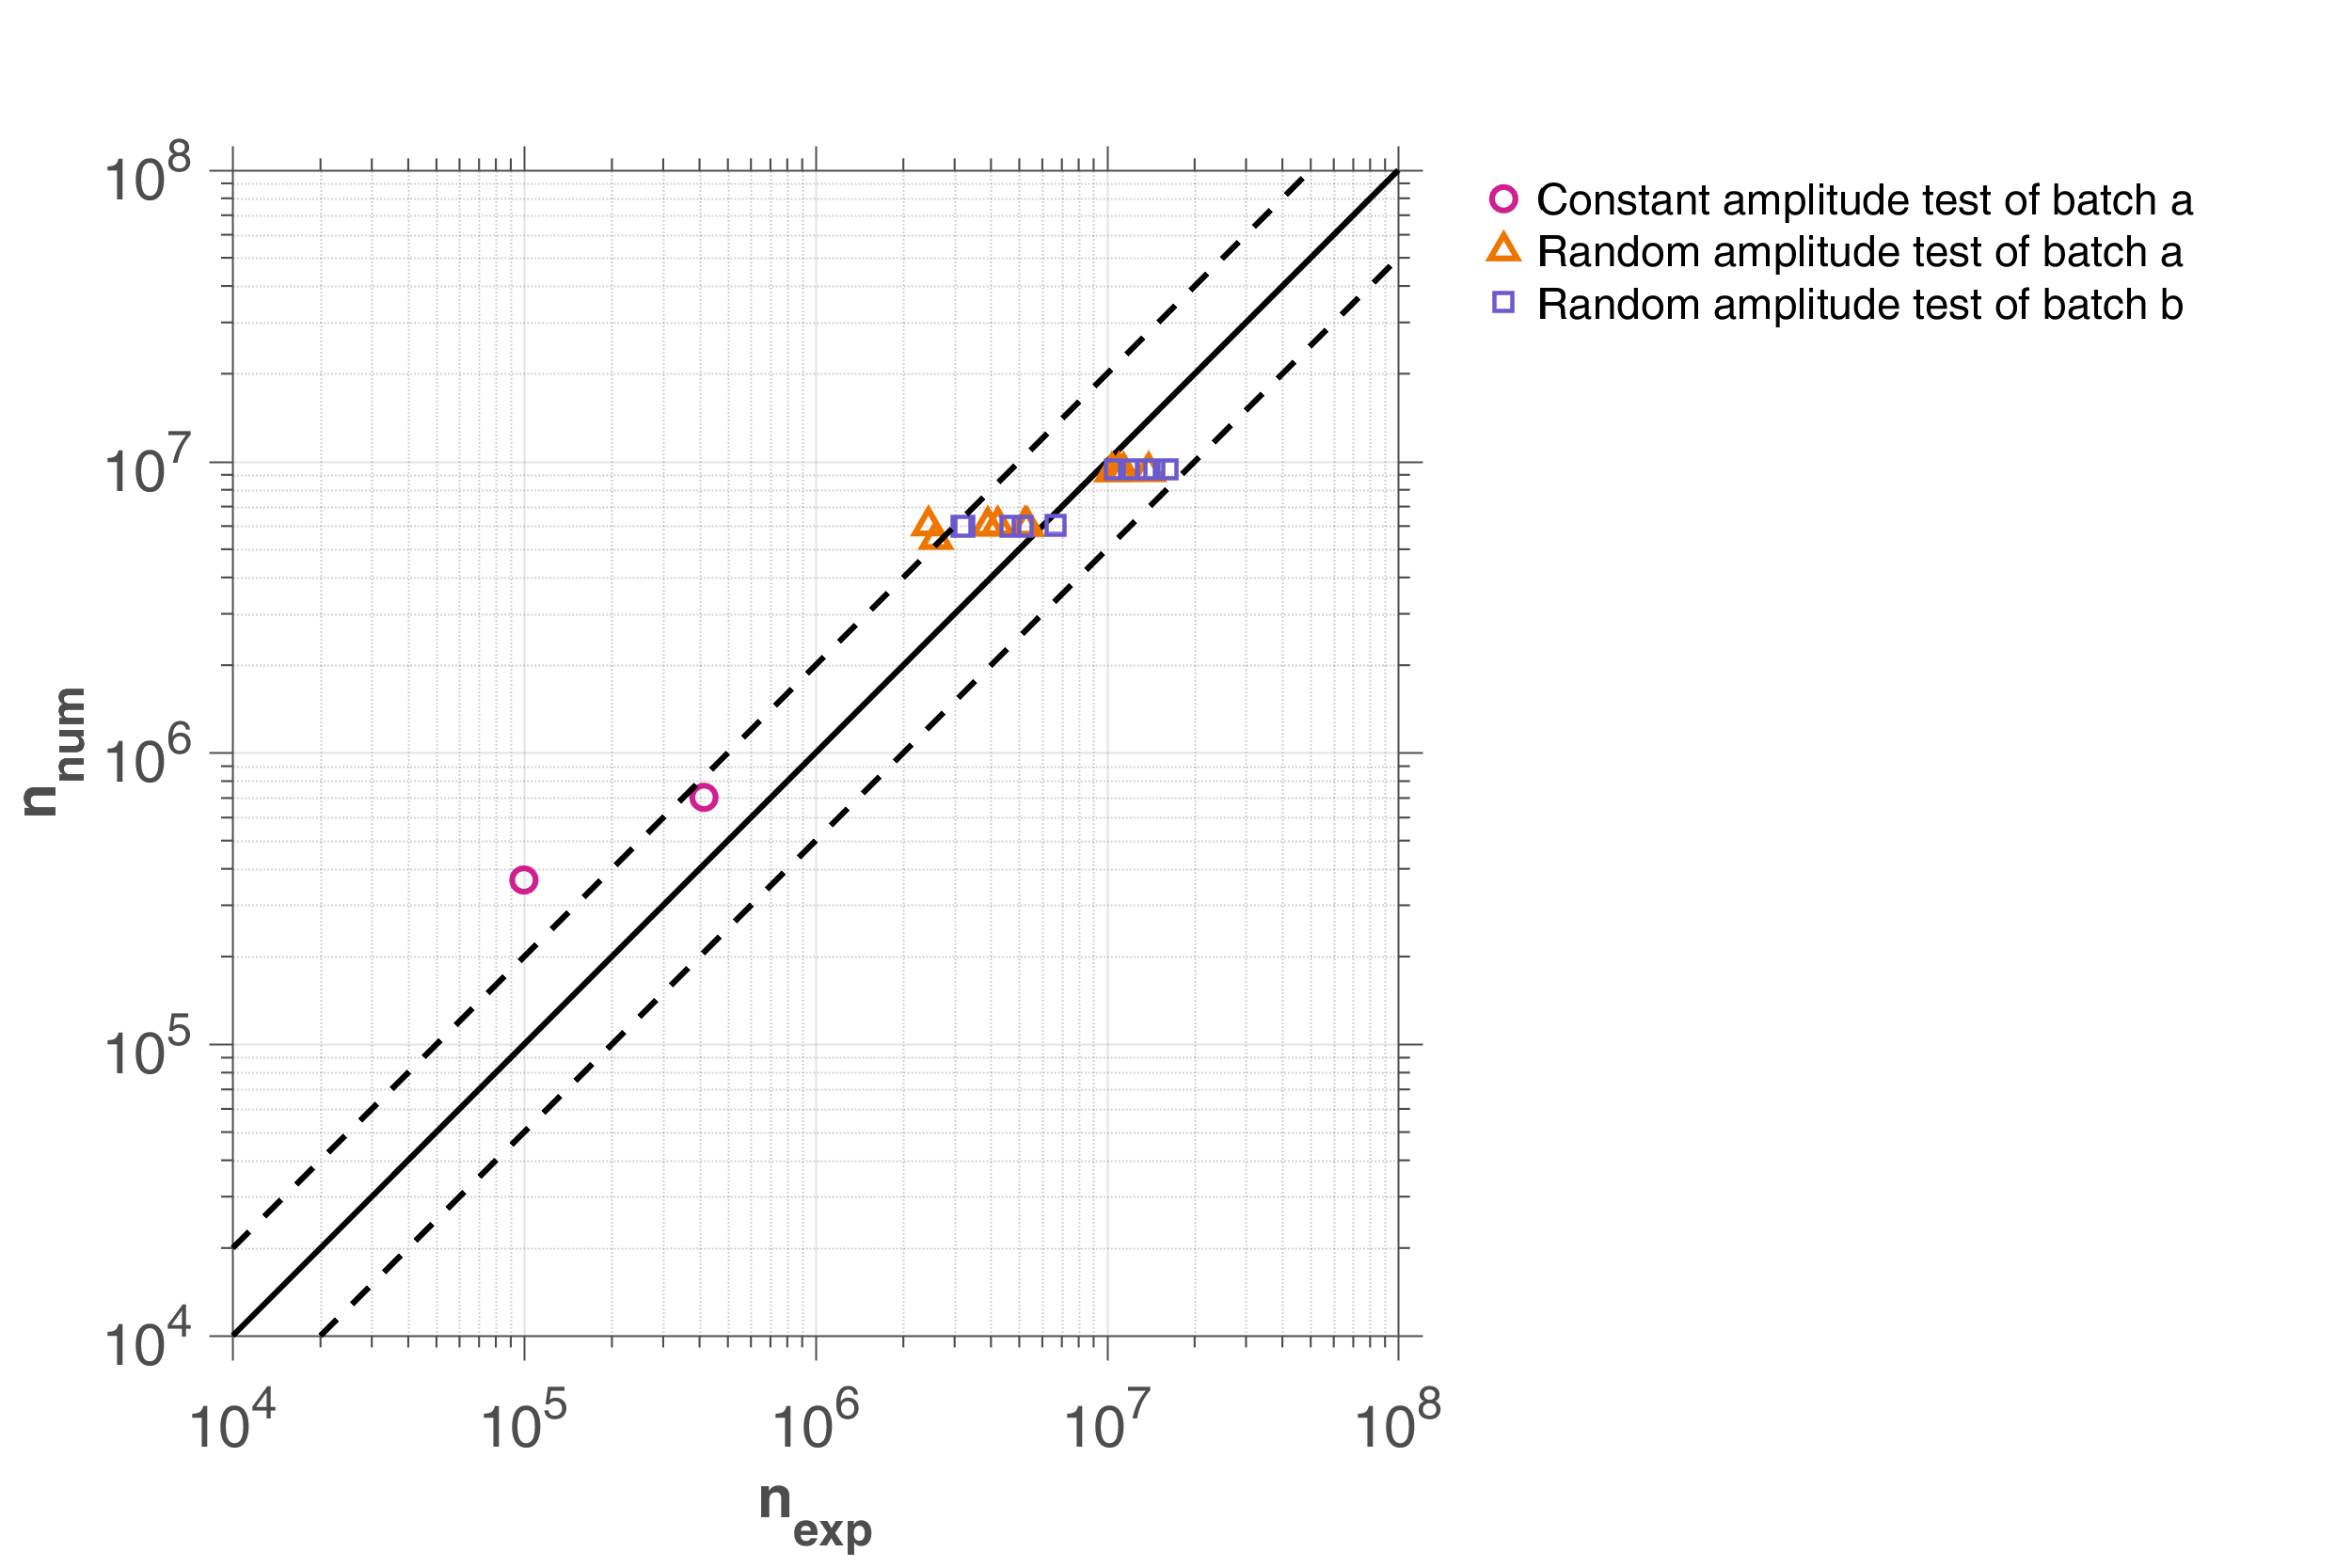
\includegraphics[width=\textwidth]{figures//Cetim_err_alpfix.png} 
	\caption{Comparison between experimental and numerical results of 1D cyclic and random loading on aluminum fatigue tests by CETIM with constant $\alpha$ from the first row of Tab.\ref{tab.cetim.alp}}
	\label{fig.Cetimerralpfix}
\end{figure}

We can find that the numerical results are satisfactory when we introduce a major damage influence through the construction of a load dependent $\alpha$. The dispersion figure with distinction of major damage is depicted in \figref{fig.Cetimerr}. Here it is necessary to control the parameter $a$ to make sure $\alpha>0$ in the most severe situation.

\begin{figure}[!h]
	\centering
	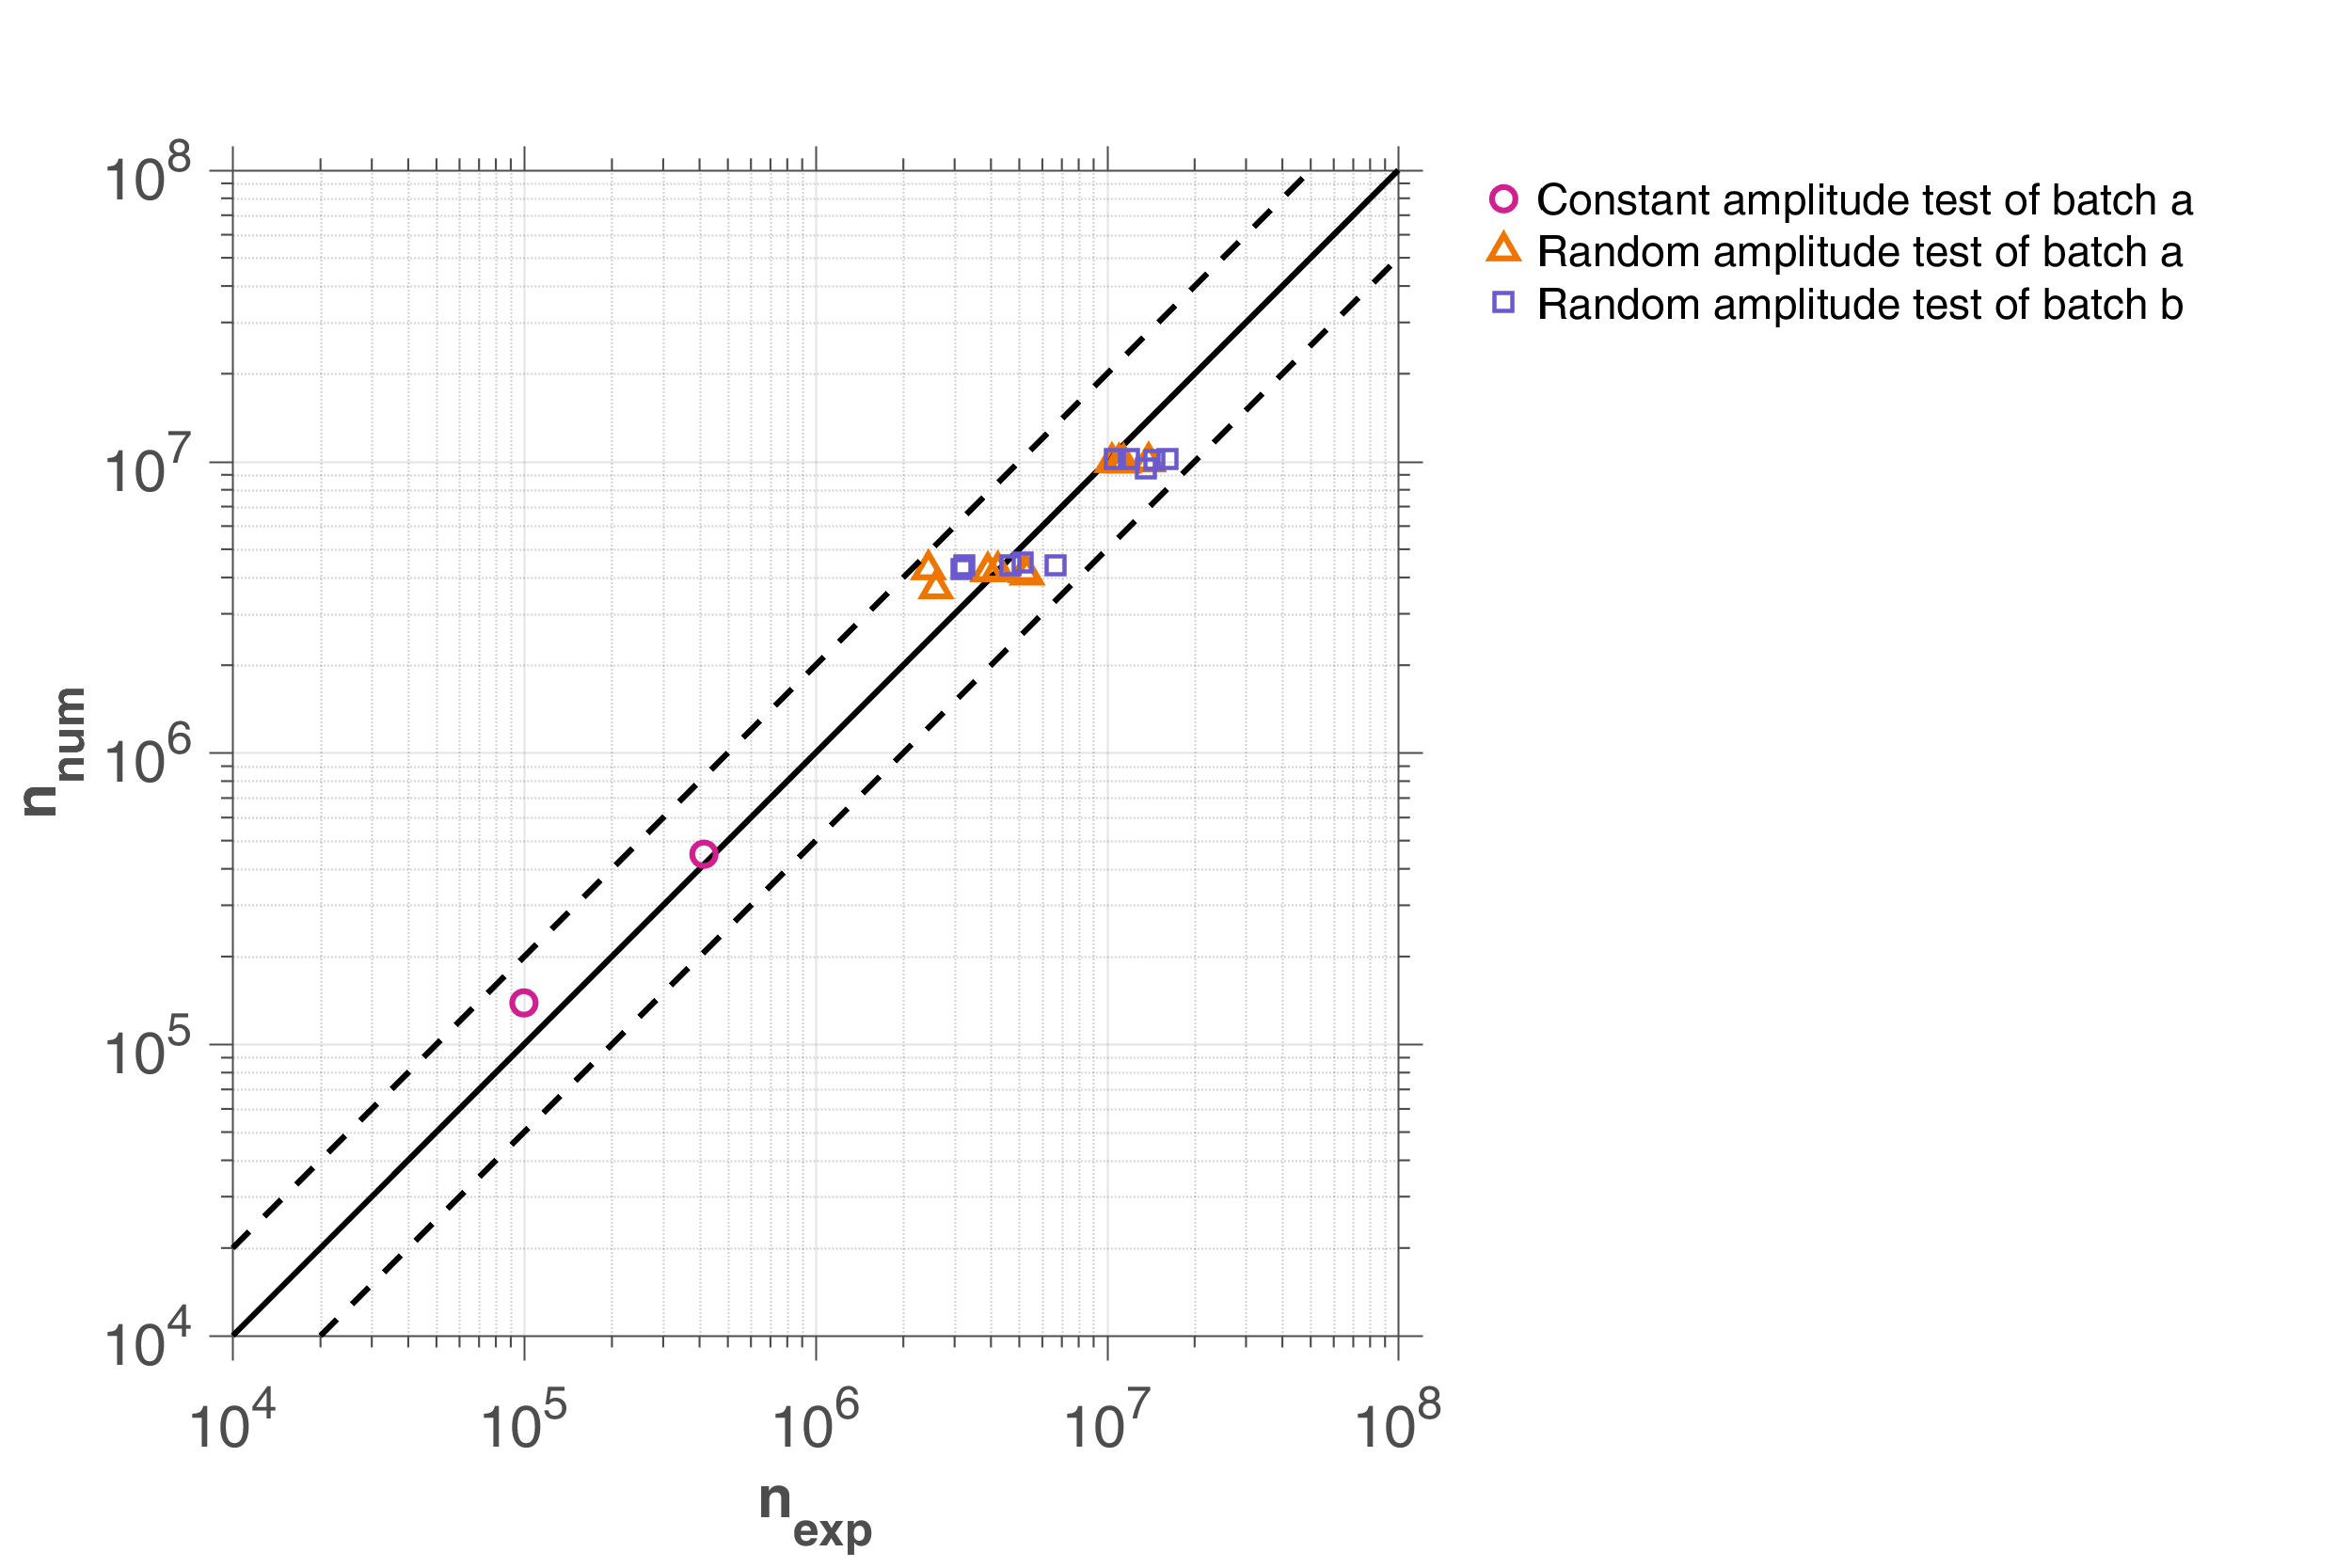
\includegraphics[width=\textwidth]{figures//Cetim_err.png} 
	\caption{Comparison between experimental and numerical results of 1D cyclic and random loading on aluminum fatigue tests by Cetim with load dependent $\alpha$. Coefficients data are given in the second row of Tab.\ref{tab.cetim.alp}}
	\label{fig.Cetimerr}
\end{figure}

\clearpage
\section{Experimental validation of the model on aluminum 6082 T6}
\subsection{Presentation of aluminum 6082 T6}

The material tested is aluminum 6082 T6, used by \cite{susmel2003multiaxial} to validate their method of lifetime prediction. The mechanical properties of this material are summarized in Tab.\ref{tab.al6082t6}.

\begin{table}[!h]
	\centering
	\begin{tabular}{|c|c|c|c|}
		\hline
		\textbf{$E${[}GPa{]}} & \textbf{$\sigma_{y}${[}MPa{]}} & \textbf{$\sigma_u${[}MPa{]}} & \textbf{$\nu$} \\ \hline
		69.4                                  & 298                                & 343                         & 0.33                 \\ \hline
	\end{tabular}
	\caption{Mechanical and dynamic characteristics of aluminum 6082 T6 (\cite{susmel2003multiaxial})}
	\label{tab.al6082t6}
\end{table}

\vspace{6pt}
\textbf{Specimens of aluminum 6082 T6}
\vspace{6pt}

The specimens were made from the drawn bars (diameter 30 mm) and the geometrical shape of which is given in \figref{fig:aluminum6082T6}. They are successively polished with $6-\mu m$ diamond compounds until a good mirror-like finish is obtained.
\begin{figure}[!h]
	\centering
	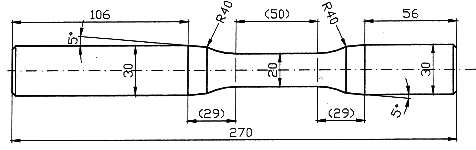
\includegraphics[width=0.7\textwidth]{figures//aluminum6082T6sample.png} 
	\caption{Specimen geometry for fatigue tests of aluminum 6082 T6 (dimension in millimeters)\ref{susmel2003multiaxial}}
	\label{fig:aluminum6082T6}
\end{figure}

\subsection{Fatigue tests on aluminum 6082 T6}
The simulated tests are purely alternate and summarized in Tables \ref{tab.AL6082T6BT1D} and \ref{tab.AL6082T6BT2D}. They consist of simple tests in bending, torsion and bending-torsion in phase and out-phase for two cases of biaxial stress ratio, $\lambda=\tau_{xy,a}/\sigma_{x,a}$
($\lambda>1$ and $\lambda<1$). The expected lifetimes range from $10^4$ to $1.5\times10^6$ cycles. 
\begin{table}[!h]
	\centering
	\begin{tabular}{|l|l|l|l|l|l|}
		\hline
		Batch $N^\circ$ & $\sigma_{x,a}${[}MPa{]} & $\tau_{xy,a}${[}MPa{]} & $\lambda$ & $\delta [^\circ]$ & $N_{f,5\%}${[}Cycles{]} \\ \hline
		P1B1 & 190 & 0 & 0 & 0 & 160000 \\ \hline
		P2B2 & 180 & 0 & 0 & 0 & 248518 \\ \hline
		P3B3 & 164 & 0 & 0 & 0 & 444411 \\ \hline
		P4B4 & 144 & 0 & 0 & 0 & 1069220 \\ \hline
		P5B5 & 224 & 0 & 0 & 0 & 56285 \\ \hline
		P6B4 & 145 & 0 & 0 & 0 & 1238325 \\ \hline
		P7B1 & 187 & 0 & 0 & 0 & 200480 \\ \hline
		P8B3 & 161 & 0 & 0 & 0 & 423590 \\ \hline
		PC9T1 & 0 & 117 & $\infty$ & 0 & 534032 \\ \hline
		PC10T2 & 0 & 155 & $\infty$ & 0 & 26987 \\ \hline
		PC11T3 & 0 & 127 & $\infty$ & 0 & 76665 \\ \hline
		PC12T3 & 0 & 127 & $\infty$ & 0 & 132295 \\ \hline
		PC13T1 & 0 & 117 & $\infty$ & 0 & 203535 \\ \hline
		PC14T2 & 0 & 155 & $\infty$ & 0 & 16195 \\ \hline
		PC15T4 & 0 & 106 & $\infty$ & 0 & \textgreater1.1E6 \\ \hline
		PC16T4 & 0 & 104 & $\infty$ & 0 & 565150 \\ \hline
	\end{tabular}
	\caption{Simple bending and torsion tests (R = -1), data from \cite{susmel2003multiaxial}}
	\label{tab.AL6082T6BT1D}
\end{table}
\begin{table}[!h]
	\centering
	\begin{tabular}{|l|l|l|l|l|l|}
		\hline
		Batch $N^\circ$ & $\sigma_{x,a}${[}MPa{]} & $\tau_{xy,a}${[}MPa{]} & $\lambda$ & $\delta [^\circ]$ & $N_{f,5\%}${[}Cycles{]} \\ \hline
		P17BT1 & 57 & 100 & 1.75 & 0 & 266435 \\ \hline
		P18BT2 & 51 & 84 & 1.65 & 0 & 1119254 \\ \hline
		P19BT2 & 51 & 84 & 1.65 & 0 & 1416225 \\ \hline
		P20BT3 & 71 & 118 & 1.66 & 0 & 83000 \\ \hline
		P21BT3 & 70 & 118 & 1.69 & 0 & 75695 \\ \hline
		P22BT1 & 59 & 99 & 1.68 & 0 & 630325 \\ \hline
		P23BT4 & 132 & 97 & 0.73 & 0 & 157210 \\ \hline
		P24BT4 & 132 & 99 & 0.75 & 0 & 126470 \\ \hline
		P25BT5 & 144 & 107 & 0.74 & 0 & 35450 \\ \hline
		P26BT5 & 149 & 105 & 0.7 & 0 & 68465 \\ \hline
		P27BT6 & 122 & 90 & 0.74 & 0 & 252658 \\ \hline
		P28BT7 & 116 & 83 & 0.72 & 0 & 316149 \\ \hline
		P30BT8 & 148 & 66 & 0.45 & 90 & 278836 \\ \hline
		P31BT9 & 152 & 47 & 0.31 & 90 & 465010 \\ \hline
		P32BT8 & 149 & 68 & 0.46 & 90 & 118965 \\ \hline
		P33BT9 & 155 & 72 & 0.46 & 90 & 447525 \\ \hline
		P34BT10 & 190 & 105 & 0.55 & 90 & 47940 \\ \hline
		P35BT10 & 189 & 106 & 0.56 & 90 & 30995 \\ \hline
		P36BT11 & 79 & 129 & 1.63 & 90 & 23080 \\ \hline
		P37BT12 & 69 & 110 & 1.59 & 90 & 202807 \\ \hline
		P38BT13 & 68 & 99 & 1.46 & 90 & 262980 \\ \hline
		P39BT13 & 68 & 99 & 1.46 & 90 & 398615 \\ \hline
		P41BT15 & 79 & 116 & 1.47 & 90 & 46045 \\ \hline
	\end{tabular}
	\caption{In-phase and out-of-phase bending-torsion tests (R = -1), data from \cite{susmel2003multiaxial}}
	\label{tab.AL6082T6BT2D}
\end{table}

In the Tables \ref{tab.AL6082T6BT1D} and \ref{tab.AL6082T6BT2D}, $\sigma_{x,a}$ is the normal stress amplitude, $\tau_{xy,a}$ is the torsion amplitude, $\lambda$ is the biaxial stress ratio, $\delta$ is the phase shift between the components of applied stresses and $N_{f,5\%}$ represents the number of cycles at break, defined by a 5\% decrease in flexural or torsional stiffness.

It is interesting to note that a reduced amount of plasticity was measured by strain gauges in the PC10T2, PC14T2 and P36BT11 tests (\cite{susmel2003multiaxial}). They are therefore located in the field of oligocyclic fatigue. Therefore, they are not simulated as we only deal with the field of polycyclic fatigue3.

\newpage
\subsection{Identification of model parameters on aluminum 6082 T6}


Once the average coefficient $\alpha_m$ is fixed in constant amplitude cyclic loading,it has the same influence as $W_0$. The parameters remain to calibrate are $\lambda_{+}$ on the mean stress sensitivity which makes a distinction between bending and torsion, and the exponent $\beta$ on the slope of $S-N$ curve. The identification strategy is as described in Section \ref{sec:5.9}.

In \figref{fig.al6082T6err}a and \figref{fig.al6082T6err}b the diagonal represents a good correlation between the experimental and predicted lifetimes. The line segments on either side of the diagonal correspond to a fatigue lifetime error of a factor of two. The parameters of the 6082 T6 aluminum model are given in Tab.\ref{tab.6082T6para}.

\begin{table}[!h]
	\centering
	\begin{tabular}{|c|c|c|c|c|c|}
		\hline
		\textbf{$\beta$} & \textbf{$\lambda_+$} & \textbf{$\lambda_-$} & \textbf{$W_0$} & \textbf{$a$}  & \textbf{$f$}\\ \hline
		5.126     & 0.9 &0         &1E8 Pa  & 0.4 & 1.1   \\ \hline
	\end{tabular}
	\caption{Parameter identification of AL6082T6 steel}
	\label{tab.6082T6para}
\end{table}

\vspace{6pt}
\textbf{Non-proportional Hardening}
\vspace{6pt}

Non-proportional hardening is used to describe loading paths where the principal strain axes rotate during cyclic loading. The simplest example would be a bar subjected to alternating cycles of tension and torsion loading. Between the tension and torsion cycles the principal axis would rotate $45^\circ$. Out-of-phase loading is a special case of non-proportional loading and is used to denote cyclic loading histories with sinusoidal or triangular waveforms and a phase difference between the loads. (\cite{EFATIGUE})

Materials show additional cyclic hardening during this type of loading that is not found in uniaxial or any proportional loading path. Here is an example for $90^\circ$ out-of-phase tension-torsion loading. (\figref{fig.outofphase})

\begin{figure}[!h]
	\centering
	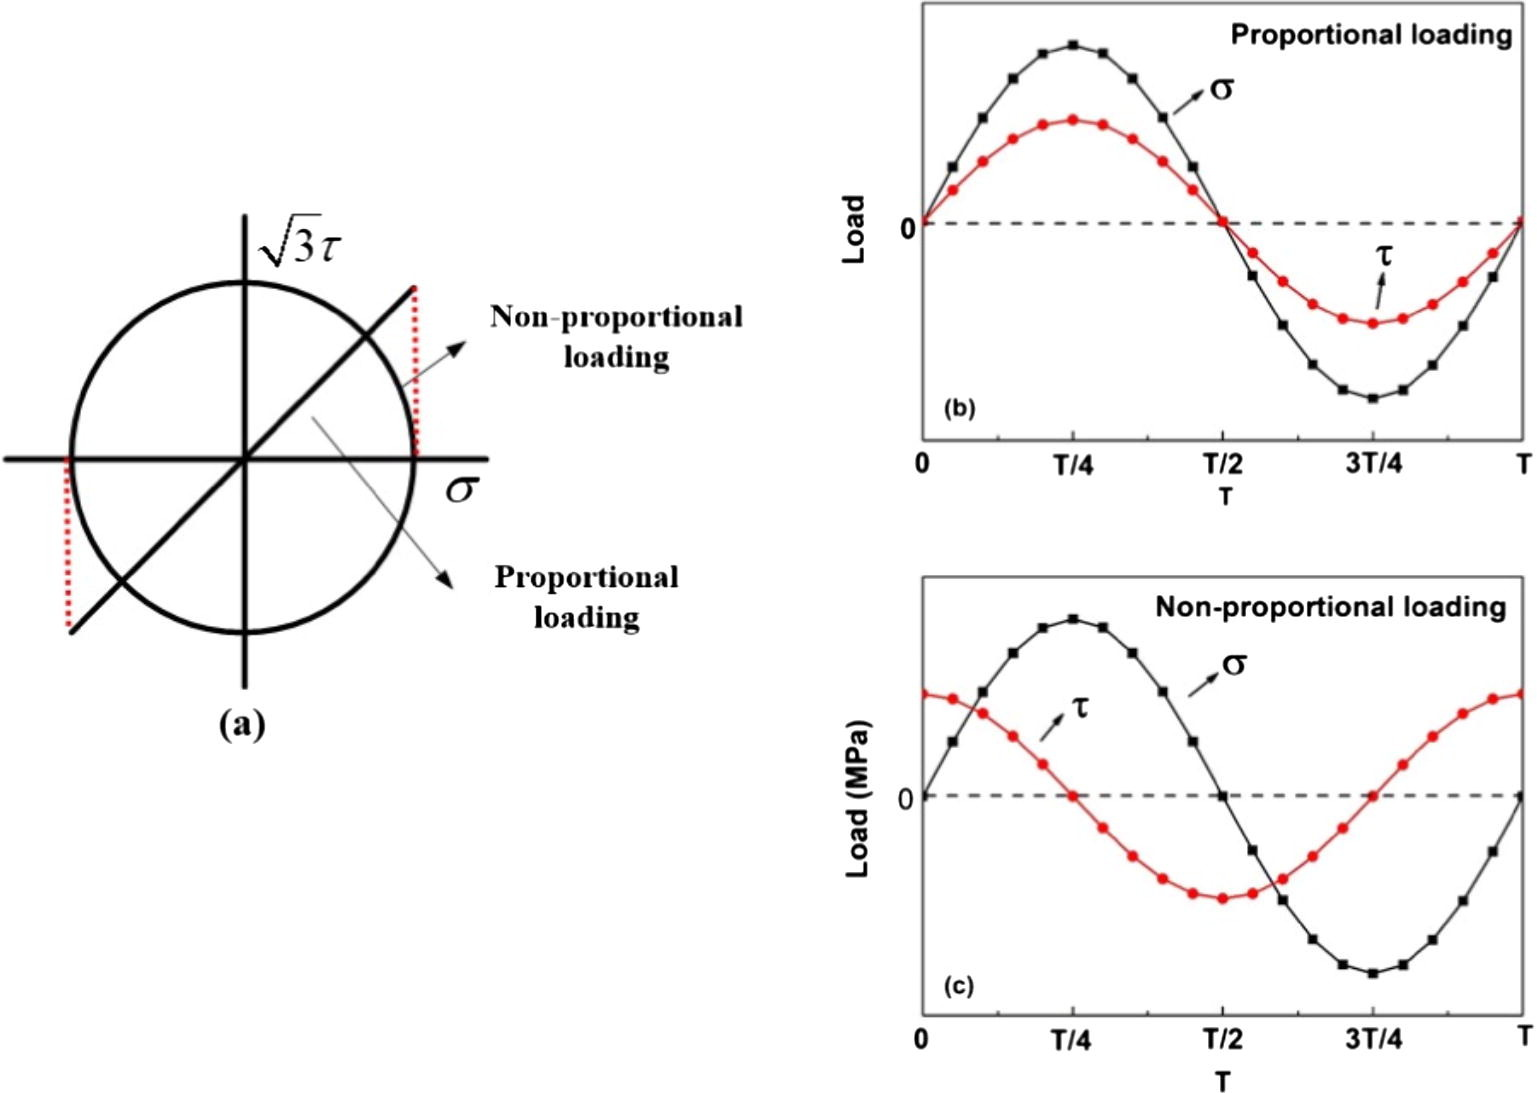
\includegraphics[width=\textwidth]{figures//outofphase.jpg} 
	\caption{The loading path and loading waveform of multiaxial corrosion fatigue (stress control) (a) loading path of proportional and non-proportional, (b) loading waveform of proportional loading, (c) loading waveform of non-proportion (\cite{HUANG2017259})}
	\label{fig.outofphase}
\end{figure}

\begin{figure}[!h]
	\centering
	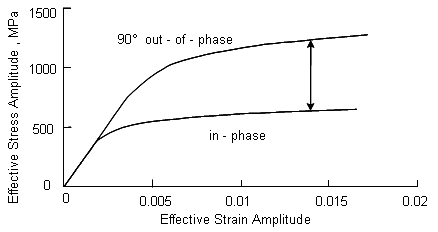
\includegraphics[width=\textwidth]{figures//outofphasestress.png} 
	\caption{The $90^\circ$ out-of-phase loading path has been found to produce the largest degree of non-proportional hardening. (\cite{EFATIGUE})}
	\label{fig.outofphasestress}
\end{figure}

The $90^\circ$ out-of-phase loading path has been found to produce the largest degree of non-proportional hardening. The magnitude of the additional hardening observed for this loading path as compared to that observed in uniaxial or proportional loading is highly dependent on the microstructure and the ease with which slip systems develop in a material. A non-proportional effective stress, $S_{a90}=\sqrt{\sigma_{11}^2+\tau_{12}^2}$, can be introduced which is defined as the equivalent stress under $90^\circ$ out-of-phase loading at high plastic strains in the flat portion of the stress-strain curve. This term reflects the maximum degree of additional hardening that might occur for a given material.



\begin{Figure}[!h]{Calibration on on 6082 T6 aluminum (\cite{susmel2003multiaxial}). Comparison between experimental results and our model used with coefficients given in Tab.\ref{tab.6082T6para}. We obtain a good correlation in bending and torsion tests. The out of phase test are not satisfactory in these batches: P32BT8, P41BT15, P36BT11.}[fig.al6082T6err]
	\graphfile*[52]{figures//AL6082T6_bt1D_err.png}[Bending and torsion tests on 6082 T6 aluminum(R=-1)]
	\graphfile*[52]{figures//AL6082T6_bt2d_err.png}[Bending-torsion tests on 6082 T6 aluminum(R=-1)]
	\\
	\graphfile*[52]{figures//AL6082T6_bt2d90_err.png}[Bending-torsion $90^\circ$ out of phase tests on 6082 T6 aluminum(R=-1)]
\end{Figure}

The model predictive results for the periodic loads of constant amplitude with a radial path are in good agreement with the durations of experimental life. For the latter condition, 90 deg out-of-phase loading was also investigated(\figref{fig.al6082T6err}c). These tests indicated a dramatic change in the number of cycles to failure , $N_F$ , as a result of out-of-phase loading. The influence of the plastic strain path on life is thus clearly demonstrated. It is shown that the total strain energy density, $ΔW_t = ΔW_e+ + ΔW_p$ (\cite{ellyin1991phase}) , correlates with both the in-phase and out-of-phase cyclic tests, and therefore is a proper damage parameter to be used for life predictions. Our microplasticity model does not take this strain path effect into account and we get inaccurate results on this test.



\clearpage
\section{Experimental validation of the model on 30NCD16 steel}
\subsection{Presentation of steel 30NCD16}
Tests with blocks of loading from database are compared to our model predictions. The material for testing is steel 30NCD16. The mechanical characteristics relating to each lot were determined by Dubar (\cite{Dubar1992}) by effecting monotonic tensile test batch. He eventually define ``average material" one who has characteristics listed in Tab.\ref{30ncdchar}:

\begin{table}[!h]
	\centering
	\begin{tabular}{|c|c|c|c|l|c|}
		\hline
		\textbf{$\sigma_{y0.02\%}${[}MPa{]}} & \textbf{$\sigma_{y0.2\%}${[}MPa{]}} & \textbf{$\sigma_u${[}MPa{]}} & \textbf{$\sigma_{-1}${[}MPa{]}} & \textbf{$\tau_{-1}${[}MPa{]}} & \textbf{$E${[}GPa{]}}\\ \hline
		895                                  & 1080                                & 1200                         & 690                             & \multicolumn{1}{c|}{428}     & 191 \\ \hline
	\end{tabular}
	\caption{Mechanical and dynamic characteristics of 30NCD16 steel \cite{Dubar1992}}
	\label{30ncdchar}
\end{table}

\subsection{Fatigue tests performed by Dubar on steel 30 NCD 16}
Tests carried out under simple bending and torsional stresses are grouped together in
Tab.\ref{bendingr1} and \ref{torsionR1}.

\begin{table}[!h]
	\centering
	\begin{tabular}{|c|c|c|c|}
		\hline
		\begin{tabular}[c]{@{}c@{}}Bending Tests\\ (R=-1)\end{tabular} & \begin{tabular}[c]{@{}c@{}}N\\ {[}Cycles{]}\end{tabular} & \begin{tabular}[c]{@{}c@{}}$\sigma_{x,m}$\\ {[}MPa{]}\end{tabular} & \begin{tabular}[c]{@{}c@{}}$\sigma_{x,a}$\\ {[}MPa{]}\end{tabular} \\ \hline
		1 & 51000 & 0 & 820 \\  \hline
		2 & 80000 & 0 & 795 \\  \hline
		3 & 90000 & 0 & 790 \\  \hline
		4 & 95000 & 0 & 785 \\  \hline
		5 & 100000 & 0 & 780 \\  \hline
		6 & 120000 & 0 & 765 \\  \hline
		7 & 140000 & 0 & 752 \\  \hline
		8 & 200000 & 0 & 725 \\  \hline
		9 & 210000 & 0 & 720 \\  \hline
		10 & 230000 & 0 & 715 \\  \hline
		11 & 250000 & 0 & 708 \\ \hline  
	\end{tabular}
	\caption{$30 NCD 16$ steel fully reversed bending tests \cite{Dubar1992}}
	\label{bendingr1}
\end{table}

\begin{table}[!h]
	\centering
	\begin{tabular}{|c|c|c|}
		\hline
		\begin{tabular}[c]{@{}c@{}}Torsion Tests\\ (R=-1)\end{tabular} & \begin{tabular}[c]{@{}c@{}}N\\ {[}Cycles{]}\end{tabular} & \begin{tabular}[c]{@{}c@{}}$\tau_{xy,a}$\\ {[}MPa{]}\end{tabular} \\ \hline
		16 & 51000 & 527 \\ \hline
		17 & 80000 & 505 \\ \hline
		18 & 90000 & 500 \\ \hline
		19 & 95000 & 497 \\ \hline
		20 & 100000 & 495 \\ \hline
		21 & 120000 & 482 \\ \hline
		22 & 140000 & 470 \\ \hline
		23 & 200000 & 450 \\ \hline
		24 & 210000 & 446 \\ \hline
		25 & 230000 & 445 \\ \hline
		26 & 250000 & 440 \\ \hline
	\end{tabular}
	\caption{$30 NCD 16$ steel fully reversed torsion tests (\cite{Dubar1992})}
	\label{torsionR1}
\end{table}

The results of combined bending-torsion tests in phase with or without mean stress $\sigma_{x,m}$ are given in the Tab.\ref{torsionR1} and Tab.\ref{tab.30ncd16bt}:
\begin{table}[!h]
	\centering
	\begin{tabular}{|c|c|c|c|c|}
		\hline
		\begin{tabular}[c]{@{}c@{}}Bending Tests\\ (R=-1)\end{tabular} & \begin{tabular}[c]{@{}c@{}}N\\ {[}Cycles{]}\end{tabular} & \begin{tabular}[c]{@{}c@{}}$\sigma_{x,m}$\\ {[}MPa{]}\end{tabular} & \begin{tabular}[c]{@{}c@{}}$\sigma_{x,a}$\\ {[}MPa{]}\end{tabular} & \begin{tabular}[c]{@{}c@{}}$\tau_{xy,a}$\\ {[}MPa{]}\end{tabular} \\ \hline
		27 & 80000 & 0 & 600 & 335 \\ \hline
		28 & 200000 & 0 & 548 & 306 \\ \hline
		29 & 120000 & 290 & 0 & 460 \\ \hline
		30 & 120000 & 450 & 0 & 460 \\ \hline
		31 & 250000 & 450 & 0 & 430 \\ \hline
		32 & 95000 & 450 & 490 & 285 \\ \hline
		33 & 120000 & 290 & 500 & 290 \\ \hline
	\end{tabular}
	\caption{$30 NCD 16$ steel bending-torsion tests (\cite{Dubar1992})}
	\label{tab.30ncd16bt}
\end{table}

\subsection{Identification of model parameters for steel 30 NCD 16}
The identification of the parameters consists in minimizing the relative difference between the experimental lifetimes and calculated ones for purely alternating bending tests (R = -1). Following the identification strategy of section \ref{sec:5.9}, it is clearly indicated in \figref{fig.30NCD16sn}a by obtaining a good correlation between these different lifetimes

\begin{table}[!h]
	\centering
	\begin{tabular}{|c|c|c|c|c|c|}
		\hline
		\textbf{$\beta$} & \textbf{$\lambda_+$} & \textbf{$\lambda_-$} & \textbf{$W_0$} & \textbf{$a$}& \textbf{$f$}  \\ \hline
		5.3     & 0.55 &0         &4.97E8 Pa  & 0.4& 1.1   \\ \hline
	\end{tabular}
	\caption{Parameter identification of 30NCD16 steel}
	\label{30ncdpara2}
\end{table}

\begin{Figure}[!h]{Calibration on  30NCD16 (\cite{Dubar1992}). We can observe that the bending-torsion experimental values are largely dispersed}[fig.30NCD16sn]
	\graphfile*[52]{figures//NCD16_bt1D_sn.png}[Bending and torsion tests on 30NCD16(R=-1)]
	\graphfile*[52]{figures//NCD16_bt2D_m_sn.png}[Bending-torsion tests with mean stress on 30NCD16]
\end{Figure}

\begin{Figure}[!h]{Calibration on  30NCD16 (\cite{Dubar1992}). In figure (c) data 29(same $N_F$ with data30 but with smaller $\sigma_{x,m}$) and 32(2-D with large mean stress)  from Tab.\ref{tab.30ncd16bt} are more dispersed. The numerical tests are carried out using the coefficients of Tab.\ref{30ncdpara2}}[fig.30NCD16err]
	\graphfile*[52]{figures//NCD16_bt1D_err.png}[Bending and torsion tests on 30NCD16(R=-1)]
	\graphfile*[52]{figures//NCD16_bt2D_m_err.png}[Bending-torsion tests with mean stress on 30NCD16]
\end{Figure}


\clearpage
\section{Experimental validation of the model on SM45C steel}
\subsection{Presentation of steel SM45C}
This is a structural steel widespread use for the crankshafts and the structural components. The chemical composition and mechanical properties of this material is given in Tab. \ref{SM45Cchem} and Tab. \ref{SM45Cmec}.

\begin{table}[!h]
	\centering
	\begin{tabular}{|c|c|c|c|c|c|c|c|}
		\hline
		\textbf{C} & \textbf{Mn} & \textbf{P} & \textbf{S} & \textbf{Si} & \textbf{Ni} & \textbf{Cr} & \textbf{Cu} \\ \hline
		0.42       & 0.73        & 0.02       & 0.012      & 0.28        & 0.14        & 0.18        & 0.13        \\ \hline
	\end{tabular}
	\caption{Chemical composition of SM45C steel}
	\label{SM45Cchem}
\end{table}
\begin{table}[!h]
	\centering
	\begin{tabular}{|c|c|c|c|c|c|}
		\hline
		\textbf{\begin{tabular}[c]{@{}c@{}}$\sigma_{y}$\\ {[}MPa{]}\end{tabular}} & \textbf{\begin{tabular}[c]{@{}c@{}}$\sigma_{u}$\\ {[}MPa{]}\end{tabular}} & \textbf{\begin{tabular}[c]{@{}c@{}}E\\ {[}GPa{]}\end{tabular}} & \textbf{\begin{tabular}[c]{@{}c@{}}G\\ {[}GPa{]}\end{tabular}} & \textbf{$\nu$} & \textbf{A} \\ \hline
		638                                                                       & 824                                                                       & 213                                                            & 82.5                                                           & 0.29           & 22         \\ \hline
	\end{tabular}
	\caption{Mechanical and dynamic characteristics of SM45C steel}
	\label{SM45Cmec}
\end{table}

\begin{flushleft}
	E: Young's modulus,
	
	G: Shear modulus,
	
	$\nu$: Poisson ratio,
	
	A:	Elongation at break.
\end{flushleft}
\newpage
\subsection{Fatigue tests performed by Dubar on steel SM45C}
Preliminary fatigue tests in purely alternating torsion and purely alternating flexion were performed by \cite{lee2013out}. These two types of tests were carried out with test pieces of the same geometric shape. In addition, the author had performed moderate stress bending fatigue tests to study its effect on the lifetime of SM45C steel. All uniaxial fatigue tests performed by \cite{lee2013out} are illustrated in \figref{fig.SM45CSN}. This figure shows a reduction in bending life of SM45C steel in the presence of a positive mean stress. Crack initiation was detected when the stiffness of the specimen or specimen used was reduced by 10\%.
\begin{figure}[!h]
	\centering
	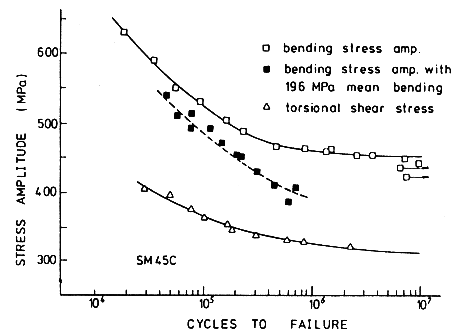
\includegraphics[width=\textwidth]{figures//SM45C_SN.png} 
	\caption{Fatigue curves on SM45C steel by \cite{lee2013out}}
	\label{fig.SM45CSN}
\end{figure}


Preliminary fatigue tests were carried out under fully reversed bending and torsion separately.
\begin{table}[!h]
	\centering
	\begin{tabular}{crrr}
		\hline
		\begin{tabular}[c]{@{}c@{}}Bending Tests\\ (R=-1)\end{tabular}& \begin{tabular}[c]{@{}c@{}}N\\ {[}Cycles{]}\end{tabular} & \begin{tabular}[c]{@{}c@{}}$\sigma_{x,a}$\\ {[}MPa{]}\end{tabular} & \begin{tabular}[c]{@{}c@{}}$\sigma_{x,m}$\\ {[}MPa{]}\end{tabular}\\ 
		\hline
		1 & 17520 & 632.1 & 0 \\
		2 & 33991 & 590.1 & 0 \\
		3 & 52427 & 552.0 & 0 \\
		4 & 91077 & 529.5 & 0 \\
		5 & 156882 & 506.5 & 0 \\
		6 & 222261 & 489.8 & 0 \\
		7 & 446115 & 466.7 & 0 \\
		8 & 822487 & 463.8 & 0 \\
		9 & 1279414 & 459.2 & 0 \\
		10 & 1453321 & 463.8 & 0 \\
		11 & 2440360 & 454.0 & 0 \\
		12 & 3428115 & 455.2 & 0 \\
		13 & 6880791 & 450.0 & 0 \\
		14 & 6213809 & 437.3 & 0 \\
		15 & 9342857 & 441.9 & 0 \\
		16 & 7240667 & 424.1 & 0 \\ \hline
		1 & 43043 & 541.5 & 196 \\
		2 & 55523 & 511.5 & 196 \\
		3 & 74725 & 514.4 & 196\\
		4 & 75362 & 493.6 & 196\\
		5 & 110407 & 490.7 & 196 \\
		6 & 146090 & 471.1 & 196 \\
		7 & 194951 & 455.5 & 196 \\
		8 & 212218 & 452.0 & 196 \\
		9 & 297990 & 430.1 & 196 \\
		10 & 440286 & 409.3 & 196 \\
		11 & 678727 & 407.6 & 196\\
		12 & 597603 & 386.8 & 196 \\ \hline
	\end{tabular}
	\caption{SM45C steel fully reversed bending tests(extracted from  \cite{lee2013out})}
	\label{SM45Cbendingr1}
\end{table}

\begin{table}[!h]
	\centering
	\begin{tabular}{crrr}
		\hline
		\begin{tabular}[c]{@{}c@{}}Torsion Tests\\ (R=-1)\end{tabular} & \begin{tabular}[c]{@{}c@{}}N\\ {[}Cycles{]}\end{tabular} & \begin{tabular}[c]{@{}c@{}}$\tau_{xy,a}$\\ {[}MPa{]}\end{tabular} & \begin{tabular}[c]{@{}c@{}}$\sigma_{x,m}$\\ {[}MPa{]}\end{tabular}\\
		\hline
		1 & 27957 & 404.1 & 0 \\
		2 & 47749 & 394.9 & 0 \\
		3 & 76194 & 375.3 & 0 \\
		4 & 100000 & 363.1 & 0 \\
		5 & 162305 & 354.5 & 0 \\
		6 & 182807 & 345.8 & 0 \\
		7 & 296705 & 338.3 & 0 \\
		8 & 575636 & 331.4 & 0 \\
		9 & 822487 & 329.1 & 0 \\
		10 & 2203806 & 322.2 & 0 \\ \hline
	\end{tabular}
	\caption{SM45 steel fully reversed torsion tests(extracted from  \cite{lee2013out})}
	\label{SM45CtorsionR1}
\end{table}



\begin{table}[!h]
	\centering
	\begin{tabularx}{\textwidth}{XXXXX}
		\hline
		\textbf{Group}               & \multicolumn{1}{l}{\textbf{\begin{tabular}[l]{@{}c@{}}N\\ {[}Cycles{]}\end{tabular}}} & \multicolumn{1}{l}{\textbf{\begin{tabular}[l]{@{}c@{}}$\tau_a$\\ {[}MPa{]}\end{tabular}}} & \multicolumn{1}{l}{\textbf{\begin{tabular}[l]{@{}c@{}}$\sigma_a$\\ {[}MPa{]}\end{tabular}}} & \multicolumn{1}{l}{\textbf{\begin{tabular}[l]{@{}c@{}}$\sigma_m$\\ {[}MPa{]}\end{tabular}}} \\ \hline
		\multirow{10}{*}{\textbf{A}} & 29.9E3                                                                                & 282                                                                                       & 449                                                                                         & 0                                                                                           \\
		& 35.7E3                                                                                & 334                                                                                       & 354                                                                                         & 0                                                                                           \\
		& 50E3                                                                                  & 223                                                                                       & 485                                                                                         & 0                                                                                           \\
		& 73.8E3                                                                                & 309                                                                                       & 357                                                                                         & 0                                                                                           \\
		& 106E3                                                                                 & 217                                                                                       & 449                                                                                         & 0                                                                                           \\
		& 106E3                                                                                 & 285                                                                                       & 370                                                                                         & 0                                                                                           \\
		& 112E3                                                                                 & 199                                                                                       & 449                                                                                         & 0                                                                                           \\
		& 131E3                                                                                 & 194                                                                                       & 457                                                                                         & 0                                                                                           \\
		& 333E3                                                                                 & 252                                                                                       & 354                                                                                         & 0                                                                                           \\
		& 431E3                                                                                 & 154                                                                                       & 437                                                                                         & 0                                                                                           \\ \hline
		\multirow{10}{*}{\textbf{B}} & 53E3                                                                                  & 215                                                                                       & 441                                                                                         & 196                                                                                         \\
		& 59.2E3                                                                                & 309                                                                                       & 286                                                                                         & 196                                                                                         \\
		& 70.1E3                                                                                & 155                                                                                       & 464                                                                                         & 196                                                                                         \\
		& 86.3E3                                                                                & 136                                                                                       & 473                                                                                         & 196                                                                                         \\
		& 89.9E3                                                                                & 334                                                                                       & 173                                                                                         & 196                                                                                         \\
		& 92.1E3                                                                                & 209                                                                                       & 403                                                                                         & 196                                                                                         \\
		& 102E3                                                                                 & 177                                                                                       & 437                                                                                         & 196                                                                                         \\
		& 135E3                                                                                 & 321                                                                                       & 167                                                                                         & 196                                                                                         \\
		& 351E3                                                                                 & 179                                                                                       & 357                                                                                         & 196                                                                                         \\
		& 394E3                                                                                 & 274                                                                                       & 182                                                                                         & 196                                                                                         \\ \hline
	\end{tabularx}
	\caption{Effect of mean bending stress on out-of-phase($90^\circ$) fatigue of SM45C steel (\cite{lee2013out})}
	\label{meanSM45C}
\end{table}

\newpage
\subsection{Identification of model parameters for steel SM45C}

We use the same identification strategy as described in Section \ref{sec:5.9}. The fitted curve using experimental data in Tab.\ref{meanSM45C} and data with mean stress effect is shown in \figref{fig.SM45C}b.
The tests on SM45C steel have illustrated that the mean bending stress has an influence on both uniaxial and multiaxial fatigue life. 

Although the uniaxial experimental data we extracted from Lee's curve (\cite{lee2013out}) of SM45C steel are slightly dispersed, we can find our model quite satisfactory in the case of SM45C steel. As for multiaxial 90 degree out of phase, fully reversed bending-torsion fatigue tests, our model is able to evaluate the cycles to failure.

\begin{table}[!h]
	\centering
	\begin{tabular}{|c|c|c|c|c|c|}
		\hline
		\textbf{$\beta(LCF/HCF)$} & \textbf{$\lambda_+$} & \textbf{$\lambda_-$} & \textbf{$W_0(LCF/HCF)$} & \textbf{$a$}& \textbf{$f$}  \\ \hline
		6/15.8  & 1.4 &0         &2.6E8/5.6E5 Pa  & 0.1 & 1.1    \\ \hline
	\end{tabular}
	\caption{Parameter identification of SM45C steel}
	\label{sm45cpara}
\end{table}

\begin{Figure}[!h]{Calibration on  SM45C}[fig.SM45C]
	\graphfile*[52]{figures//SM45C_bt1D_sn.png}[Bending and torsion test on SM45C steel(R=-1)]
	\graphfile*[52]{figures//SM45C_b1D_m_sn.png}[Bending test with mean stress on SM45C steel ($\sigma_m=196 MPa$)]
	\\
	\graphfile*[52]{figures//SM45C_bt2D90_sn.png}[Bending-torsion 90 degree out-of-phase tests on SM45C steel]
	\graphfile*[52]{figures//SM45C_bt2D90_m_sn.png}[Bending-torsion 90 degree out-of-phase tests with mean stress on SM45C steel]
\end{Figure}

\begin{Figure}[!h]{Calibration on  SM45C. The numerical tests are carried out using the coefficients of Tab.\ref{sm45cpara}}[fig.SM45C]
	\graphfile*[52]{figures//SM45C_bt1D_err.png}[Bending and torsion test on SM45C steel (R=-1)]
	\graphfile*[52]{figures//SM45C_b1D_m_err.png}[Bending test with mean stress on SM45C steel ($\sigma_m=196 MPa$)]
	\\
	\graphfile*[52]{figures//SM45C_bt2D90_err.png}[Bending-torsion 90 degree out-of-phase tests on SM45C steel]
	\graphfile*[52]{figures//SM45C_bt2D90_m_err.png}[Bending-torsion 90 degree out-of-phase tests with mean stress on SM45C steel]
\end{Figure}


\clearpage
\section{Experimental validation of the model on 10 HNAP steel}
\subsection{Presentation of the material}
Fatigue tests were performed on the HNAP steel. It is a very low carbon steel
which resembles the 10 CN 6. In Tab.\ref{tab.10HNAPchem}, its chemical composition is given:	
\begin{table}[!h]
	\centering
	\begin{tabular}{rrrrrrrrr}
		\hline
		C      & Mn     & Si     & P      & S      & Cr     & Cu     & Ni     & Fe       \\
		0.12\% & 0.71\% & 0.41\% & 0.08\% & 0.03\% & 0.81\% & 0.30\% & 0.50\% & the rest \\ \hline
	\end{tabular}
	\caption{Chemical composition of 10 HNAP steel, data from \cite{Bedkowski1994}}
	\label{tab.10HNAPchem}
\end{table}
The mechanical properties of this steel are given in Tab.\ref{tab.10HNAPmec}:
\begin{table}[!h]
	\centering
	\begin{tabular}{rrrrr}
		\hline
		$Re_{0.2\%}$ & $R_m$   & A    & $\nu$ & E          \\
		418 MPa     & 566 Mpa & 32\% & 0.29  & 215000 Mpa \\ \hline
	\end{tabular}
	\caption{Mechanical characteristics of steel 10 HNAP, data from \cite{Bedkowski1994}}
	\label{tab.10HNAPmec}
\end{table}

where 
\begin{table}[!h]
	\centering
	\begin{tabular}{ll}
		$Re_{0.2\%}$ & : elastic limit at 0.2\% of plastic deformation, \\
		$R_m$      & : maximum tensile strength,                                                                  \\
		A          & : elongation at break,                                                                       \\
		$\nu$      & : Poisson's coefficient,                                                                     \\
		E          & : Young's modulus.                                                                          
	\end{tabular}
\end{table}

\subsection{Description of fatigue tests on 10 HNAP steel}
The Macha team performed a large number of fatigue tests on the HNAP steel. Thus, it performed not only simple tensile compression and torsion tests (R = -1) in order to establish the corresponding Wöhler curves but also tests under variable loading on cylindrical specimens of the same material (\cite{ACHTELIC1994}). \cite{VIDAL1996} carried out tensile tests on this material for various mean stress values. It has established the Wöhler curve in repeated traction in order to validate on this steel the method of Robert whose use requires three Wöhler curves in symmetrical alternating traction, symmetrical alternating torsion and repetitive traction.

\vspace{6pt}
\noindent
\textbf{Wöhler curve in tension-compression}

The model chosen by Macha and recovered by  \cite{jabbado:pastel-00002116} for the tensile-compression Wöhler curve is that of Basquin:
\begin{equation}
lnN=68.361 − 9.82ln\left( \sigma_{-1}\right) ,
\end{equation}

\noindent
\vspace{6pt}
\textbf{Wöhler curve in symmetrical alternating torsion}
\vspace{6pt}

The symmetric alternating torsion Wöhler curve was recovered by \cite{jabbado:pastel-00002116} using following equation:
\begin{equation}
lnN=21.55 − 0.0385\tau_{-1}.
\end{equation}

\noindent
\vspace{6pt}
\textbf{Tensile fatigue tests for various mean stress values}
\vspace{6pt}

\cite{VIDAL1996} carried out tensile tests on HNAP steel for various values of mean stress. The results are summarized in Tab.\ref{tab.10HNAPmean}. They allowed us to plot the Wöhler curves for different values of the mean stress $\sigma_m$. 

\begin{table}[!h]
	\centering
	\begin{tabular}{r|rr|rr|rr|rr}
		\hline
		$N_F$    & $\Sigma_{xx,a}$ & $\sigma_m$ & $\Sigma_{xx,a}$ & $\sigma_m$ & $\Sigma_{xx,a}$ & $\sigma_m$ & $\Sigma_{xx,a}$ & $\sigma_m$ \\ \hline
		1.00E+05 & 311.30          & 75         & 224.42          & 150        & 257.98          & 225        & 251.82          & 300        \\
		2.00E+05 & 289.36          & 75         & 208.40          & 150        & 242.47          & 225        & 224.42          & 300        \\
		3.00E+05 & 276.53          & 75         & 197.03          & 150        & 233.40          & 225        & 208.40          & 300        \\
		4.00E+05 & 267.43          & 75         & 188.21          & 150        & 226.96          & 225        & 197.03          & 300        \\
		5.00E+05 & 260.37          & 75         & 181.00          & 150        & 221.97          & 225        & 188.21          & 300        \\
		6.00E+05 & 254.60          & 75         & 174.91          & 150        & 217.89          & 225        & 181.00          & 300        \\
		7.00E+05 & 249.72          & 75         & 169.63          & 150        & 214.44          & 225        & 174.91          & 300        \\
		8.00E+05 & 245.49          & 75         & 164.97          & 150        & 211.46          & 225        & 169.63          & 300        \\
		9.00E+05 & 241.77          & 75         & 160.81          & 150        & 208.82          & 225        & 164.97          & 300        \\
		1.00E+06 & 238.43          & 75         & 233.29          & 150        & 206.47          & 225        & 160.81          & 300        \\ \hline
	\end{tabular}
	\caption{Experimental results of tensile tests for various values of $\sigma_m$, data from \cite{VIDAL1996}}
	\label{tab.10HNAPmean}
\end{table}

\noindent
\vspace{6pt}
\textbf{Fatigue testing under variable loading}
\vspace{6pt}

Random multiaxial loading fatigue tests were performed on cylindrical HNAP steel specimens (\cite{ACHTELIC1994}). The load considered is proportional and results from a combination of bending and torsion. The random signal is stationary and has a normal distribution as a probability distribution. Tests of this type have been analyzed and simulated by Carpinteri et al. (\cite{carpinteri2003multiaxial}). They were provided to us in the form of tests carried out on the HNAP steel for two values of the angle $\alpha'$: $\alpha' = \pi / 8$ and $\alpha' = \pi / 4$ . $\alpha' $ is the angle made by the resultant moment $M$ with the bending moment $M_B$ (see \figref{fig.10HNAPsample}). The angle is kept constant during each individual test. 

\begin{figure}[!h]
	\centering
	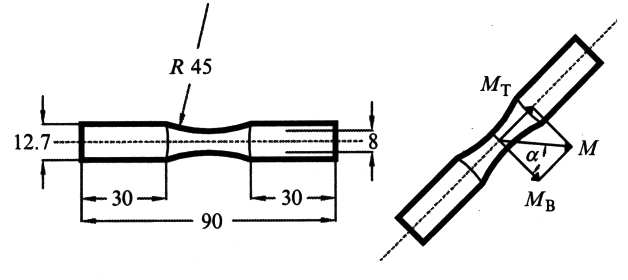
\includegraphics[width=0.8\textwidth]{figures//10HNAPsample.png} 
	\caption{Bending-torsion fatigue tests on cylindrical specimens (\cite{carpinteri2003multiaxial})}
	\label{fig.10HNAPsample}
\end{figure}

The stationary random loading sequence contains 49152 values recorded by a time interval of 0.00375 seconds (frequency = 266.67 Hz). It is shown in \figref{fig.10HNAPrandom}. Its total duration is 184.32 seconds. This sequence is multiplied by load coefficients corresponding to bending $f (\sigma_{xx})$ and torsion $f (\tau_{xy})$ in order to obtain random multiaxial loading sequences. As the signal is stationary, the breaking life is determined in terms of number of sequences with break $N_{Sq}$. Knowing $N_{Sq}$ and the total time in seconds of the sequence studied, it is easy to express the lifetime of the piece in seconds. The results of fatigue tests under variable loads are summarized in Tab.\ref{tab.10HNAPrand1} and Tab.\ref{tab.10HNAPrand2} as a function of angle $\alpha'$ and ratio r; $r =f(\tau_{xy})/f(\sigma_{xx})$.
\begin{figure}[!h]
	\centering
	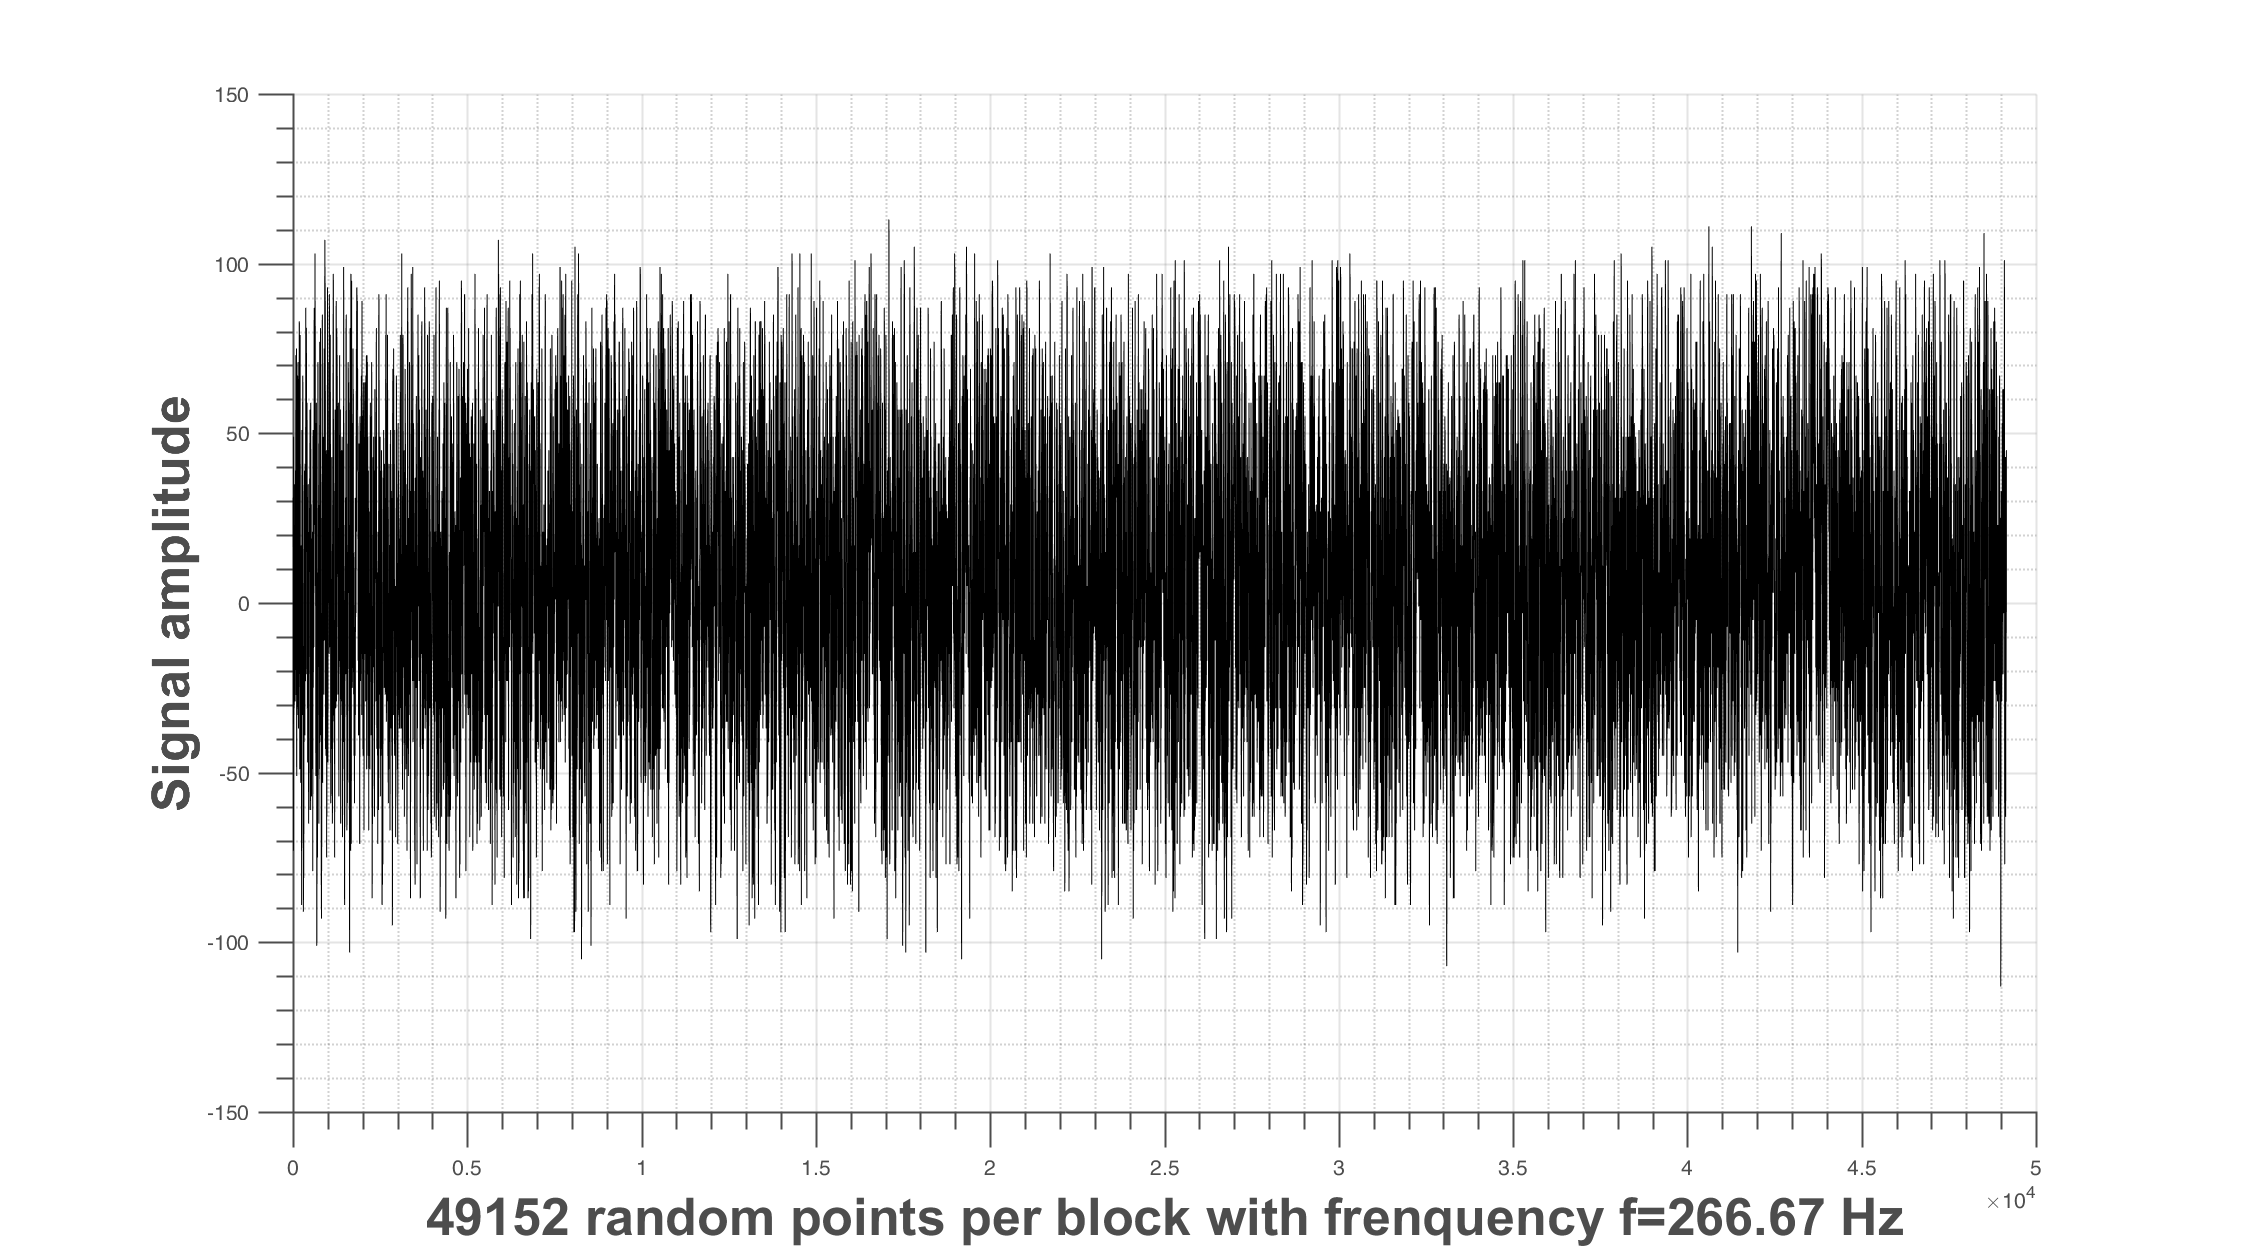
\includegraphics[width=\textwidth]{figures//10HNAPrandomblock.png} 
	\caption{Bending-torsion fatigue tests on cylindrical specimens (\cite{carpinteri2003multiaxial})}
	\label{fig.10HNAPrandom}
\end{figure}

\textbf{1st type of tests:} $\alpha' = \pi / 8$ and $r =f(\tau_{xy})/f(\sigma_{xx})=0.2$.

\begin{table}[!h]
	\centering
	\begin{tabular}{lrrrr}
		\hline
		$N^o$ & $f(\sigma_{xx})$ & $f(\tau_{xy})$ & $r$   & $T_{exp}(s)$ \\ \hline
		1     & 5.7084                  & 1.1822  & 0.2 & 16843.2    \\
		2     & 5.2917                  & 1.0959  & 0.2 & 17780.1    \\
		3     & 4.8337                  & 1.0010  & 0.2 & 24416.5    \\
		4     & 5.2674                  & 1.0909  & 0.2 & 24858.2    \\
		5     & 5.4534                  & 1.1294  & 0.2 & 26518.3    \\
		6     & 5.2002                  & 1.0769  & 0.2 & 36162.3    \\
		7     & 4.7944                  & 0.9929  & 0.2 & 47600.4    \\
		8     & 4.3862                  & 0.9084  & 0.2 & 57993.9    \\
		9     & 4.6241                  & 0.9576  & 0.2 & 60428      \\
		10    & 4.0194                  & 0.8324  & 0.2 & 73373.3    \\
		11    & 4.0127                  & 0.8310  & 0.2 & 87609.1    \\
		12    & 4.2292                  & 0.8758  & 0.2 & 89185.2    \\
		13    & 3.9213                  & 0.8121  & 0.2 & 106900     \\
		14    & 3.7731                  & 0.7814  & 0.2 & 117358     \\
		15    & 4.1148                  & 0.8521  & 0.2 & 118902     \\
		16    & 3.6150                  & 0.7486  & 0.2 & 132448     \\
		17    & 3.3135                  & 0.6862  & 0.2 & 170571     \\
		18    & 4.1298                  & 0.8553  & 0.2 & 178215     \\
		19    & 3.4761                  & 0.7199  & 0.2 & 225288     \\
		20    & 3.3430                  & 0.6923  & 0.2 & 352635     \\
		21    & 3.0135                  & 0.6241  & 0.2 & 355720     \\ \hline
	\end{tabular}
	\caption{Fatigue results under variable loads for $\alpha' = \pi / 8$ and $r =f(\tau_{xy})/f(\sigma_{xx})=0.2$}
	\label{tab.10HNAPrand1}
\end{table}

\textbf{2nd type of tests:} $\alpha' = \pi / 4$ and $r =f(\tau_{xy})/f(\sigma_{xx})=0.5$.

\begin{table}[]
	\centering
	\begin{tabular}{lrrrr}
		\hline
		$N^o$ & $f(\sigma_{xx})$ & $f(\tau_{xy})$ & $r$   & $T_{exp}(s)$ \\ \hline
		1   & 4.2519                  & 2.126   & 0.5 & 15379.4    \\
		2   & 4.0567                  & 2.0284  & 0.5 & 21465.7    \\
		3   & 3.8982                  & 1.9491  & 0.5 & 25350.4    \\
		4   & 3.7823                  & 1.8912  & 0.5 & 45949      \\
		5   & 3.5963                  & 1.7982  & 0.5 & 62434.8    \\
		6   & 3.4497                  & 1.7249  & 0.5 & 75225.7    \\
		7   & 2.9423                  & 1.4712  & 0.5 & 115009     \\
		8   & 2.8814                  & 1.4407  & 0.5 & 136794     \\
		9   & 2.3299                  & 1.165   & 0.5 & 203365     \\
		10  & 2.8399                  & 1.42    & 0.5 & 221370     \\
		11  & 2.8493                  & 1.4247  & 0.5 & 244757     \\
		12  & 2.2542                  & 1.1271  & 0.5 & 251723     \\
		13  & 2.3651                  & 1.1826  & 0.5 & 288080     \\
		14  & 2.4215                  & 1.2108  & 0.5 & 405444     \\ \hline
	\end{tabular}
	\caption{Fatigue results under variable loads for $\alpha' = \pi / 4$ and $r =f(\tau_{xy})/f(\sigma_{xx})=0.5$}
	\label{tab.10HNAPrand2}
\end{table}

In \figref{fig.10HNAP2Drandom}, an example of a random multiaxial loading sequence is given.
\begin{figure}[!h]
	\centering
	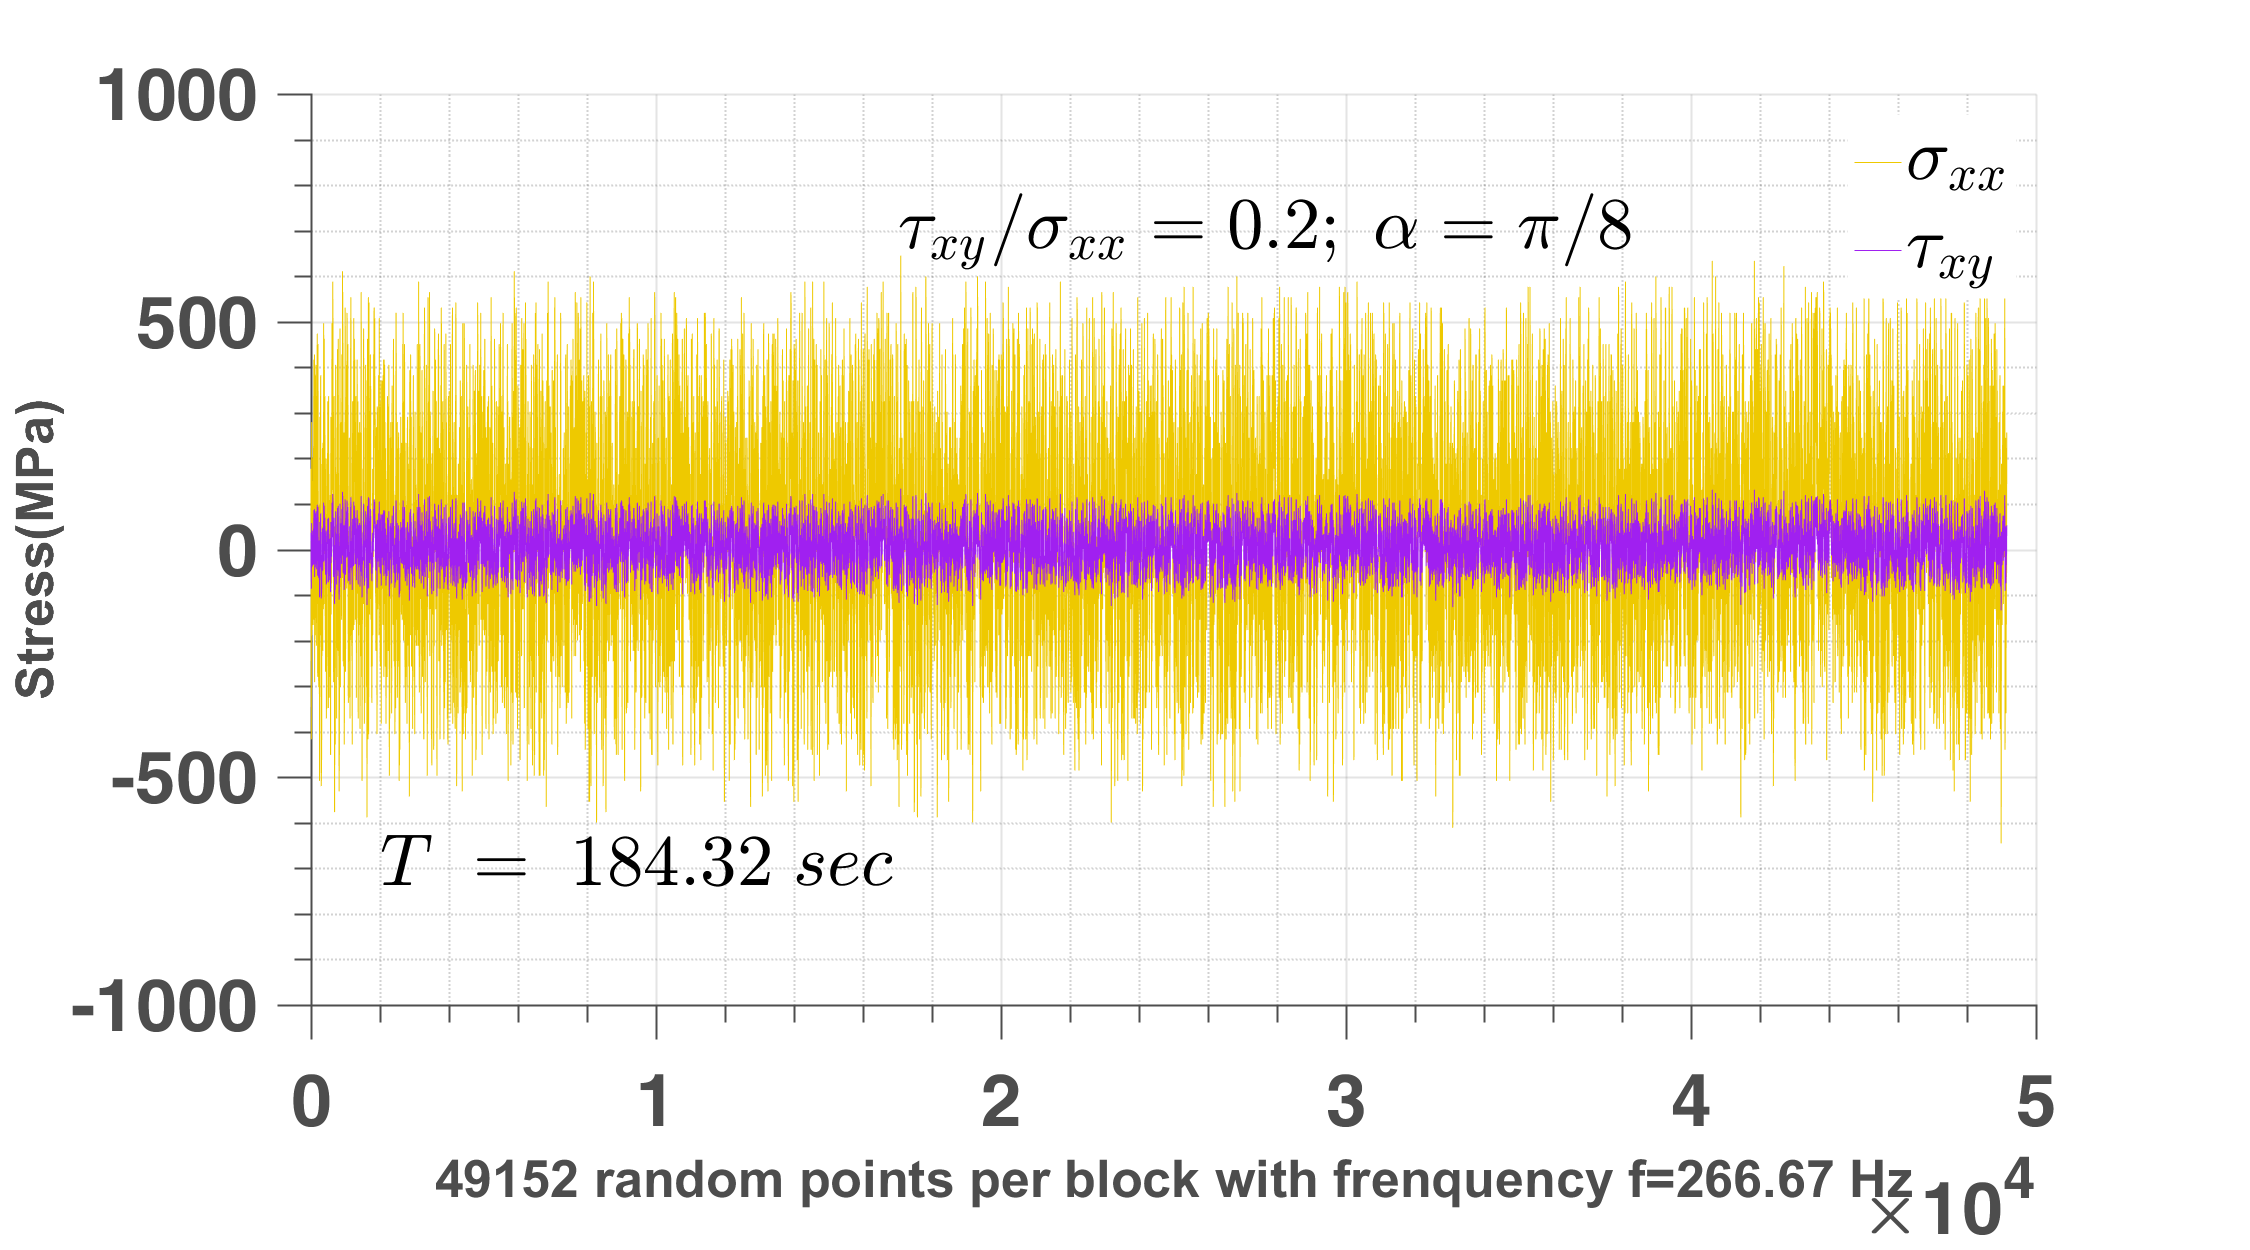
\includegraphics[width=\textwidth]{figures//HNAP_random.png} 
	\caption{Multiaxial random loading sequence}
	\label{fig.10HNAP2Drandom}
\end{figure}

\subsection{Identification of model parameters of 10HNAP steel}
As the previous tests, we identify the slope $\beta$ in pure torsion tests without the mean stress effect. Then fit $\lambda_+$ and $W_0$ with bending tests($R=-1$). The parameters of the HNAP steel model can be identified by referring to Tab.\ref{tab.10HNAP.para}. They are grouped in Tab.\ref{tab.10HNAP.para}:
\begin{table}[!h]
	\centering
	\begin{tabular}{|c|c|c|c|c|c|}
		\hline
		\textbf{$\beta$} & \textbf{$\lambda_+$} & \textbf{$\lambda_-$} & \textbf{$W_0$} & \textbf{$a$} & \textbf{$f$} \\ \hline
		5.3    & 1.7 &0         &6.48E8 Pa  & 0.4   & 1.1 \\ \hline
	\end{tabular}
	\caption{Model parameters for 10HNAP steel}
	\label{tab.10HNAP.para}
\end{table}

The constant amplitude loading tests corresponds to number of cycles to failure in the range of $1E5\sim1E6$. However, in random loading case, the total reversals to failure are $2E6\sim5E7$ (calculated from Tab.\ref{tab.10HNAPrand1} and \ref{tab.10HNAPrand2}). These two cases belongs to different mechanisms, so their sensitivity of sequence effect and mean stress effect can be different as shown in Tab.\ref{tab.10HNAP.para} and \ref{tab.10HNAP.para.random}.

\begin{table}[!h]
	\centering
	\begin{tabular}{|c|c|c|c|c|c|}
		\hline
		\textbf{$\beta$} & \textbf{$\lambda_+$} & \textbf{$\lambda_-$} & \textbf{$W_0$} & \textbf{$a$} & \textbf{$f$} \\ \hline
		5.3    & 0.3 &0         &2.2E8 Pa  & 0.001   & 1.1 \\ \hline
	\end{tabular}
	\caption{Model parameters for 10HNAP steel (random loading)}
	\label{tab.10HNAP.para.random}
\end{table}

\newpage
\subsection{Simulation of fatigue tests performed on 10HNAP steel}
The constant amplitude unidimensional tests data are show in Tab.\ref{tab.10HNAPbending} and \ref{tab.10HNAPtorsion}.

\begin{table}[!h]
	\centering
	\begin{tabular}{ccc}
		\hline
		$N^o$ & $N_{F}$  & $\Sigma_{xx,a}$ \\ \hline
		1     & 1.00E+05 & 326.69     \\
		2     & 2.00E+05 & 304.42     \\
		3     & 3.00E+05 & 292.11     \\
		4     & 4.00E+05 & 283.68     \\
		5     & 5.00E+05 & 277.30     \\
		6     & 6.00E+05 & 272.20     \\
		7     & 7.00E+05 & 267.96     \\
		8     & 8.00E+05 & 264.34     \\
		9     & 9.00E+05 & 261.19     \\
		10    & 1.00E+06 & 258.41     \\ \hline
	\end{tabular}
	\caption{Constant amplitude bending tests performed on 10HNAP steel, data from \cite{VIDAL1996}}
	\label{tab.10HNAPbending}
\end{table}

\begin{table}[!h]
	\centering
	\begin{tabular}{ccc}
		\hline
		$N^o$ & $N_{F}$  & $\Sigma_{xy,a}$ \\ \hline
		1     & 1.00E+05 & 260.70          \\
		2     & 2.00E+05 & 242.70          \\
		3     & 3.00E+05 & 232.17          \\
		4     & 4.00E+05 & 224.70          \\
		5     & 5.00E+05 & 218.90          \\
		6     & 6.00E+05 & 214.16          \\
		7     & 7.00E+05 & 210.16          \\
		8     & 8.00E+05 & 206.69          \\
		9     & 9.00E+05 & 203.63          \\
		10    & 1.00E+06 & 200.90          \\ \hline
	\end{tabular}
	\caption{Constant amplitude torsion tests performed on 10HNAP steel, data from \cite{VIDAL1996}}
	\label{tab.10HNAPtorsion}
\end{table}


After determining the parameters of the 10HNAP steel model for each of the batches tested, the number of priming cycles can be obtained by directly applying equation \eqref{eq.cycNF} for the proportional periodic loads of constant amplitude and for multiaxial loadings of variable amplitude.
\begin{figure}[!h]
	\centering
	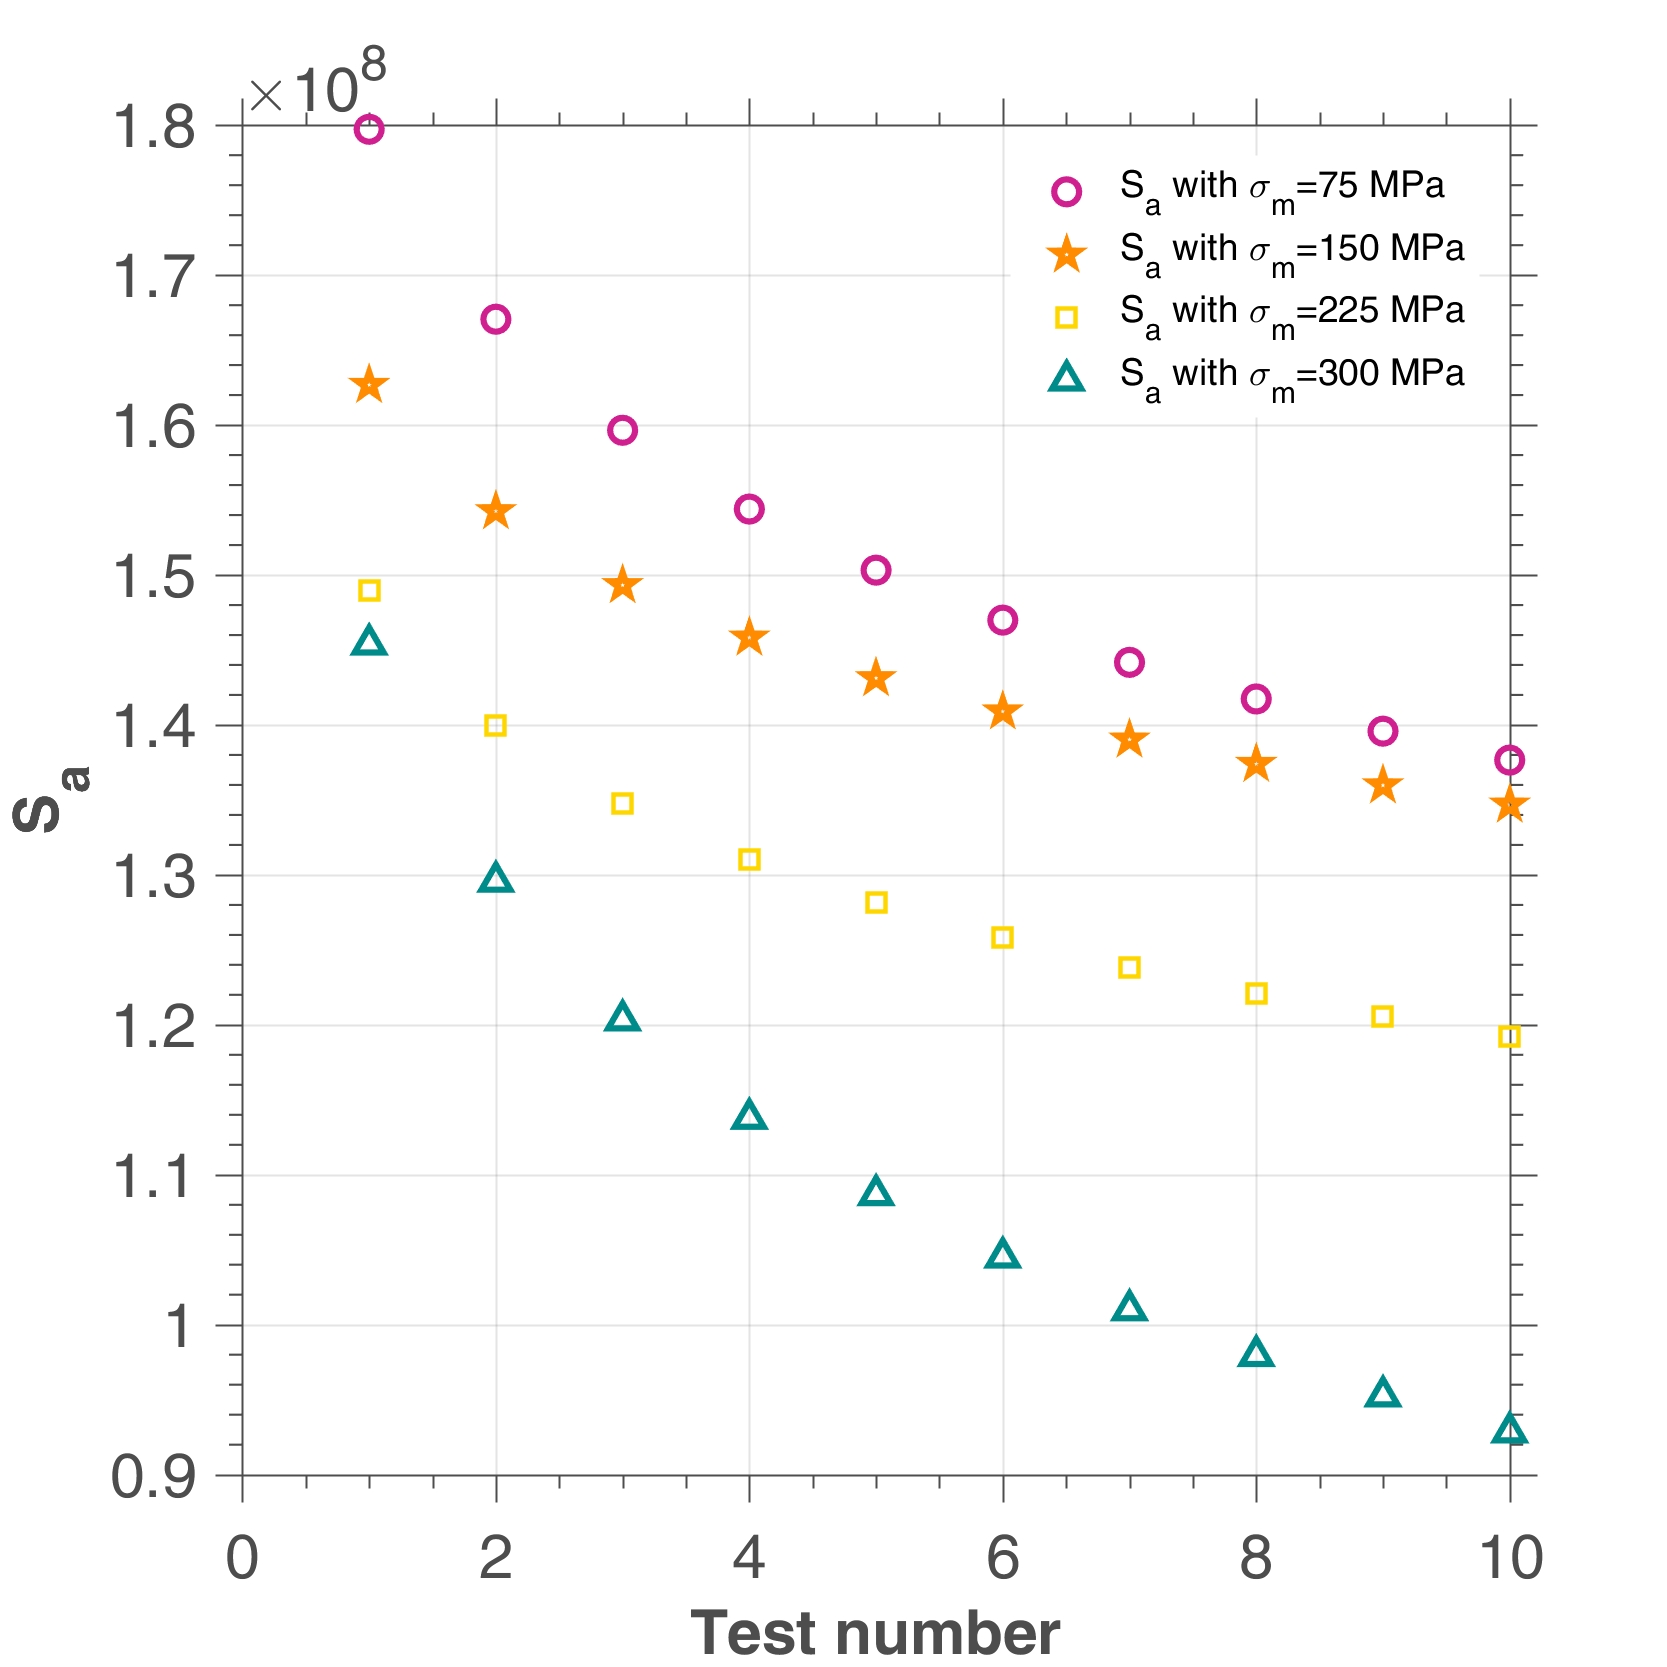
\includegraphics[width=\textwidth]{figures//10HNAP_b1D_m_Smax.png} 
	\caption{$S_{a}$ of bending tests with mean stress on 10HNAP}
	\label{fig.10HNAPSmax}
\end{figure}
\begin{figure}[!h]
	\centering
	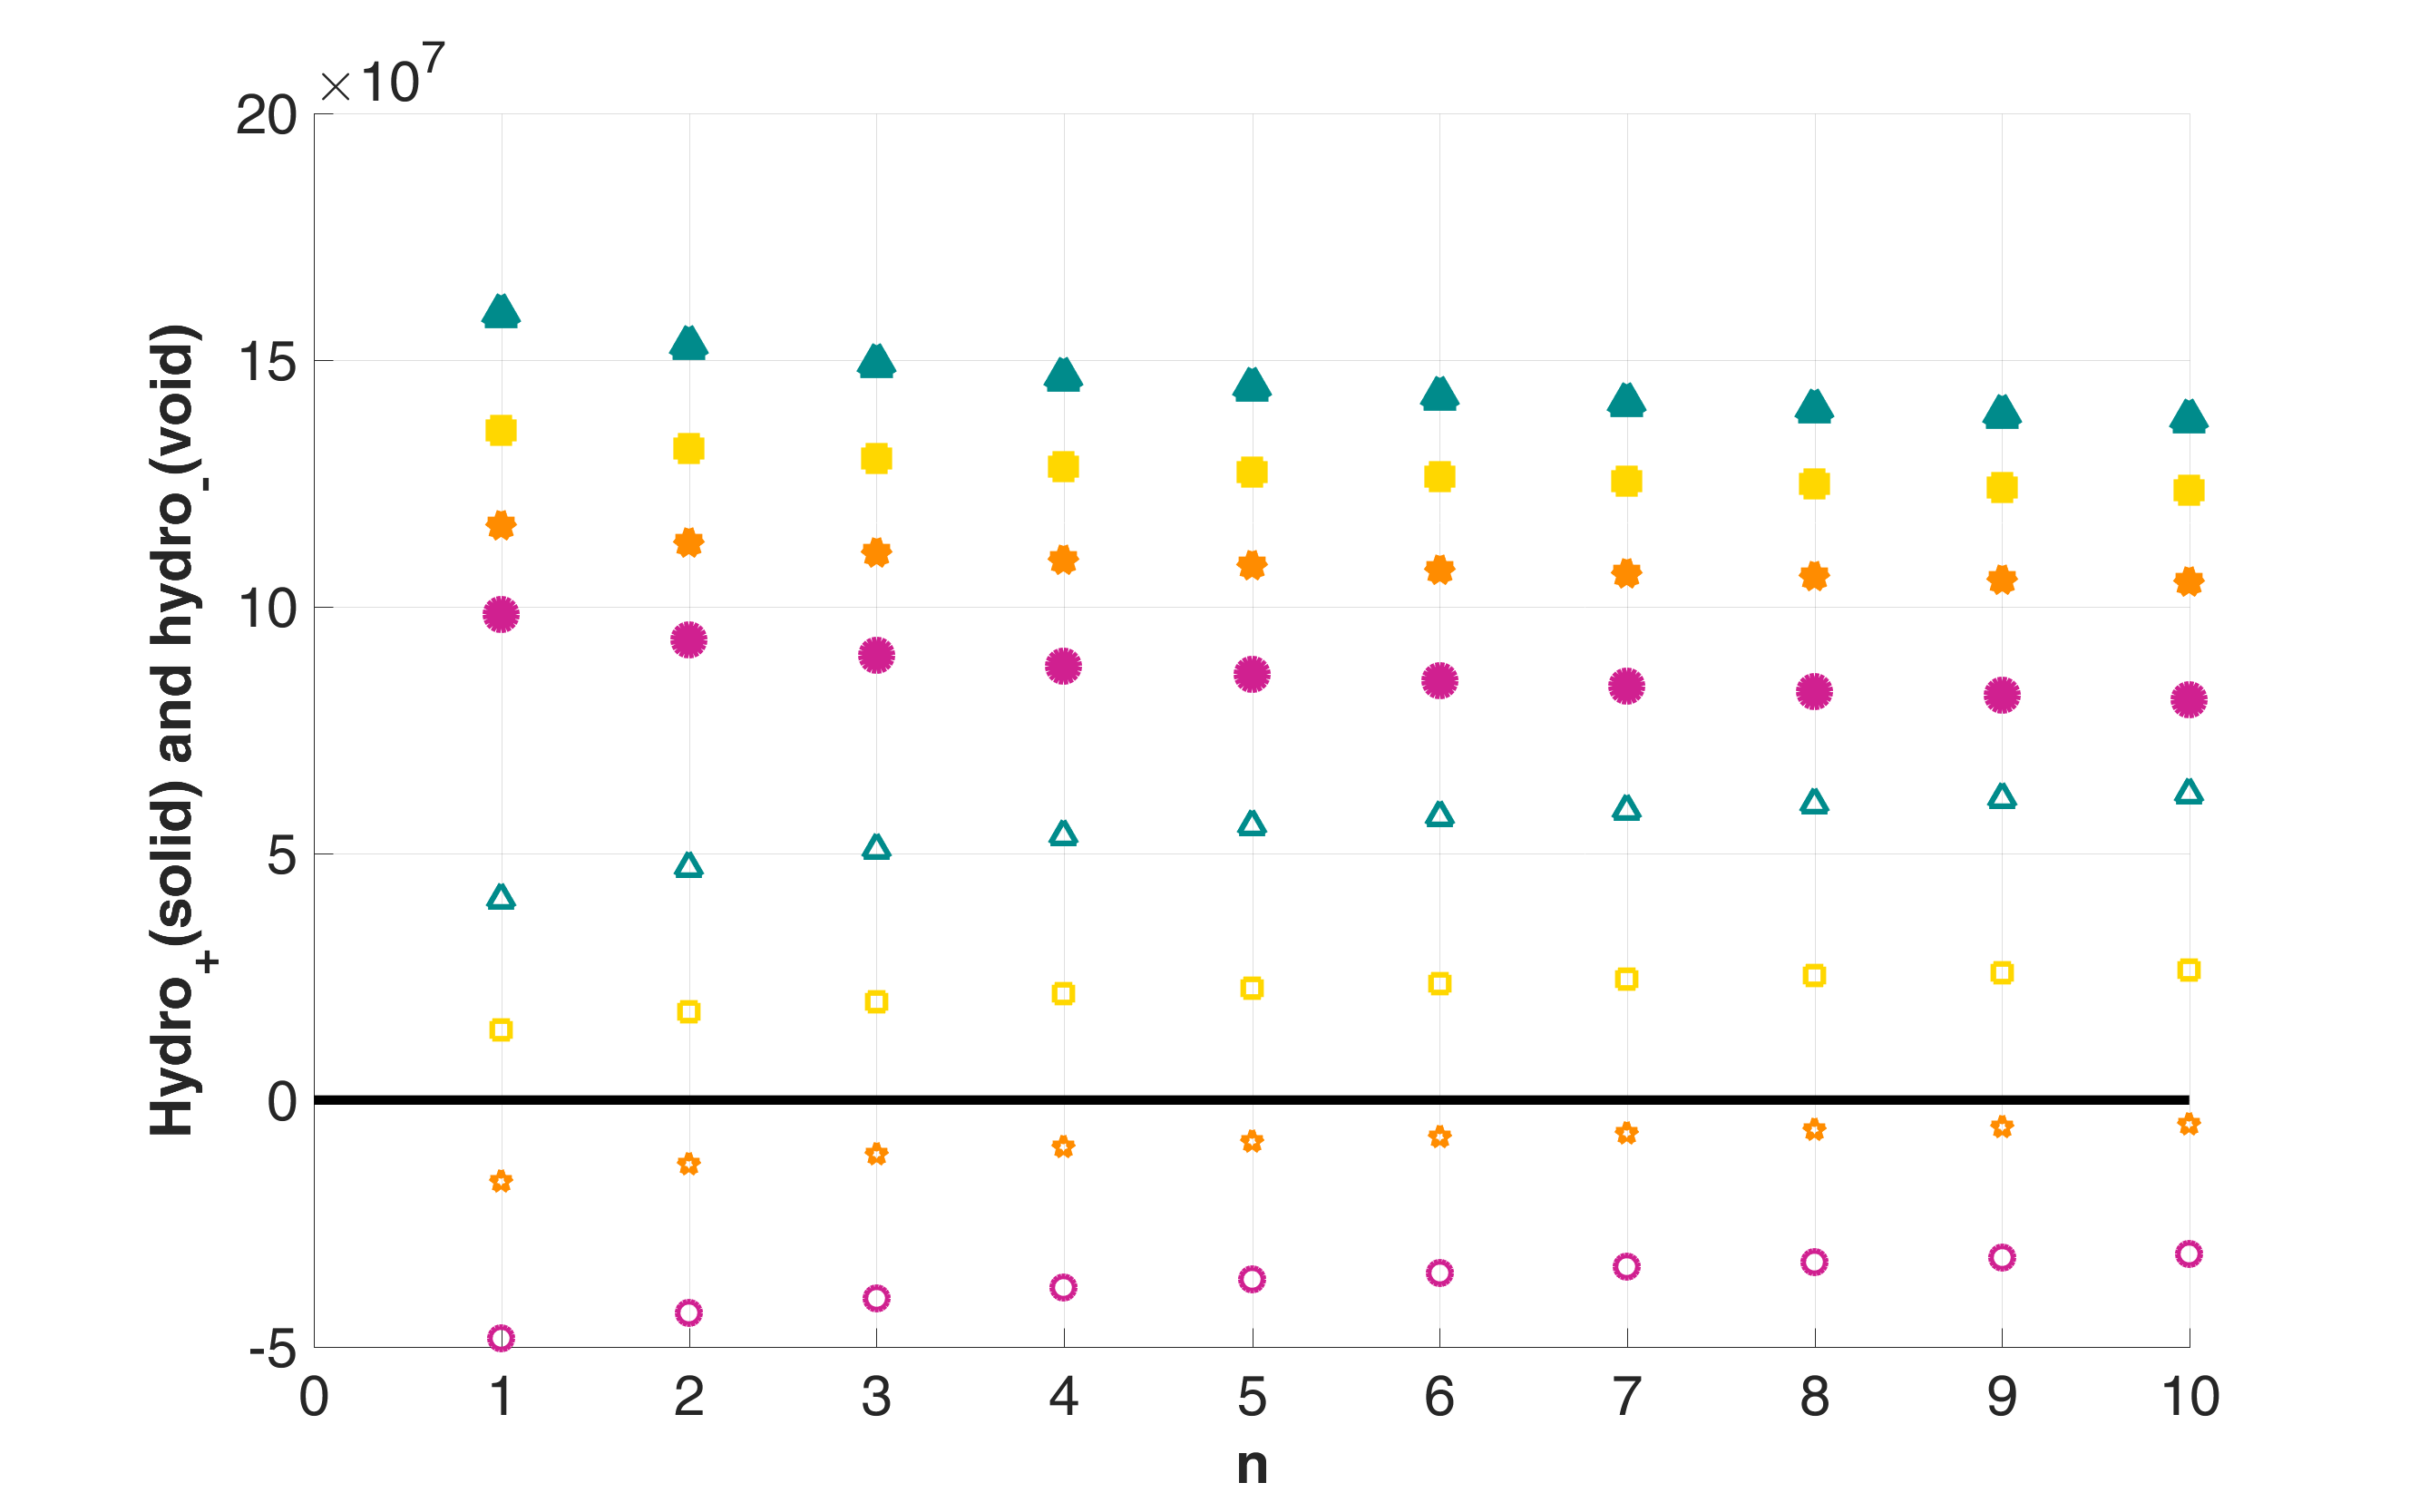
\includegraphics[width=\textwidth]{figures//10HNAP_b1D_m_hydro.png} 
	\caption{$Hydro_{+-}$ of bending tests with mean stress on 10HNAP}
	\label{fig.10HNAPhydro}
\end{figure}

In \figref{fig.10HNAP1} and \figref{fig.10HNAP2}, we give the prediction results of the torsion tests used to identify $\beta$ and $W_0$ of the model, then we use the bending with various mean stress to get the parameter $\lambda_+$. These are to be taken with caution because of the effect of the gradient because the specimens stressed in tension and in torsion are not of the same nature.
%%-------------S_eq vs NF----------------------------
\begin{figure}[!h]
	\centering
	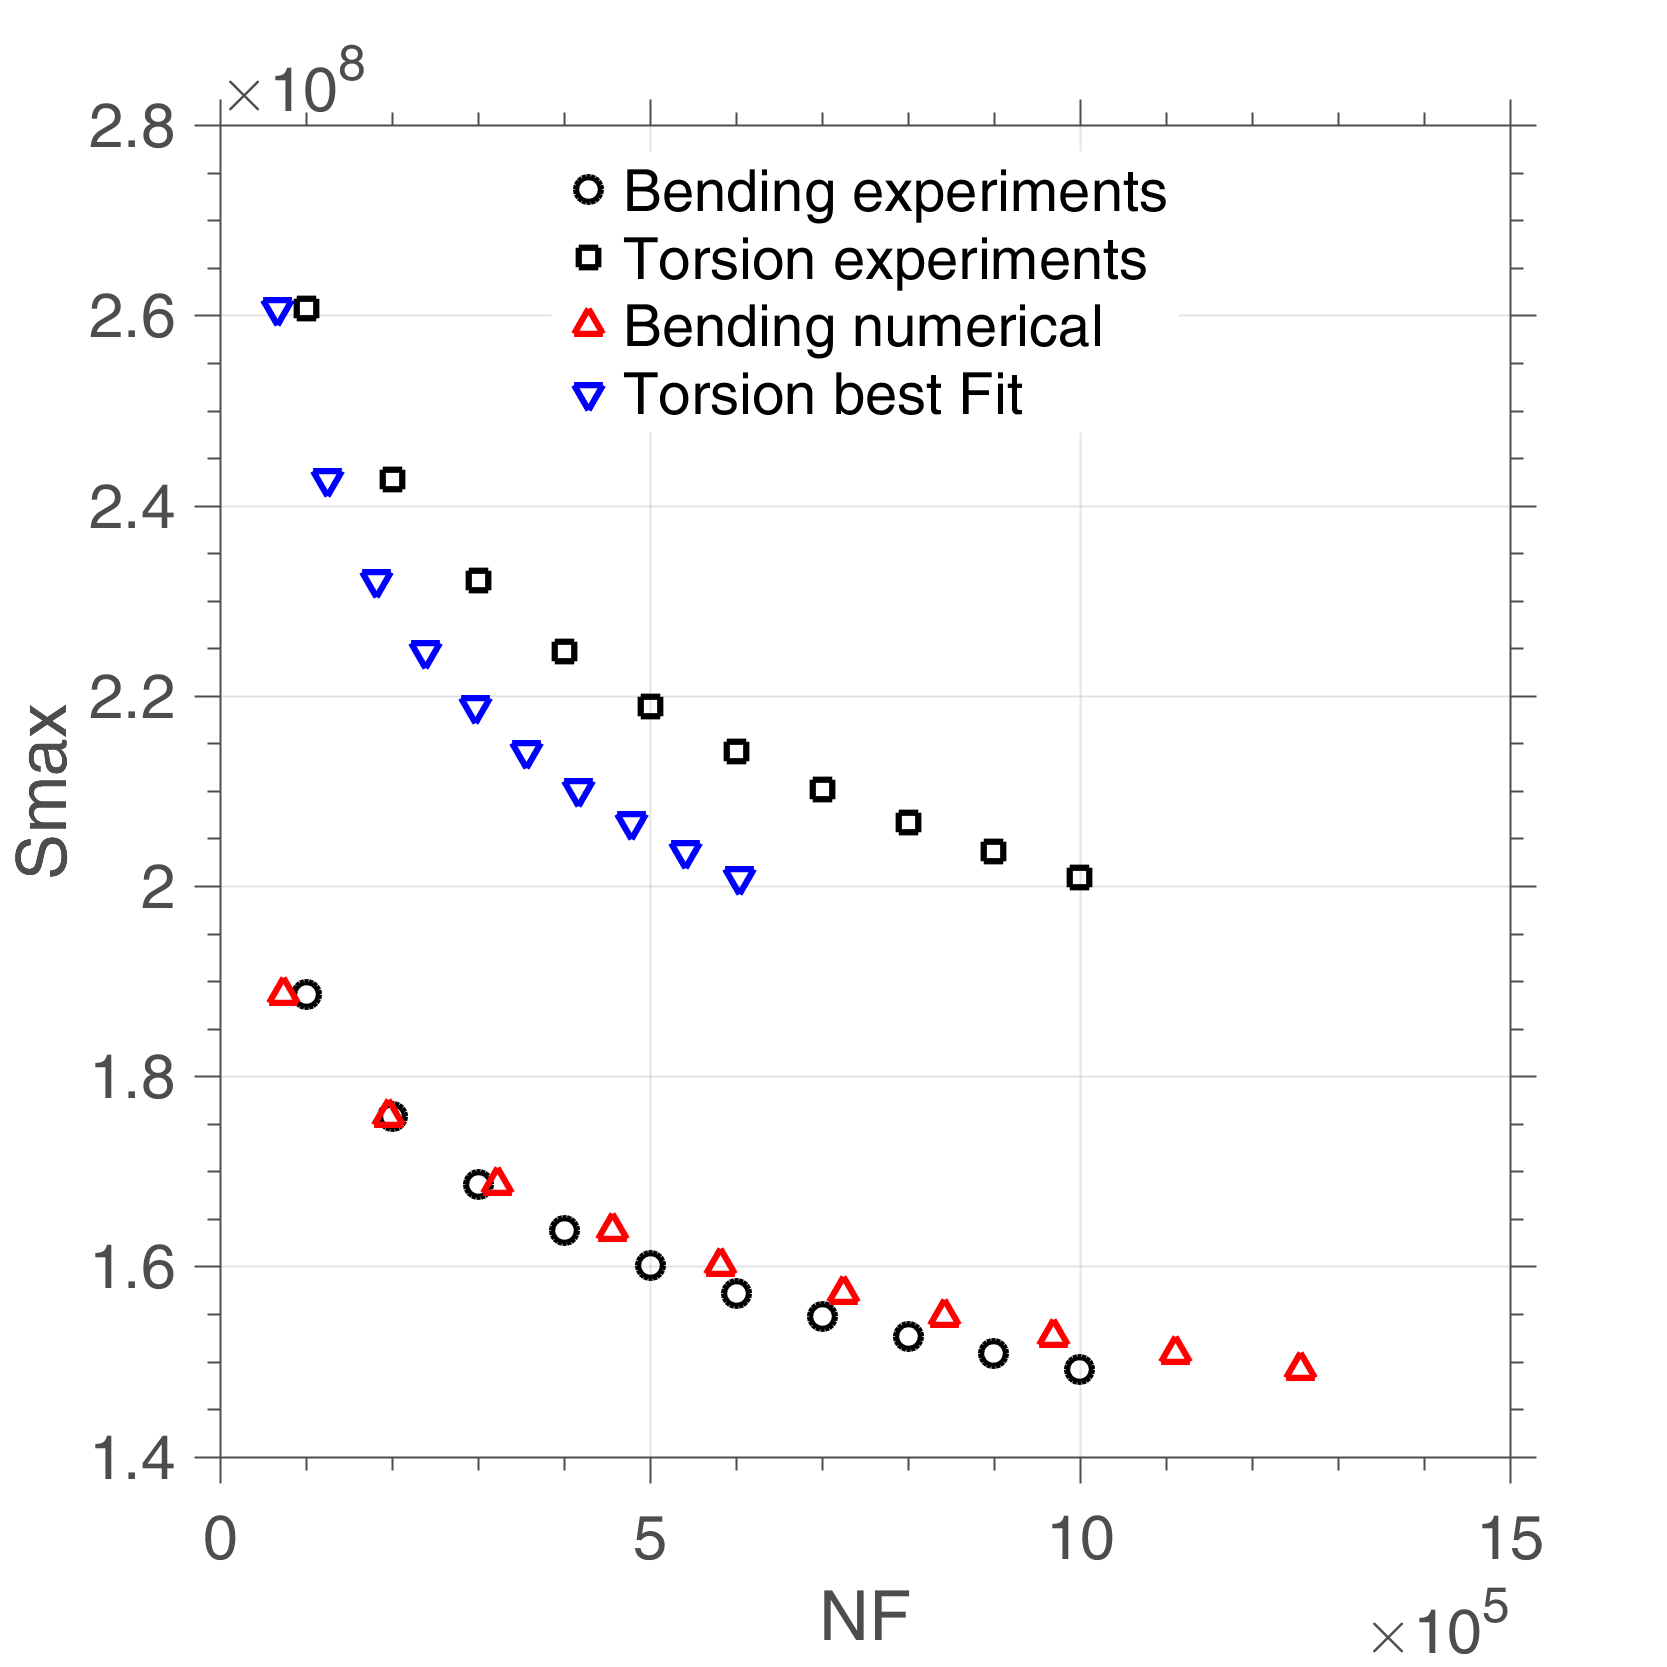
\includegraphics[width=\textwidth]{figures//10HNAP_bt1D_sn.png} 
	\caption{Bending and torsion test on 10HNAP steel(R=-1). Data are presented in Tab.\ref{tab.10HNAPbending} and  \ref{tab.10HNAPtorsion}. The torsion best fit and the bending numerical results(optimal time step of method 2 deduced in Chapter \ref{chp:5}) are obtained with the coefficients of Tab.\ref{tab.10HNAP.para}}
	\label{fig.bt1D10HNAPsn}
\end{figure}
\begin{figure}[!h]
	\centering
	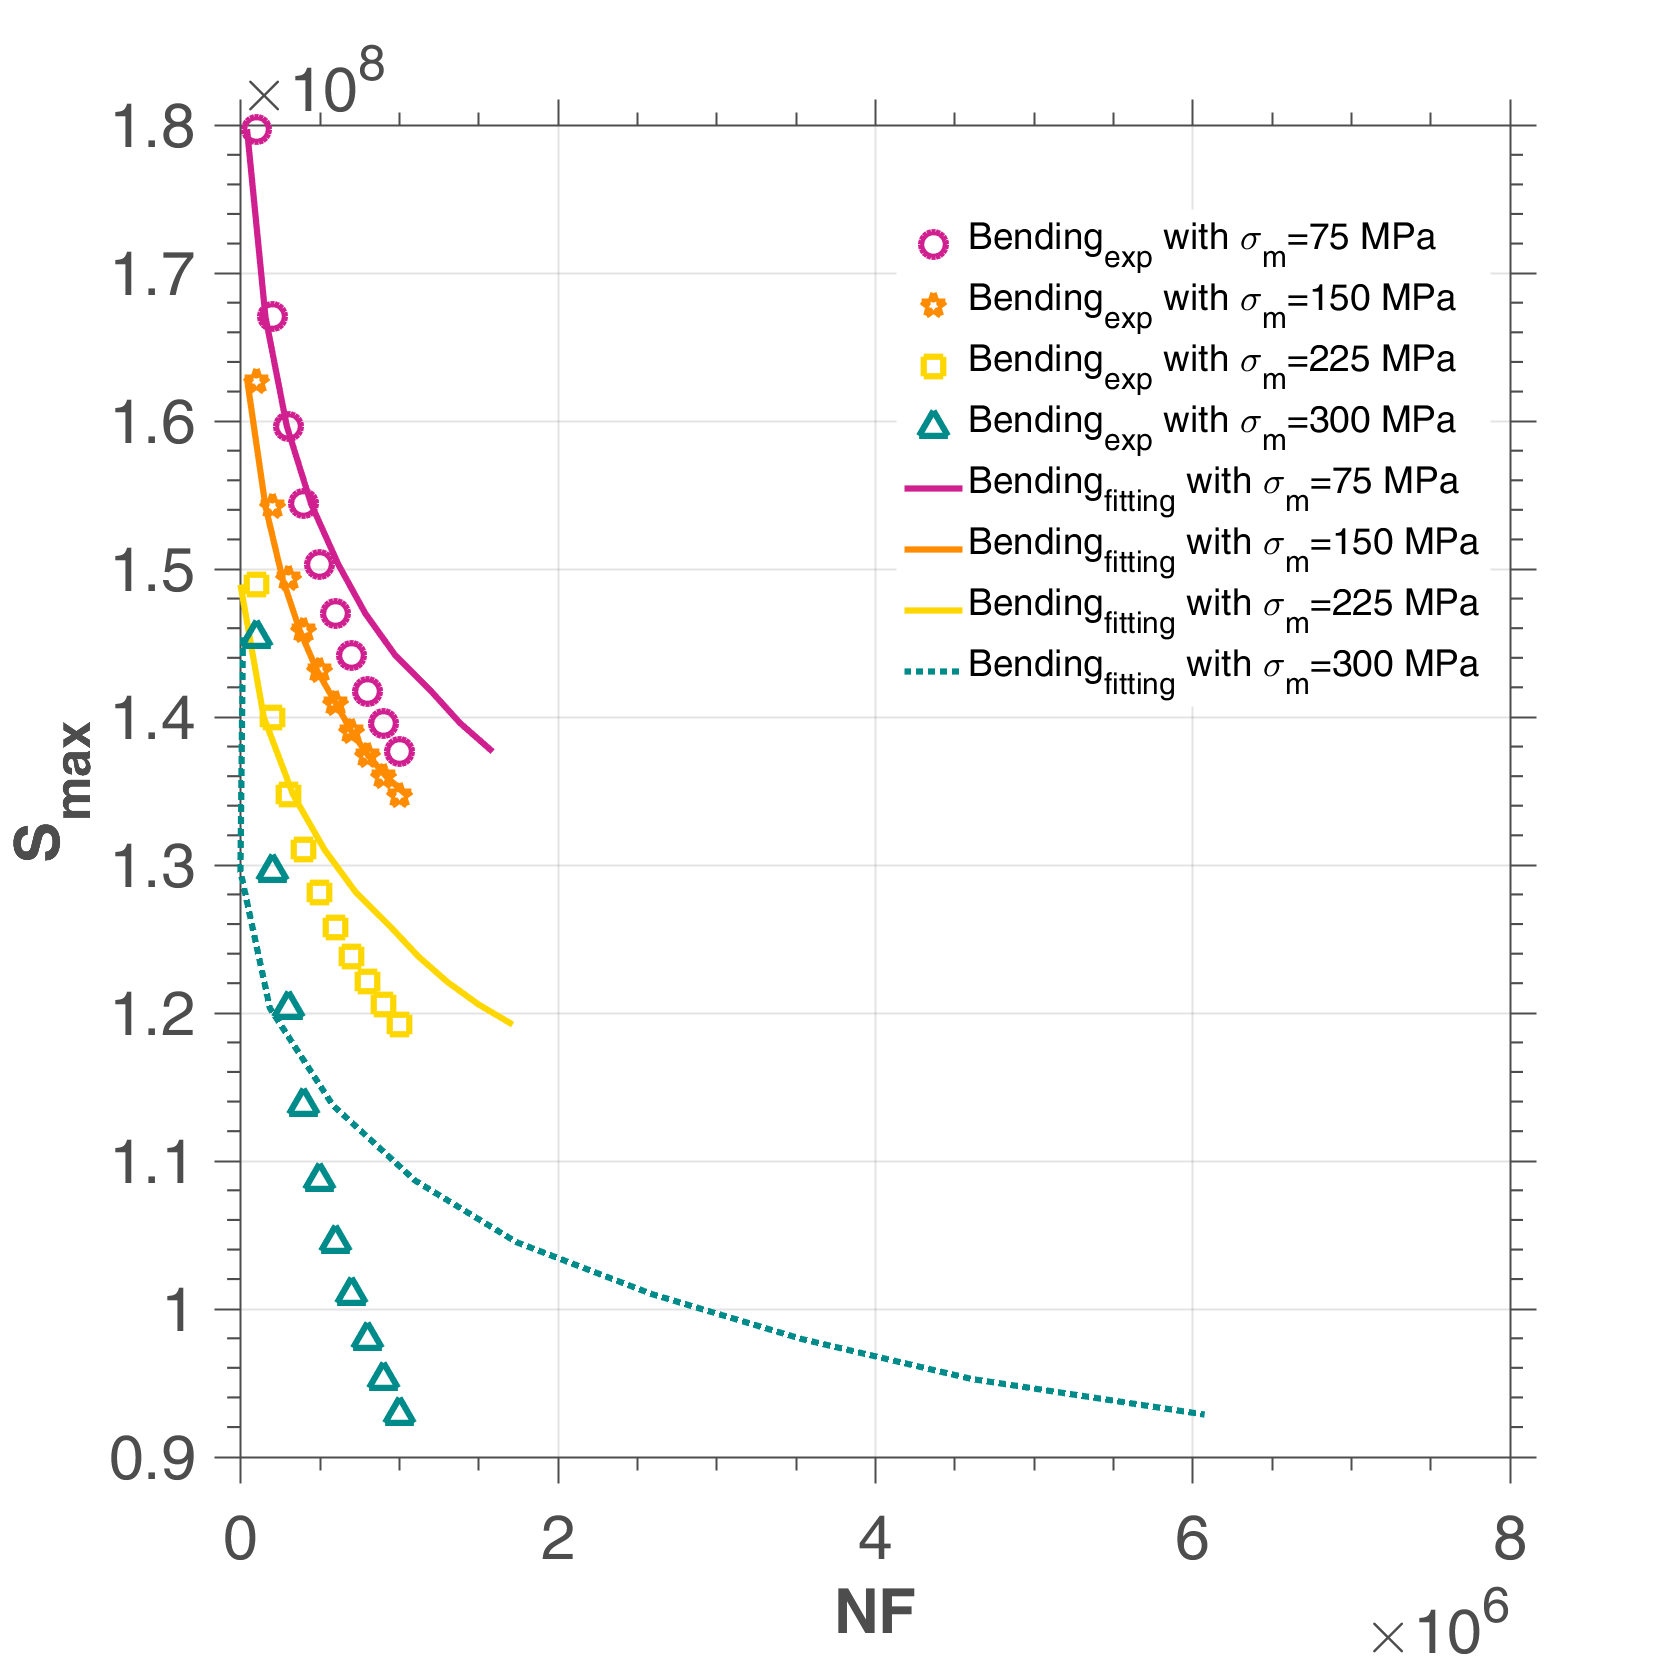
\includegraphics[width=\textwidth]{figures//10HNAP_b1D_m_sn.png} 
	\caption{Wöhler tensile curves for various mean stress values. Data are presented in Tab.\ref{tab.10HNAPmean} and results are obtained with the coefficients of Tab.\ref{tab.10HNAP.para}}
	\label{fig.b1Dm10HNAPsn}
\end{figure}


\begin{figure}[!h]
	\centering
	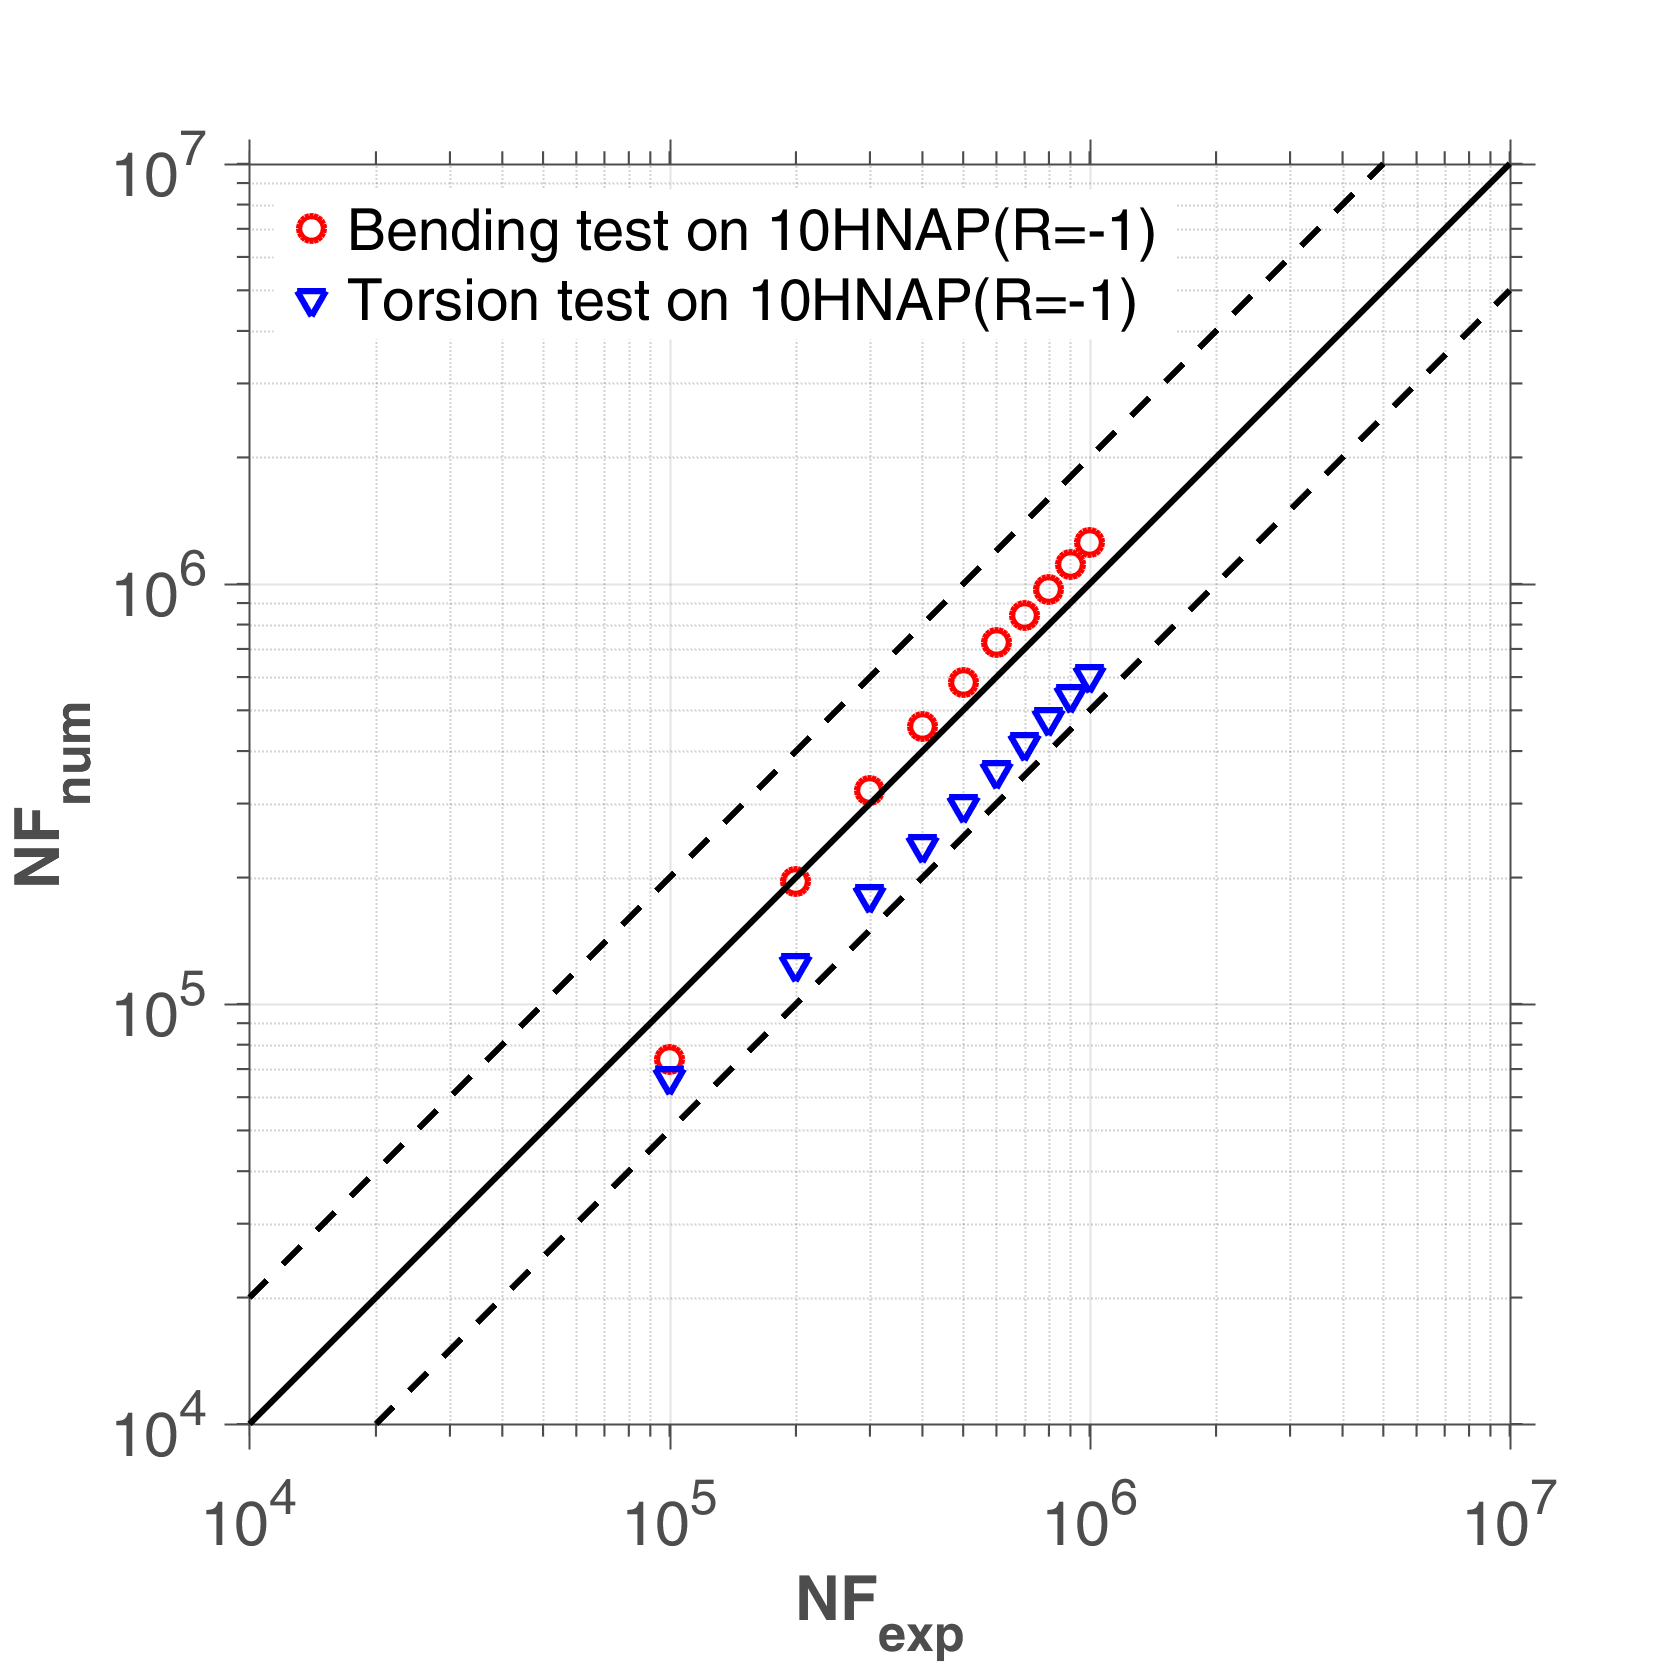
\includegraphics[width=\textwidth]{figures//10HNAP_bt1D_err.png} 
	\caption{Calibration on 10HNAP steel, bending and torsion tests on 10HNAP(R=-1). Data are presented in Tab.\ref{tab.10HNAPbending} and  \ref{tab.10HNAPtorsion} and results obtained with the coefficients of Tab.\ref{tab.10HNAP.para}}
	\label{fig.10HNAP1}
\end{figure}
\begin{figure}[!h]
	\centering
	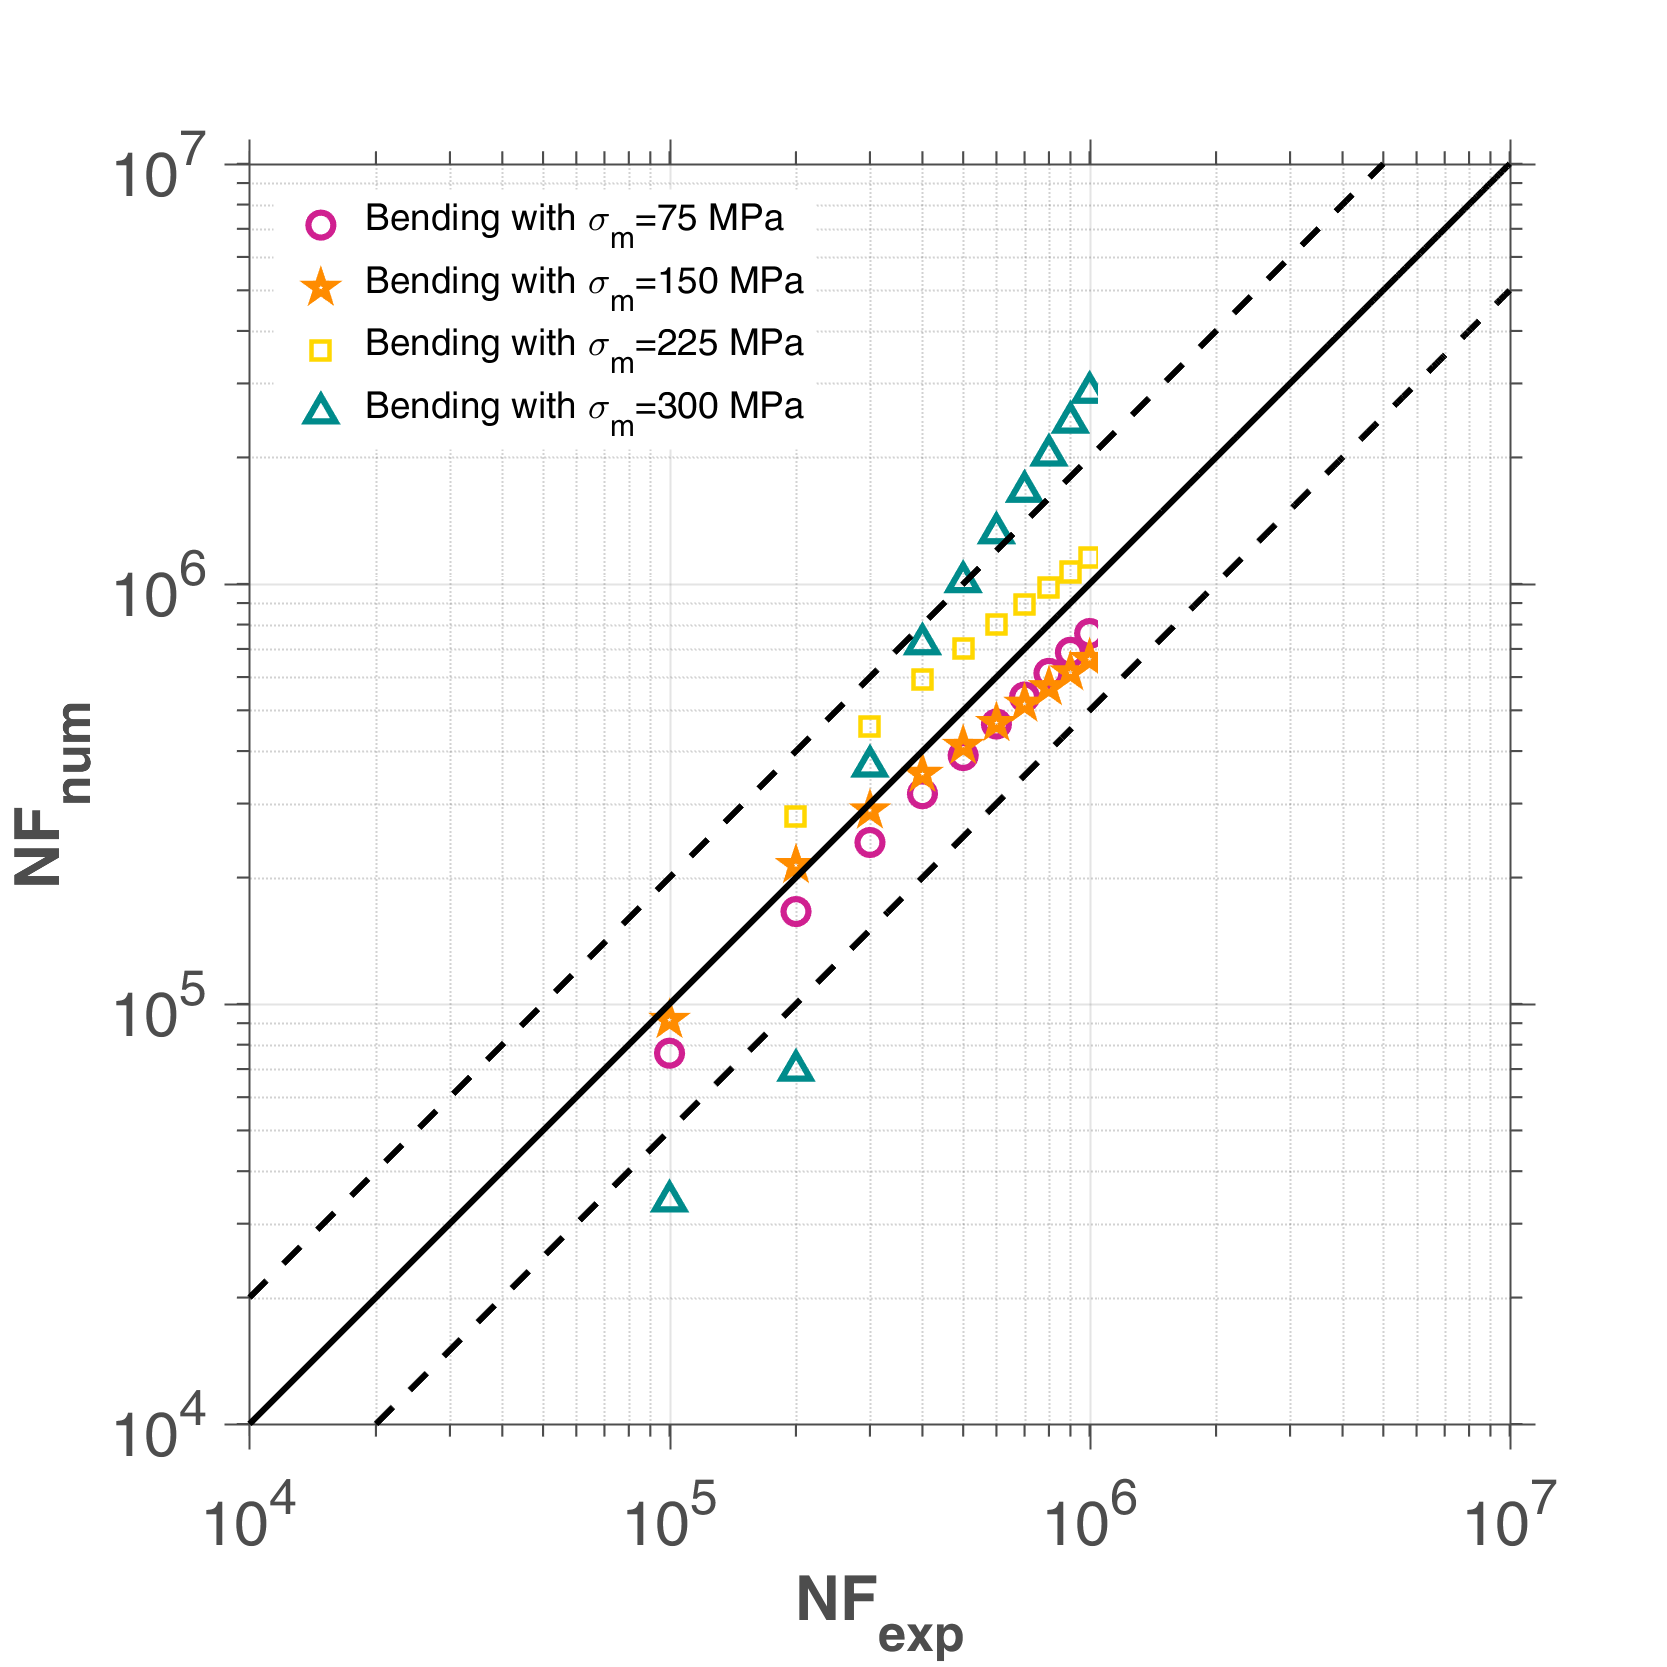
\includegraphics[width=\textwidth]{figures//10HNAP_b1D_m_err.png} 
	\caption{Calibration on 10HNAP steel, bending tests with various mean stress on 10HNAP, data from Tab.\ref{tab.10HNAPmean}  and results obtained with the coefficients of Tab.\ref{tab.10HNAP.para}}
	\label{fig.10HNAP2}
\end{figure}


The prediction results of the tensile tests for various values of the mean stress $\sigma_m$ are summarized in \figref{fig.10HNAP2}. These results correlate well with the experimental lifetimes. 


The tests of multiaxial loadings of variable amplitude are plotted in \figref{fig.10HNAP_random02} and \figref{fig.10HNAP_random05} as a function of the angle $\alpha_{M}$ and the ratio $r$. In these figures, the prediction results of the proposed model and that presented by \cite{carpinteri2003multiaxial}. For the first type of tests ($\alpha_{M} = \pi/8$ and r = 0.2), and the second type of tests ($\alpha_{M} = \pi/4$ and r = 0.5), the predictions of \cite{carpinteri2003multiaxial} are both good. 
\begin{figure}[!h]
	\centering
	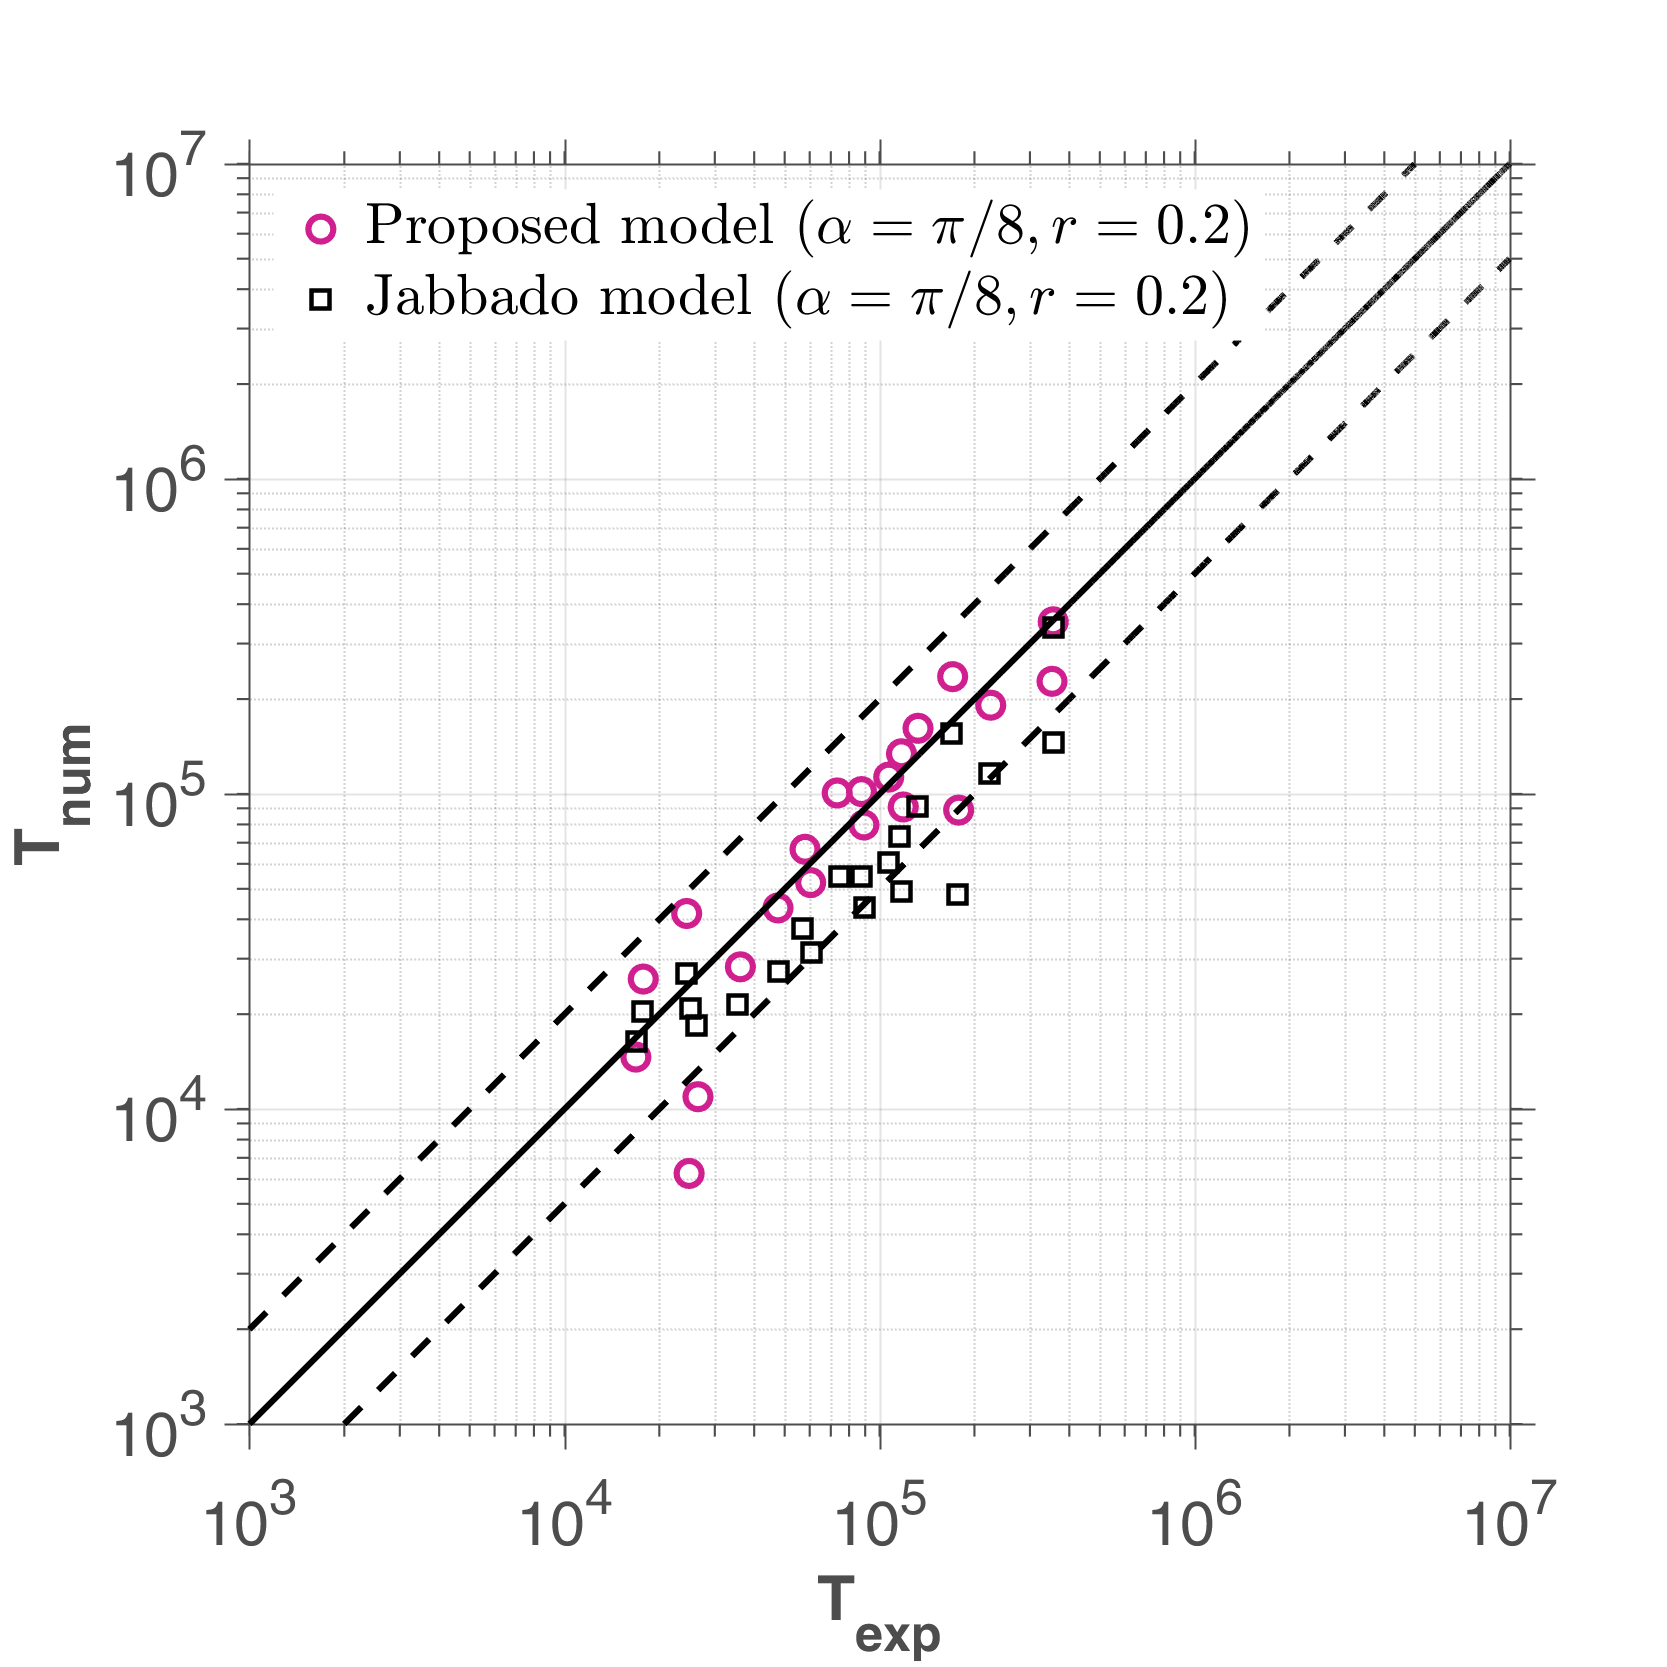
\includegraphics[width=\textwidth]{figures//HNAP_random_r02_error.png} 
	\caption{Random bending-torsion 2D tests on 10HNAP, data from Tab.\ref{tab.10HNAPrand1} and \cite{jabbado:pastel-00002116}. Results are obtained with the coefficients of Tab.\ref{tab.10HNAP.para.random} ($\alpha_{M} = \pi/8$ and r = 0.2)}
	\label{fig.10HNAP_random02}
\end{figure}

\begin{figure}[!h]
	\centering
	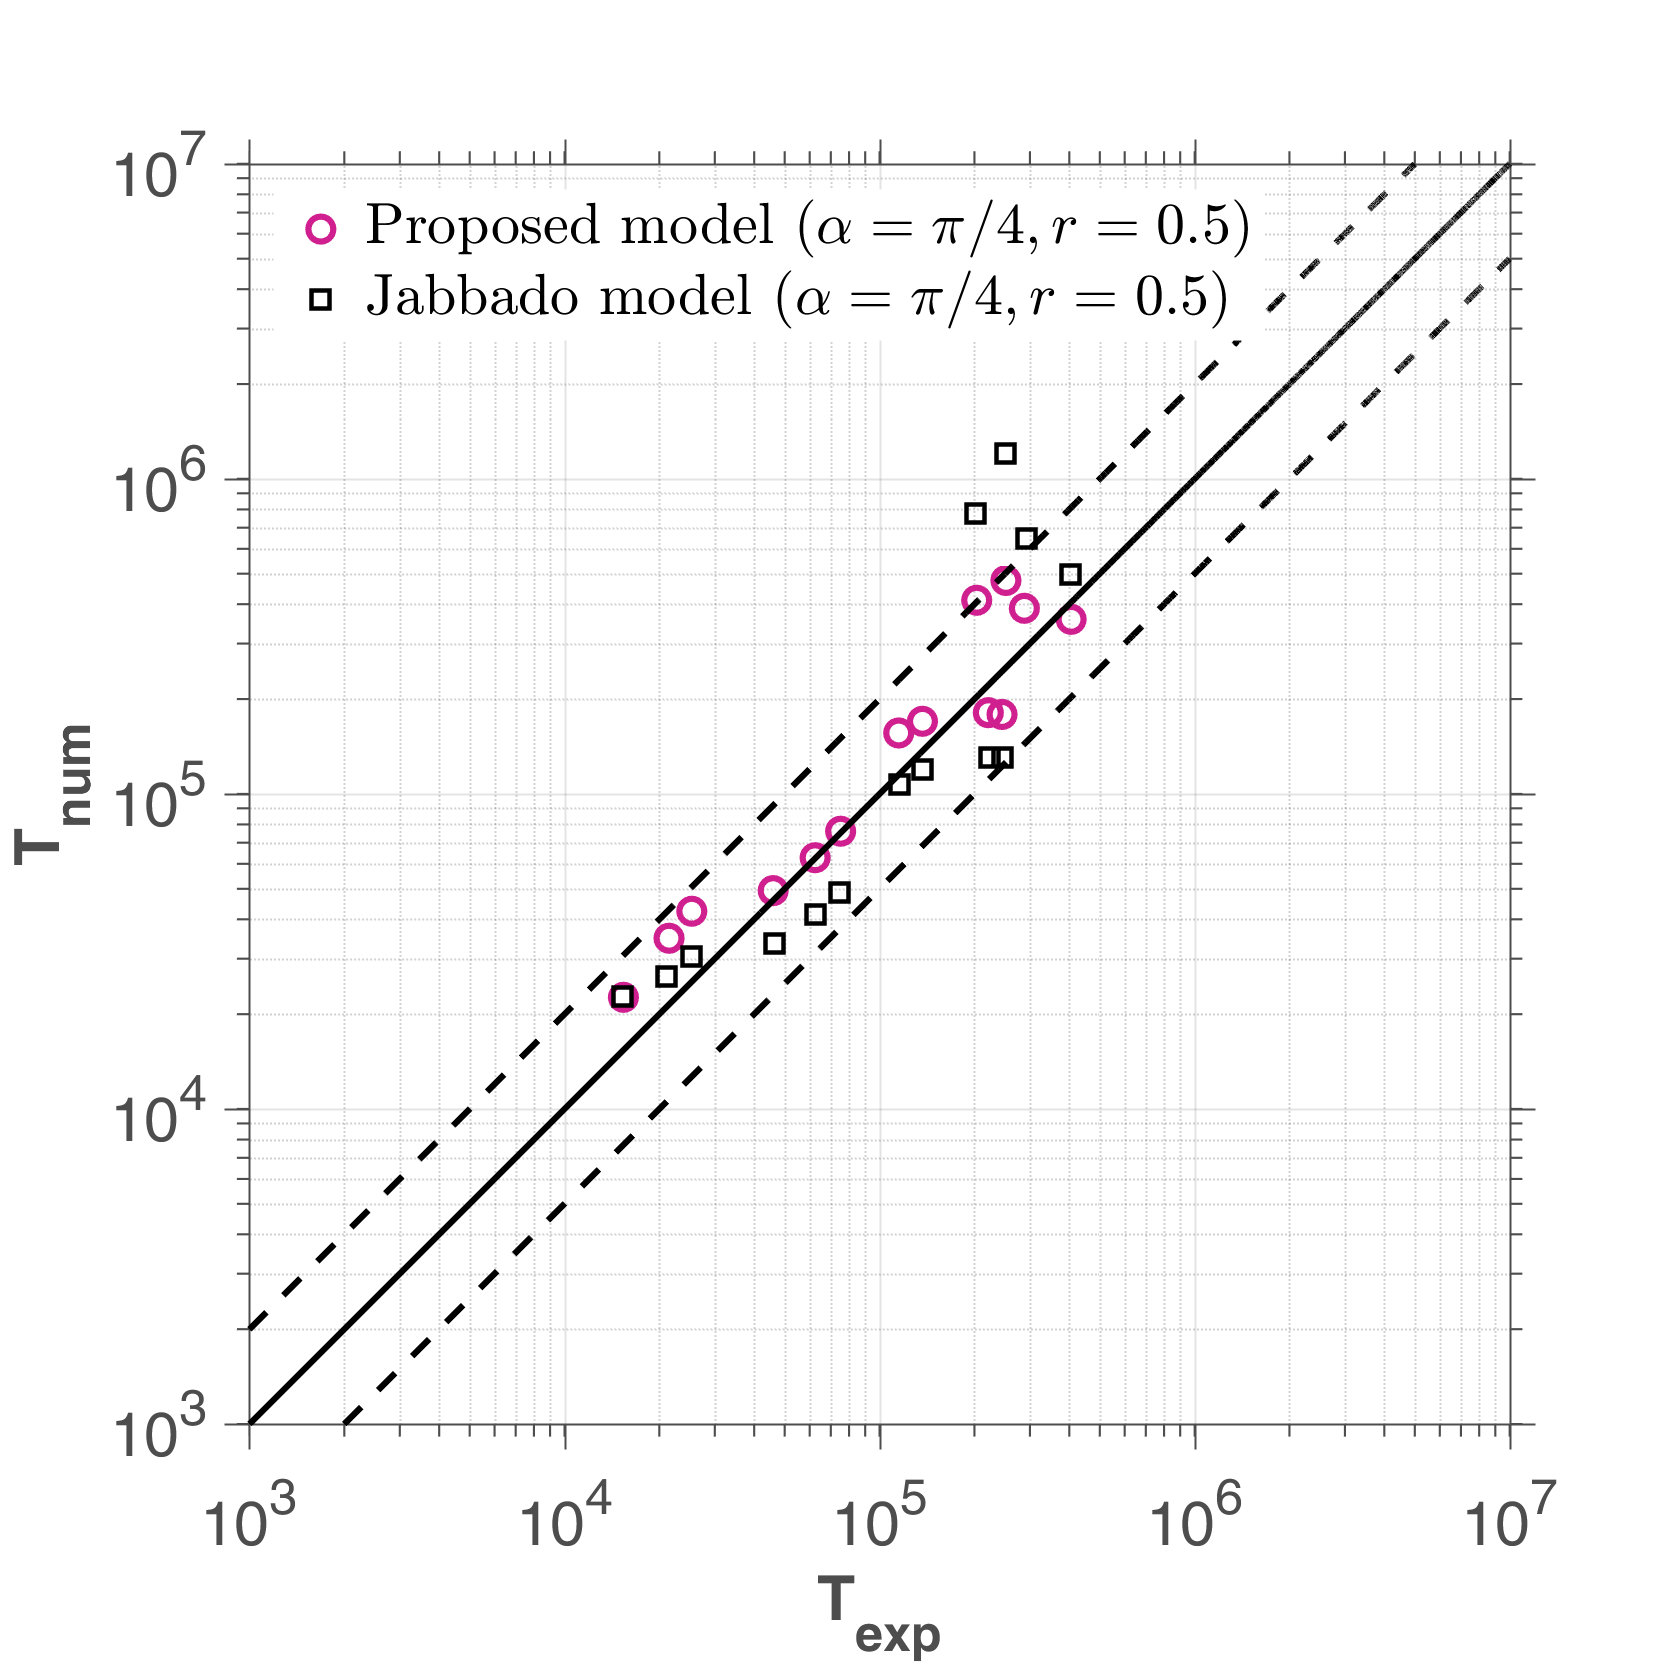
\includegraphics[width=\textwidth]{figures//HNAP_random_r05_error.png} 
	\caption{Random bending-torsion 2D tests on 10HNAP, data from Tab.\ref{tab.10HNAPrand2} and \cite{jabbado:pastel-00002116}. Results are obtained with the coefficients of Tab.\ref{tab.10HNAP.para.random} ($\alpha_{M} = \pi/4$ and r = 0.5)}
	\label{fig.10HNAP_random05}
\end{figure}


\clearpage
\section{Conclusions}

We work on the stress tensor directly in 3D analysis in stead of using the multidimensional equivalent stress.
The strategy can be made more complex by introducing a local space averaging process in the calculation of the local damage, and by taking more general plastic flows. The energy based fatigue approach takes into account impurities and hardness in the material and is applicable to any type of micro plasticity law and multiaxial load geometry. The time implicit strategy gets rid of cycle counting which is hardly applicable to complex loading, big fluctuation is magnified which reflects the real situation.

There are several advantages and drawbacks of our proposed model. The time implicit method does not take the unit of cycle so as to avoid cycle counting and relevant methods such as rain-flow filter. The possibility to handle different S-N curves corresponding to various materials and load conditions via changing the parameters. We also have the random loading suitability with nonlinear damage accumulation. The drawback is this strategy requires a scale by scale analysis which can be complicated for very high cycle fatigue. However, as introduced above, we can use the optimal time step method to calculate precisely the representative loading history sequence and use scalar integration for the rest of fatigue life. In this way the numerical cost can be dramatically reduced without losing the precision.

Since our method is based on the Dang Van paradigm, to deal with mean stress effect and multiaxial loads we only have the parameter $\lambda_{+-}$, which is insufficient to fit the experiments. In fact, our microplasticity model is probably too crude to handle situations where there is  a clear strain path effect.

Also, we need more experimental data and comparison with other results form the literature.



\vspace{6pt}
\noindent
\textbf{Acknowledgments}

\vspace{6pt}
We are grateful for the financial and technical support of Chaire PSA.

\bibliographystyle{unsrt}
\bibliography{11}
\addcontentsline{toc}{section}{Reference}



%\clearpage
%\appendix
%\appendixpage
%\addcontentsline{toc}{section}{Appendices}\markboth{APPENDICES}{}
%\lstset{% general command to set parameter(s)
%basicstyle=\small,  
%keywordstyle=\color{red},  
%identifierstyle=, % nothing happens
%commentstyle=\color{blue},
%stringstyle=\ttfamily, % typewriter type for strings
%showstringspaces=false} % no special string spaces
%	\section{DETAILED EXPLOITATION}
%	************************************************************************************

 A DETAILED DESCRIPTION OF ANALYTICAL EXPLOITATION ON UNIAXIAL CYCLE
 
\noindent              
************************************************************************************

\noindent
\textbf{Phase 1:} The deviatoric stress amplitude increases from $\sigma_y/s$ to $S_{max}$.

\noindent
The material is in local plastic regime, then $\dot{\varepsilon}^p>0$ and $\dot{\sigma}-\dot{b}=0$ $\Rightarrow$ $\dot{\Sigma}-\dfrac{E}{1+\nu}\dot{\varepsilon}^p=\dfrac{kE}{E-k}\dot{\varepsilon}^p$ $\Rightarrow$ 
$$\dot{\varepsilon}^p=\dfrac{(E- k)(1+\nu)}{E(E+k\nu)}\dot{\Sigma}.$$

\vspace{6pt}
\noindent
$\Rightarrow$ $\dot{\varepsilon}^p$ varies from 0 to $\dfrac{(E- k)(1+\nu)(S_{max}-\sigma_y/s)}{E(E+k\nu)}$.

\vspace{6pt}
\noindent
From Taylor-Lin scale transition model:
$$\dot{\sigma}=\dot{\Sigma}-\dfrac{E}{1+\nu}\dot{\varepsilon}_p=\dot{\Sigma}-\dfrac{E-k}{E-\nu k}\dot{\Sigma}=\dfrac{k(1-\nu)}{E-k\nu}\dot{\Sigma}.$$

\vspace{6pt}
\noindent
$\Rightarrow$ $\sigma$ varies from $\sigma_y/s$ to $\sigma_y/s+\dfrac{k(1-\nu)(S_{max}-\sigma_y/s)}{E-k\nu}$.

\vspace{6pt}
$$\dot{b}=\dot{\Sigma}-\dfrac{E}{1+\nu}\dot{\varepsilon}_p=\dot{\Sigma}-\dfrac{E-k}{E-\nu k}\dot{\Sigma}=\dfrac{k(1-\nu)}{E-k\nu}\dot{\Sigma}.$$

\vspace{6pt}
\noindent
$\Rightarrow$ $b$ varies from $0$ to $\dfrac{k(1-\nu)(S_{max}-\sigma_y/s)}{E-k\nu}$.

\vspace{6pt}
\noindent
So the energy dissipation rate is: $$(\sigma-b)\dot{\varepsilon}^p=\dfrac{\sigma_y}{s}\dot{\varepsilon}^p=\dfrac{\sigma_y}{s}\dfrac{(E- k)(1+\nu)}{E(E+k\nu)}\dot{\Sigma}.$$

\noindent
The energy dissipation is: $$(\sigma-b)\Delta\varepsilon^p=\dfrac{\sigma_y}{s}\dfrac{(E- k)(1+\nu)(S_{max}-\sigma_y/s)}{E(E+k\nu)}.$$

\vspace{6pt}
\noindent
\textbf{Phase 2:} The deviatoric stress amplitude decreases from $S_{max}$ to $S_{max}-2\sigma_y/s$.

\noindent
The material is in local elastic regime, then $\dot{\varepsilon}^p=0$ and $\dot{\sigma}-\dot{b}=0$ $\Rightarrow$

\vspace{6pt}
\noindent
$\dot{b}=0$, $\dot{\sigma}=\dot{\Sigma}-\dfrac{E}{1+\nu}\dot{\varepsilon}_p=\dot{\Sigma}$.

\vspace{6pt}
\noindent
$\sigma$ varies from $\sigma_y/s+\dfrac{k(1-\nu)(S_{max}-\sigma_y/s)}{E-k\nu}$ to $-\sigma_y/s+\dfrac{k(1-\nu)(S_{max}-\sigma_y/s)}{E-k\nu}$.

\vspace{6pt}
\noindent
$\sigma-b$ varies from $\sigma_y/s$ to $-\sigma_y/s$.

\vspace{6pt}
\noindent
The energy dissipation rate is: $$(\sigma-b)\dot{\varepsilon}^p=0.$$

\vspace{6pt}
\noindent
\textbf{Phase 3:} The deviatoric stress amplitude decreases from $S_{max}-2\sigma_y/s$ to $-S_{max}$.

\noindent
The material is in local plastic regime, then $\dot{\varepsilon}^p>0$ and $\dot{\sigma}-\dot{b}=0$ $\Rightarrow$ 
$$\dot{\varepsilon}^p=\dfrac{(E- k)(1+\nu)}{E(E+k\nu)}\dot{\Sigma}$$ as opposite to phase 1 for $\dot{\Sigma}<0$.

\vspace{6pt}
\noindent
$\Rightarrow$ $\varepsilon^p$ varies from $\dfrac{(E- k)(1+\nu)(S_{max}-\sigma_y/s)}{E(E+k\nu)}$ to 

\noindent
$\dfrac{(E- k)(1+\nu)(S_{max}-\sigma_y/s-S_{max}-(S_{max}-2\sigma_y/s))}{E(E+k\nu)}=-\dfrac{(E- k)(1+\nu)(S_{max}-\sigma_y/s)}{E(E+k\nu)}$.

\vspace{6pt}
\noindent
From Taylor-Lin scale transition model:
$$\dot{\sigma}=\dot{\Sigma}-\dfrac{E}{1+\nu}\dot{\varepsilon}_p=\dot{\Sigma}-\dfrac{E-k}{E-\nu k}\dot{\Sigma}=\dfrac{k(1-\nu)}{E-k\nu}\dot{\Sigma}.$$

\vspace{6pt}
\noindent
$\Rightarrow$ $\sigma$ varies from $-\sigma_y/s+\dfrac{k(1-\nu)(S_{max}-\sigma_y/s)}{E-k\nu}$ to $-\sigma_y/s-\dfrac{k(1-\nu)(S_{max}-\sigma_y/s)}{E-k\nu}$.

\vspace{6pt}
$$\dot{b}=\dot{\Sigma}-\dfrac{E}{1+\nu}\dot{\varepsilon}_p=\dot{\Sigma}-\dfrac{E-k}{E-\nu k}\dot{\Sigma}=\dfrac{k(1-\nu)}{E-k\nu}\dot{\Sigma}.$$
\vspace{6pt}
\noindent
$\Rightarrow$ $b$ varies from $\dfrac{k(1-\nu)(S_{max}-\sigma_y/s)}{E-k\nu}$ to $-\dfrac{k(1-\nu)(S_{max}-\sigma_y/s)}{E-k\nu}$.

\vspace{6pt}
\noindent
So the energy dissipation rate is: $$(\sigma-b)\dot{\varepsilon}^p=-\dfrac{\sigma_y}{s}\dot{\varepsilon}^p=-\dfrac{\sigma_y}{s}\dfrac{(E- k)(1+\nu)}{E(E+k\nu)}\dot{\Sigma}.$$

\noindent
The energy dissipation is: $$(\sigma-b)\Delta\varepsilon^p=-\dfrac{\sigma_y}{s}\dfrac{(E- k)(1+\nu)(-2S_{max}+2\sigma_y/s)}{E(E+k\nu)}=\dfrac{2\sigma_y}{s}\dfrac{(E- k)(1+\nu)(S_{max}-\sigma_y/s)}{E(E+k\nu)}.$$



\vspace{6pt}
\noindent
\textbf{Phase 4:} The deviatoric stress amplitude increases from $-S_{max}$ to $-S_{max}+2\sigma_y/s$.

\noindent
The material is in local elastic regime, then $\dot{\varepsilon}^p=0$ and $\dot{\sigma}-\dot{b}=0$ $\Rightarrow$

\vspace{6pt}
\noindent
$\dot{b}=0$, $\dot{\sigma}=\dot{\Sigma}-\dfrac{E}{1+\nu}\dot{\varepsilon}_p=\dot{\Sigma}$.

\vspace{6pt}
\noindent
$\sigma$ varies from $-\sigma_y/s-\dfrac{k(1-\nu)(S_{max}-\sigma_y/s)}{E-k\nu}$ to $\sigma_y/s-\dfrac{k(1-\nu)(S_{max}-\sigma_y/s)}{E-k\nu}$.

\vspace{6pt}
\noindent
$\sigma-b$ varies from $-\sigma_y/s$ to $\sigma_y/s$.

\vspace{6pt}
\noindent
So the energy dissipation rate is: $$(\sigma-b)\dot{\varepsilon}^p=0.$$


\vspace{6pt}
\noindent
\textbf{Phase 5:} The deviatoric stress amplitude increases from $-S_{max}+2\sigma_y/s$ to $\sigma_y/s$.

\noindent
The material is in local plastic regime, then $\dot{\varepsilon}^p>0$ and $\dot{\sigma}-\dot{b}=0$ $\Rightarrow$ 
$$\dot{\varepsilon}^p=\dfrac{(E- k)(1+\nu)}{E(E+k\nu)}\dot{\Sigma}$$ as in phase 1.

\vspace{6pt}
\noindent
$\Rightarrow$ $\dot{\varepsilon}^p$ varies from $-\dfrac{(E- k)(1+\nu)(S_{max}-\sigma_y/s)}{E(E+k\nu)}$ to $0$.

\vspace{6pt}
$$\dot{\sigma}=\dot{\Sigma}-\dfrac{E}{1+\nu}\dot{\varepsilon}_p=\dot{\Sigma}-\dfrac{E-k}{E-\nu k}\dot{\Sigma}=\dfrac{k(1-\nu)}{E-k\nu}\dot{\Sigma}.$$

\vspace{6pt}
\noindent
$\Rightarrow$ $\sigma$ varies from $\sigma_y/s-\dfrac{k(1-\nu)(S_{max}-\sigma_y/s)}{E-k\nu}$ to $\sigma_y/s$.

\vspace{6pt}
$$\dot{b}=\dot{\Sigma}-\dfrac{E}{1+\nu}\dot{\varepsilon}_p=\dot{\Sigma}-\dfrac{E-k}{E-\nu k}\dot{\Sigma}=\dfrac{k(1-\nu)}{E-k\nu}\dot{\Sigma}.$$
\vspace{6pt}
\noindent
$\Rightarrow$ $b$ varies from $-\dfrac{k(1-\nu)(S_{max}-\sigma_y/s)}{E-k\nu}$ to $0$.

\vspace{6pt}
\noindent
So the energy dissipation rate is: $$(\sigma-b)\dot{\varepsilon}^p=\dfrac{\sigma_y}{s}\dot{\varepsilon}^p=\dfrac{\sigma_y}{s}\dfrac{(E- k)(1+\nu)}{E(E+k\nu)}\dot{\Sigma}.$$

\noindent
The energy dissipation is: $$(\sigma-b)\Delta\varepsilon^p=\dfrac{\sigma_y}{s}\dfrac{(E- k)(1+\nu)(S_{max}-\sigma_y/s)}{E(E+k\nu)}.$$


From the three phase analysis in local plastic regime, the dissipated energy is like $dW(phase1)=\dfrac{1}{2}dW(phase3)=dW(phase5)$ and the dissipation rate is like $d\dot{W}(phase1)=d\dot{W}(phase3)=d\dot{W}(phase5)$.
\begin{equation}d\dot{W}=\dfrac{(E-k)(1+\nu) }{E(E-k\nu)}\left( \dfrac{\sigma_y}{s}\right) \left| \dot{\Sigma}\right|   
\end{equation}


%	\clearpage
************************************************************************************

MULTI-DIMENSIONAL PLASTIC AND ELASTIC REGIME ANALYSIS

************************************************************************************

At a certain scale $s_i$, after elimination of $ \dot{\uline{\uline{\varepsilon}}}^p$, there are 
$$\dot{\uline{\uline{S}}}- \dot{\uline{\uline{b}}}= dev\dot{\uline{\uline{\Sigma}}}-E\gamma\left( \dfrac{1}{1+\nu}+\dfrac{k}{E-k}\right)\dfrac{\uline{\uline{S}}-\uline{\uline{b}}}{\left| \left|\uline{\uline{S}}-\uline{\uline{b}}\right| \right|}. $$

If we are at yield limit at (t+dt), we get on the other hand:
$$\left( \uline{\uline{S}}-\uline{\uline{b}}\right) (t+dt)=\left( \uline{\uline{S}}-\uline{\uline{b}}\right) (t)+\left( \dot{\uline{\uline{S}}}- \dot{\uline{\uline{b}}}\right) dt,$$
\begin{equation}\left| \left| \left( \uline{\uline{S}}-\uline{\uline{b}}\right) (t+dt)\right| \right| =\left( \sigma_y-\lambda \sigma_m\right)/s_i .
\end{equation}

Replacing $\left( \dot{\uline{\uline{S}}}-\dot{\uline{\uline{b}}}\right) $ in the integration by its expression we get:
\begin{equation}
\left( \uline{\uline{S}}-\uline{\uline{b}}\right) (t+dt)=\left( \uline{\uline{S}}-\uline{\uline{b}}\right) (t)+dev\dot{\uline{\uline{\Sigma}}}dt-E\gamma dt\left(\dfrac{1}{1+\nu}+\dfrac{k}{E-k} \right) \dfrac{\left( \uline{\uline{S}}-\uline{\uline{b}}\right) (t+dt)}{\left| \left|\uline{\uline{S}}-\uline{\uline{b}}\right| \right| (t+dt)}
\end{equation}

Putting all terms with $ \left( \uline{\uline{S}}-\uline{\uline{b}}\right) (t+dt)$ on the left hand side, we get:
\begin{equation}
\left( \uline{\uline{S}}-\uline{\uline{b}}\right) (t+dt)\left(  1+\eta\right) =\left( \uline{\uline{S}}-\uline{\uline{b}}\right) (t)+dev\dot{\uline{\uline{\Sigma}}}dt=\left( \uline{\uline{S}}-\uline{\uline{b}}\right)_{trial} (t+dt)
\label{eqyield}
\end{equation}
with\begin{equation}\eta=\dfrac{E\gamma dt}{\left| \left|\uline{\uline{S}}-\uline{\uline{b}}\right| \right|(t+dt)}\left(\dfrac{1}{1+\nu}+\dfrac{k}{E-k} \right).
\label{eta}
\end{equation}

To see whether the structure is in elastic or plastic regime at each time step, we use $\left( \uline{\uline{S}}-\uline{\uline{b}}\right)_{trial}(t+dt)$ to compare with the yield stress at the same scale $s_i$, thus to give a value to $\left( \uline{\uline{S}}-\uline{\uline{b}}\right)(t+dt)$.

Since $\left( \uline{\uline{S}}-\uline{\uline{b}}\right)(t+dt)$ is in the same direction as $\left( \uline{\uline{S}}-\uline{\uline{b}}\right)_{trial}(t+dt)$, we have
\begin{equation}\left( \uline{\uline{S}}-\uline{\uline{b}}\right) (t+dt)= \left( \sigma_y-\lambda \sigma_H(t+dt)\right)/s\dfrac{\left( \uline{\uline{S}}-\uline{\uline{b}}\right)_{trial}(t+dt)}{\left| \left|\uline{\uline{S}}-\uline{\uline{b}}\right| \right|_{trial}(t+dt)}
\label{eqdirection}\end{equation}

We now compare Eq.\eqref{eqyield} and Eq.\eqref{eqdirection}, the only solution is to have:

\begin{equation}
1+\eta=\dfrac{\left| \left|\uline{\uline{S}}-\uline{\uline{b}}\right| \right|_{trial}}{\left( \sigma_y-\lambda \sigma_m\right)/s}
\end{equation}
that is:
\begin{equation}
\eta=\dfrac{\left| \left|\uline{\uline{S}}-\uline{\uline{b}}\right| \right|_{trial}}{\left( \sigma_y-\lambda \sigma_m\right)/s}-1
\label{eta2}
\end{equation}
which is positive in plastic regime.



\end{document}


